\newif\iftwoside
%comment out to print docs (twoside) 
% \twosidetrue
\iftwoside
\documentclass[11 pt, a4paper, notitlepage, twoside]{report}
\else
\documentclass[11 pt, a4paper, notitlepage]{report}
\fi 


%bibliography
\usepackage[a4paper,width=150mm,top=40mm,bottom=25mm]{geometry}
\usepackage[utf8x]{inputenc}
\DeclareUnicodeCharacter{8239}{}

%use arial 
% \usepackage[scaled]{helvet}
% \renewcommand\familydefault{\sfdefault} 

% \usepackage{lmodern}
\usepackage[sc]{mathpazo}
\usepackage[T1]{fontenc}
% \usepackage{underscore}

\usepackage{setspace}
\usepackage{graphicx}

\usepackage{fancyhdr}
\pagestyle{fancy}
\fancyhf{}
\fancyhead[C]{\leftmark}
\fancyfoot{}
% \rfoot{\thepage}

% different left and right numbering 

\iftwoside
\fancyfoot[RO,LE]{\thepage}
\else
\rfoot{\thepage}
\fi 

\renewcommand{\footrulewidth}{0pt}
\usepackage{multirow}
\usepackage{colortbl}
\usepackage{lscape}
\usepackage{subfiles}
\graphicspath{{figure/}{../figure/}}

%use single spacing after period
\frenchspacing

% \usepackage[round]{natbib}
% comment out to use numeric-style citation
\usepackage[numbers,square,comma]{natbib}
%\bibliographystyle{abbrvnat}
\usepackage{chapterbib}



\usepackage{hyperref}
\usepackage{xcolor}
\usepackage{pdflscape}
\usepackage{enumerate}
\usepackage[singlelinecheck=false]{caption}
\usepackage{longtable}
%for cv
\usepackage{pdfpages}

% no space between list of item
\usepackage[shortlabels]{enumitem}
\setlist[itemize]{noitemsep, topsep=0pt}

% add space between paragraph
% \setlength{\parskip}{\baselineskip}

% \usepackage{tocloft}
% \setlength[titles]{\cftfignumwidth}{2.55em}

\usepackage[titles]{tocloft}
\setlength{\cftfignumwidth}{3em}


% reduce size of the section
\usepackage{titlesec}



\urlstyle{tt}
\hypersetup{
    colorlinks,
    linkcolor={red!70!black},
    citecolor={blue!70!black},
    urlcolor={magenta!70!black}
}

\renewcommand{\bibname}{References}
\renewcommand{\contentsname}{Table of Contents}


\begin{document}

\newcommand*{\BuildingFromMainFile}{}

\subfile{frontback/titlepage.tex}

\iftwoside
\newpage
\thispagestyle{empty}
\ 
\newpage
\fi

\pagenumbering{roman}



\setcounter{tocdepth}{1}
\hypersetup{linkcolor=black}
\tableofcontents
\addcontentsline{toc}{chapter}{Table of Contents}
\newpage

\listoffigures 
\addcontentsline{toc}{chapter}{List of Figures}
\newpage

\listoftables 
\addcontentsline{toc}{chapter}{List of Tables}
\newpage

\section*{\centering{\LARGE{Summary}}}
\addcontentsline{toc}{chapter}{Summary}
\thispagestyle{plain}

\hypersetup{linkcolor={red!70!black}}
%\linespread{1.6}
\setlength{\parskip}{\baselineskip}
\doublespacing
The assembly of the draft \emph{Bos taurus }reference genome was a milestone for genetics- and genomics-oriented research in cattle. The reference genome was built from a single animal from the Hereford breed. However, the linear reference sequence does not represent genetic diversity of global cattle breeds. The lack of diversity  causes problems whenever DNA sequences from genetically distant animals are aligned and compared to the reference sequence. This issue is widely known as reference bias. Pangenomes are an intriguing novel reference structure to consider the full-spectrum of genetic diversity within a species. A richer, graph-based reference can integrate multiple  genome assemblies and their sites of variations in a coherent and non-redundant data structure. This thesis investigated for the first time the utility of graph-based references for genomic analysis in a livestock population.

Chapter 2 assessed the feasibility of graph-based genomic analysis in cattle. Specifically, a graph-based sequence variant genotyping approach was implemented using the\emph{ Graphtyper} software and compared to two widely-used methods (\emph{SAMtools } and \emph{GATK}) that rely on a strictly linear representation of the reference using whole-genome sequencing data of 49 Original Braunvieh cattle. Comparison between sequence variant and array-derived genotypes indicated that the graph-based approach outperformed both \emph{SAMtools} and \emph{GATK} with regard to genotype concordance, non-reference sensitivity, non-reference discrepancy, and Mendelian inconsistencies. These findings demonstrated that graph-based genotyping using \emph{Graphtyper} is accurate, sensitive, and computationally feasible in the cattle genome. 

Chapter 3 reports on the construction of breed-specific and multi-breed genome graphs for four European cattle breeds (Original Braunvieh, Brown Swiss, Fleckvieh, and Holstein).  The \emph{vg toolkit} was used to augment the linear reference sequence with variants that were prioritized based on allele frequency. Based on both real and simulated short-read sequencing data, this study showed that variant prioritization is crucial to build informative genome graphs. Intriguingly, adding many low frequency and rare variants to the genome graphs compromised mapping accuracy. Moreover, this chapter demonstrates that pangenome graphs and breed-specific graphs enable almost identical mapping improvements over a linear genome. Finally, the first whole-genome graph was constructed for the Brown Swiss cattle breed using 14 million variants. The application of this whole-genome graph facilitated accurate short-read mapping and unbiased sequence variant discovery. 

\thispagestyle{plain}

Chapter 4 reports on integrating of six reference-quality bovine genome assemblies into a unified multi-assembly graph using the \emph{minigraph} software. The pangenome contains 70 megabases that are not present in the current ARS-UCD1.2 \emph{Bos taurus} reference genome.  Using complementary bioinformatics approaches, this chapter provides compelling evidence that these non-reference sequences contain functionally active and biologically-relevant elements. Specifically, the analysis of RNA sequencing data revealed putatively novel genes, including some that are differentially expressed between individual animals. Moreover, variant discovery in the non-reference sequences revealed thousands of yet undetected polymorphic sites capturing genetic differentiation across cattle breeds. Chapter 4 demonstrated that multi-assembly graphs make so far neglected genetic variations amenable to genetic investigations. 

Overall, thesis presents a novel analysis paradigm in livestock genomics by leveraging variation-aware reference structures. This thesis provides a first step towards the transition into graph-based reference structures that mitigate inherent biases of the linear reference genome. Improving these genomic resources may directly support further advancements in genetic approaches to improve production efficiency and to preserve biodiversity. Importantly, this thesis establishes a computational framework to integrate multiple genome assemblies and their sites of variations into a more diverse reference structure broadly applicable across species. 

\newpage

\thispagestyle{plain}
\section*{\centering{\LARGE{Zusammenfassung}}}
\addcontentsline{toc}{chapter}{Zusammenfassung}

Deutsch abstract

\newpage

\section*{\LARGE{Thesis Outline}}
\addcontentsline{toc}{chapter}{Thesis Outline}
\thispagestyle{plain}

The thesis is structured as follow:

Chapter 1 provides a literature review to introduce the concept of a reference genome, pangenome, graph-based pangenome, and applications of the pangenome. \\


Chapter 2 reports a first feasibility assessment of a genome graph-based variant discovery method in a livestock population. This chapter is published in \emph{Genetic Selection Evolution}. \\ 


Chapter 3 reports on the construction of the first  whole-genome graphs in cattle and their application to read mapping and variant discovery. This chapter is published in \emph{Genome Biology}. \\


Chapter 4 reports on the first construction of a bovine multi-assembly graph from six reference-quality assemblies and its application to investigate sequences not included in the current Bos taurus reference genome. This chapter has been accepted for publication in \emph{Proceedings of the National Academy of Sciences of the United States of America (PNAS)}. \\


Chapter 5 provides a general discussion, and outlook for future research


\iftwoside
\cleardoublepage
\newpage
\fi

\newpage





\pagenumbering{arabic}


\onehalfspacing


% general introduction


\chapter[General Introduction]{\LARGE{General Introduction}}
\label{chap:intro}

\bigskip

\ifdefined\BuildingFromMainFile
\else
   \documentclass[../main.tex]{subfiles}
   \begin{document}
\fi


\graphicspath{{figure/}{../figure/}}

\newpage
\onehalfspacing

\linespread{1.25}
\setlength{\parskip}{\baselineskip}

\normalsize

\section{Genomic technologies to assess genetic variations in livestock}

Cattle is an important livestock species for producing animal-based protein. The global cattle population is highly diverse due to intense selection for specific breeding goals, such as for production of milk, beef, or both (dual-purpose), as well as the adaptation to a wide range of environments \citep{zhang2020evolution}. Due to selective breeding and improved husbandry conditions, spectacular increases in livestock productivity have been achieved. For example, the average annual milk yield per cow in the United State has increased by more than five-fold from 1,890 kg in 1924 to 9,682 kg in 2011 \citep{georges2019harnessing}. 

Genomic selection had been proposed to further accelerate genetic gain \citep{meuwissen2001prediction}. To this end, the genetic value of an individual is predicted based on genome-wide molecular marker information. Genotyping arrays were developed to assess variation at thousands of polymorphic sites in the genome. The genotype information is then linked to phenotype either to determine markers associated with agriculturally-important traits \citep{goddard2009mapping} or to derive the prediction equation for genomic selection \citep{meuwissen2001prediction}. More than 3 million cattle in the USA have already been genotyped \citep{wiggans2017genomic}. However, variations covered by chip-based genotyping  are  not comprehensive enough  to pinpoint causal mutations underlying the traits \citep{pausch2017evaluation}.

This limitation prompted the widespread utilization of whole-genome short-read sequencing. In this approach, the DNA is first fragmented and subsequently read-out in segments of few hundred bases (Fig. \ref{fig11:reseq}). Variation discovery typically follows a reference-guided alignment approach. Genotypes are called at positions where the observed nucleotides from the alignments differ from the corresponding reference nucleotides. Sophisticated variant calling algorithms were developed to differentiate between real variants and sequencing errors from noisy short-read data or misalignments \citep{depristo2011framework}. Whole genome sequencing approaches can accurately discover small variants (SNPs and Indels < 50 bp) across the whole genome. 

Sequencing costs have dropped substantially over the past decades, faster than Moore’s Law (a term in computer hardware that doubling power every two years indicates a well-progressed technology), which has paved the way towards sequencing a genome for only \$100 \citep{Regalado2020,Wetterstrand2020}. The decline in sequencing costs has also enabled the sequencing of individual cattle genomes for agricultural applications. The 1000 Bull Genome Project was launched to coordinate global sequencing efforts and compile huge datasets.  In their latest  (8$^{th}$ ) run, the consortium has already catalogued more than 150 million variants from more than 4000 cattle acrossf 200 breeds \citep{hayes20191000}. This variant database has become a powerful resource to impute sequence variant genotypes into large mapping cohorts, thus accelerating the discovery of causal mutations  for complex and monogenic traits and improve the prediction accuracy of genomic selection \citep{daetwyler2014whole}. Recently, low-pass sequencing (<1x) coupled with genotype imputation techniques were proposed as a cost-effective strategy to enable population-scale whole genome sequencing variant analysis \citep{snelling2020assessment}. \\

\bigskip

\begin{figure}[!htb]
    \centering
    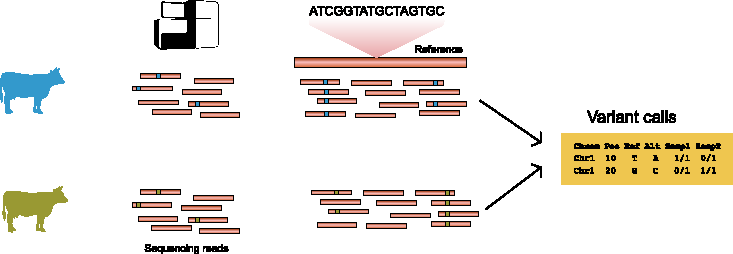
\includegraphics[width=\textwidth]{intro/fig1.pdf}
        \vspace{3mm}
        \caption[Identification of genetic variants through re-sequencing]{\textbf{Identification of genetic variants through re-sequencing} \\
        \footnotesize{Whole-genome sequences were fragmented into billions of short fragments which were then read by DNA sequencer in a massively parallel manner. The sequencing reads were compared (aligned) to the reference genome. Genetic variants were identified as nucleotide discordances relative to the reference sequences.}}
        \label{fig11:reseq}
\end{figure}


\section{Improvements in the cattle reference genome} 

A well-annotated reference genome is the starting point for many genomic analyses. It serves as a reference point for read alignments, variant calling, gene annotation, and functional analysis. Gene loci are defined at specific genomic coordinates, and alleles are referred to as alternative or reference  nucleotides. The ability to compare billions of sequencing reads from hundreds to thousands of individuals to the reference sequences has quickly become the gold standard, identifying variants underpinning  inherited diseases or other relevant traits, thus accelerating genetic progress \citep{bickhart2020symposium}.

The first cattle reference genome (Btau 3.1 and Btau 4.0) was assembled in 2009 from bacterial artificial chromosome (BAC) and whole-genome shotgun (WGS) sequencing \citep{elsik2009genome}. The contig and scaffold N50 for this assembly were 48.7 kb and 1.9 Mb respectively. This assembly was further refined in 2014 to close gaps and correct structural errors (UMD\_3.1.1) using additional sequencing data and sophisticated assembly approaches \citep{zimin2009whole}. The most recent cattle reference genome (ARS-UCD 1.2) was assembled using single-molecule real-time (SMRT) long-read sequencing data and scaffolded with optical mapping data. The quality of the resulting assembly improved considerably over UMD3.1 with contig and scaffold N50 values of 25.89 Mb and 103 Mb, respectively \citep{rosen2020novo}. Advances in assembly techniques (e.g., trio binning) and the development of highly accurate long-read sequencing technology now enable the construction of assemblies of high continuity, correctness and completeness \citep{bickhart2020symposium}. The recently generated assemblies exceed in quality the current bovine reference genome with contig N50 of larger than 70 Mb and could resolve complex genomic regions, e.g. major histocompatibility regions \citep{rice2020continuous}. Trio binning takes advantage of the high heterozygosity in hybrids to separate long reads according to parental origins. The assembly is subsequently performed separately from the partitioned reads resulting in two haplotype-resolved assemblies. This approach  was first applied  to a cross between \emph{Bos taurus} x \emph{Bos indicus cattle} (Angus x Brahman) \citep{koren2018novo}, but now has been applied to broad range cattle breeds, including  undomesticated and/or cattle relatives (Yak, Gaur, Bison) \citep{oppenheimer2021reference}. Recently, the Bovine Pangenome Consortium \citep{heaton2021reference} was initiated to coordinate genome assembly efforts and characterize the complete diversity from hundreds of global cattle breeds, including the wild-relatives and under-represented breeds. 

\section{One reference genome is not enough}

\subsection{A single linear genome cannot fully represent species diversity}

Despite recent spectacular quality improvements, the linear reference genomes still poorly represent the full genomic diversity within a species. A linear reference genome typically represents a mosaic haplotype of either one or a few individuals. For example, the current cattle reference genome (ARS-UCD1.2) was assembled from a DNA sample from a single highly-inbred animal from the Hereford breed named Dominette, which was initially selected to simplify the assembly process \citep{rosen2020novo}. Reference assemblies from  other livestock species were generated using a similar approch, e.g., Duroc breed used for Sscrofa11.1 pig reference \citep{warr2020improved}, San Clemente breed for domestic goat reference \citep{bickhart2017single}, and boxer breed for  CanFam 3.1 dog reference \citep{lindblad2005genome}. While the selection of reference animals seems to be trivial, the resulting reference sequences do not necessarily reflect the most common allele in the population or from samples with the most ideal phenotypes \citep{ballouz2019time}. Reference-guided variant discovery might reflect some properties of the reference animal rather than the population; e.g., variant calling will output more variants when the reference  contains rare alleles. \citet{Low2020} found a striking difference in the number of polymorphic sites when calling Angus variants from an Angus reference than from a Brahman reference. Additionally, the reference genome might carry the lower frequency variants or variants private to the reference animals. \citet{shukla2019hg19kindel,ballouz2019time} estimated that 2 million bases in the human reference genome are minor alleles. 

\subsection{Insufficient representation of genetic diversity by linear genomes cause reference bias}

Because alignment algorithms compare the reads towards the reference and try to minimize differences, the reference-guided variant discovery is biased towards the reference bases. In other words, it is easier to align DNA fragments without differences to the reference bases than DNA fragments  that contain non-reference bases. Comparison of the sequencing reads with variants, even if they are the true representation of that species, will be penalized, resulting in sub-optimal alignments, misalignments, or cannot be mapped (Fig. \ref{fig12:bias}) \citep{pritt2018forge}. Together, this limitation is referred to as \textbf{soft reference bias}, which hampers genomic analysis that depends on the allelic balance such as heterozygous variant calling \citep{garrison2018variation}, allelic-specific expression \citep{salavati2019elimination}, or analysis in the highly polymorphic regions \citep{dilthey2015improved}. \citet{wu2018pervasive} observed the impact of reference bias affecting a lower estimate of divergence among\emph{ Bos} species due to mapping of cattle-relatives data to the \emph{Bos taurus} reference genome, which tends to overlook the diverged regions. 

Another limitation is referred to as \textbf{hard reference bias}, whereby a single reference is a poor representation of large structural variations that diverged between individuals in the population (Fig. \ref{fig12:bias}) \citep{colquhoun2020nucleotide}. Reads originating from these highly diverged segments will remain unmapped and all subsequent genomic analyses will be blind to variations in these “missing” regions. In cattle, the comparison between two taurine assemblies revealed 10.9 Mb of Angus-specific sequences that were not present in the Hereford-based reference assembly \citep{Low2020}. This number increases to 21.8 Mb when the Angus assembly is compared to an indicine cattle genome. Reference genomes lacking millions of bases has been observed in many species. \citet{ameur2018novo,audano2019characterizing} estimated that each human genome on average carries about 10 Mb non-reference bases. Long read data analysis across global ancestries discovered 8.5 Mb insertions observed in majority of the human population \citep{audano2019characterizing}. Remarkably, an analysis of the unmapped reads of the African pangenome revealed 300 Mb non-reference insertions, suggesting that the existing human reference genome might lack diversity spanning 10\% of the genome (Sherman et al. 2019). \\

\bigskip

\begin{figure}[!htb]
    \centering
    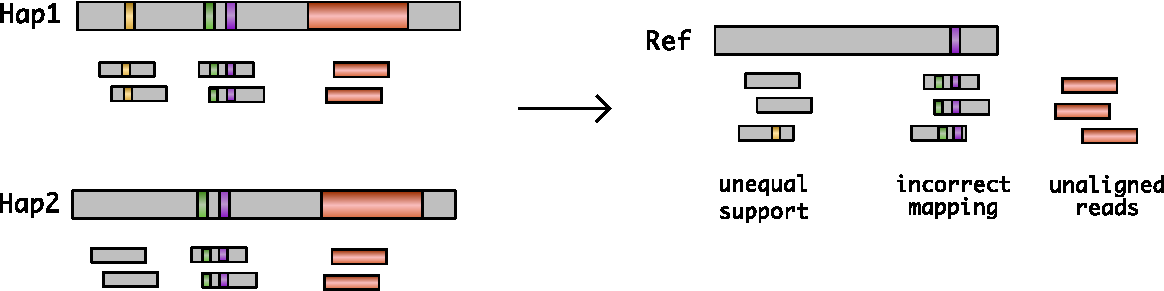
\includegraphics[width=\textwidth]{intro/fig2.pdf}
        \vspace{3mm}
        \caption[Illustration of the reference allele bias]{\textbf{Illustration of the reference allele bias.} \\
        \footnotesize{The origin of short sequencing reads of the sample (hap1 and hap2) are determined by alignments to the reference nucleotides. Thus, the comparison will always be biased towards nucleotides in the reference. Alignment of reads with alleles differing from reference might receive lower support than allele matches to the reference nucleotides (yellow stripe), results in incorrect alignments with multiple variations (green and purple stripes), or remain unmapped if the regions not present in the reference (e.g., large insertion, orange box). Grey background denotes reference sequences.}}
        \label{fig12:bias}
\end{figure}

\subsection{The problem of reference bias is pronounced in a species with high genetic diversity}

The effect of reference bias will be more pronounced in a highly diverged species like in cattle. Genetic architecture of the bovine genomes has been shaped by various processes related domestication, admixture, introgression, local adaptation, and human-directed selection \citep{zhang2020evolution}, resulting in the creation of more than 600 subpopulation (known as breeds) adapted for a variety of environmental conditions and selected for various breeding goals. Genetic diversity is higher in cattle than human populations \citep{charlier2016ngs}. The bovine species formed the bovine tribe which subdivided into three sub-tribes diverged about 10-15 million years ago: the \emph{Pseudorygina},\emph{ Bubalina} (Buffalo), and \emph{Bovina} (genus Bison and Bos). Specifically, the subtribe bovina is comprised of three subtribes split about 3-5 million years ago: (i) yak, bison; (ii) gaur,gayal, and banteng; and (iii) taurine and zebu \citep{pitt2019domestication}. Generally, Taurine breeds (\emph{Bos taurus taurus}) are intensively selected for production traits (milk and beef) and have higher fertility than indicine breeds. Indicine breeds (\emph{Bos taurus indicus})  generally have lower production traits and fertility, but still possess desirable traits related to heat tolerance, parasite and disease resistance \citep{Low2020}. However, these characteristics are not strict as there are numerous local cattle breeds optimized for specialized breeding goals \citep{signer2017population,upadhyay2019genomic}. Series of introgressions and hybridizations created specialized breeds with mosaic genomes, such as Brahman, composed of ~10 \% taurine and 90\% indicine origin \citep{koufariotis2018sequencing}. African cattle are generally admixture between \emph{Bos taurus} x \emph{Bos indicus}, where the introgressed regions are selected for African pastoralism \citep{kim2020mosaic}. On average, each individual cattle carry more than 5 million variants relative to Bos taurus reference, which is higher than variations reported in the human population at about 3-4 million variants \citep{daetwyler2014whole,sudmant2015integrated}. The number of variants is higher in more diverged, indicine \citep{koufariotis2018sequencing} or under-studied African cattle \citep{kim2020mosaic,kim2017genome}. Additionally, this amount likely underestimates the actual genetic diversity as it does not consider the structural variations, which are poorly characterized with short-read sequencing technology \citep{mahmoud2019structural,chaisson2019multi}. 

\section{Strategies to mitigate reference bias}

\subsection{Modification of the existing linear reference genome}

Some strategies have been proposed to mitigate the reference bias. The most straightforward solution is to create a so-called consensus reference genome, whereby each minor allele in the reference sequence is replaced by the most frequent allele in the population. Since the transformed reference is still in the linear space, the downstream genetic analysis can still use the tools currently developed for linear genomes. However, a coordinate lift-over is needed when indels are included in the substitutions. \citet{ballouz2019time} built consensus human reference by replacing 2 million minor alleles with the corresponding major allele, that reduced mapping error by a factor of three and improved the quantification of transcripts \citep{kaminow2020virtue}. \citet{chen2021reference} extended this idea into a so called reference flow approach, whereby it re-aligned sub-optimally mapped reads into a set of genomes from multiple population, that could reduce strongly heterozygous sites by 22\%. Another effort, as in the human genome, is by continually expanding reference with alternative contigs in the polymorphic regions that are impossibly represented with a single haplotype. There were currently 13 updates with 261 alternate patches that add 109 Mb total length. However, this strategy is not sustainable with more diversity included. Additionally, the lack of tools that can properly handle these additional overlapping contigs will likely not be able to mitigate the reference bias \citep{sherman2020pan}. 

\subsection{Creation of population-specific genome assemblies}

The reduced cost of long-read sequencing and improved assembly techniques  make it easier to generate high-quality, near error-free, and complete genome assemblies \citep{miga2020telomere,logsdon2021structure}. Thus, more studies have now shifted from species-level references into population-specific reference genomes, effectively creating more personalized genomes. Large genomic initiatives such as Vertebrate Genome Project (VGP, \url{https://vertebrategenomesproject.org/}), Darwin Tree of Life (\url{https://www.darwintreeoflife.org/}), or Earth Bio-genome Project \citep{lewin2018earth} contributes to the explosion the number of genome assemblies across the tree of life accessible in the public domain. The first phase of VGP generated 268 vertebrate genomes using long-read data, that were further scaffolded with optical mapping to produce chromosome-scale assemblies fulfilling the strict high-quality criterias \citep{Rhie2021}. On the other hand, some genomic initiatives focus to deeply characterize the diversity of a single species, such as the Human Pangenome Reference Consortium (HPRC) that plans to generate 350 human assemblies representing global ancestries (see \url{https://humanpangenome.org/}). A similar internationally coordinated effort was also initiated for cattle with the Bovine Pangenome Consortium \citep{heaton2021reference} that aim to generate reference-quality assemblies across global cattle breeds. There are already dozens of genomes from livestock species publicly available in the public repository. As of April 2021, there are chromosome-level assemblies of 22 cattle (\emph{Bos}) and its relatives (gaur, gayal, yak, bison), 19 pigs (\emph{Sus}), 7 sheeps (\emph{Ovis}), 4 goats (\emph{Capra}), 9 dogs (\emph{Canis}), with many more continuing to be added.

\section{Transition from genomics to pangenomics}

\subsection{Definition of the pangenome}

A pangenome refers to a structure used to  integrate multiple genomes, reflecting the complete species diversity rather than collapsing all variations into a single haplotype, see recent reviews \citep{bayer2020plant,sherman2020pan,della2021pan}. The term pan-genome (pan – whole, Greek) was first introduced by \citet{tettelin2005genome} to describe complete gene repertoire across \emph{Streptococcus agalactiae} strains where 20\% of the genes are variable across isolates. This concept was quickly adopted across the tree of life, including the agriculturally important plant and animal species, such as pig \citep{li2017comprehensive,tian2019building}, goat \citep{li2019towards}, and human \citep{duan2019hupan,sherman2019assembly}. There has been rapid growth in the number of pangenome publications across years \citep{bayer2020plant}, with close to 8000 studies indexed by PubMed,  although most currently focus on bacterial pangenomes.  

\subsection{Categorization of the pangenome}

The content of a pangenome may be divided into the core and flexible genome (also known  as dispensable or accessory genome, Fig. \ref{fig13:pan}a). Core genome is common sequences across all individuals that is responsible for maintaining essential function (e.g., DNA replication, cellular homeostasis and cellular processes). This part of genomes is under purifying selection, thus having less diversity. Dispensable genomes are segments that vary across individuals. They are under less evolutionary constraint, which allows for contributions to numerous adaptive phenotypes, mainly disease, biotic, and abiotic resistance, survival, immunity, defence response, adaptation to new environments, communications, and signalling \citep{golicz2020pangenomics}. Thus, dispensable genomes are of particular interest for the studies of adaptive traits that might drive genetic differentiation and give population their distinguishing characteristics. In animals, the pangenome is largely dominated by core component (e.g., 96.67\% of genes in the human) \citep{duan2019hupan}. However, a recent report in the Mediterranean mussel \emph{Mytilus galloprovincialis}, with high-stress tolerance and lineage-specific duplications, indicates that up to 25\% of the total genome is variable \citep{gerdol2020massive}. Pangenomes have been extensively characterized in plants, among them are in rice \citep{zhao2018pan}, tomato \citep{gao2019tomato}, wheat \citep{walkowiak2020multiple}. They reported larger proportion of accessory genomes (>20\%), particularly in polypoid, outcrossing, or species history of whole-genome duplications \citep{tao2019exploring}. Higher ratio of flexible to core genome indicates a species with higher adaptability \citep{tranchant2018plant}. 

It is important to consider whether the pangenome is of either closed or open type. In a closed type pangenome, the sequencing of sufficient samples will capture the whole pangenome, and thus the size of the complete pangenome can be computationally predicted. On the other hand, sequencing more individuals will recover more pangenome content in an open pangenome. Thus, the size of pangenome keeps increasing as more samples included \citep{golicz2020pangenomics}. Many plant and animal pangenomes are a closed type in terms in the number of genes but open in terms of total sequence content \citep{duan2019hupan,golicz2020pangenomics}, which also suggests that the non-coding segments primarily drive the sequence variability across individuals. Bacterial pangenomes  are generally open type due to prevalence of horizontal gene transfer \citep{soucy2015horizontal}. Sampling bias of underrepresented diversity (such as genetically related samples) could lead to the falsely concludingthe pangenome is complete \citep{tranchant2018plant}. With additional, sufficiently  diverged samples, the  pangenome would continue to grow. Thus, sampling strategy in a pangenome study should maximize diversity to fully retrieve the complete pangenome. 

\begin{figure}[!htb]
    \centering
    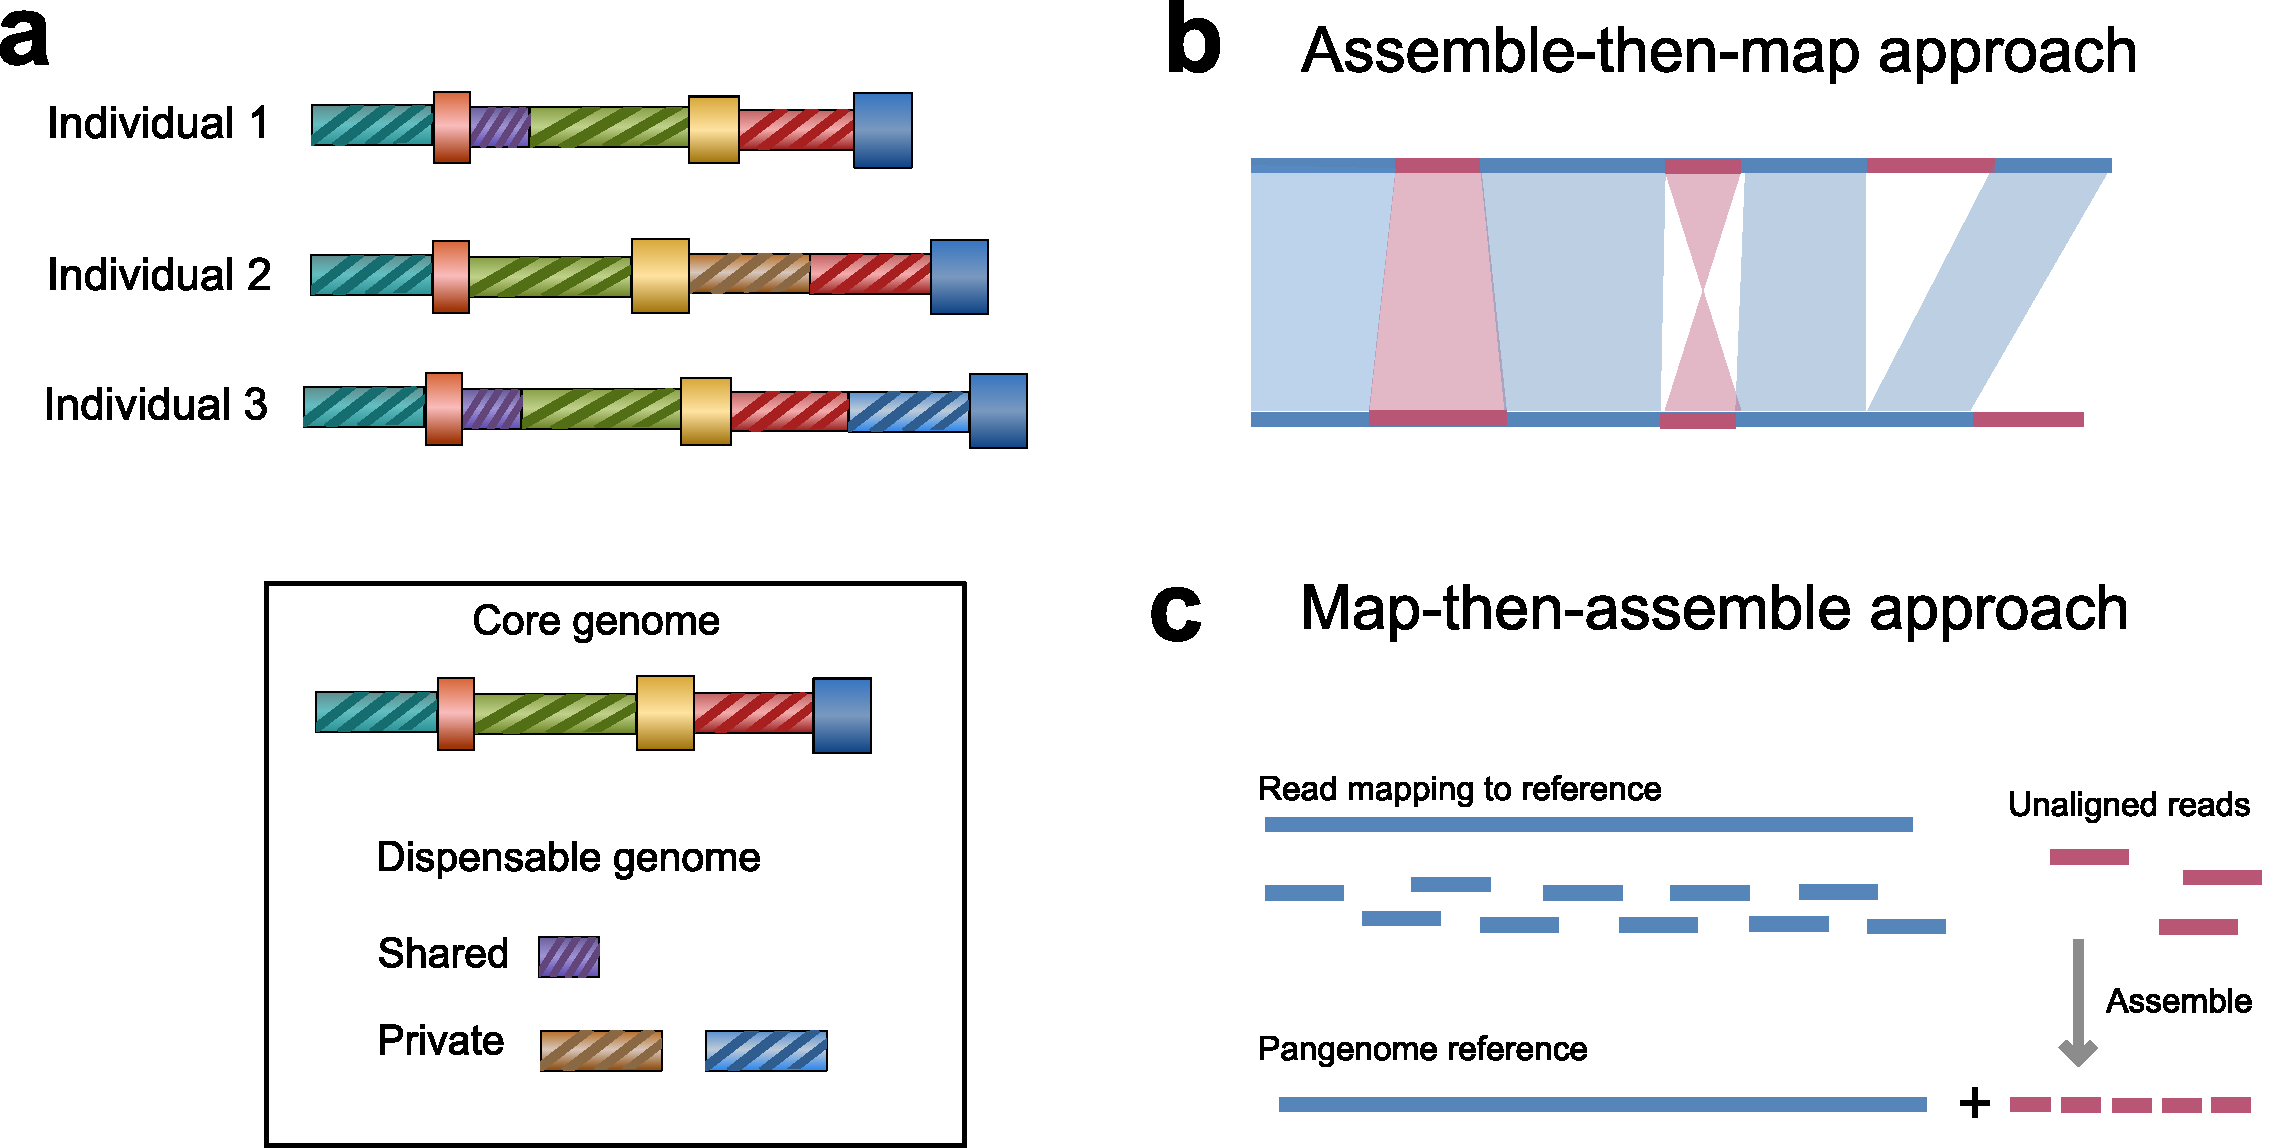
\includegraphics[width=\textwidth]{intro/fig3.pdf}
        \vspace{3mm}
        \caption[The concept of pangenomes]{\textbf{The concept of pangenomes.} \\
        \footnotesize{\textbf{(a)} Pangenomes refers to a collection of individual genomes in the populations, which is further divided into core (shared by all members of populations) and flexible parts that the presence varies across individuals. Different strategies to build the pangenome \textbf{(b)} Assemble-then-map: Genomes from multiple individuals are assembled, which are then compared to the reference assembly \textbf{(c)} Map-then-assemble: sequencing reads from multiple individuals are aligned into the reference. Unmapped sequences assembled and added as additional contigs to the reference sequences. Figures are adapted from \citep{sherman2020pan} and \citep{bayer2020plant}.}}
        \label{fig13:pan}
\end{figure}


\subsection{Approaches to build a pangenome}

There are two commonly used approaches to build a pangenome (Fig. \ref{fig13:pan}bc): “assemble-then-map" and “map-then-assemble" (also known as map-to-pan) \citep{golicz2020pangenomics}. In the “assemble-then-map"-strategy, each genome is assembled and annotated independently, which is then followed by pairwise alignment of all assembled genomes to determine shared and non-shared segments \citep{duan2019hupan,li2019towards,eisfeldt2020discovery}. This assembly-based strategy is supposed to recover the full-length non-reference sequences and resolve repetitive and complex structural variants. However, this approach depends on the assembly contiguity and completeness. Assembly and annotation errors make the comparison difficult and may lead to erroneous identification of the structural variations. Additionally, genome assemblies are still too expensive to be performed on the population-scale, limiting analysis only on a subset of individuals. To take advantage the massive amount of population-scale of the short-read sequencing data, the majority of  recent pangenome studies utilize the “map-then-assemble"-approach \citep{holden2018assembly,laine2019exploring,sherman2019assembly}. Sequencing reads from each sample are independently mapped to the reference genome. The  unmapped (or poorly mapped) reads are subsequently assembled to obtain the non-reference sequences. However, due to the nature of short-read-based assembly, most of the resulting contigs are fragmented, making it difficult to locate the breakpoints’ origins in the reference genome \citep{sherman2019assembly}. 

\section{Graph-based pangenomics}

\subsection{Graphs as richer reference structures to integrate the genetic diversity}

The pangenome approaches based on unmapped reads or assembly comparison, as discussed above, rely on collections of linear genomes and do not attempt to provide coherent representation that relates all genomes. Considering the prevalence of genetic variations across individuals in the population and availability of abundant genomic resources, the linear representation is clearly an oversimplification. Emerging pangenome methods are developed to build richer variation-aware reference structures that unify the complete genetic diversity of a species in a non-redundant way. These collective efforts led to a new genomic discipline known as Computational Pangenomics, see review \citep{paten2017genome,computational2018computational,eizenga2020pangenome}.

Graph-based models (also known as genome graphs or sequence graphs) are currently proposed as data structures that unify a collection of related sequences in a compact way (Fig. \ref{fig14:graph}). In a sequence graph, nodes are commonly labelled with sequences and directed edges connect nodes with continuous sequences. Regions without differences are collapsed into a single node allowing compression of redundant sequences. Regions where the sample differs from each other form bubbles, with alternate paths representing different alleles \citep{paten2018superbubbles}. Traversing (or walk through the graphs) recovers the initial input sequences as well as all possible recombinations. 

\begin{figure}[!htb]
    \centering
    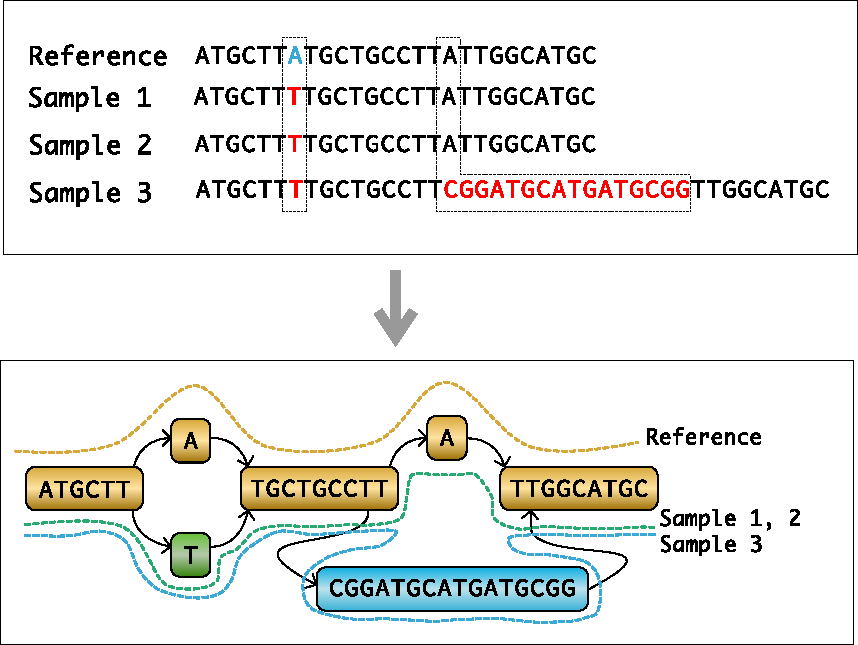
\includegraphics[width=0.8\textwidth]{intro/fig4.pdf}
        \vspace{3mm}
        \caption[Graph-based pangenome approach]{\textbf{Graph-based pangenome approach.} \\
        \footnotesize{\textbf{(a)} The majority of the pangenome studies follow the classical pangenome approach, where multiple linear genomes are compared without compressing redundant information and might lack orthology relationships. \textbf{(b)} Graph-based pangenome approach offers unified and richer multiple genomes representation. Nodes contain DNA sequences and nodes with continuous sequences connected with directed edges. Redundant information across genomes is compacted by collapsing invariant regions into a single node. Alternative nodes in the bubbles (green and blue nodes) are alleles in the population. Thus, graphs allow sequence comparison to occur in the context of variations. Walks through the graph might retrace the original sets of sequences from which it was built (dashed line).}}
        \label{fig14:graph}
\end{figure}



\subsection{Graph genomes implementations}

The first pangenome graph implementation was based on the DBG (\emph{De Bruijn Graphs}). Sequencing reads from all samples were fragmented into $k$-mer length $k$, and the graph was constructed by inducing the first and second node where $k-1$ bp end of first node that overlap with the $k-1$ bp start of the second node. Nodes are “coloured” where each colour map to the origin of the samples. \citet{iqbal2012novo} developed \emph{Cortex}, a coloured DBG-based pangenome tool. They used it to construct a population graph from 164 human samples and identified 3.2 Mb novel sequences that are absent in the human reference genome. Because the genomic coordinates are discarded by fragmenting the reads, DBG-based approaches are not suitable for resequencing study, although a recent study attempts to embed a long-range path information into the graph \citep{turner2018integrating}. 

Current well-established graph genome implementations establish a variation graph as an extension of the linear reference genome \citep{eggertsson2017graphtyper,garrison2018variation,sibbesen2018accurate,rakocevic2019fast,kim2019graph}. This implementation utilizes the existing linear reference genome as a backbone, which is then augmented with known variants. To build the graph, reference sequences are split at variable sites, and variants are added as alternative nodes of the reference bases in the graphs. The linear reference coordinates are embedded in the graphs as a path, and the nodes are referred to relative to this reference path. Thus, the reference path provides a stable coordinate system that can be used as a basis for alignment and annotation \citep{garrison2018variation}. 


\emph{Graphtyper }is the first open-source variation graph-based software designed for genotyping from a local (region-specific) graph \citep{eggertsson2017graphtyper,eggertsson2019graphtyper2}. It uses a variant file (\emph{VCF}) as input source of variant sites and a reference assembly as backbone of the graph. Because of the limited variations modelled by a VCF file, the output graph is directed and acylic containing insertions and deletions but not necessarily complex variations (Fig. \ref{fig15:mut}b). \emph{Graphtyper} applies a two-step genotyping proces. The  “discovery step” is similar to linear reference-guided variant analysis. Sequencing reads are mapped to the linear genome and variants are identified from the alignments. This step is then followed by read realignment towards local graphs. To this end, \emph{Graphtyper} first constructs small regional graphs of 10 kb windows that are subsequently augmented with variants discovered during the first step. Then, \emph{Graphtyper} extracts reads that were initially mapped by the linear mapper, realigns them onto the local graph and performs the variant genotyping from the refined alignments. This approach, however, does not  fully  eliminate reference bias because it relies on the global read placement by a linear mapper. However, this design makes it highly efficient as evidenced with scalable joint genotyping of close to 50,000 Icelander samples \citep{eggertsson2019graphtyper2}. Additionally, Graphtyper outperformed current state-of-the-art linear genome-based tools (e.g., \emph{SAMtools} and \emph{GATK}), particularly from more refined variants surrounding Indels with considerably reduced Mendelian errors \citep{eggertsson2017graphtyper}.

\begin{figure}[!htb]
    \centering
    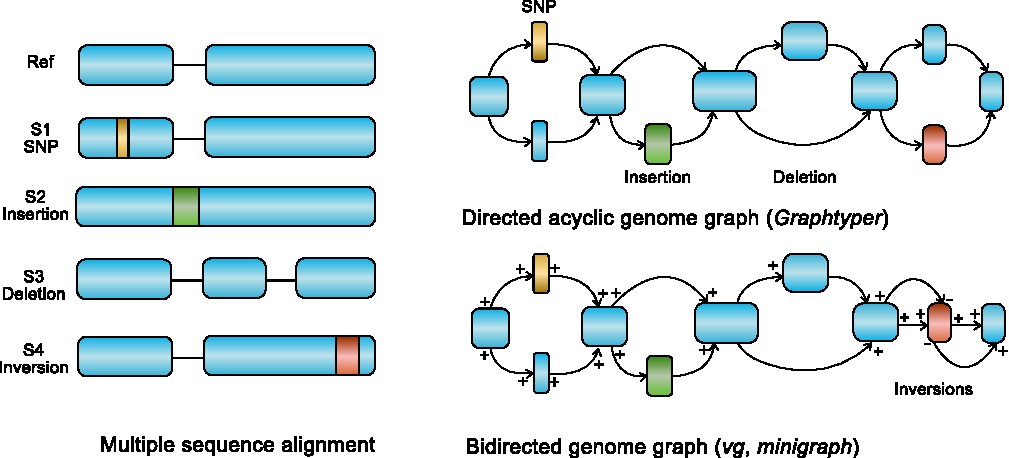
\includegraphics[width=0.9\textwidth]{intro/fig5.pdf}
        \vspace{3mm}
        \caption[Genetic variant representation in the genome graphs]{\textbf{Various genome graph implementations and representations of variations in the graphs} \\
        \footnotesize{\textbf{(a)} multiple sequence alignments capturing sequence relationships. \textbf{(b)} directed genome graphs underlying the data structure of \emph{Graphtyper}; a similar to multiple sequence alignments but with compressing redundant information. \textbf{(c)} general bidirected sequence graph as implemented in \emph{vg} that each edge endpoint has independent orientation. Note  forward (+) and reverse strand (-) to indicate inversions (orange). Figures are adapted from \citep{eizenga2020pangenome}.}}
        \label{fig15:mut}
\end{figure}

\subsection{Construction of the whole-genome variation graphs with the \emph{vg toolkit}}

The variation-graph toolkit (\emph{vg}) is the first open-source toolkit designed to perform the full suite of genome analyses from genome graphs in species with a gigabase-sized genome \citep{garrison2018variation}. The basic structure of \emph{vg} is a bidirected sequence graph that can express the strand-ness of the input sequences (Fig. \ref{fig15:mut}c). Each edge endpoint has an independent orientation to indicate whether the forward or reverse sequences are spelled out when visiting the node \citep{paten2017genome}. Therefore, \emph{vg} can represent variations with complex topology e.g., inversion or translocation. Haplotype information from the sample are stored in an auxilary index so that analysis from the graph can consider haplotype information \citep{siren2020haplotype}. Graph mapping in \emph{ vg} is optimized for short–sequencing reads that follows the seed-and-extend paradigm. It relies on a \emph{GCSA2 }graph index (a generalization of linear genome-based\emph{ BWT} index to graphs) for a fast seed query \citep{siren2017indexing}. The index construction is the computationally most demanding step because all $k$-bp paths in the graphs need to be enumerated, which is intractable in complex regions with high variant density. In practice, \emph{vg} can handle complex region by indexing on a simplified graph e.g., retaining only biologically plausible paths informed by the haplotype index \citep{siren2017indexing}. Graph mapping is computationally more expensive than linear mapping because multiple alternative paths need to be explored. To make graph-based mapping competitive to linear mapping, \emph{vg mapper} is currently being improved to utilize minimizer-based mapping paradigm and restrict the mapping that conforms the haplotype paths. It can achieve the same mapping speed as the \emph{BWA} linear mapper with more accurate alignment performance, especially for application related to structural variant genotyping \citep{siren2020genotyping}. 

\section[Construction of the multi-assembly graphs]{Genome graph construction from a collection of reference-quality assemblies}

\subsection{Multi-assembly graphs as a platform to integrate multiple genome assemblies}

The construction of graphs by augmenting a reference genome with a predefined set of variants  is still somewhat biased to the reference allele, because the variations are discovered with respect to the reference genome. Additionally, variant identification based on the read alignment is limited by the read length, and thus cannot reliably identify large structural changes between individual genomes \citep{feng2020higher}. Moreover, the input variant file format (VCF) can only model simple variations and is not suitable for representing complex structural variations (e.g., SNPs nested inside long insertions) \citep{letcher2021enabling}.  Building a graph directly from a collection of genome assemblies is a better approach to capture more comprehensive genetic variation. Such a graph will encompass more types of genetic variations, including large structural changes that differ between assemblies (so-called non-reference sequences) that are currently not accessible from linear genomes. This effort will be highly relevant to exploit an ever-increasing number of reference-quality genome assemblies that are being produced at unprecedented rate in order to perform integrative and comprehensive comparative genomics across these resources. 

In the multi-assembly graph approach, graphs are constructed from the multiple whole-genome alignments. Segments which are present in multiple assemblies without sufficient variation are collapsed into a common node,representing conserved regions or core genomes shared in multiple input samples. The variable regions form bubbles containing multiple paths of the segments that differ (of poorly or non-aligned sequences) between assemblies. Thus, bubbles in the graph represent structural variations across assemblies, with different paths being different alleles. 

\subsection{Strategies to build multi-assembly graphs}

Accurate multi-genome alignment is the key for the multi-assembly-based graph approach. However, multiple genome alignment is computationally demanding and scales poorly with the number of genomes. Recently an efficient multiple-genome alignment approach has been implemented in the \emph{Cactus Progressive} software \citep{armstrong2020progressive} that scales to hundreds or even  thousands of genomes while maintaining high alignment accuracy. The key to its computational efficiency and accuracy is dividing a large whole-genome alignment problem into smaller sub-alignment problems using a guide tree. Whole-genome alignment of more than 600 mammals and birds species using Cactus facilitate a thorough comparative genomics across vertebrate phylogeny \citep{feng2020dense,Genereux2020}.
\citet{hickey2020genotyping} applied the \emph{vg toolkit} to induce graphs from \emph{Cactus} alignment of 12 yeast strains. They could map more reads with higher mapping quality, mostly due to mapping improvement in the regions harbouring complex structural variations missed from read alignment-based method. 

The approximate mapping between assemblies is another approach to construct multi-assembly graphs. \emph{Minigraph} \citep{li2020design} has recently been developed as a multi-genome graph constructor that extends the minimizer-mapping capability of minimap2 into a graph \citep{li2018minimap2}. It can establish a pangenome graph from 20 human assemblies in under 3 hours with less than 100 GB of memory. The tool applies an incremental graph generation. It uses  a selected genome as a backbone of the graph which is then iteratively augmented with unaligned or poorly mapped segments from the other assemblies. \emph{Minigraph} simplifies the general bidirected sequence graph data model resulting in a faster and a more straightforward graph analysis. For example, it enforces linearity of the input genomes that produces graph containing insertions and deletions between genomes but ignoring events that breaks the linearity, such as translocations. Constraining alignment to an anchor genome also ensures that the graphs devoid of complex and highly tangled parts which are difficult to interpet \citep{Lei2021}. Comparative genomics using a pangenome graph built with \emph{minigraph} containing human and its closely related ape species revealed important biological insights, including the evolution of repeat-rich regions in primates \citep{li2020design}, inaccessible  with a linear genome. An unpublished graph pipeline (Pangenome Graph Builder, \url{https://github.com/pangenome/pggb}) aims to build a comprehensive reference-free graph containing all classes of genetic variations with paths that can reconstruct the entire input sequences. However, this method is still in the infancy and requires further testing. \\

\begin{figure}[!htb]
    \centering
    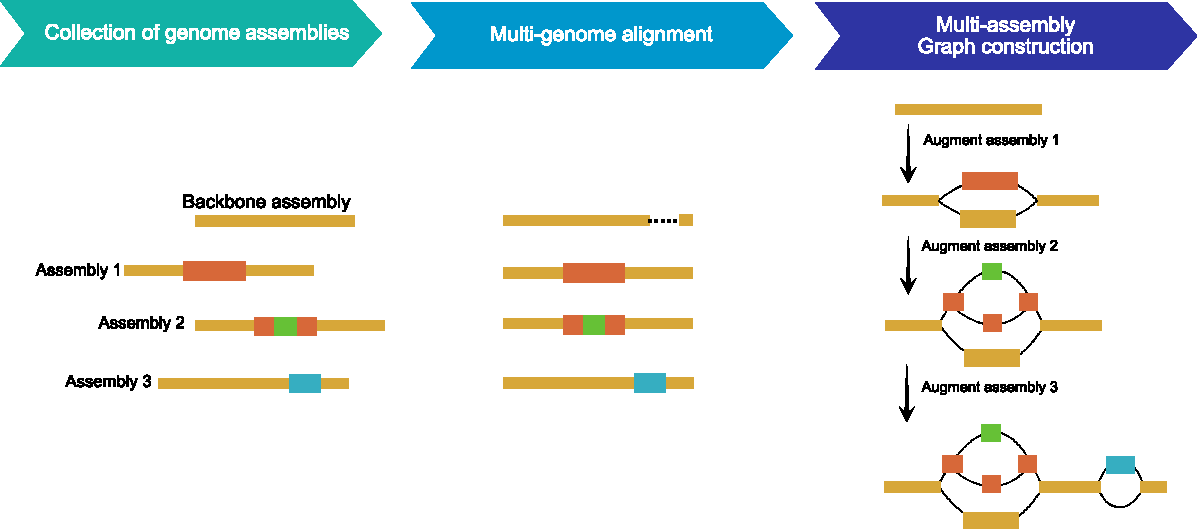
\includegraphics[width=\textwidth]{intro/fig6.pdf}
        \vspace{3mm}
        \caption[Construction of the multi-assembly graphs]{\textbf{Construction of the multi-assembly graphs} \\
        \footnotesize{Multi-assembly graph is built based on multi-genome alignment from the collections of genome assemblies (\emph{left}, \emph{middle}). In the \emph{minigraph} approach (\emph{right}), the graph is built iteratively from alignment of the genome to the backbone or to the existing graphs, which is then augmented with diverged sequences from the alignment.}}
        \label{fig16:multi}
\end{figure}

\section[Utilization of the graph genomes]{Utilization of graph genomes for genomic analyses}

Graph genome approaches have been applied in a wide range of genomic analyses, but largely have only been applied to human or plant genomes. These analyses were initially restricted to challenging regions such as the highly polymorphic Human Leukocyte Antigen (HLA) region \citep{dilthey2015improved,lee2018kourami}, where graph-based methods outperform gold-standard linear-genome genotyping. Multiple studies \citep{eggertsson2017graphtyper,garrison2018variation,sibbesen2018accurate,rakocevic2019fast}
 then assessed the performance of graph-based methods on whole-genome variant discovery and genotyping. \citet{garrison2018variation} constructed a global human graph that contained 80 million variants catalogued by the 1000 Human Genome Project. They showed that genome graphs enable a considerable improvement in read mapping, particularly for the subset of reads that differs from the reference and substantial reduction in the bias of calling large indels. 

\citet{pritt2018forge} estimated that with carefully selected variants, genome graphs could rescue 1.2 million incorrectly mapped reads from 30-fold coverage of human whole-genome sequencing data compared to the linear reference. \citet{martiniano2019removing} applied the \emph{vg} graph framework to an ancient DNA sample to mitigate reference bias due to short and degraded DNA. The benefit of mapping to a graph translates to substantial improvement in calling indels with sufficient accuracy for population genomic inference. \citet{grytten2019graph} extended vg graph capability to analyse ChIP-Seq data. Using a pangenome  of \emph{A. thaliana}, they discovered transcription factor binding sites that are absent in the linear genome. Studying transcription-factor binding motif from \emph{vg} graphs, \citet{tognon2021grafimo} identified variations in regulatory regions affecting the gene expression that otherwise missed with a linear genome. 

Graph genome approaches were also rigorously exploited to investigate large (structural) variations. SV genotyping mainly relies on the indirect inference of abnormal read alignment profiles (such as depth or split mapping) because the alleles are not present in the reference assembly \citep{mahmoud2019structural}. Known structural variants can be reliably  genotyped once included in the graph, even with short-read data, because the sequencing reads can be directly aligned to the corresponding variants. \citet{siren2020haplotype} constructed a \emph{vg} graph from 167 thousand structural variations detected from long-read data across diverse human ancestry. Re-genotyping of 5202 short-read sequencing data using this graph considerably improves the SV genotyping. Further analyses lead to identification of thousands of expression quantitative trait loci (eQTLs) driven by these large variations, largely undetectable from the linear reference genome. \citet{liu2020pan}  applied a similar strategy in the recent soybean pangenome. Re-genotyping of 2898 sequenced samples from diverse accessions using a pangenome graph integrated from 26 line assemblies enabled identification of a hitherto unknown 10 kb insertion that is associated with a seed phenotype. 

\section{Applications of the pangenome}

\subsection{Pangenome analysis in plant genomes}

Pangenome studies in plants successfully identified a large number of genes not included in the reference and highlight the substantial contribution of large variations into the dynamic of the pangenome. For example, pangenome analysis on 3000 rice accession identified more than 10,000 genes not included in the reference \citep{wang2018genomic}. A considerable number of non-reference insertions associated with agronomic traits, including seed weight and flowering time were found from \emph{Brassica} pangenome constructed from eight long-read-based assemblies \citep{song2020eight}. Interestingly, GWAS signals from these insertions are significantly stronger than the standard SNPs-based association. Construction pangenomes from 725 tomato accessions, \citet{gao2019tomato} revealed 4873 genes absent from the reference genome and discovered 2 kb promoter insertions regulating fruit flavour that lost during domestication but present in the ancestral accession. An increasing number of studies shift towards the graph-based approach, which is pioneered by construction of a graph-based soybean pangenome \citep{liu2020pan}. 

\subsection{Pangenome analysis in human genomes}

In human genomics, pangenome analyses following the large scale re-sequencing initiatives reveal several important insights. The 1000 Genomes project  revealed that each genome carries more than two-fold regions affected by structural variations (8.9 Mb) than small variations (3.6 Mb) \citep{10002015global}. Importantly, they discovered 240 genes related to immunoglobulin and glycoprotein with homozygous (knock out) deletions in multiple populations, suggesting its dispensable role \citep{sudmant2015integrated}. Pangenome analyses focusing on the Icelandic population, \citep{kehr2017diversity} found a common 766 bp insertions (allele frequency of 0.65) associated with decreased risk of myocardial infarctions, where the signals are stronger than the SNPs-based association. A follow-up study based on 3622 samples sequences using Nanopore (the largest long-read-based pangenome study to date) found that Icelanders carries on average large insertions covering 10.02 Mb genomic regions and identified a tandem repeat motif strongly associated with height \citep{beyter2020long}. Application of the customized pangenome pipeline in Chinese Han population detected 29.5 Mb non-reference sequence, including 185 genes missing from the reference genome \citep{duan2019hupan}. \citet{sherman2020pan} reported markedly larger non-reference sequences from African pangenome suggesting the substantial underrepresentation of the African diversity in the reference.

\subsection{Pangenome analysis in livestock genomes}

Pangenome approaches have also been applied in the livestock species, although at a lower rate than the plants or humans. The most notable is the analysis of the 44 genomes spanning all extant Ruminant families reveal the genomic basis underlying the evolutionary innovations such as multi-chambered stomach, headgear, cursorial locomotion, and dentition \citep{chen2019large}. Initial livestock pangenome analyses in animals rely on the assembly of unmapped reads. For example, \citet{holden2018assembly} identified 4.6 Mb novel insertions from assemblies of non-aligned reads from three dog breeds including  novel insertions in six known disease-associated loci. Analysis of unmapped reads from the reference individual in song bird (\emph{Parus major}), \citet{laine2019exploring} uncovered 1822 genes missing in the reference annotation, including \emph{TRY1}, which is highly expressed in the reference bird. A similar effort to characterize the unmapped reads in the cattle reference animal discovered a number of parasite genomes which are likely to be associated with the reference animal as a host \citep{whitacre2015s}. 

With a rapid influx of high-quality assemblies, pangenome analysis in animals now transition into a more direct assembly comparison. Comparison between Angus (\emph{Bos taurus}) and Brahman (\emph{Bos indicus)} haplotypes-resolved assemblies \citep{Low2020} uncovered an extra copy of \emph{FADS2P1} gene, which is proposed to confer the heat resistance in \emph{Bos indicus}. Analysis of the unaligned sequences between 10 goat assemblies \citep{li2019towards} recovered 38.3 Mb non-reference insertions and identified 2 Mb assembly error in ARS-1 goat reference genome that includes prolactin gene region. Analysis of 12 Eurasian pig de-novo assemblies retrieved 72.5 Mb novel insertions absent in Duroc-based reference assemblies \citep{li2017comprehensive,tian2019building}. Additionally, they also discovered a non-reference insertion segregates at high frequency in Chinese breeds (but not in European breeds) encompassing the \emph{TIG3} gene region, which is important for fatty acid metabolism. 




\singlespacing
\footnotesize

% uncomment so that references appear on the same page
% \let\Origclearpage\clearpage
% \let\clearpage\relax


% \bibliographystyle{abbrvnat}
\bibliographystyle{unsrtnat}
\bibliography{references/introduction}
%\printbibliography[title=References]

% \let\clearpage\Origclearpage

\ifdefined\BuildingFromMainFile
\else
   \end{document}
\fi

\iftwoside
\cleardoublepage
\newpage
\fi

% paper 1 as chapter 2

\chapter[Feasibility of the bovine genome graphs]{\LARGE{Assessment of variant genotyping using local variation graphs}}
\label{chap:locgraph}
\subsection*{Preface: Bridging text between Chapter 1 and Chapter 2}
\onehalfspacing
\normalsize
This chapter assessed the feasibility of the genome graphs in cattle genome for variant genotyping; the first graph-based genotyping approach applied in any agricultural animal. The region-specific graphs were constructed using variations discovered from the sequencing cohort implemented using \emph{Graphtyper}. The genotyping pipeline was based on refined sequencing read alignment towards the local graphs. The genotyping analysis showed that graph-based approach using \textit{Graphtyper} is highly accurate, outperforming state-of-the-art methods based on linear reference e.g., \textit{SAMtools} and \emph{GATK}. \\

\bigskip

% I assessed \emph{Graphtyper} software for variant genotyping in cattle.
% \emph{Graphtyper} performed two round of genotyping. The first is to discover variants from linear
% genome. And the second round used the variants discovered in the first round to construct a local genome graph and used it to refine the genotypes. I discovered that \textit{graph genotyping} using \textit{Graphtyper} is highly accurate in cattle and outperform current approaches e.g., \textit{SAMtools, \emph{GATK}} that are based on linear reference. My work is the first to apply \textit{graph genome} for sequence variant genotyping in the livestock genome.  I implemented the graph genotyping pipeline and it is now publicly available at \\  
% \url{https://github.com/danangcrysnanto/Graph-genotyping-paper-pipelines}. \\ 

\begin{center}\fbox{\begin{minipage}{35em}

% \emph{Contribution}: Hubert Pausch and I conceived the study. Christine Wurmser generated the sequencing data. I wrote the graph genotyping pipelines and Hubert Pausch and I performed the analyses. Hubert Pausch and I wrote the manuscript. 

\emph{Contribution}: I participated in conceiving the study, analysing the results and writing the manuscript. I wrote the graph genotyping pipelines. 

\end{minipage}}\end{center}

% \onehalfspacing
\ifdefined\BuildingFromMainFile
\else
   \documentclass[../main.tex]{subfiles}
   \begin{document}
\fi


\graphicspath{{figure/}{../figure/}}

\onehalfspacing
\normalsize

\begin{abstract}   
\onehalfspacing
\small
\textbf{Background}: The genotyping of sequence variants typically involves as a first step the alignment of sequencing reads to a linear reference genome. 
Because a linear reference genome represents only a small fraction of sequence variation within a species, reference allele bias may occur at highly polymorphic or diverged regions of the genome. Graph-based methods facilitate to compare sequencing reads to a variation-aware genome graph that incorporates a collection of non-redundant DNA sequences that segregate within a species. We compared accuracy and sensitivity of graph-based sequence variant genotyping using the \emph{Graphtyper} software to two widely used methods, i.e., \emph{GATK} and \emph{SAMtools}, that rely on linear reference genomes using whole-genomes sequencing data of 49 Original Braunvieh cattle.   
\medskip

\textbf{Results}: We discovered 21,140,196, 20,262,913 and 20,668,459 polymorphic sites using \emph{GATK}, \emph{Graphtyper}, and \emph{SAMtools}, respectively. Comparisons between sequence variant and microarray-derived genotypes showed that \emph{Graphtyper} outperformed both \emph{GATK} and \emph{SAMtools} in terms of genotype concordance, non-reference sensitivity, and non-reference discrepancy. The sequence variant genotypes that were obtained using \emph{Graphtyper} had the lowest number of mendelian inconsistencies for both SNPs and indels in nine sire-son pairs with sequence data. Genotype phasing and imputation using the \emph{Beagle} software improved the quality of the sequence variant genotypes for all tools evaluated particularly for animals that have been sequenced at low coverage. Following imputation, the concordance between sequence- and microarray-derived genotypes was almost identical for the three methods evaluated, i.e., 99.32, 99.46, and 99.24 \% for \emph{GATK}, \emph{Graphtyper}, and \emph{SAMtools}, respectively. Variant filtration based on commonly used criteria improved the genotype concordance slightly but it also decreased sensitivity. \emph{Graphtyper} required considerably more computing resources than  \emph{SAMtools} but it required less than \emph{GATK}.   
\medskip  

\textbf{Conclusions}: Sequence variant genotyping using \emph{Graphtyper} is accurate, sensitive and computationally feasible in cattle. Graph-based methods enable sequence variant genotyping from variation-aware reference genomes that may incorporate cohort-specific sequence variants which is not possible with the current implementations of state-of-the-art methods that rely on linear reference genomes. 

\medskip
\textbf{Keywords}: Sequence variant genotyping, Genome graph, Variation-aware graph, cattle, Whole-genome sequencing

\end{abstract}

\newpage

\section{Introduction}

% \doublespacing 
\linespread{1.25}
\normalsize
The sequencing of important ancestors of many cattle breeds revealed millions of sequence variants that are polymorphic in dairy and beef populations \citep{Hoff2017,Stothard2015,Boussaha2016,Jansen2013}. In order to compile an exhaustive catalog of polymorphic sites that segregate in Bos taurus, the 1000 Bull Genomes consortium was established \citep{Daetwyler2014,Hayes2019}. 
The 1000 Bull Genomes Project imputation reference panel facilitates to infer sequence variant genotypes for large cohorts of genotyped animals thus enabling genomic investigations at nucleotide resolution \citep{Daetwyler2014,Pausch2017,Bouwman2018,Raymond2018}.

Sequence variant discovery and genotyping typically involves two steps that are carried out successively \citep{nielsen2011genotype,guo2014three,goodwin2016coming,pfeifer2017next}: first, raw sequencing data are generated, trimmed and filtered to remove adapter sequences and bases with low sequencing quality, respectively, and aligned towards a linear reference genome using, e.g., \emph{Bowtie} \citep{langmead2012fast} or the Burrows-Wheeler Alignment (\emph{BWA}) software \citep{li2009fast}. The aligned reads are subsequently compared to the nucleotide sequence of a reference genome in order to discover and genotype polymorphic sites using, e.g., \emph{SAMtools} \citep{li2009sequence} or the Genome Analysis Toolkit (\emph{GATK}) \citep{mckenna2010genome,van2013fastq,poplin2018scaling}. Variant discovery may be performed either in single- or multi-sample mode. The accuracy (i.e., ability to correctly genotype sequence variants) and sensitivity (i.e., ability to detect true sequence variants) of sequence variant discovery is higher using multi-sample than single-sample approaches particularly when the sequencing depth is low \citep{liu2013variant,cheng2014assessing,baes2014evaluation,kumar2014evaluation,depristo2011framework}. However, the genotyping of sequence variants from multiple samples simultaneously is a computationally intensive task, particularly when the sequenced cohort is large and diverse and had been sequenced at high coverage \citep{poplin2018scaling}. The multi-sample sequence variant genotyping approach that has been implemented in the \emph{SAMtools} software has to be restarted for the entire cohort once new samples are added.\emph{GATK} implements two different approaches to multi-sample variant discovery, i.e., the \emph{UnifiedGenotyper} and \emph{HaplotypeCaller} modules, with the latter relying on intermediate files in \emph{gVCF} format that include probabilistic data on variant and non-variant sites for each sequenced sample. Applying the \emph{HaplotypeCaller} module allows for separating variant discovery within samples from the estimation of genotype likelihoods across samples. Once new samples are added to an existing cohort, only the latter needs to be performed for the entire cohort, thus enabling computationally efficient parallelization of sequence variant genotyping in a large number of samples.  

Genome graph-based methods consider non-linear reference sequences for variant discovery \citep{rakocevic2019fast,eggertsson2017graphtyper,novak2017genome,garrison2018variation,sibbesen2018accurate}. A variation-aware genome graph may incorporate distinct (population-specific) reference sequences and known sequence variants. Recently, the \emph{Graphtyper} software has been developed in order to facilitate sequence variant discovery from a genome graph that has been constructed and iteratively augmented using variation of the sequenced cohort \citep{eggertsson2017graphtyper}. So far, sequence variant genotyping using variation-aware genome graphs has not been evaluated in cattle.

An unbiased evaluation of the accuracy and sensitivity of sequence variant genotyping is possible when high confidence sequence variants and genotypes are accessible that were detected using genotyping technologies and algorithms different from the ones to be evaluated \citep{li2018synthetic}. For species where such a resource is not available, the accuracy of sequence variant genotyping may be evaluated by comparing sequence variant to microarray-derived genotypes (e.g., \citep{Jansen2013,depristo2011framework}). Due to the ascertainment bias in SNP chip data, this comparison may overestimate the accuracy of sequence variant discovery particularly at variants that are either rare or located in less-accessible genomic regions \citep{li2014toward,malomane2018efficiency}.

In this study, we compare sequence variant discovery and genotyping from a variation-aware genome graph using \emph{Graphtyper} to two state-of-the-art methods (\emph{GATK}, \emph{SAMtools}) that rely on linear reference genomes in 49 Original Braunvieh cattle. We compare sequence variant to microarray-derived genotypes in order to assess accuracy and sensitivity of sequence variant genotyping for each of the three methods evaluated.

\section{Methods}
\label{chap2:met}

\paragraph{Selection of animals} 

We selected 49 Original Braunvieh (OB) bulls that were either frequently used in artificial insemination or explained a large fraction of the genetic diversity of the active breeding population. Semen straws of the bulls were purchased from an artificial insemination center and DNA was prepared following standard DNA extraction protocols.

\paragraph{Sequencing data pre-processing}

All samples were sequenced on either an Illumina HiSeq 2500 (30 animals) or an Illumina HiSeq 4000 (19 animals) sequencer using 150 bp paired-end sequencing libraries with insert sizes ranging from 400 to 450 bp. Quality control (removal of adapter sequences and bases with low quality) of the raw sequencing data was caried out using the \emph{fastp} software (version 0.19.4) with default parameters \citep{chen2018fastp}. The filtered reads were mapped to the UMD3.1 version of the bovine reference genome \citep{zimin2009whole} using \emph{BWA mem} (version 0.7.12) \citep{li2009fast} with option-M to mark shorter split hits as secondary alignments, default parameters were applied in all other steps. Optical and PCR duplicates were marked using \emph{Samblaster} (version 0.1.24) \citep{faust2014samblaster}. The output of \emph{Samblaster} was converted into \emph{BAM} format using \emph{SAMtools view} (version 1.3) \citep{li2009sequence}, and subsequently coordinate-sorted using \emph{Sambamba} (version 0.6.6) \citep{tarasov2015sambamba}. We used the \emph{GATK} (version 3.8) \emph{RealignerTargetCreator} and \emph{IndelRealigner} modules to realign reads around indels. The realigned BAM files served as input for \emph{GATK} base quality score recalibration using 102,092,638 unique positions from the Illumina BovineHD SNP chip and Bovine dbSNP version 150, as known variants. The \emph{mosdepth} software (version 0.2.2) \citep{pedersen2018mosdepth} was used to extract the number of reads that covered a genomic position.

\paragraph{Sequence variant discovery}

We followed the best practice guidelines recommended for variant discovery and genotyping using \emph{GATK} (version 4.0.6) with default parameters for all commands \citep{mckenna2010genome,vander2018best,depristo2011framework}. First, genotype likelihoods were calculated separately for each sequenced animal using \emph{GATK HaplotypeCaller} \citep{vander2018best}, which resulted in files in \emph{gVCF} (genomic Variant Call Format) format for each sample \citep{danecek2011variant}. The gVCF files from the 49 samples were consolidated using \emph{GATK} GenomicsDBImport. Subsequently, \emph{GATK GenotypeGVCFs} was applied to genotype polymorphic sequence variants for all samples simultaneously.

\emph{Graphtyper} (version 1.3) was run in a multi-sample mode as recommended in Eggertsson et al. \citet{eggertsson2017graphtyper}. Because the original implementation of \emph{Graphtyper} is limited to the analysis of the human chromosome complement, we cloned the \emph{Graphtyper GitHub} repository (\url{https://github.com/DecodeGenetics/graphtyper}), modified the source code to allow analysis of the cattle chromosome complement, and compiled the program from the modified source code (see \ref{supp_mat:21}). The \emph{Graphtyper} workflow consisted of four steps that were executed successively. First, sequence variants were identified from the read alignments that were produced using \emph{BWA mem} (see above). Second, these cohort-specific variants were used to augment the UMD3.1 reference genome and construct the variation-aware genome graph. Third, the sequencing reads were locally realigned against the variation-aware graph. A clean variation graph was produced by removing unobserved haplotypes paths from the raw graph. In the final step, genotypes were identified from the realigned reads in the clean graph. The  \emph{Graphtyper} pipeline was run in segments of 1 million bp and whenever the program failed to genotype variants for a particular segment either because it ran out of memory or exceeded the allocated runtime of 12 h, the interval was subdivided into smaller segments (10 kb).

Our implementation of \emph{SAMtools mpileup} (version 1.8) \citep{li2011statistical} was run in a multi-sample mode to calculate genotype likelihoods from the aligned reads for all samples simultaneously. The parameters -E and -t were used to recalculate (and apply) base alignment quality and produce per-sample genotype annotations, respectively. Next, the estimated genotype likelihoods were converted into genotypes using \emph{BCFtools call} using the -v and -m flags to output variable sites only, and permit sites to have more than two alternative alleles, respectively.

We implemented all pipelines using Snakemake (version 5.2.0) \citep{koster2012snakemake}. The scripts for the pipelines are available via \emph{Github} repository \\
\url{https://github.com/danangcrysnanto/Graph-genotyping-paper-pipelines}

\paragraph{Sequence variant filtering and genotype refinement}

The \emph{GATK VariantFiltration} module was used to parse and filter the raw VCF files. Quality control on the raw sequencing variants and genotypes was applied according to guidelines that were recommended for each variant caller. Variants that were identified using \emph{GATK} were retained if they met the following criteria: QualByDepth (QD) $>$ 2.0, FisherStrand $>$ 60.0, RMSMappingQuality (MQ) $>$ 40.0, MappingQualityRankSumTest (MQRankSum) $>$ 12.5, ReadPosRankSumTest (ReadPosRankSum) $>$ -8.0, SOR $<$ 3.0 (SNPs) and QD $>$ 2.0, FS $<$ 200.0, ReadPosRankSum $>$ 20.0, SOR $<$ 10.0 (indels). For the variants identified using \emph{SAMtools}, the thresholds that have been applied in the 1000 Bull Genomes project \citep{Daetwyler2014} were considered to remove variants with indication of low quality. Variants were retained if they met the following criteria: QUAL $>$ 20, MQ $>$ 30, ReadDepth (DP) $>$ 10, DP $<$ median(DP) $+$ 3 $*$ mean(DP).   
Moreover, SNPs were removed from the data if they had the same positions as the starting position of an indel. The output of \emph{Graphtyper} was filtered so that it included only variants that met criteria recommeded by Eggertsson et al. \citet{eggertsson2017graphtyper}: ABHet $<$ 0.0 $|$ ABHet $>$ 0.33, ABHom $<$ 0.0 $|$ ABHom $>$ 0.97, MaxAASR $>$ 0.4, and MQ $>$ 30. 

We used \emph{Beagle} (version 4.1) \citep{browning2016genotype} to improve the raw sequence variant genotype quality and impute missing genotypes. The genotype likelihood (\emph{gl}) mode of \emph{Beagle} was applied to infer missing and modify existing genotypes based on the phred-scaled likelihoods (\emph{PL}) of all other non-missing genotypes of the 49 Original Braunvieh animals in our study.

\paragraph{Evaluation of sequence variant genotyping}

To ensure consistent variant representation across the different sequence variant genotyping methods evaluated, we applied the \emph{vt normalize} software (version 0.5) \citep{tan2015unified}. Normalized variants are parsimonious (i.e., represented by as few nucleotides as possible) and left aligned \citep{tan2015unified}. The number of variants detected and transition to transversion (Ti/Tv) ratios were calculated using \emph{vt peek} \citep{tan2015unified} and \emph{BCFtools stats} \citep{li2011statistical}. The intersection of variants that were common to the evaluated tools was calculated and visualized using \emph{BCFtools isec} \citep{li2011statistical} and the UpSet R package \citep{conway2017upsetr}, respectively.

Mendelian inconsistencies were calculated as the proportion of variants showing opposing homozygous genotypes in nine parent–offspring pairs that were included in the 49 sequenced animals. For this comparison, we considered only the sites for which the genotypes of both sire and son were not missing.

All    49    sequenced    cattle    were    also    genotyped    using  either  the  Illumina  BovineHD  (N  =  29)  or  the  BovineSNP50 (N = 20) Bead chip that comprise 777,962 and  54,001  SNPs,  respectively.  The  average  genotyping  rate  at  autosomal  SNPs  was  98.91\%.  In  order  to  assess  the  quality  of  sequence  variant  genotyping,  the  genotypes  detected  by  the  different  variant  calling  methods  were compared  to  the  array-called  genotypes  in  terms  of  genotype  concordance,  non-reference  sensitivity  and  non-reference discrepancy \citep{depristo2011framework,linderman2014analytical}, and for more details on  the  metrics  (see  \ref{supp_mat:22}).  Non-parametric  Kruskal–Wallis   tests   followed   by   pairwise   Wilcoxon   signed-rank tests were applied to determine if any of the three  metrics  differed  significantly  between  the  three  tools evaluated.


\paragraph{Computing environment and statistical analysis}

All computations were performed on the ETH Zurich Leonhard Open Cluster with access to multiple nodes equipped with 18 cores Intel Xeon E5-2697v4 processors (base frequency rated at 2.3 GHz) and 128 GB of random-access memory. Unless otherwise stated, the R (version 3.3.3) software environment \citep{team2013r} was used for statistical analyses and ggplot2 (version 3.0.0) \citep{wickham2016ggplot2} was used for data visualisation.

\section{Results}

Following  quality  control  (removal  of  adapter  sequences  and  low-quality  bases),  we  aligned  more  than  13  billion  paired-end  reads  (2 × 125  and  2 × 150  bp)  from  49  Original  Braunvieh  cattle  to  the  UMD3.1  assembly  of  the  bovine  genome.  On  average,  98.44\%  (91.06–99.59\%)  of  the  reads  mapped  to  the  reference  genome  and  4.26\%  (2.0–10.91\%) of these were flagged as duplicates and not considered for further analyses. Sequencing depth ranged from  6.00  to  37.78  with  an  average  depth  per  animal  of  12.75  and  was  above  12-fold  for  31  samples.  Although  the  realignment  of  sequencing  reads  around  indels  is  no  longer  required  when  sequence  variants  are  genotyped  using  the  latest  version  of  \emph{GATK}  (v  4),  it  is  still  recommended  to  improve  the  genotyping  of  indels  by  using \emph{SAMtools}. To ensure a fair comparison of the three tools evaluated,  we  realigned  the  reads  around  indels  on  all  BAM files and used the re-aligned files as a starting point for our comparisons (Fig. \ref{fig:loca}). The sequencing read data of 49 cattle were deposited at European Nucleotide Archive (ENA) (\url{http://www.ebi.ac.uk/ena}) under primary accession PRJEB28191. \\

\begin{figure}[!htb]
    \centering
    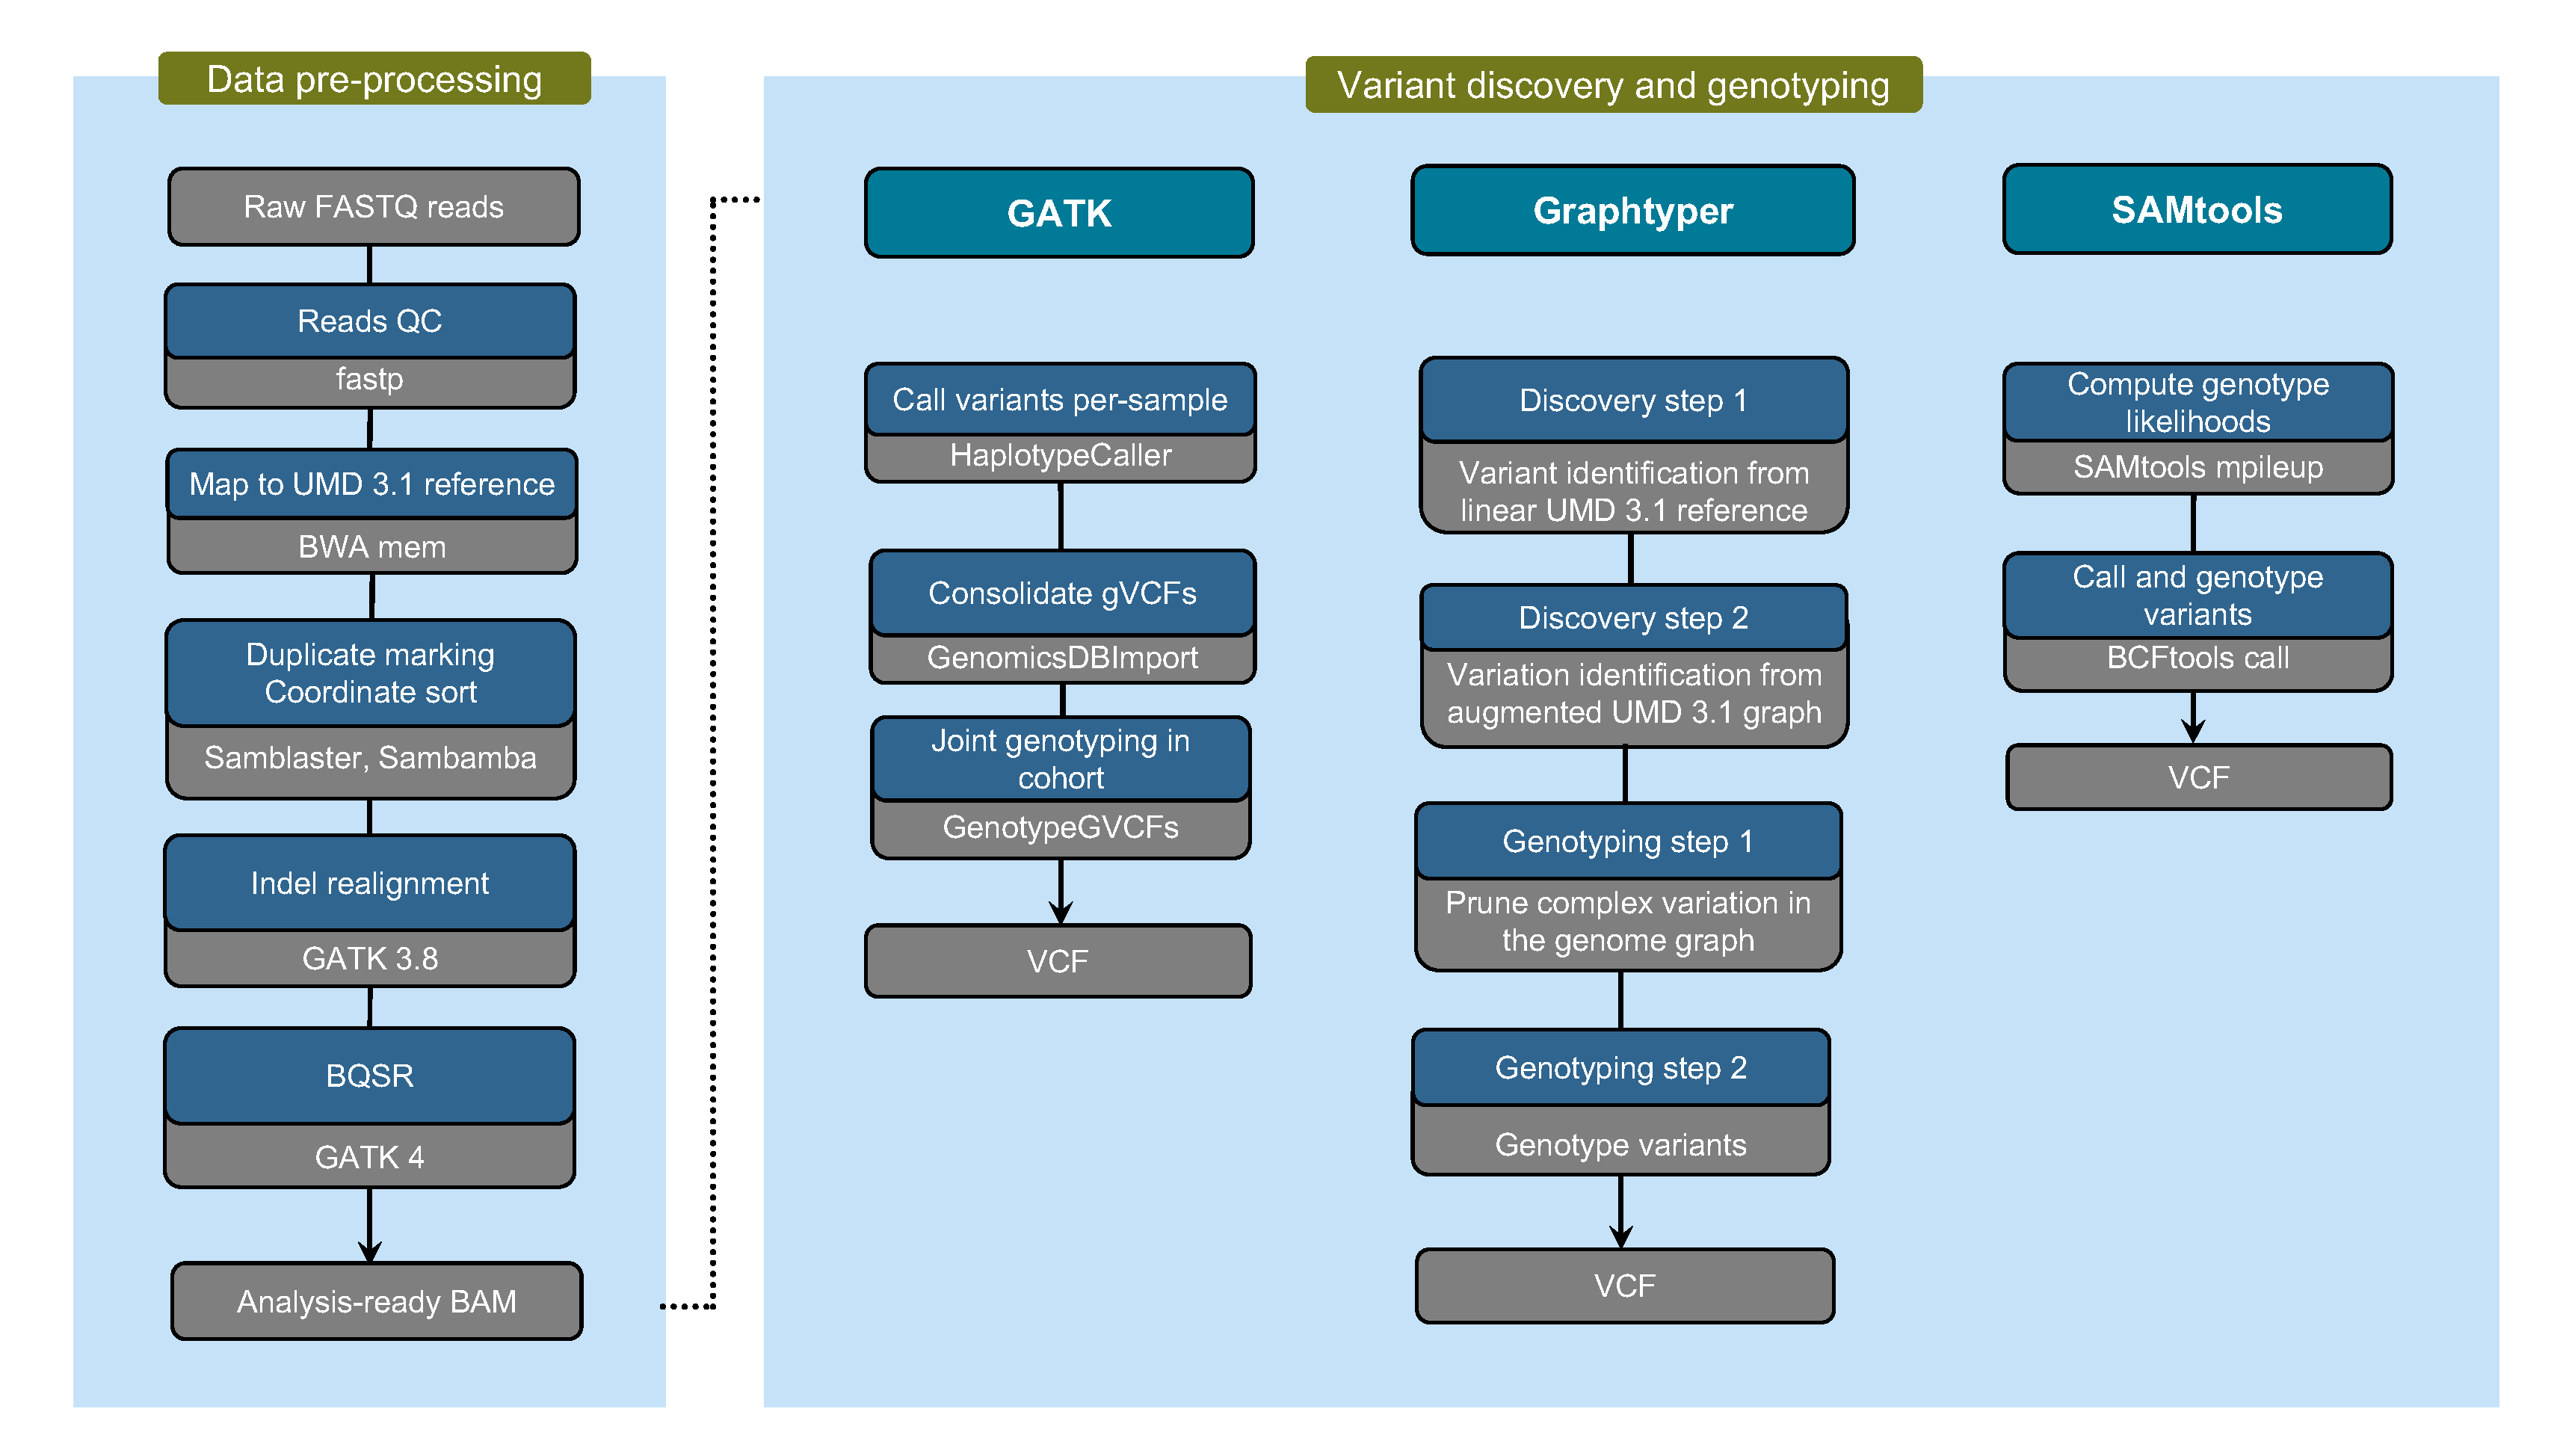
\includegraphics[width=\textwidth]{paper1/main_figure/Figure1.pdf}
    \caption[Scheme of the compared genotyping pipelines]{\textbf{Schematic representation of the three sequence variant discovery and genotyping methods evaluated.} \\
    \small{According to the best practice recommendations for sequence variant discovery using \emph{GATK}, the VQSR module should be applied to distinguish between true and false positive variants. Because this approach requires a truth set of variants, which is not (publicly) available for cattle, the VQSR module was not considered in our evaluation}}
    \label{fig:loca}
\end{figure}

\subsection*{Sequence variant discovery and genotyping}

Polymorphic  sites  (SNPs,  indels)  were  discovered  and  genotyped in the 49 animals using either \emph{GATK} (version 4), \emph{Graphtyper} (version  1.3)  or  \emph{SAMtools} (version  1.8). All software programs were run using default parameters and  workflow  descriptions  for  variant  discovery  (Fig. \ref{fig:loca} and  also  see \nameref{chap2:met}). Only autosomal sequence variants were considered  to  evaluate  the  accuracy  and  sensitivity  of sequence  variant genotyping. Because variant filtering has a strong impact on the accuracy and sensitivity of sequence variant genotyping \citep{carson2014effective,jun2015efficient}, we evaluated both  the  raw  variants  that  were  detected  using  default  parameters  for  variant  discovery  (Fig. \ref{fig:loca})  and  variants  that  remained  after  applying  filtering  criteria  that  are  commonly  used  but  may  differ  slightly  between  different software tools. Note that \emph{GATK} was run by using the suggested filtering parameters, when application of Variant Quality Score Recalibration (\emph{VQSR}) is not possible.

Using default parameters for variant discovery for each of the software programs evaluated, 21,140,196, 20,262,913, and 20,668,459 polymorphic sites were discovered using \emph{GATK}, \emph{Graphtyper} and \emph{SAMtools}, respectively (Table \ref{tab:varcount}). The vast majority (86.79, 89.42 and 85.11\%) of the detected variants were biallelic SNPs. Of the 18,594,182, 18,120,724 and 17,592,038 SNPs detected using \emph{GATK},  \emph{Graphtyper} and \emph{SAMtools}, respectively, 7.46, 8.31 and 5.02\% were novel, i.e., they were not among the 102,091,847 polymorphic sites of the most recent version (150) of the Bovine dbSNP database. The Ti/Tv ratio of the detected SNPs was equal to 2.09, 2.07 and 2.05 using \emph{GATK}, \emph{Graphtyper} and \emph{SAMtool}s, respectively. Using \emph{GATK} revealed four times more multiallelic SNPs (246,220) than either \emph{SAMtools} or \emph{Graphtyper}.

\begin{landscape}

    \begin{table}
        \vspace{10mm} 
        \centering
        \caption[Number of different types of autosomal sequence variants]{\textbf{Number of different types of autosomal sequence variants} detected in 49 Original Braunvieh cattle using three sequence variant genotyping methods (Full) and subsequent variant filtration based on commonly used criteria (Filtered).}
        \vspace{10mm}
        \arrayrulecolor{black}
        \begin{tabular}{|l|l|l|l|l|l|l|} 
        \cline{2-7}
        \multicolumn{1}{l!{\color{black}\vrule}}{~} & \multicolumn{3}{c|}{\multirow{2}{*}{Full\textit{}}}                                                                                                                                                                                      & \multicolumn{3}{c|}{\multirow{2}{*}{Filtered\textit{}}}                                                                                                                                                                                   \\
        \multicolumn{1}{l!{\color{black}\vrule}}{~} & \multicolumn{3}{c|}{}                                                                                                                                                                                                                    & \multicolumn{3}{c|}{}                                                                                                                                                                                                                     \\ 
        \cline{2-7}
        \multicolumn{1}{l!{\color{black}\vrule}}{~} & \multicolumn{1}{c!{\color{black}\vrule}}{\multirow{2}{*}{\textit{GATK}}} & \multicolumn{1}{c!{\color{black}\vrule}}{\multirow{2}{*}{\textit{Graphtyper}}} & \multicolumn{1}{c!{\color{black}\vrule}}{\multirow{2}{*}{\textit{SAMtools}}} & \multicolumn{1}{c!{\color{black}\vrule}}{\multirow{2}{*}{\textit{GATK}}} & \multicolumn{1}{c!{\color{black}\vrule}}{\multirow{2}{*}{\textit{Graphtyper}}} & \multicolumn{1}{c!{\color{black}\vrule}}{\multirow{2}{*}{\textit{SAMtools}}}  \\
        \multicolumn{1}{l!{\color{black}\vrule}}{~} & \multicolumn{1}{c!{\color{black}\vrule}}{}                               & \multicolumn{1}{c!{\color{black}\vrule}}{}                                     & \multicolumn{1}{c!{\color{black}\vrule}}{}                                   & \multicolumn{1}{c!{\color{black}\vrule}}{}                               & \multicolumn{1}{c!{\color{black}\vrule}}{}                                     & \multicolumn{1}{c!{\color{black}\vrule}}{}                                    \\ 
        \arrayrulecolor{black}\hline
        Variants                                    & 21,140,196                                                               & 20,262,913                                                                     & 20,668,459                                                                   & 19,761,679                                                               & 17,679,155                                                                     & 18,871,549                                                                    \\ 
        \arrayrulecolor{black}\hline
        \multicolumn{7}{|l|}{~}                                                                                                                                                                                                                                                                                                                                                                                                                                                                                                            \\ 
        \hline
        SNPs                                        & 18,594,182                                                               & 18,120,724                                                                     & 17,592,038                                                                   & 17,248,593                                                               & 15,777,446                                                                     & 16,272,917                                                                    \\ 
        \hline
        ~ Not in dbSNP                              & 1,387,781~~~~~                                                           & 1,505,586                                                                      & 882,575                                                                      & 867,838                                                                  & 564,326                                                                        & 570,901                                                                       \\ 
        \hline
        ~ Biallelic                                 & 18,347,962                                                               & 18,053,396                                                                     & 17,528,249                                                                   & 17,111,806                                                               & 15,730,153                                                                     & 16,218,714                                                                    \\ 
        \hline
        ~ Multi-allelic                             & 246,220                                                                  & 67,328                                                                         & 63,789                                                                       & 136,787                                                                  & 47,293                                                                         & 54,203                                                                        \\ 
        \hline
        ~ Ti/Tv ratio                               & 2.09                                                                     & 2.07                                                                           & 2.05                                                                         & 2.17                                                                     & 2.18                                                                           & 2.16                                                                          \\ 
        \hline
        \multicolumn{7}{|l|}{SNP array (\%)}                                                                                                                                                                                                                                                                                                                                                                                                                                                                                               \\ 
        \hline
        ~~ BovineHD                                 & 99.46                                                                    & 99.61                                                                          & 99.32                                                                        & 99.21                                                                    & 98.79                                                                          & 98.85                                                                         \\ 
        \hline
        ~~ Bovine SNP50                             & 99.14                                                                    & 99.26                                                                          & 99.12                                                                        & 98.91                                                                    & 98.87                                                                          & 98.90                                                                         \\ 
        \hline
        \multicolumn{7}{|l|}{~}                                                                                                                                                                                                                                                                                                                                                                                                                                                                                                            \\ 
        \hline
        Indels                                      & 2,478,489                                                                & 2,044,585                                                                      & 3,076,421                                                                    & 2,445,766                                                                & 1,826,808                                                                      & 2,598,632                                                                     \\ 
        \hline
        ~ Not in dbSNP                              & 663,831                                                                  & 596,137                                                                        & 1,279,162                                                                    & 639,219                                                                  & 456,752                                                                        & 979,291                                                                       \\ 
        \hline
        ~ Biallelic                                 & 2,166,352                                                                & 1,753,391                                                                      & 2,704,413                                                                    & 2,133,840                                                                & 1,571,195                                                                      & 2,310,386                                                                     \\ 
        \hline
        ~ Multi-allelic                             & 312,137                                                                  & 291,194                                                                        & 372,008                                                                      & 311,926                                                                  & 255,613                                                                        & 288,246                                                                       \\ 
        \hline
        ~ Insertion/Deletion                        & 0.88                                                                     & 0.88                                                                           & 1                                                                            & 0.88                                                                     & 0.88                                                                           & 0.99                                                                          \\ 
        \hline
        \multicolumn{7}{|l|}{~}  \\
        \hline
        Complex variation                           & 67,525                                                                   & 97,604                                                                         & 0                                                                            & 67,320                                                                   & 74,901                                                                         & 0                                                                             \\
        \hline
        \end{tabular}
        \label{tab:varcount}
    \end{table}
\end{landscape}

\newpage

We identified 2,478,489, 2,044,585, and 3,076,421 indels using \emph{GATK}, \emph{Graphtyper}, and \emph{SAMtools}, respectively, and 26.78\%, 29.15\%, and 41.75\% of them were novel. 
\emph{SAMtools} revealed the largest number and highest proportion (14.9\%) of indels. 
Between 12 and 14\% of the detected indels were multiallelic. 
While \emph{Graphtyper} and \emph{GATK} identified more (12\%) deletions than insertions, the proportions were almost the same using \emph{SAMtools}.

On average, each Original Braunvieh cattle carried between 7 and 8 million variants that differed from the UMD3.1 reference genome. 
Of these, between 2.4 and 2.6 million SNPs were homozygous for the alternate allele, between 3.8 and 4.7 million SNPs were heterozygous and between 0.7 and 1 million were indels (Table \ref{tab:varhet}). An intersection of 15,901,526 biallelic SNPs was common to all sequence-variant discovery tools evaluated Fig \ref{fig:varoverlap}a, i.e., between 85.51 and 90.39\% of the detected SNPs of each tool, and 466,029 (2.93\%, Ti/Tv: 1.81) of them were novel, i.e., they were not present in dbSNP 150. 
The Ti/Tv-ratio of the common SNPs was 2.22. 
\emph{SAMtools} had the largest number of SNPs in common with the other two tools (90.39\%). The number of private SNPs, i.e., SNPs that were detected by one but not the other tools was largest for \emph{GATK} and smallest for \emph{Graphtyper}.

In total, 1,299,467 biallelic indels Fig \ref{fig:varoverlap}b were common to all evaluated tools and 98,931 (13.13\%) of these were novel, 
i.e., they were not present in dbSNP 150. The intersection among the three tools was considerably smaller for indels than for SNPs. 
\emph{Graphtyper} had the highest proportion of indels in common with the other tools (74.11\%). 
\emph{SAMtools} discovered the largest number (2,704,413) of biallelic indels and most of them (41.26\%) were not detected using either \emph{GATK} or \emph{Graphtyper}. 
\emph{GATK} (21.2\%) and \emph{Graphtyper} (12.38\%) discovered fewer private indels than \emph{SAMtools}.

\newpage

\begin{landscape}
\begin{table}
    \centering
    \caption[Average number of autosomal variants]{\textbf{Average number of autosomal variants} identified per animal using three sequence variant genotyping methods}
    \vspace{10 mm}
    \begin{tabular}{|l|l|l|l|l|l|l|} 
    \cline{2-7}
    \multicolumn{1}{l|}{}  & \multicolumn{3}{c|}{\multirow{2}{*}{Full}}              & \multicolumn{3}{c|}{\multirow{2}{*}{Filtered}}           \\
    \multicolumn{1}{l|}{}  & \multicolumn{3}{l|}{}                                   & \multicolumn{3}{l|}{}                                    \\ 
    \cline{2-7}
    \multicolumn{1}{l|}{}  & \textit{GATK} & \textit{Graphtyper} & \textit{SAMtools} & \textit{GATK} & \textit{Graphtype}r & \textit{SAMtools}  \\ 
    \hline
    Total biallelic SNPs   & 6,324,455     & 7,384,058           & 6,617,948         & 6,105,674     & 6,533,711           & 6,564,229          \\ 
    \hline
    Heterozygous           & 3,890,351     & 4,758,297           & 4,187,882         & 3,744,336     & 4,074,011           & 4,147,033          \\ 
    \hline
    Homozygous ALT         & 2,434,104     & 2,625,761           & 2,430,066         & 2,361,338     & 2,459,700           & 2,417,196          \\ 
    \hline
    Ti/Tv                  & 2.17          & 2.13                & 2.11              & 2.2           & 2.14                & 2.13               \\ 
    \hline
    Total biallelic indels & 693,697       & 767,261             & 1,007,420         & 691,765       & 697,637             & 960,218            \\ 
    \hline
    Heterozygous           & 390,495 s      & 441,172             & 616,981           & 388,622       & 391,856             & 593,417            \\ 
    \hline
    Homozygous ALT         & 303,202       & 326,089             & 390,439           & 303,143       & 305,781             & 366,801            \\ 
    \hline
    Singletons             & 49,166        & 23,406              & 32,810            & 41,408        & 17,999              & 32,398             \\
    \hline
    \end{tabular}
    \label{tab:varhet}
    \end{table}
    \singlespacing
    \small{The number of variants is presented for the three tools evaluated before (Full) and after (Filtered) applying recommended filters to identify and exclude low quality variants}
\end{landscape}

\newpage
\begin{figure}[!htb]
    \centering
    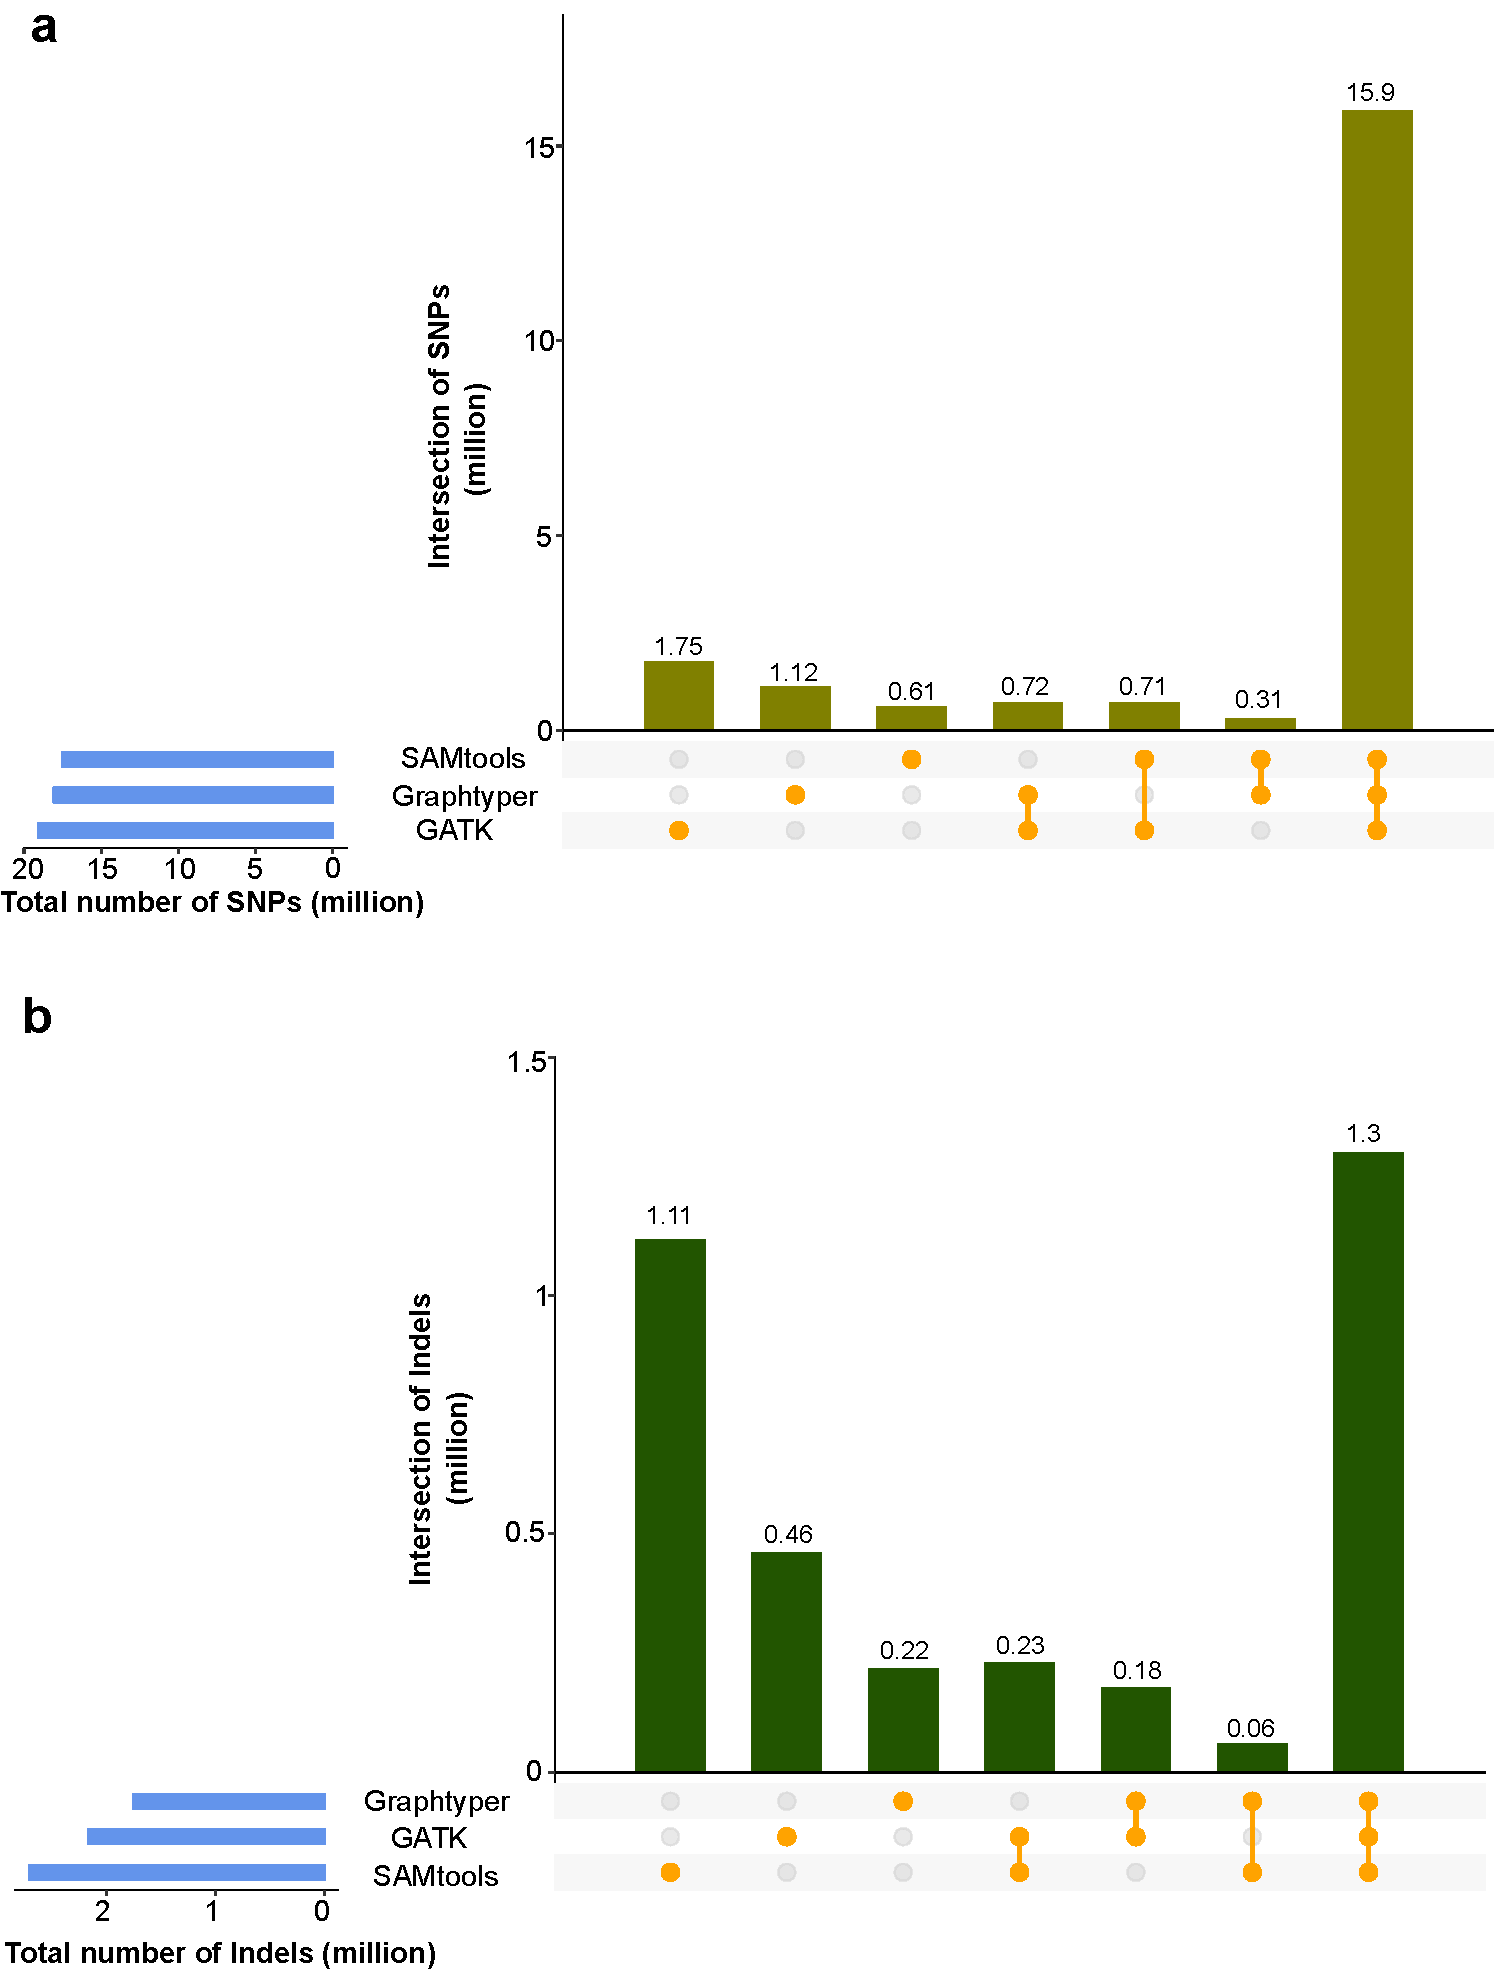
\includegraphics[width=\textwidth]{paper1/main_figure/Figure2.pdf}
    \caption[Number of biallelic variants]{\textbf{Number of biallelic SNPs (a) and indels (b)} identified in 49 Original Braunvieh cattle using three sequence variant genotyping methods. Blue horizontal bars represent the total number of sites discovered for each method. Vertical bars indicate private and common variants detected by the methods evaluated}
    \label{fig:varoverlap}
\end{figure}

\newpage

\subsection*{Sequence variant genotyping using \emph{Graphtyper} is accurate}

The 49 sequenced animals were also genotyped using either the Illumina BovineHD or the Illumina BovineSNP50 Bead chip. 
Genotype concordance, non-reference sensitivity and non-reference discrepancy were calculated using array-called and 
sequence variant genotypes at corresponding positions. Genotype concordance is a measure of the proportion of variants that have
identical genotypes on the microarray and in whole-genome sequencing data. 
Non-reference sensitivity is the proportion of microarray-derived variants that were also detected in the sequencing data. 
Non-reference discrepancy reflects the proportion of sequence variants that have genotypes that differ from the microarray-derived genotypes [for more details on how the different metrics were calculated (see \ref{supp_mat:22})]. 
All metrics were calculated both for raw and filtered variants either before or after applying the algorithm implemented in the \emph{Beagle} software for haplotype phasing and imputation.

In the raw data, the proportion of missing non-reference sites was 1.90\%, 0.56\%, and 0.47\% using \emph{GATK}, \emph{Graphtyper}, and \emph{SAMtools}, respectively.
The genotype concordance between the sequence- and microarray-derived genotypes was higher (\emph{P} $<$ 0.005) when \emph{Graphtyper} (97.72\%) was used than when either \emph{SAMtools} (97.68\%) or \emph{GATK} (95.99\%) was used (Table \ref{tab:varcomp}). 
For the three tools evaluated, the genotype concordance was higher at homozygous than heterozygous sites, particularly in animals that were sequenced at low depth (see \ref{supp_mat:23}).
In order to take the variable proportions of missing genotypes in the sequence variants into account, we calculated non-reference sensitivity and non-reference discrepancy. 
Non-reference sensitivity was almost identical using \emph{Graphtyper} (98.26\%) and \emph{SAMtools} (98.21\%). 
However, non-reference sensitivity was clearly lower using \emph{GATK} (93.81\%, \emph{P} $<$ 0.001). 
Non-reference discrepancy was lower using \emph{Graphtyper} (3.53\%) than using either \emph{SAMtools} (3.6\%, \emph{P} $=$ 0.003) or \emph{GATK} (6.35\%, \emph{P} $<$ 0.001).

\begin{landscape}
    \begin{table}
        \centering
        \caption[Comparisons between array-called and sequence variant genotypes]{\textbf{Comparisons between array-called and sequence variant genotypes.}}
        \small
        \arrayrulecolor{black}
        \begin{tabular}{|l|l|l|l|l|l|l|l|l|l|l|l|l|} 
        \cline{2-13}
        \multicolumn{1}{l|}{\multirow{3}{*}{~}} & \multicolumn{4}{l|}{Genotype concordance}                         & \multicolumn{4}{l|}{Non-reference sensitivity}                    & \multicolumn{4}{l|}{Non-reference discrepancy}                 \\ 
        \cline{2-13}
        \multicolumn{1}{l|}{}                   & \multicolumn{2}{l|}{full}       & \multicolumn{2}{l|}{filtered}   & \multicolumn{2}{l|}{full}       & \multicolumn{2}{l|}{filtered}   & \multicolumn{2}{l|}{full}     & \multicolumn{2}{l|}{filtered}  \\ 
        \cline{2-13}
        \multicolumn{1}{l|}{}                   & raw            & imp            & raw            & imp            & raw            & imp            & raw            & imp            & raw           & imp           & raw           & imp            \\ 
        \arrayrulecolor{black}\cline{1-1}\arrayrulecolor{black}\cline{2-13}
        \textit{GATK}                           & 95.99***       & 99.32***       & 96.02***       & 99.39***       & 93.81***       & \textit{99.36} & 93.67***       & \textit{99.15} & 6.35***       & 1.05***       & 6.3***        & 0.95***        \\ 
        \hline
        \textit{Graphtyper}                     & \textit{97.71} & \textit{99.46} & \textit{97.75} & \textit{99.52} & \textit{98.26} & 99.35          & \textit{97.91} & 99.00***       & \textit{3.53} & \textit{0.83} & \textit{3.47} & \textit{0.73}  \\ 
        \hline
        \textit{SAMtools}                       & 97.68***       & 99.24***       & 97.7*          & 99.29***       & 98.21          & 99.35          & 97.53***       & 98.67***       & 3.6**         & 1.17***       & 3.56**        & 1.09***        \\
        \hline
        \end{tabular}
        \label{tab:varcomp}
        \end{table}
        \singlespacing
        \small{Genotype concordance, non-reference sensitivity and non-reference discrepancy (in percentage) was calculated between 
        the genotypes from the Bovine SNP Bead chip and sequence–derived genotypes for 49 Original Braunvieh cattle considering either the raw or imputed (imp) sequence variant 
        genotypes before (full) and after (filtered) variants were filtered based on commonly used criteria. 
        Asterisks denote a significant difference (* \emph{P} $<$ 0.05, ** \emph{P} $<$ 0.01, *** \emph{P} $<$ 0.001) with the best value (italic) for a respective parameter.}

\end{landscape}


Next, we analysed the proportion of opposing homozygous genotypes for SNPs and indels in nine sire-son pairs that were included among the sequenced animals (Table \ref{tab:mendel}). 
We observed that SNPs that were discovered using either \emph{Graphtyper} or \emph{SAMtools} had almost a similar proportion of genotypes with Mendelian inconsistencies in the full and filtered datasets, whereas the values were two times higher using \emph{GATK}. 
The proportion of opposing homozygous genotypes was higher for indels than SNPs for all the tools evaluated. 
However, in the full and filtered datasets, it was lower when \emph{Graphtyper} was used than when either \emph{GATK} or \emph{SAMtools} was used. Using filtering parameters that are commonly applied for the three evaluated tools (see \nameref{chap2:met}), 
we excluded 1,378,517 (6.52\%, Ti/Tv 1.24), 2,583,758 (12.75\%, Ti/Tv 1.47) and 1,796,910 (8.69\%, Ti/Tv 1.36) variants due to low mapping or genotyping quality from the \emph{GATK}, \emph{Graphtyper}, and \emph{SAMtools} datasets, respectively. 
The genotype concordance between sequence- and microarray-derived genotypes was slightly higher for the filtered than the raw genotypes, but the non-reference sensitivity was lower for the filtered than the raw genotypes, which indicates that the filtering step also removed some true variant sites from the raw data (Table \ref{tab:varcomp}). 
The filtering step had almost no effect on the proportion of Mendelian inconsistencies detected in the nine sire-son pairs (Table \ref{tab:mendel}).

\begin{table}
            \begin{center}
            \caption[Proportions of opposing homozygous genotypes observed in nine sire-son pairs]{\textbf{Proportions of opposing homozygous genotypes observed in nine sire-son pairs}}
            \small
            \begin{tabular}{|l|l|l|l|l|l|l|l|l|} 
            \cline{2-9}
            \multicolumn{1}{l!{\color{black}\vrule}}{~} & \multicolumn{4}{l|}{SNPs}                                     & \multicolumn{4}{l|}{indels}                                    \\ 
            \cline{2-9}
            \multicolumn{1}{l|}{~}                      & \multicolumn{2}{l|}{full}     & \multicolumn{2}{l|}{filtered} & \multicolumn{2}{l|}{full}     & \multicolumn{2}{l|}{filtered}  \\ 
            \cline{2-9}
            \multicolumn{1}{l|}{~}                      & raw           & imp           & raw           & imp           & raw           & imp           & raw           & imp            \\ 
            \hline
            \textit{Bovine HD SNP array}                & \multicolumn{8}{l|}{\textit{0.001}}                                                                                            \\ 
            \hline
            \textit{GATK}                               & 0.73*         & 0.15*         & 0.72*         & 0.13*         & 0.98*         & 0.24*         & 0.99*         & 0.21*          \\ 
            \hline
            \textit{Graphtyper}                         & 0.36          & \textit{0.11} & 0.36          & \textit{0.11} & \textit{0.54} & \textit{0.13} & \textit{0.54} & \textit{0.13}  \\ 
            \hline
            \textit{SAMtools}                           & \textit{0.33} & 0.28*         & \textit{0.32} & 0.25*         & 0.67          & 0.54*         & 0.61          & 0.57*          \\
            \hline
            \end{tabular}
            \label{tab:mendel}
            \end{center}
            \singlespacing
            \small{The ratio (in percentage) was calculated using autosomal sequence variants considering either 
            the raw or imputed (imp) sequence variant genotypes before (full) and after (filtered) variants were filtered based on commonly used criteria. 
            Asterisks denote significant differences (* \emph{P} $\leq$ 0.05, ** \emph{P} $\leq$ 0.01, *** \emph{P} $\leq$ 0.001) with the best value (italic) for a respective parameter.}

\end{table}

\subsubsection*{\emph{Beagle} genotype refinement improved genotype quality}

We used the \emph{Beagle} software to refine the primary genotype calls and infer missing genotypes in the raw and filtered datasets. 
Following imputation, the quality of the sequence variant genotypes increased for all evaluated tools particularly for the individuals that had a sequencing coverage less than 12-fold (Fig. \ref{fig:varimpute}). 
The largest increase in the concordance metrics was observed for the sequence variants that were obtained using \emph{GATK} (Tables \ref{tab:varcomp} and \ref{tab:mendel}). 
Following imputation, the variants identified using \emph{Graphtyper} had a significantly higher quality (\emph{P $<$} 0.05) for eight out of the ten metrics evaluated.

The quality of the sequence variant genotypes, particularly before \emph{Beagle} genotype phasing and imputation, was influenced by the variable depth of coverage for the 49 sequenced samples of our study (Fig. \ref{fig:varimpute}). 
When we restricted the evaluations to 31 samples that had an average sequencing depth above 12-fold, the three tools performed almost identically (see \ref{supp_mat:24}). 
However, the performance of \emph{Graphtyper} was significantly (\emph{P $<$} 0.05) higher for 12 (out of the total 20) metrics than either that of \emph{GATK} or \emph{SAMtools}. 
When 18 samples with an average sequencing depth lower than 12-fold were considered, the differences observed in the three metrics were more pronounced between the three tools. 
In samples with a low sequencing coverage, \emph{Graphtyper} performed significantly (\emph{P $<$} 0.05) better than either \emph{GATK} or \emph{SAMtools} for all concordance metrics both before and after filtering and \emph{Beagle} imputation, except for the non-reference sensitivity.

\begin{figure}[!htb]
    \centering
    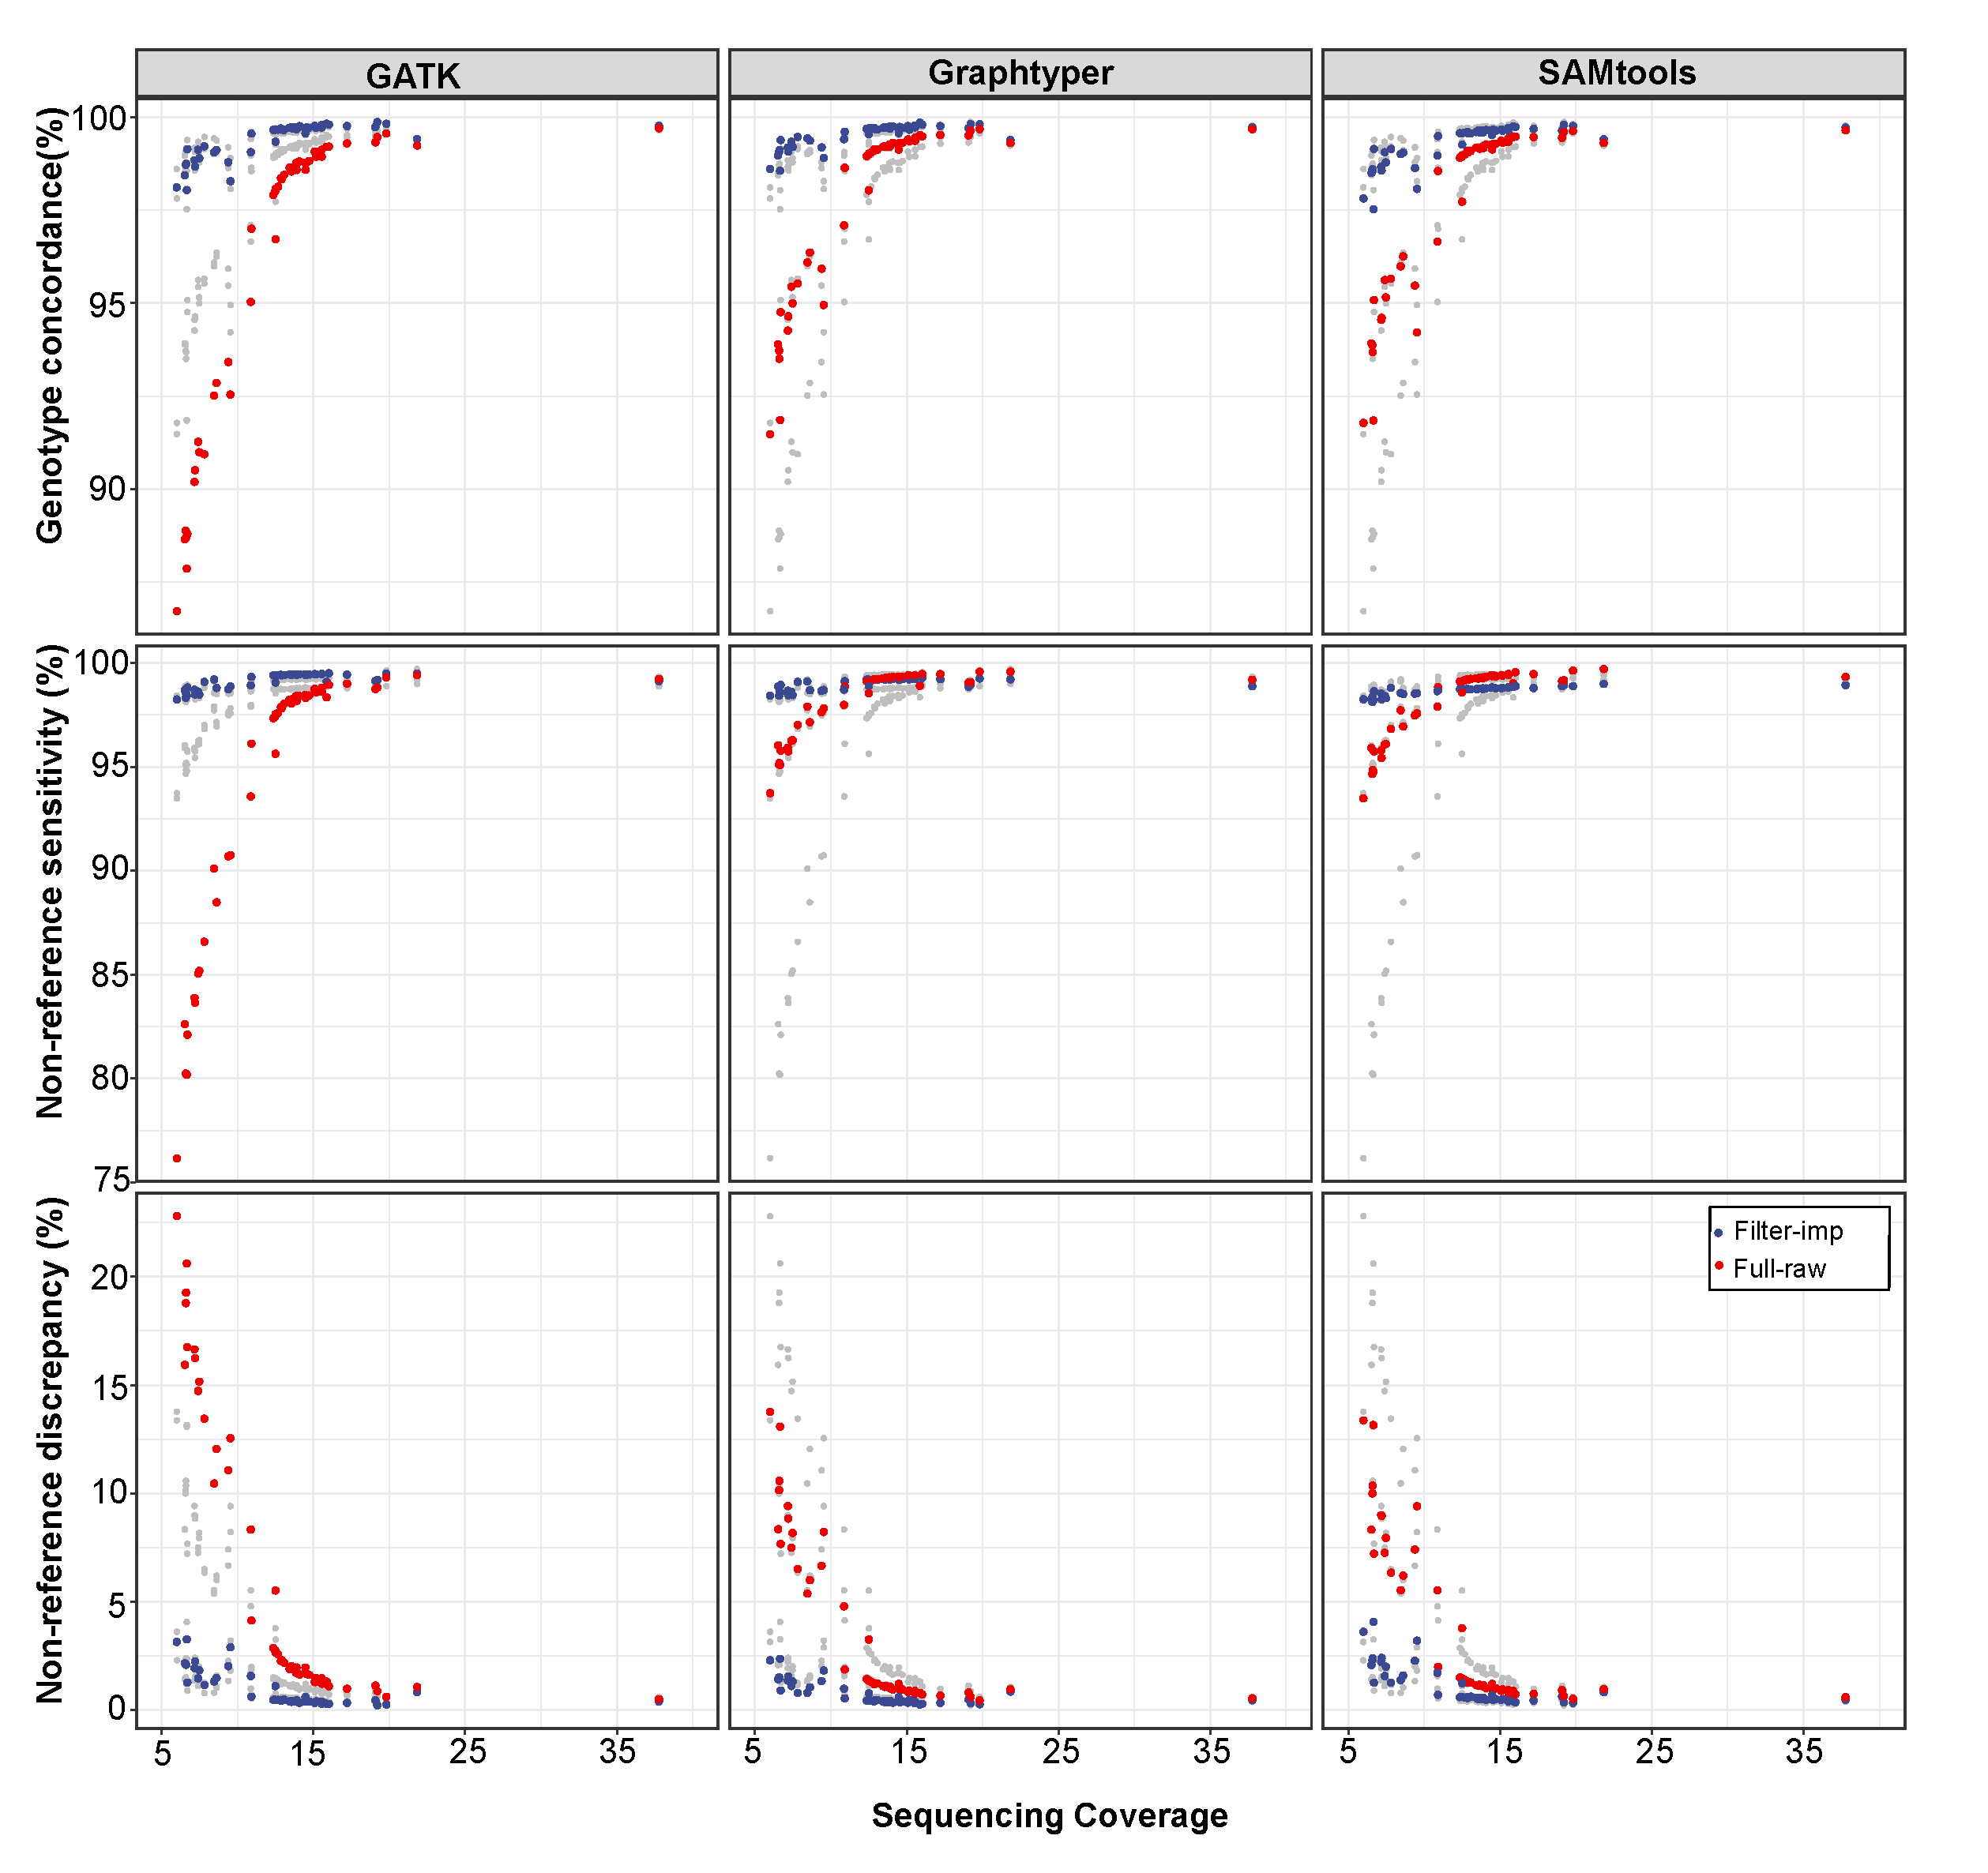
\includegraphics[width=\textwidth]{paper1/main_figure/Figure3.pdf}
    \caption[Accuracy and sensitivity of sequence variant genotyping at different sequencing depths]{\textbf{Accuracy and sensitivity of sequence variant genotyping at different sequencing depths.} Genotype concordance, non-reference sensitivity and non-reference discrepancy were calculated for 49 Original Braunvieh cattle considering either raw (red) or filtered and imputed (blue) sequence variant genotypes. The grey points represent overlays of the results from the other methods}
    \label{fig:varimpute}
\end{figure}

\subsection*{Computing requirements}

The multi-sample sequence variant genotyping pipelines that were implemented using either \emph{GATK} or \emph{SAMtools} were run separately for each chromosome in a single-threading mode. 
The \emph{SAMtools mpileup} module took between 3.07 and 11.4 CPU hours and required between 0.12 and 0.25 gigabytes (GB) peak random-access memory (RAM) per chromosome. 
To genotype 20,668,459 sequence variants in 49 animals, \emph{SAMtools} mpileup required 192 CPU hours (Fig. \ref{fig:varresource}).

\begin{figure}[!htb]
    \centering
    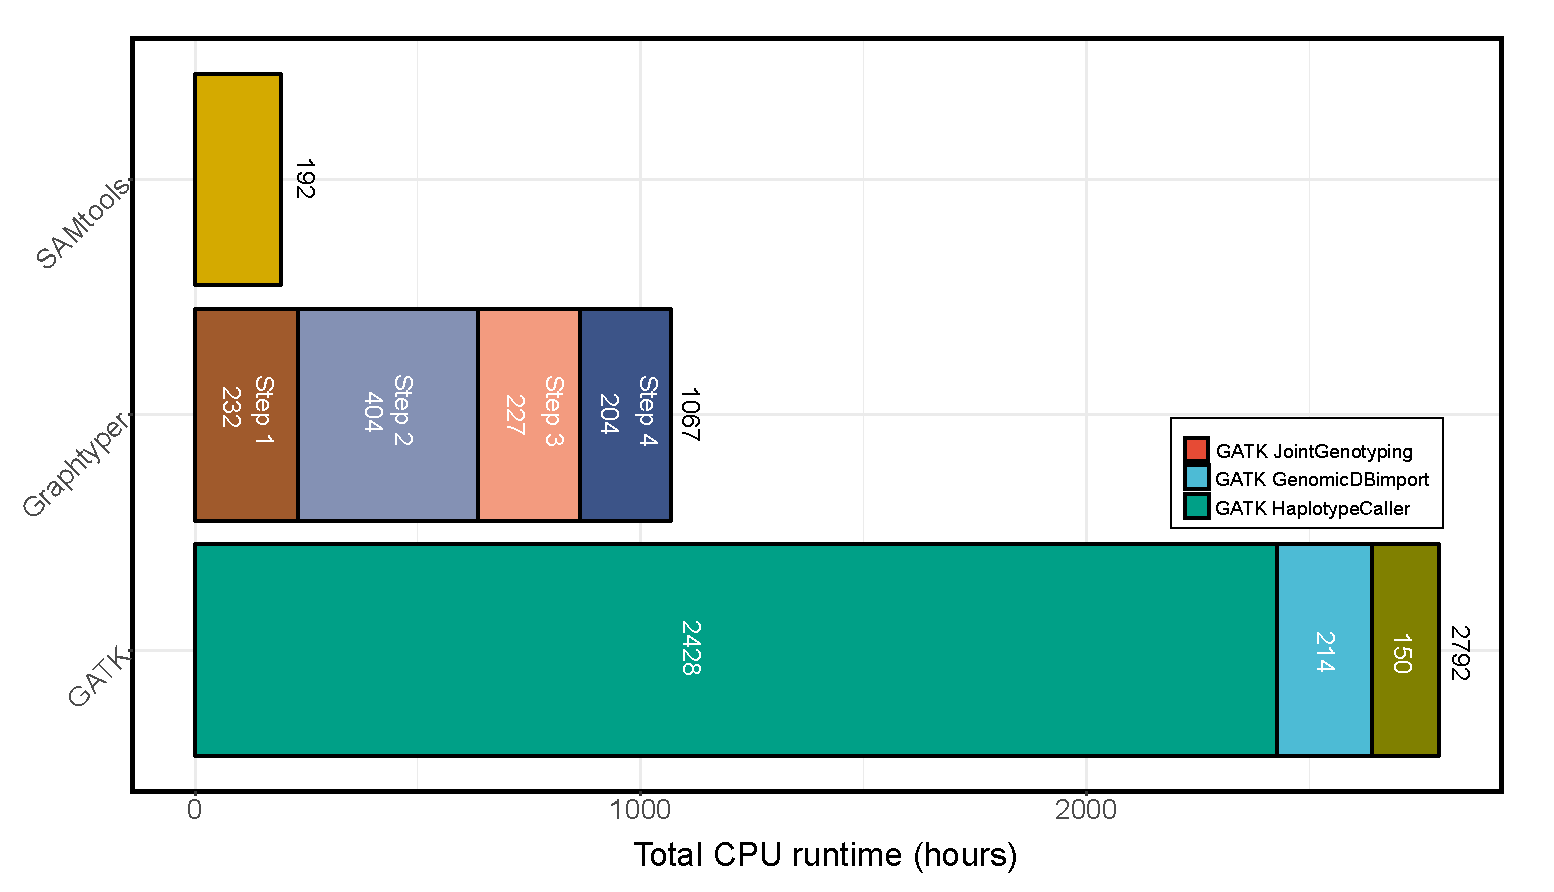
\includegraphics[width=\textwidth]{paper1/main_figure/Figure4.pdf}
    \caption[Computing time required for genotyping]{\textbf{Computing time required to genotype all autosomal sequence variants in 49 Original Braunvieh cattle.} The runtime of \emph{GATK} and \emph{Graphtyper }is shown for the different steps (see Fig. \ref{fig:loca} for more details)}
    \label{fig:varresource}
\end{figure}

For \emph{GATK}, we submitted 1421 parallel jobs of the \emph{HaplotypeCaller} module (i.e., one job for each animal and chromosome) that required between 3.9 and 12.3 GB RAM and between 0.36 and 11 CPU hours to complete.
To process 29 chromosomes in 49 samples, the \emph{HaploytpeCaller} module required 2428 CPU hours. 
Subsequently, we ran the \emph{GATK GenomicsDBImport} module, which required between 7.98 and 20.88 GB RAM and between 2.81 and 19.31 CPU hours per chromosome. 
\emph{GATK Joint Genotyping} required between 4.33 and 17.32 GB of RAM and between 1.81 and 14.01 h per chromosome. 
To genotype 21,140,196 polymorphic sequence variants in 49 animals, the \emph{GATK} pipeline required 2792 CPU hours (Fig. \ref{fig:varresource}).

The \emph{Graphtyper} pipeline including construction of the variation graph and genotyping of sequence variants was run in parallel for 2538 non-overlapping segments of 1 million bp as recommended by \citet{eggertsson2017graphtyper}. 
The peak RAM required by \emph{Graphtyper} was between 1 and 3 GB per segment. 
Twelve segments, for which \emph{Graphtyper} either ran out of memory or did not finish within the allocated time, were subdivided into smaller segments of 10 kb and subsequently re-run (\ref{supp_mat:25}).
The genotyping of 20,262,913 polymorphic sites in 49 animals using our implementation of the \emph{Graphtyper} pipeline required 1066 CPU hours (Fig. \ref{fig:varresource}).


The computing resources required by \emph{SAMtools} and \emph{GATK} increased linearly with chromosome length. 
The computing time required to genotype sequence variants was highly heterogeneous along the genome using \emph{Graphtyper}. 
The CPU time for a 1-Mb segment ranged from 0.196 to 10.11 h, with an average CPU time of 0.42 h. 
We suspected that flaws in the reference genome might increase the complexity of the variation-aware graph and that the construction of the graph might benefit from an improved assembly. 
To test this hypothesis, we re-mapped the sequencing reads to the recently released new bovine reference genome (ARS-UCD1.2, \url{https://www.ncbi.nlm.nih.gov/assembly/GCF_002263795.1}) and repeated the graph-based sequence variant discovery. 
Indeed, we did observe a decrease in the computing time required to genotype polymorphic sites (particularly at chromosomes 12, 27 and 29) and a more uniform runtime along the genome, which possibly indicates that graph-based variant discovery in cattle will be faster and more accurate with highly contiguous reference sequences (Fig. \ref{fig:varassemb}).


\begin{figure}[!htb]
    \centering
    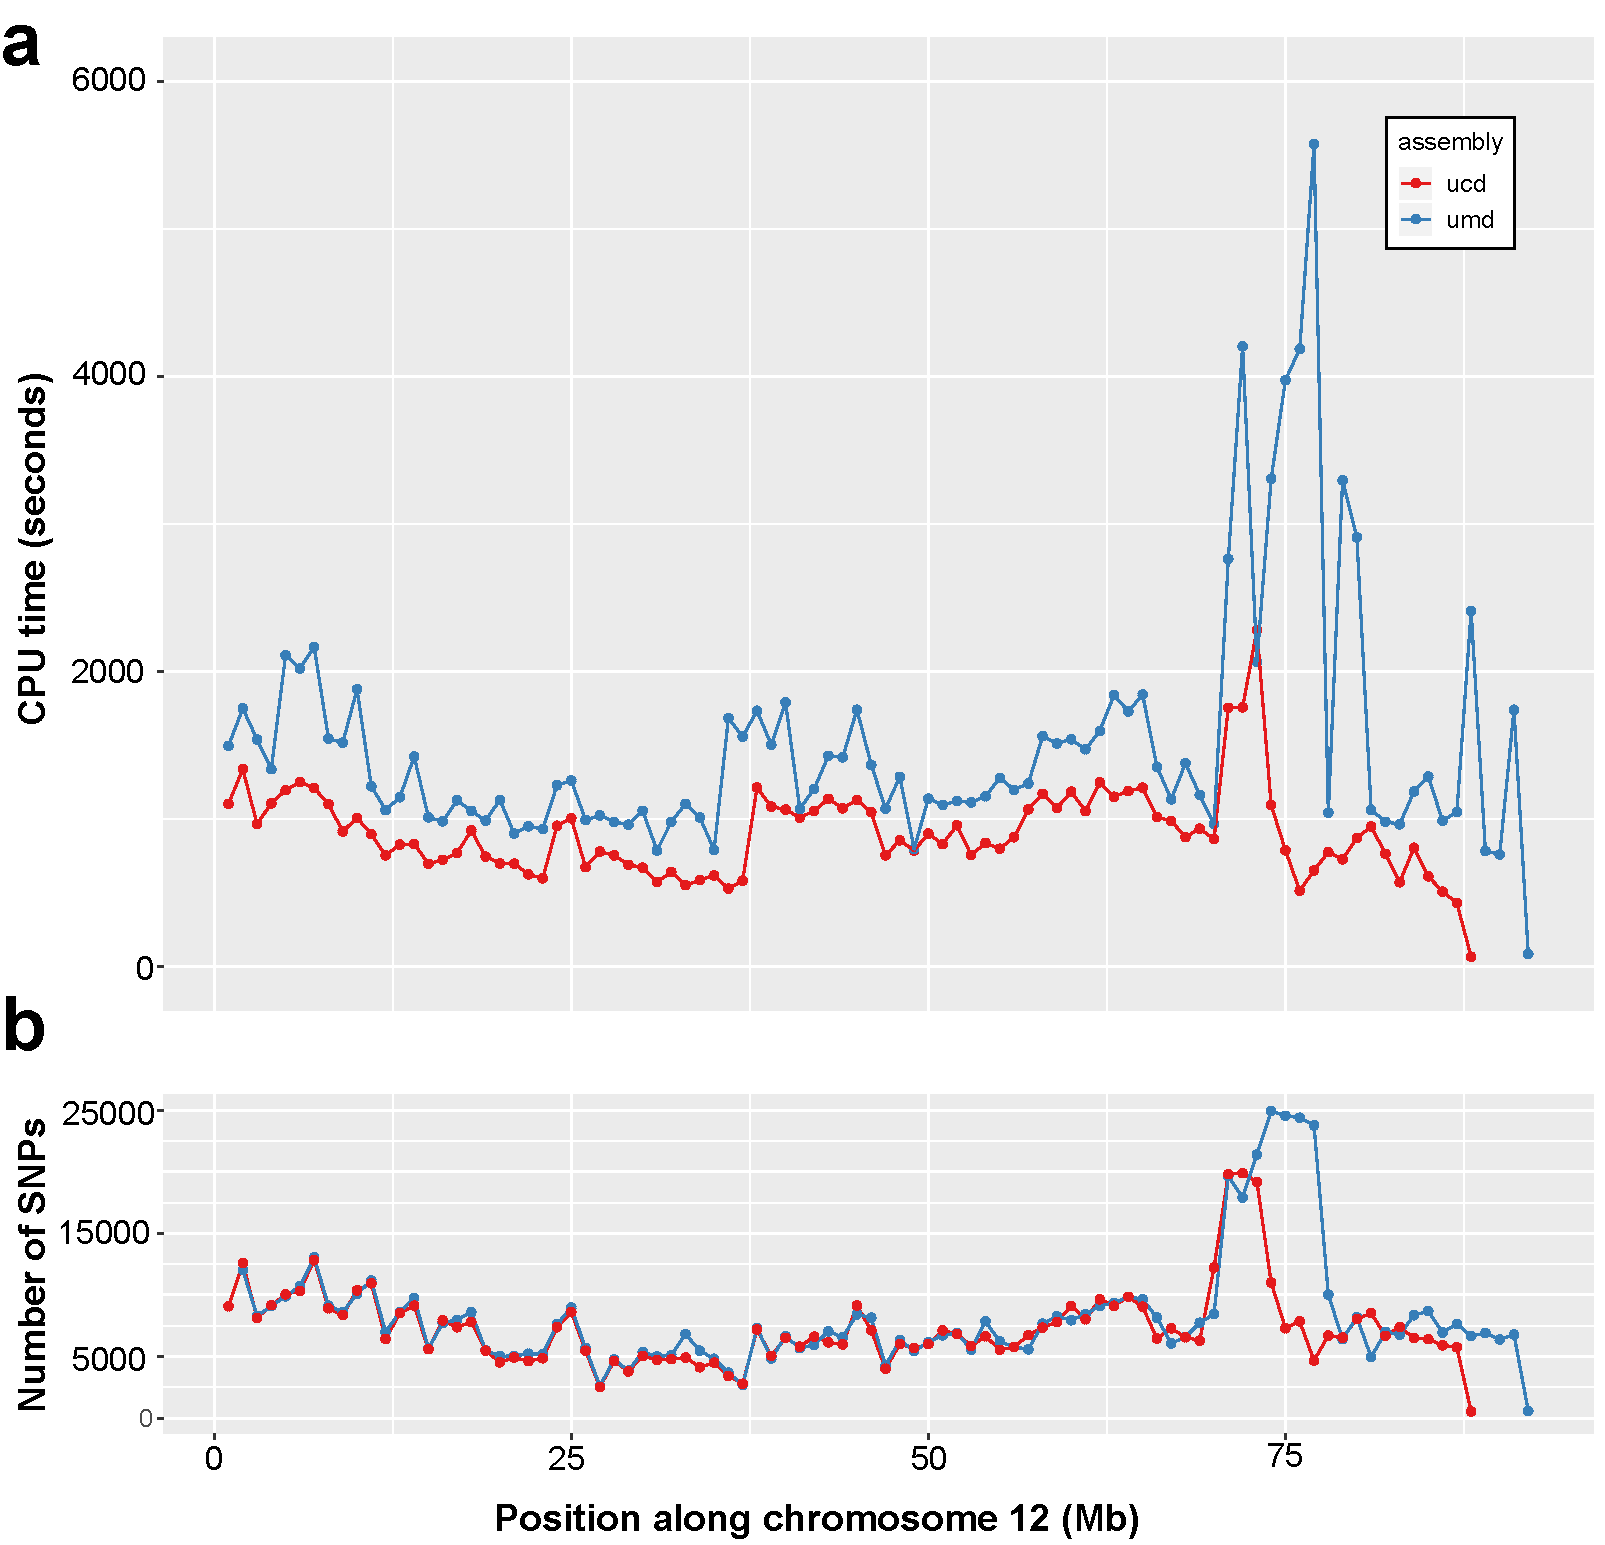
\includegraphics[width=\textwidth]{paper1/main_figure/Figure5.pdf}
    \caption[Sequence variant genotyping on chromosome 12 using \emph{Graphtyper}]{\textbf{Sequence variant genotyping on chromosome 12 using \emph{Graphtyper}.} Computing time required (\textbf{a}) and number of variants discovered (\textbf{b}) for bovine chromosome 12 using \emph{Graphtyper}. 
    Each dot represents an interval of 1 million bp. Blue and red colours represent values for the UMD3.1 and ARS-UCD1.2 versions of the bovine assembly, respectively}
    \label{fig:varassemb}
\end{figure}

\section{Discussion}

We used either \emph{GATK}, \emph{Graphtyper}, or \emph{SAMtools} to discover and genotype polymorphic sequence variants in whole-genome sequencing data of 49 Original Braunvieh cattle that were sequenced at between 6 and 38-fold genome coverage. 
Whereas \emph{SAMtools} and \emph{GATK} discover variants from a linear reference genome, \emph{Graphtyper} locally realigns reads to a variation-aware reference graph that incorporates cohort-specific sequence variants \citep{eggertsson2017graphtyper}. 
Our graph-based variant discovery pipeline that is implemented by using the \emph{Graphtyper} software used the existing bovine reference sequence to construct the genome graph. 
Subsequently, the graph was augmented with variants that were detected from linear alignments of the 49 Original Braunvieh cattle. 
The use of more sophisticated genome graph-based approaches that have been developed very recently facilitates the mapping of raw sequencing reads directly against a genome graph without the need to first align reads towards a linear reference genome \citep{garrison2018variation}. 
Whereas genome graph-based variant discovery has been explored recently in mammalian-sized genomes \citep{dilthey2015improved,rakocevic2019fast,garrison2018variation,sibbesen2018accurate}, our work is the first to apply graph-based sequence variant genotyping in cattle.

In order to evaluate graph-based variant discovery in cattle, we compared accuracy and sensitivity of \emph{Graphtyper} to \emph{GATK}, and \emph{SAMtools} , i.e., two state-of-the-art methods on linear reference genomes that have been evaluated thoroughly in many species including cattle \citep{Jansen2013,baes2014evaluation}. 
We ran each tool with default parameters for variant discovery and applied commonly used or recommended filtration criteria. 
However, our evaluation of the software tools may suffer from ascertainment bias because we relied on SNPs that are included in bovine SNP arrays, i.e., they are located predominantly at genomic regions where variants are easy to identify \citep{li2014toward,malomane2018efficiency,linderman2014analytical}. 
Thus, the global accuracy and sensitivity of sequence variant discovery might be overestimated in our study. 
However, this ascertainment bias is unlikely to affect the relative performance of the methods evaluated.

In 49 Original Braunvieh cattle, sequence variant genotyping was more accurate using \emph{Graphtyper} than either \emph{GATK} or \emph{SAMtools}. Differences in accuracy are small between the three tools, particularly when samples are sequenced at an average coverage higher than 12-fold (see \ref{supp_mat:24}). Yet, \emph{Graphtyper} performed significantly better than \emph{GATK} and \emph{SAMtools} for samples sequenced at medium ($>$ 12-fold) or low($<$ 12-fold)
coverage indicating that genome graph-based variant discovery in cattle is accurate across a wide range of sequencing depths. \emph{GATK} might perform better than observed in our study, when the VQSR module is applied to train the variant filtration algorithm on true and false variants \citep{pirooznia2014validation}. However, to the best of our knowledge, the required sets of true and false variants are not available in cattle. An intersection of variants detected by different sequence variant genotyping software may be considered as a truth set (e.g., \citet{alberto2018convergent}) and compiling such a set is possible using the 49 samples from our study. However, a truth set that has been constructed from the data that are used for evaluation is likely to be depleted for variants that are difficult to discover in the target data set, thus preventing an unbiased evaluation of variant calling \citep{li2018synthetic}. Variants from the 1000 Bull Genomes project \citep{Daetwyler2014,Hayes2019} could potentially serve as a truth/training set. However, variants from the 1000 Bull Genomes project were detected from short read sequencing data using either \emph{GATK} or \emph{SAMtools}, i.e., technologies and software that are part of our evaluation, thus precluding an unbiased comparison of variant discovery between \emph{GATK}, \emph{Graphtyper}, and \emph{SAMtools} \citep{li2018synthetic}. \citet{vander2018best} showed in a subset of samples from the 1000 Bull Genomes project that \emph{GATK VQSR} does not notably improve the concordance between sequence-derived and microarray-called genotypes compared to \emph{GATK} hard filtering. Interestingly, the proportion of opposing homozygous genotypes in sire/offspring pairs was slightly higher in their study using \emph{GATK VQSR} than \emph{GATK} hard-filtering as used by the 1000 Bull Genomes project \citep{vander2018best}. Applying \emph{GATK} VQSR to the variants of our dataset corroborates the findings of \citet{vander2018best} (see \ref{supp_mat:26}). Considering that the quality of the truth/training sets has a strong impact on the capabilities of VQSR (\ref{supp_mat:26}) and that high-confidence variants are currently not publicly available for cattle, we report \emph{GATK} results using the recommended filtering parameters when VQSR is not possible.

Regardless of the method evaluated, we observed heterozygous under-calling in animals that are sequenced at low coverage, i.e., heterozygous variants were erroneously genotyped as homozygous due to an insufficient number of sequencing reads supporting the heterozygous genotype \citep{nielsen2011genotype,sims2014sequencing,fragoso2016imputing,bilton2018linkage}. In agreement with previous studies \citep{Jansen2013,Daetwyler2014}, \emph{Beagle} imputation improved genotype concordance and reduced heterozygous under-calling particularly in individuals that are sequenced at low coverage. After the imputation step, the genotype concordance, non-reference sensitivity, and non-reference discrepancy of the three tools were almost identical, which indicates that genotyping sequence variants from samples with a medium genome coverage is possible at high accuracy (at least for common variants in more accessible regions of the genome) using any of the three tools evaluated and subsequent \emph{Beagle} error correction. While such conclusions have been drawn previously for \emph{SAMtools} and \emph{GATK} \citep{Jansen2013,baes2014evaluation}, our findings demonstrate that the genotype likelihoods estimated from the \emph{Graphtyper} software are also compatible with and benefit from the imputation algorithm implemented in the \emph{Beagle} software. Considering that sequence data are enriched for rare variants that are more difficult to impute than common variants from SNP microarrays \citep{pausch2017evaluation}, the benefits from \emph{Beagle} error correction might be overestimated in our study. An integration of phasing and imputation of missing genotypes directly in a graph-based variant genotyping approach would simplify sequence variant genotyping from variation-aware graphs \citep{rakocevic2019fast,siren2020haplotype,novak2017graph}. Using \emph{Graphtyper} for variant genotyping and \emph{Beagle} for genotype refinement enabled us to genotype sequence variants in 49 Original Braunvieh cattle at a genotypic concordance of 99.52\%, i.e., higher than previously achieved using either \emph{GATK} or \emph{SAMtools} for variant calling in cattle that are sequenced at a similar genome coverage \citep{Jansen2013,Stothard2015,Boussaha2016,Daetwyler2014,baes2014evaluation,stafuzza2017single}; this indicates that graph-based variant discovery might improve sequence variant genotyping. However, applying the filtering criteria that are recommended for \emph{Graphtyper} \citep{eggertsson2017graphtyper} removed more variants from the \emph{Graphtyper} (12.75\%) than from either \emph{GATK} (6.52\%) or \emph{SAMtools} (8.69\%) datasets. It should be mentioned that \emph{GATK} VQSR would remove considerably more variants from the \emph{GATK} dataset than \emph{GATK} hard filtering as applied in our study (see \ref{supp_mat:26}). Fine-tuning of the variant filtering parameters is necessary to further increase the accuracy and sensitivity of sequencing variant genotyping, particularly for \emph{Graphtyper} \citep{carson2014effective,jun2015efficient}. Moreover, the accuracy and sensitivity of graph-based variant discovery may be higher when known variants are considered for the initial construction of the variation graph \citep{eggertsson2017graphtyper}. Indeed, we observed a slight increase in genotype concordance (see \ref{supp_mat:27}) when we used \emph{Graphtyper} to genotype sequence variants from a variation-aware genome-graph that incorporated bovine variants listed in dbSNP 150. However, additional research is required to prioritize a set of variants to augment bovine genome graphs for different cattle breeds \citep{pritt2018forge}.

Using microarray-derived genotypes as a truth set may overestimate the accuracy of sequence variant discovery particularly at variants that are rare or located in less accessible regions of the genome. Moreover, it does not allow assessment of the accuracy and sensitivity of indel discovery because variants other than SNPs are currently not routinely genotyped with commercially available microarrays. Estimating the proportion of opposing homozygous genotypes between parent–offspring pairs may be a useful diagnostic metric to detect sequencing artefacts or flawed genotypes at indels \citep{patel2014struggle}. Our results show that genotypes at indels are more accurate using \emph{Graphtyper} than either \emph{SAMtools} or \emph{GATK} because \emph{Graphtyper} produced less opposing homozygous genotypes at indels in nine sire-son pairs than the other methods both in the raw and filtered datasets. These findings are in line with those reported by \citet{eggertsson2017graphtyper}, who showed that the mapping of the sequencing reads to a variation-aware graph could improve read alignment nearby indels, thus enabling highly accurate sequence variant genotyping also for variants other than SNPs. Recently, \citet{garrison2018variation} showed that graph-based variant discovery may also mitigate reference allele bias. An assessment of reference allele bias was, however, not possible in our study because the sequencing depth was too low for most samples.


In our study, \emph{Graphtyper} required less computing time than \emph{GATK} to genotype sequence variants for 49 individuals. \emph{SAMtools} required the least computing resources, probably because the implemented mpileup algorithm produces genotypes from the aligned reads without performing the computationally intensive local realignment of the reads. However, with an increasing number of samples, the multi-sample variant genotyping implementation of the \emph{GATK HaplotypeCaller} module seems to be more efficient than \emph{SAMtools mpileup} because variant discovery within samples can be separated from the joint genotyping across samples \citep{poplin2018scaling,vander2018best}. A highly parallelized graph-based variant discovery pipeline also offers a computationally feasible and scalable framework for variant discovery in thousands of samples \citep{eggertsson2017graphtyper}. However, the computing time necessary for graph-based variant genotyping might be high in genomic regions where the nucleotide diversity is high or the assembly is flawed \citep{sibbesen2018accurate,koren2013reducing}. In our study, the algorithm implemented in the \emph{Graphtyper} software failed to finish within the allocated time for 12 1-Mb segments including a segment on chromosome 12 that contains a large segmental duplication \citep{pausch2017evaluation,liu2009analysis,bickhart2012copy} possibly because many mis-mapped reads increased graph complexity. The region on chromosome 12 contains an unusually large number of sequence variants and has been shown to suffer from low accuracy of imputation \citep{pausch2017evaluation}. \emph{Graphtyper} also failed to finish within the allocated time for a region on chromosome 23 that encompasses the bovine major histocompatibility complex, which is known to have a high level of diversity. Our results show that \emph{Graphtyper} may also produce genotypes for problematic segments when they are split and processed in smaller parts. Moreover, most of these problems disappeared when we considered the latest assembly of the bovine genome, which possibly corroborates that more complete and contiguous genome assemblies may facilitate more reliable genotyping from variation-aware graphs \citep{li2014toward,guo2017improvements}.

\section{Conclusions}

Genome graphs facilitate sequence variant discovery from non-linear reference genomes. Sequence variant genotyping from a variation-aware graph is possible in cattle using \emph{Graphtyper}. Sequence variant genotyping at both SNPs and indels is more accurate and sensitive using \emph{Graphtyper} than either \emph{SAMtools} or \emph{GATK}. The proportion of Mendelian inconsistencies at both SNPs and indels is low using \emph{Graphtyper}, which indicates that sequence variant genotyping from a variation-aware genome graph facilitates accurate variant discovery at different types of genetic variation. Considering highly informative variation-aware genome graphs that have been constructed from multiple breed-specific de-novo assemblies and high-confidence sequence variants may facilitate more accurate, sensitive and unbiased sequence variant genotyping in cattle.

%\bibliography{references/chapter2_ref}


\singlespacing
\footnotesize

% \bibliographystyle{abbrvnat}
\bibliographystyle{unsrtnat}
\bibliography{references/chapter2_ref}
%\printbibliography[title=References]

\ifdefined\BuildingFromMainFile
\else
   \end{document}
\fi


\iftwoside
\cleardoublepage
\newpage
\fi


% paper 2 as chapter 3

\chapter[Bovine whole-genome variation graphs]{\LARGE{Analysis of the bovine breed-specific and multi-breed variation graphs}}
\label{chap:wholegraph}

\subsection*{Preface: Bridging text between Chapter 2 and Chapter 3}
\normalsize
This chapter evaluated the variant prioritization to the breed-specific and multi-breed genome graphs based on the sequence variants of four Europen cattle breeds (Original Braunvieh, Brown Swiss, Fleckviech, Holstein). Further, the first cattle whole-genome graph was constructed using the \emph{vg toolkit}; the first assessment of a gigabase genome-graph in any livestock species. Applications of this whole-genome graph facilitated accurate read mapping and unbiased sequence variant genotyping. \\


\bigskip

\begin{center}\fbox{\begin{minipage}{35em}

% \emph{Contribution}: Hubert Pausch and I conceived the study, I wrote the whole-genome graph pipelines and Hubert Pausch and I performed analyses. Hubert Pausch and I wrote the manuscript. 

\emph{Contribution}: I participated in conceiving the study, analysing the results and writing the manuscript. I wrote the whole-genome graph pipelines. 


\end{minipage}}\end{center}

% In this chapter, I constructed the first cattle whole genome graph and performed the first assessment of the gigabase genome graph on the species other than human. I showed using both real and simulated datasets that the graph facilitate accurate read mapping and unbiased sequence variant genotyping. I developed the graph pipeline further from previous implementation based on \emph{vg toolkit} allowing graph analysis performed in a full genome scale. Additionally, I included catalogues of previously discovered variants to the graph, which showed that \emph{breed-specific} graph perform similarly as the \emph{multi-breed pangenome graph}. \\

% \emph{Contribution}: I and Hubert Pausch conceived the study, I wrote the full genome graph pipelines and performed all analyses. I wrote the initial draft of the manuscript with input from Hubert Pausch. 

% \onehalfspacing
\ifdefined\BuildingFromMainFile
\else
   \documentclass[../main.tex]{subfiles}
   \begin{document}
\fi


\graphicspath{{figure/}{../figure/}}

\onehalfspacing


\normalsize

\begin{abstract}   
\onehalfspacing
\small
\textbf{Background}: The current bovine genomic reference sequence was assembled from a Hereford cow. 
The resulting linear assembly lacks diversity because it does not contain allelic variation, a drawback of linear references that causes reference allele bias. 
High nucleotide diversity and the separation of individuals by hundreds of breeds make cattle ideally suited to investigate the optimal composition of variation-aware references.  
\medskip

\textbf{Results}: We augment the bovine linear reference sequence (ARS-UCD1.2) with variants filtered for allele frequency in dairy (Brown Swiss, Holstein) and dual-purpose (Fleckvieh, Original Braunvieh) 
cattle breeds to construct either breed-specific or pan-genome reference graphs using the \emph{vg toolkit}.
We find that read mapping is more accurate to variation-aware than linear references if pre-selected variants are used to construct the genome graphs. 
Graphs that contain random variants do not improve read mapping over the linear reference sequence. 
Breed-specific augmented and pan-genome graphs enable almost similar mapping accuracy improvements over the linear reference. 
We construct a whole-genome graph that contains the Hereford-based reference sequence and 14 million alleles that have alternate allele frequency greater than 0.03 in the Brown Swiss cattle breed. 
Our novel variation-aware reference facilitates accurate read mapping and unbiased sequence variant genotyping for SNPs and Indels.
\medskip  

\textbf{Conclusions}: We develop the first variation-aware reference graph for an agricultural animal \url{https://doi.org/10.5281/zenodo.3759712}. 
Our novel reference structure improves sequence read mapping and variant genotyping over the linear reference. 
Our work is a first step towards the transition from linear to variation-aware reference structures in species with high genetic diversity and many sub-populations.

\medskip
\textbf{Keywords}: Variation-aware genome graph, Sequence variant genotyping, Reference allele bias 

\end{abstract}

\newpage

\section{Introduction}

% \doublespacing
\linespread{1.25} 
\normalsize

A reference sequence is an assembly of digital nucleotides that are representative for a species’ genetic constitution. 
Discovery and genotyping of polymorphic sites from whole-genome sequencing data typically involve reference-guided alignment and genotyping steps that are carried out successively \citep{depristo2011framework}. 
Variants are discovered at positions where aligned sequencing reads differ from corresponding reference nucleotides. Long-read sequencing and sophisticated genome assembly methods enabled spectacular improvements in the quality of linear reference sequences particularly for species with gigabase-sized genomes \citep{koren2018novo}. Recently generated de novo assemblies exceed in quality and continuity all current reference sequences \citep{miga2020telomere,rice2020continuous}. However, modifications and amendments to existing linear reference sequences causes shifts in their coordinates that require large efforts from the genomics community to make data compatible with updated reference sequences \citep{ballouz2019time}.

Domestication and selection for beef and milk production under various environmental conditions have led to the formation of more than thousand breeds of cattle (\emph{Bos taurus}) with distinct genetic characteristics and high allelic variation within and between breeds \citep{scherf2015second}. The 1000 Bull Genomes Project discovered almost 100 million sequence variants that are polymorphic in 2700 cattle from worldwide cattle breeds \citep{daetwyler2014whole,hayes20191000}. Nucleotide diversity is higher in cattle than human populations \citep{daetwyler2014whole,charlier2016ngs}. Yet, all bovine DNA sequences are aligned to the linear consensus reference sequence of a highly inbred Hereford cow to facilitate reference-guided variant discovery and genotyping \citep{worley2012sequencing,elsik2009genome}. A genome-wide alignment of DNA fragments from a \emph{B. taurus} individual differs from the Hereford-based reference sequence at between 7 and 8 million single-nucleotide polymorphisms (SNPs) and small ($<$ 50 bp) insertions and deletions (Indels) \citep{crysnanto2019accurate,jansen2013assessment}. The number of differences is higher for DNA samples with greater divergence from the reference \citep{kim2017genome,koufariotis2018sequencing}.

The bovine linear reference sequence lacks allelic variation and nucleotides that might segregate at high frequency in animals from breeds other than Hereford. Lack of allelic diversity is an inherent drawback of linear reference sequences because it causes reference allele bias. DNA sequencing reads that contain only alleles that match corresponding reference nucleotides are more likely to align correctly than DNA fragments that also contain non-reference alleles \citep{van2015wasp,paten2017genome}. Reads originating from DNA fragments that are highly diverged from corresponding reference nucleotides will either obtain low alignment scores, or align at incorrect locations, or remain un-mapped \citep{pritt2018forge}. Reference bias compromises analyses that are sensitive to accurately mapped reads and prevents the precise estimation of allele frequencies \citep{van2015wasp,gunther2019presence,salavati2019elimination,degner2009effect}.

Graph-based \citep{garrison2018variation,paten2017genome} and personalized reference genomes \citep{ballouz2019time,groza2020personalized} mitigate reference allele bias. Existing linear reference coordinates can serve as backbones for variation-aware genome graphs. Nodes in the graph represent alleles at sites of variation and edges connect adjacent alleles. Once a variation-aware genome graph contains all alleles at known polymorphic sites, every haplotype can be represented as a walk through the graph \citep{siren2020haplotype}. However, an optimal balance between graph density and computational complexity is key to efficient whole-genome graph-based variant analysis because adding sites of variation to the graph incurs computational costs. Recently, \citet{pritt2018forge} developed the FORGe software tool to prioritize variants for graph genomes. Their results provide a framework to build genome graphs that enable read mapping accuracy improvements over linear references at tractable computational complexity. A genome graph-based sequence analysis workflow is implemented in the variation graph toolkit (\emph{vg}, \url{https://github.com/vgteam/vg}) \citep{garrison2018variation}. The \emph{vg toolkit} enables the mapping of sequence reads to variation-aware graphs that incorporate linear reference coordinates as a backbone. It also facilitates to augment genome graphs with genetic variants that have more complex topology (e.g., duplications, inversions, and translocations) \citep{hickey2020genotyping}. Graph-based references have been investigated primarily in humans and species with small genome sizes \citep{paten2017genome}. High nucleotide diversity and the separation of individuals by breeds make cattle an ideally suited species to investigate the optimal composition of reference graphs for gigabase-sized genomes.

Here, we investigate sequence read mapping and variant genotyping accuracy using variation-aware reference structures in cattle. Using sequence variant genotypes of 288 cattle from four dairy and dual-purpose breeds, we construct breed-specific augmented and pan-genome reference graphs using the \emph{vg toolkit} \citep{garrison2018variation}. We prioritize sequence variants to be added to the graphs and assess accuracy of read mapping for variation-aware and linear references (Fig. \ref{fig31:pipe}). We show that breed-specific augmented and pan-genome graphs allow for significant read mapping accuracy improvements over linear reference sequences. We also construct a bovine whole-genome reference graph and show that unbiased and accurate sequence variant genotyping is possible from this novel reference structure. Together, we hope that our study can serve as a first step towards the transition from linear to variation-aware references in species with high genetic diversity and many sub-populations.

\begin{figure}[!htb]
    \centering
    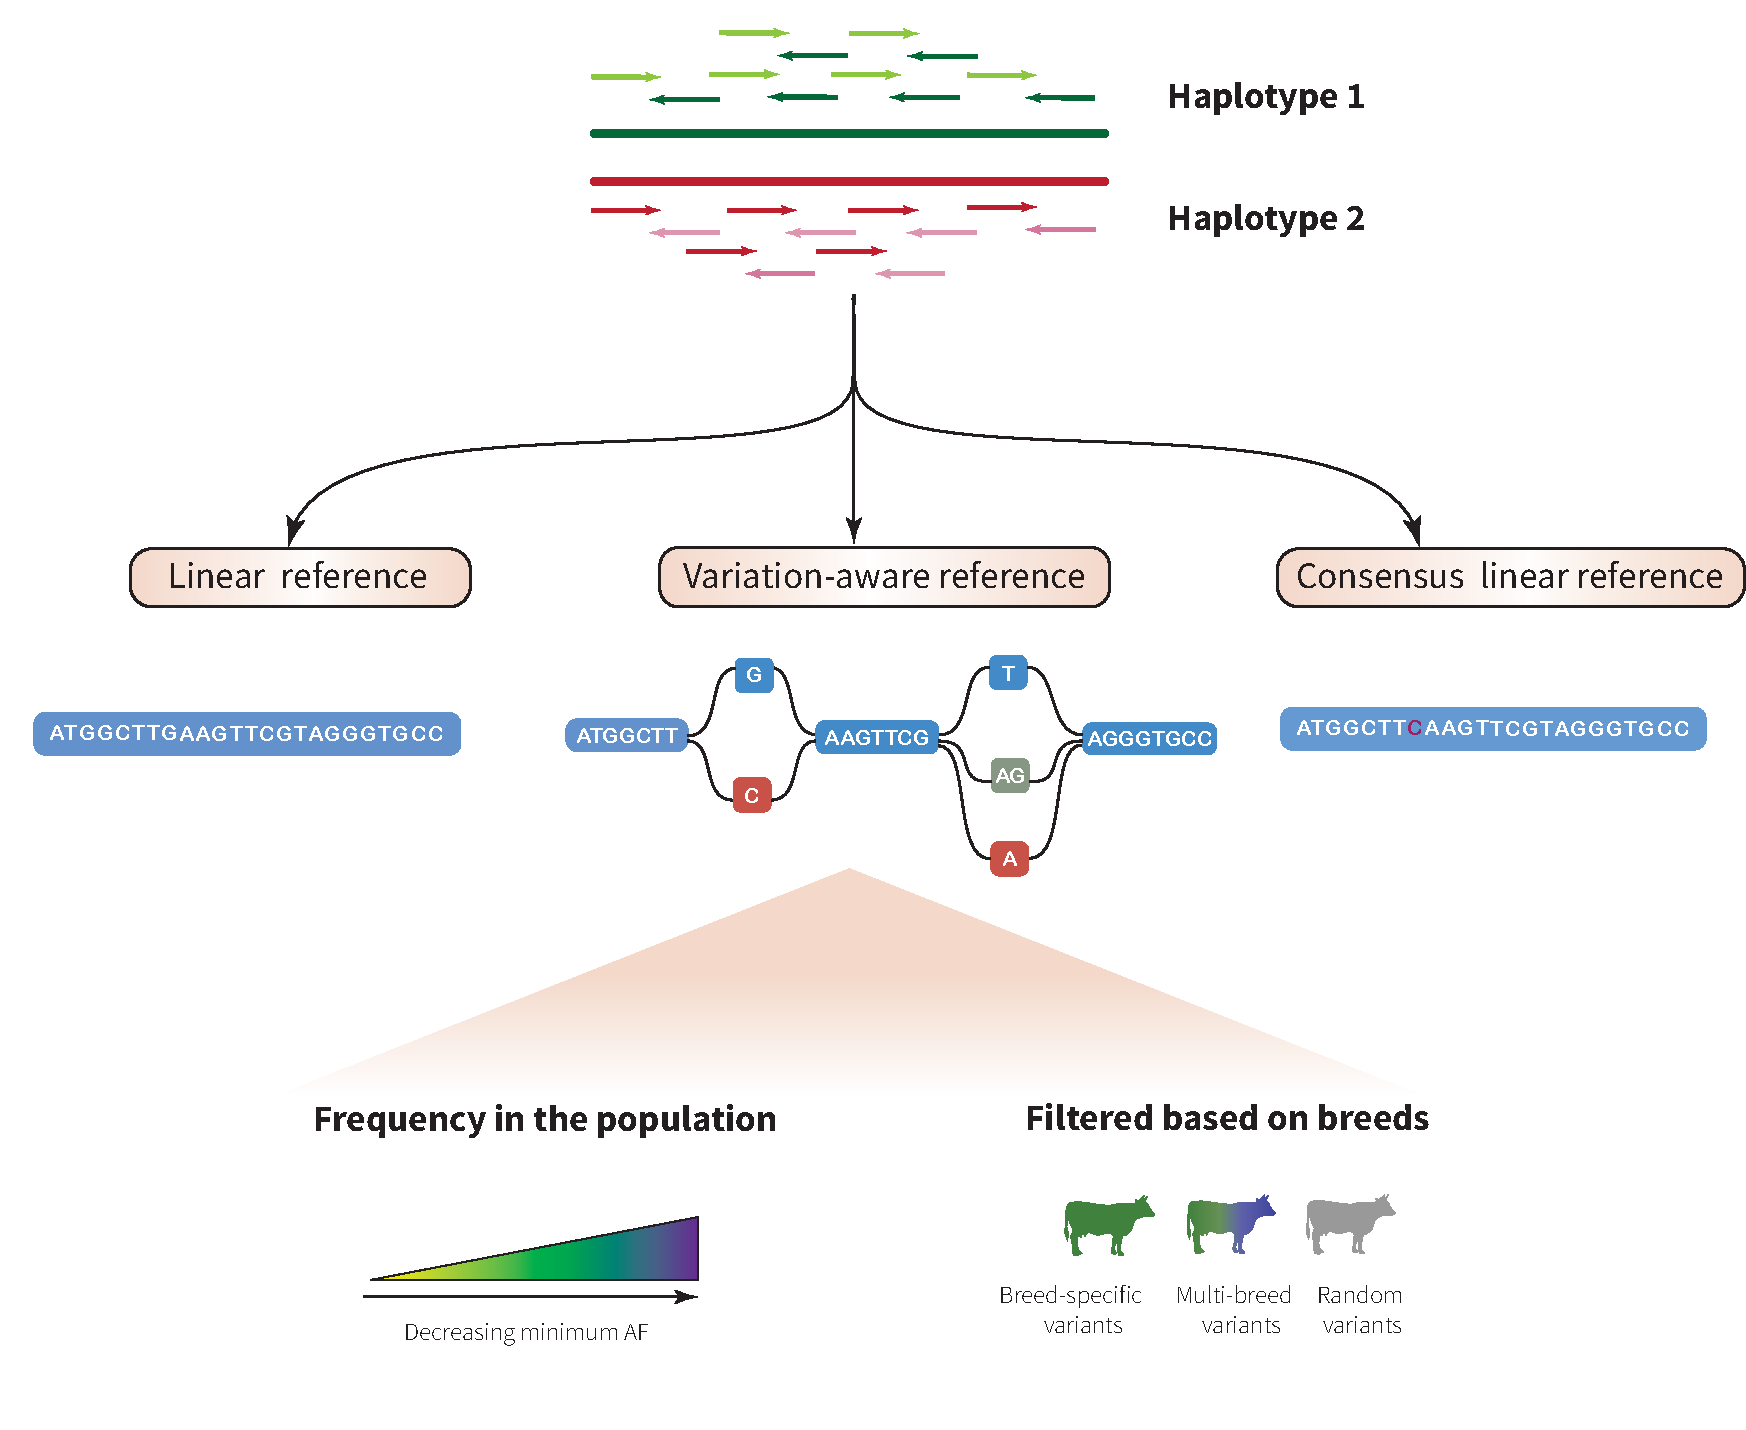
\includegraphics[width=\textwidth]{paper2/main_figure/Fig1.pdf}
    \caption[Schematic overview of the construction of breed-specific augmented genome graphs]{\textbf{Schematic overview of the construction of breed-specific augmented genome graphs.} 
    \small{We used the \emph{vg toolkit} to augment the bovine linear reference sequence (ARS-UCD1.2) with alleles at SNPs and Indels that were discovered in 288 cattle from four breeds. Alleles that were added to the linear reference were prioritized based on their alternate allele frequency (AF). Reads simulated from true haplotypes were aligned to variation-aware, linear and consensus reference sequences to assess read mapping accuracy on cattle chromosome 25. Short-read sequencing data of Brown Swiss cattle were used to investigate sequence variant genotyping accuracy and reference allele bias using a bovine whole-genome graph as a novel reference.}}
    \label{fig31:pipe}
\end{figure}

\section{Results}

\subsection*{Construction of bovine breed-specific augmented genome graphs}

Breed-specific augmented reference graphs were constructed for four genetically distinct dairy (Brown Swiss (BSW), Holstein (HOL)) and dual-purpose (Fleckvieh (FV), Original Braunvieh (OBV)) cattle breeds using the Hereford-based linear reference sequence (ARS-UCD1.2) of chromosome 25 as a backbone (Fig. \ref{fig32:freq}a). Average nucleotide diversity ($\pi$) estimated using 295,801 (HOL), 336,390 (FV), 347,402 (BSW), and 387,855 (OBV) biallelic variants of chromosome 25 ranged from 0.00177 (BSW) to 0.0019 (OBV) for the four breeds (Fig. \ref{fig32:freq}b). To determine the optimal composition of bovine variation-aware references, we augmented the linear reference of chromosome 25 with an increasing number of variants (SNPs and Indels) that were filtered for alternate allele frequency in 82 BSW, 49 FV, 49 HOL, and 108 OBV cattle. In total, we constructed 20 variation-aware graphs for each breed that contained between 2046 (variants had alternate allele frequency $>$ 0.9) and 293,804 (no alternate allele frequency threshold) alleles.

\begin{figure}[!htb]
    \centering
    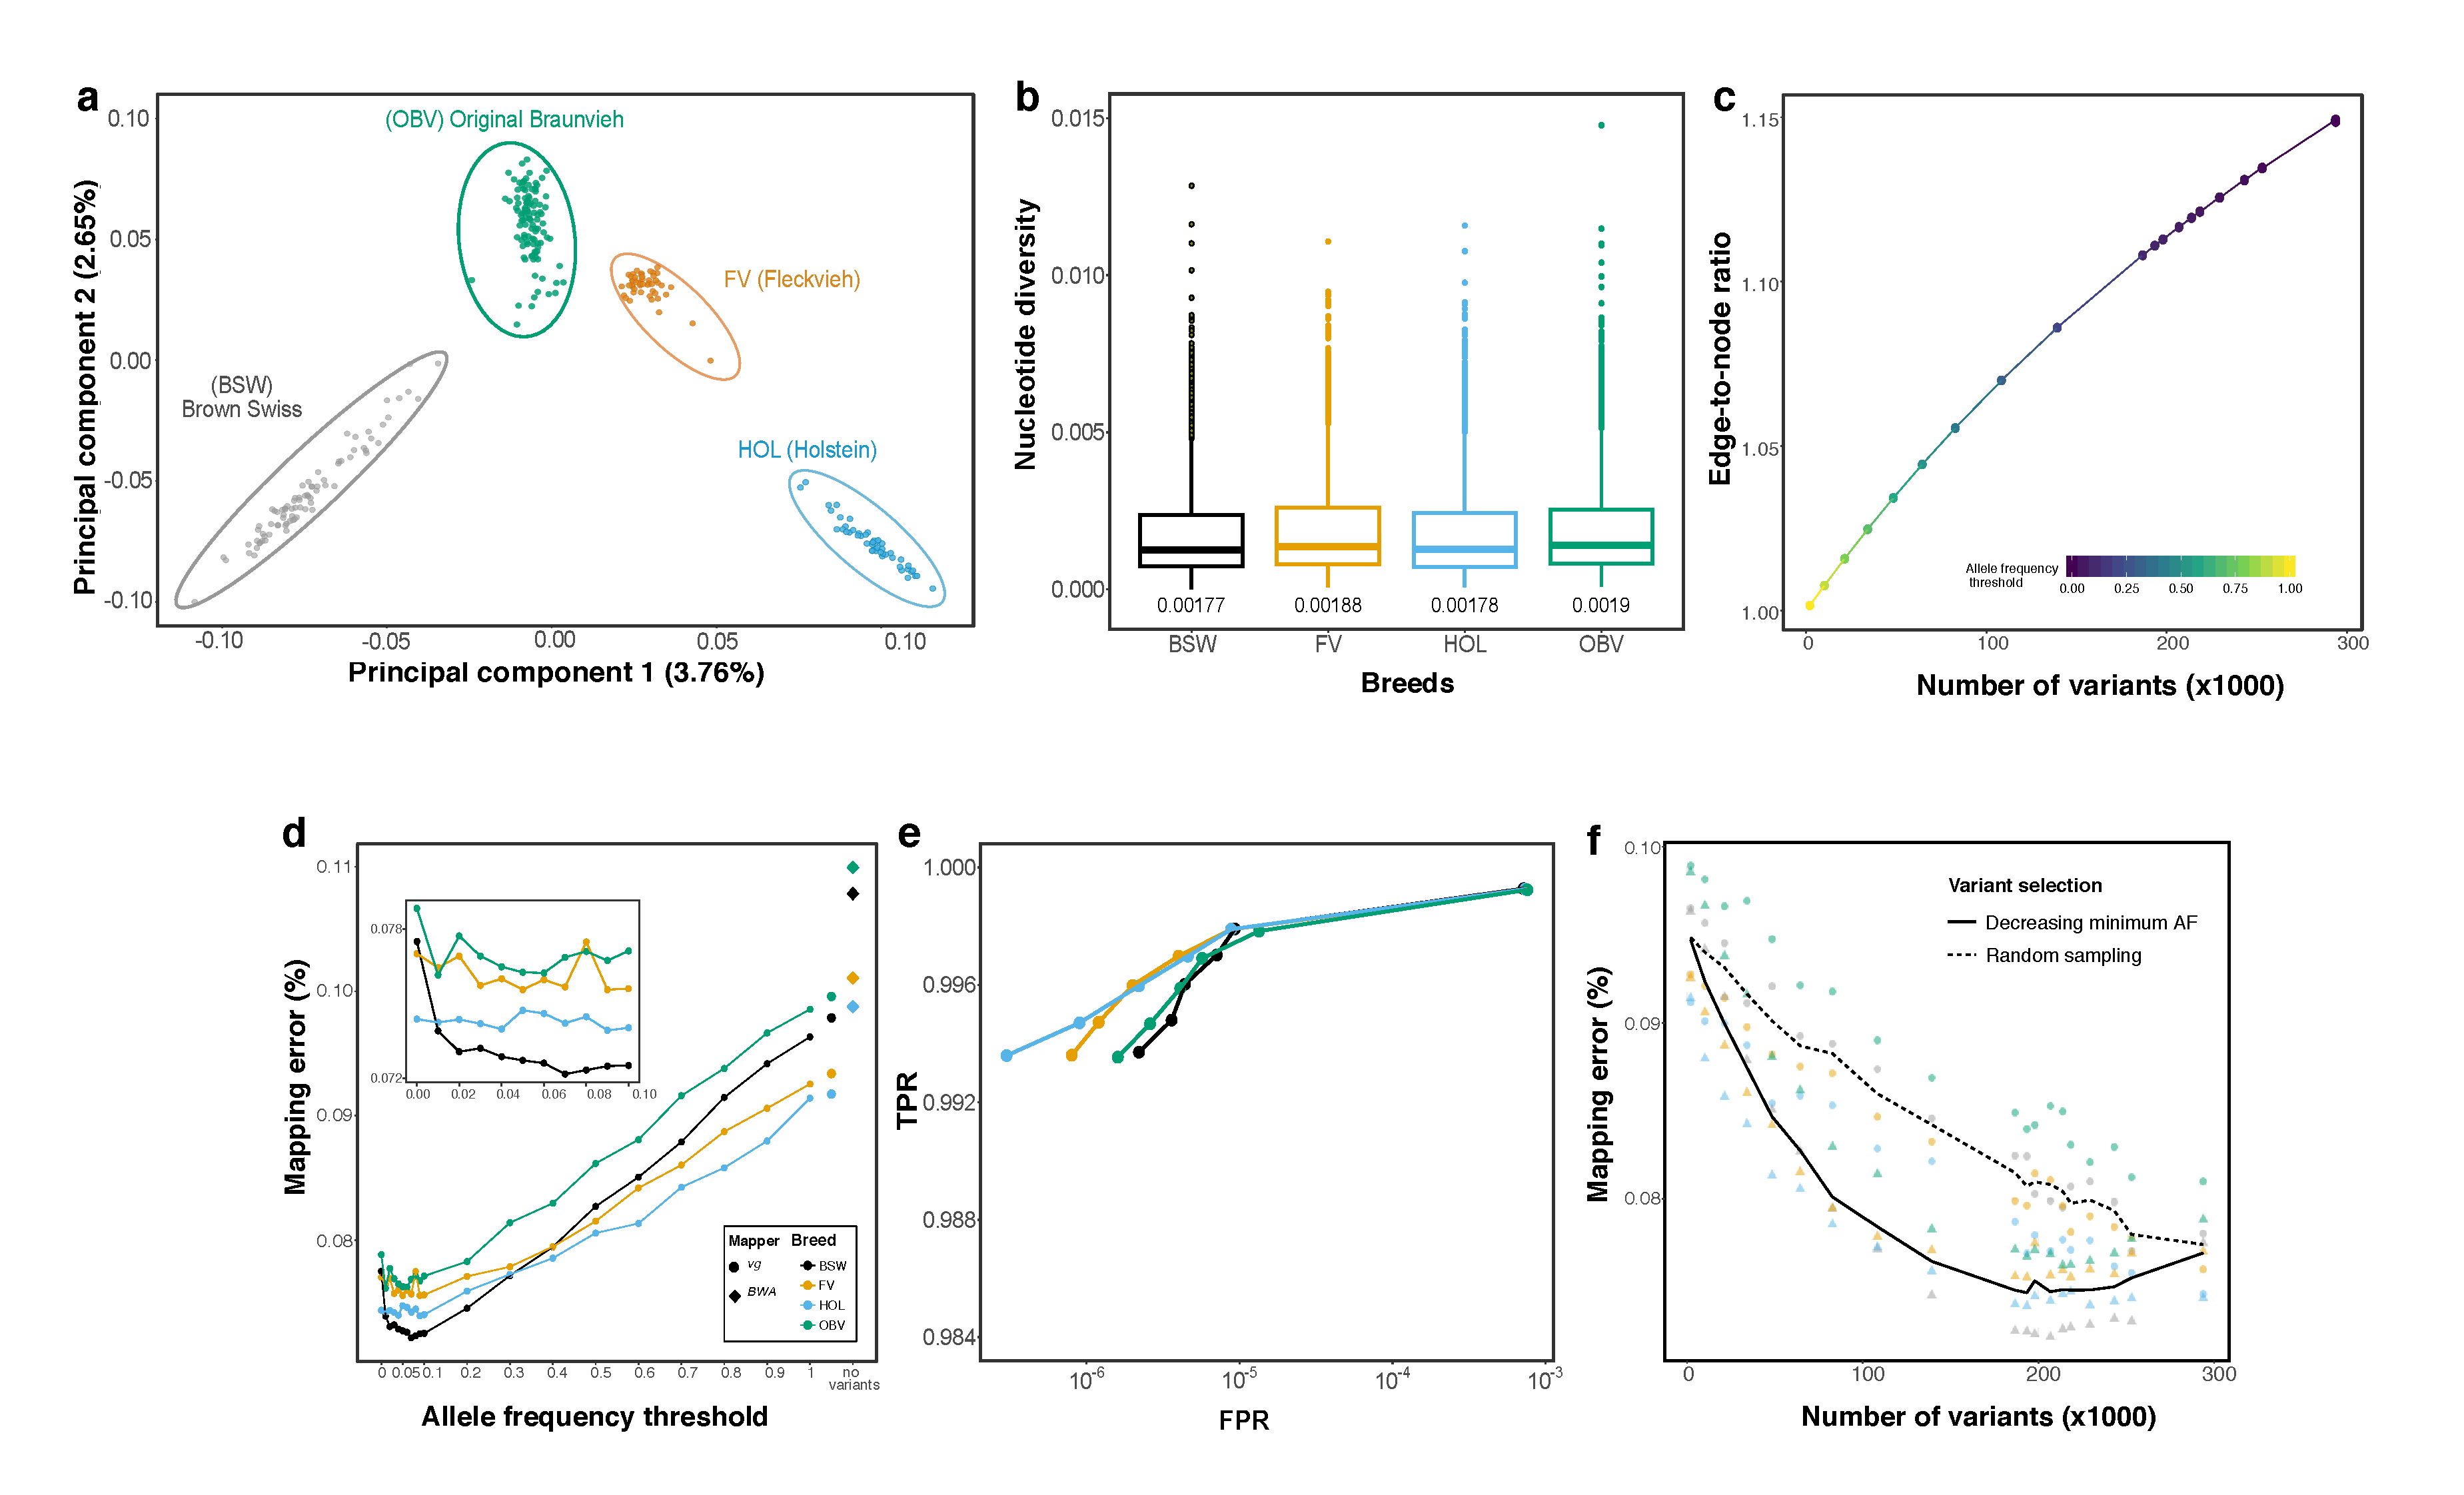
\includegraphics[width=\textwidth]{paper2/main_figure/Fig2.pdf}
    \caption[Accuracy of mapping simulated paired-end reads to genome graphs that contained variants filtered for allele frequency at chromosome 25]{\textbf{Accuracy of mapping simulated paired-end reads to genome graphs that contained variants filtered for allele frequency at chromosome 25.} 
    \small{\textbf{a} The top principal components of a genomic relationship matrix constructed from whole-genome sequence variants reflect the genetic diversity of the four cattle breeds considered. \textbf{b} Nucleotide diversity of the four breeds calculated in non-overlapping 10-kb windows for variants of chromosome 25. The values below each boxplot indicate the nucleotide diversity for the four breeds averaged across all sliding-windows. \textbf{c} Edge-to-node ratio of graphs that contained between 2046 and 293,804 variants filtered for allele frequency. \textbf{d} Proportion of incorrectly mapped reads for four breed-specific augmented genome graphs. Diamonds and large dots represent values from linear mapping using \emph{BWA mem} and \emph{vg}, respectively. The inset represents a larger resolution of the mapping accuracy for alternate allele frequency thresholds less than 0.1. \textbf{e} True-positive (sensitivity) and false-positive mapping rate (specificity) parameterized on mapping quality of the best performing graph from each breed. \textbf{f} Read mapping accuracy for breed-specific augmented graphs that contained variants that were either filtered for alternate allele frequency (triangles) or sampled randomly (circles) from all variants detected within a breed. The dashed and solid line represents the average proportion of mapping errors across four breeds using random sampling and variant prioritization, respectively. Colors indicate values obtained for different breeds. Results for single-end mapping are presented in Fig. \ref{sup_fig:s32}.}}
    \label{fig32:freq}
\end{figure}


The graph-based representation of bovine chromosome 25 (42,350,435 nucleotides) had 1,323,451 nodes and 1,323,450 edges. The number of nodes increased proportionally with the number of variants added to the reference. When we added a maximum number of 293,804 variants to the linear reference sequence of chromosome 25, the variation-aware graph contained 2.02 million nodes. The number of edges increased faster than the number of nodes, ranging from 1.32 (empty) to 2.33 (293,804 variants included) million. Consequently, the edge-to-node ratio increased when variants were added to the graph (Fig. \ref{fig32:freq}c). The number of paths through a graph grows rapidly with the number of variants being added to the graph. The index for the chromosome 25 reference graph contained 84.69 and 118.82 million $k$-mers ($k$ = 256) when 2046 and 293,804 variants, respectively, were added to the graphs (Fig. \ref{sup_fig:s31}).


\subsection*{Variant prioritization based on allele frequency}
We simulated 10 million paired-end reads (2 x 150 bp) corresponding to approximately 35-fold coverage of bovine chromosome 25 from haplotypes of BSW, FV, HOL, and OBV cattle. Using either \emph{BWA mem} or \emph{vg}, we mapped the simulated reads to the respective breed-specific augmented reference graphs and the linear reference sequence. Variants that were only detected in animals used for read simulation were not added to the breed-specific augmented genome graphs. We observed fewer mapping errors using \emph{vg} than \emph{BWA mem} when simulated reads were aligned to a linear reference sequence. This finding was consistent for the four breeds investigated (Fig. \ref{fig32:freq}d). Variation-aware references that contained variants filtered for allele frequency in the respective breed reduced the mapping errors for all breeds. The proportion of reads with mapping errors decreased significantly with the number of variants added to the genome graph (Fig. \ref{fig32:freq}d, Pearson R $=$ 0.94, $P$ $<$ 10$^{-16}$).

Read mapping accuracy increased almost linearly between alternate allele frequency threshold 1 and 0.1, i.e., until 186,680 variants with allele frequency greater than 0.1 were added to the graph (Pearson R $=$ 0.94, $P$ $<$ 10$^{-16}$). Adding additional alleles that had alternate allele frequency between 0.1 and 0.01 to the graphs did not further improve read mapping accuracy over the scenario with an alternate allele frequency threshold of 0.1 ($P$ $=$ 0.13, Fig. \ref{fig32:freq}d inset). Read mapping accuracy declined (particularly in BSW) when the graphs contained rare alleles (alternate allele frequency $<$ 0.01) likely because such alleles are not observed in most animals of a population. Maximum read mapping accuracy was achieved at allele frequency thresholds between 0.2 and 0.01, when the graphs contained between 139,322 and 293,628 variants filtered for allele frequency. The number of erroneously mapped reads was clearly higher for graphs that contained randomly sampled than prioritized variants (Fig. \ref{fig32:freq}f). This finding corroborates that variant prioritization based on alternate allele frequency is important to achieve high mapping accuracy with graph-based reference structures.

We also applied the methods implemented in the FORGe software \citep{pritt2018forge} to prioritize variants for the breed-specific augmented graphs (\ref{sup_not:s31}). It turned out that genome graphs that were constructed with variants selected by the \emph{Pop Cov} strategy, which relies solely on variant frequency information, enabled the highest mapping accuracy improvements over the linear reference. For example, we achieved the highest paired-end read mapping accuracy for the Brown Swiss reference graph (0.0722\% erroneously mapped reads) using the \emph{Pop Cov} method when 208,288 variants were added to the chromosome 25 reference (i.e., the top 60\% of the ranked variants). The prioritized variants correspond to an alternate allele frequency threshold of 0.06. Variant prioritization approaches that also take into account factors other than allele frequency, e.g., the proximity of a variant to an already added variant in the graph or the repetitiveness of the resulting genome graph, did not lead to additional accuracy improvements.

Read mapping accuracy was highly correlated (Pearson R $=$ 0.94, $P$ $<$ 10$^{-16}$) for single- and paired-end reads (Fig. \ref{sup_fig:s32}). However, the accuracy improvement of variation-aware over linear mapping was higher for single- than paired-end reads, possibly because distance and sequence information from paired reads facilitate linear read alignment.

Read mapping accuracy differed significantly among the four breeds analyzed ($P$ $=$ 10$^{-15}$, linear model with allele frequency as covariate) although all breed-specific augmented graphs contained the same number of variants at each allele frequency threshold (Fig. \ref{fig32:freq}d). Linear mapping accuracy also differed among the breeds. We observed the highest error rate for reads aligned to the OBV-specific augmented reference graph. In 500 randomly sampled subsets of 35 sequenced cattle per breed, we discovered more sequence variants on chromosome 25 in OBV (N $=$ 305 $\pm$ 5K) than either FV (N $=$ 291 $\pm$ 3K), BSW (N $=$ 276 $\pm$ 6K) or HOL (N $=$ 259 $\pm$ 2K), reflecting that nucleotide diversity is higher in OBV than the other three breeds, which agrees with a recent study \citep{bhati2020assessing}. Across all alternate allele frequency thresholds considered, read mapping was more accurate for HOL than FV and OBV cattle, possibly because both genetic diversity and effective population size is less in HOL than the other breeds considered \citep{signer2017population}. At allele frequency thresholds between 0.02 and 0.3, read mapping was more accurate for BSW than the other breeds. The proportion of variants with alternate allele frequency larger than 0.02 was lower for BSW(84.1\%) than other breeds (86.3$-$89.2\%). We detected more rare variants (allele frequency less than 0.05) in BSW and OBV than FV and HOL, likely reflecting differences in sample size (Fig. \ref{sup_fig:s33}). An excess of singletons and rare variants in BSW and OBV cattle may have contributed to the decline in mapping accuracy at low alternate allele frequency thresholds (Fig. \ref{fig32:freq}d inset, Table \ref{sup_tab:s32}). Our findings indicate that differences in nucleotide diversity and allele frequency distributions across populations may affect read mapping accuracy to both linear and breed-specific augmented reference structures.

\subsection*{Comparison between bovine and human genome graphs}

We used publicly available whole-genome sequence variant data from phase 3 of the 1000 Genomes Project \citep{10002015global} to construct genome graphs for four genetically distinct human populations (Fig. \ref{fig33:hum}a, GBR (British, European), YRI (Yoruba Nigeria, African), STU (Sri Lankan Tamil, South Asia), and JPT (Japanese, East Asia)). The effective population size is more than 20-fold higher for the human than cattle populations (e.g., $\sim$ 3100 for JPT and $\sim$ 7500 for YRI \citep{tenesa2007recent} vs. $\sim$ 80 for OBV and $\sim$ 160 for FV \citep{pausch2013imputation,hagger2005estimates}). While the average number of sequence variants detected per sample was lower for the human than cattle populations (4,248,082 vs. 6,973,036), the proportion of singletons is higher in the human than cattle samples (23.00\% in human vs. 14.01\% in cattle) Table (\ref{sup_tab:s31}). The proportion of sequence variants that had minor allele frequency less than 0.05 was between 44.88 and 55.45\% in the four human and between 23.65 and 38.70\% in the four cattle populations (Fig. \ref{sup_fig:s34}). Nucleotide diversity ranged from 0.00098 (JPT) to 0.00141 (YRI) (Fig. \ref{fig33:hum}b).

\begin{figure}[!htb]
    \centering
    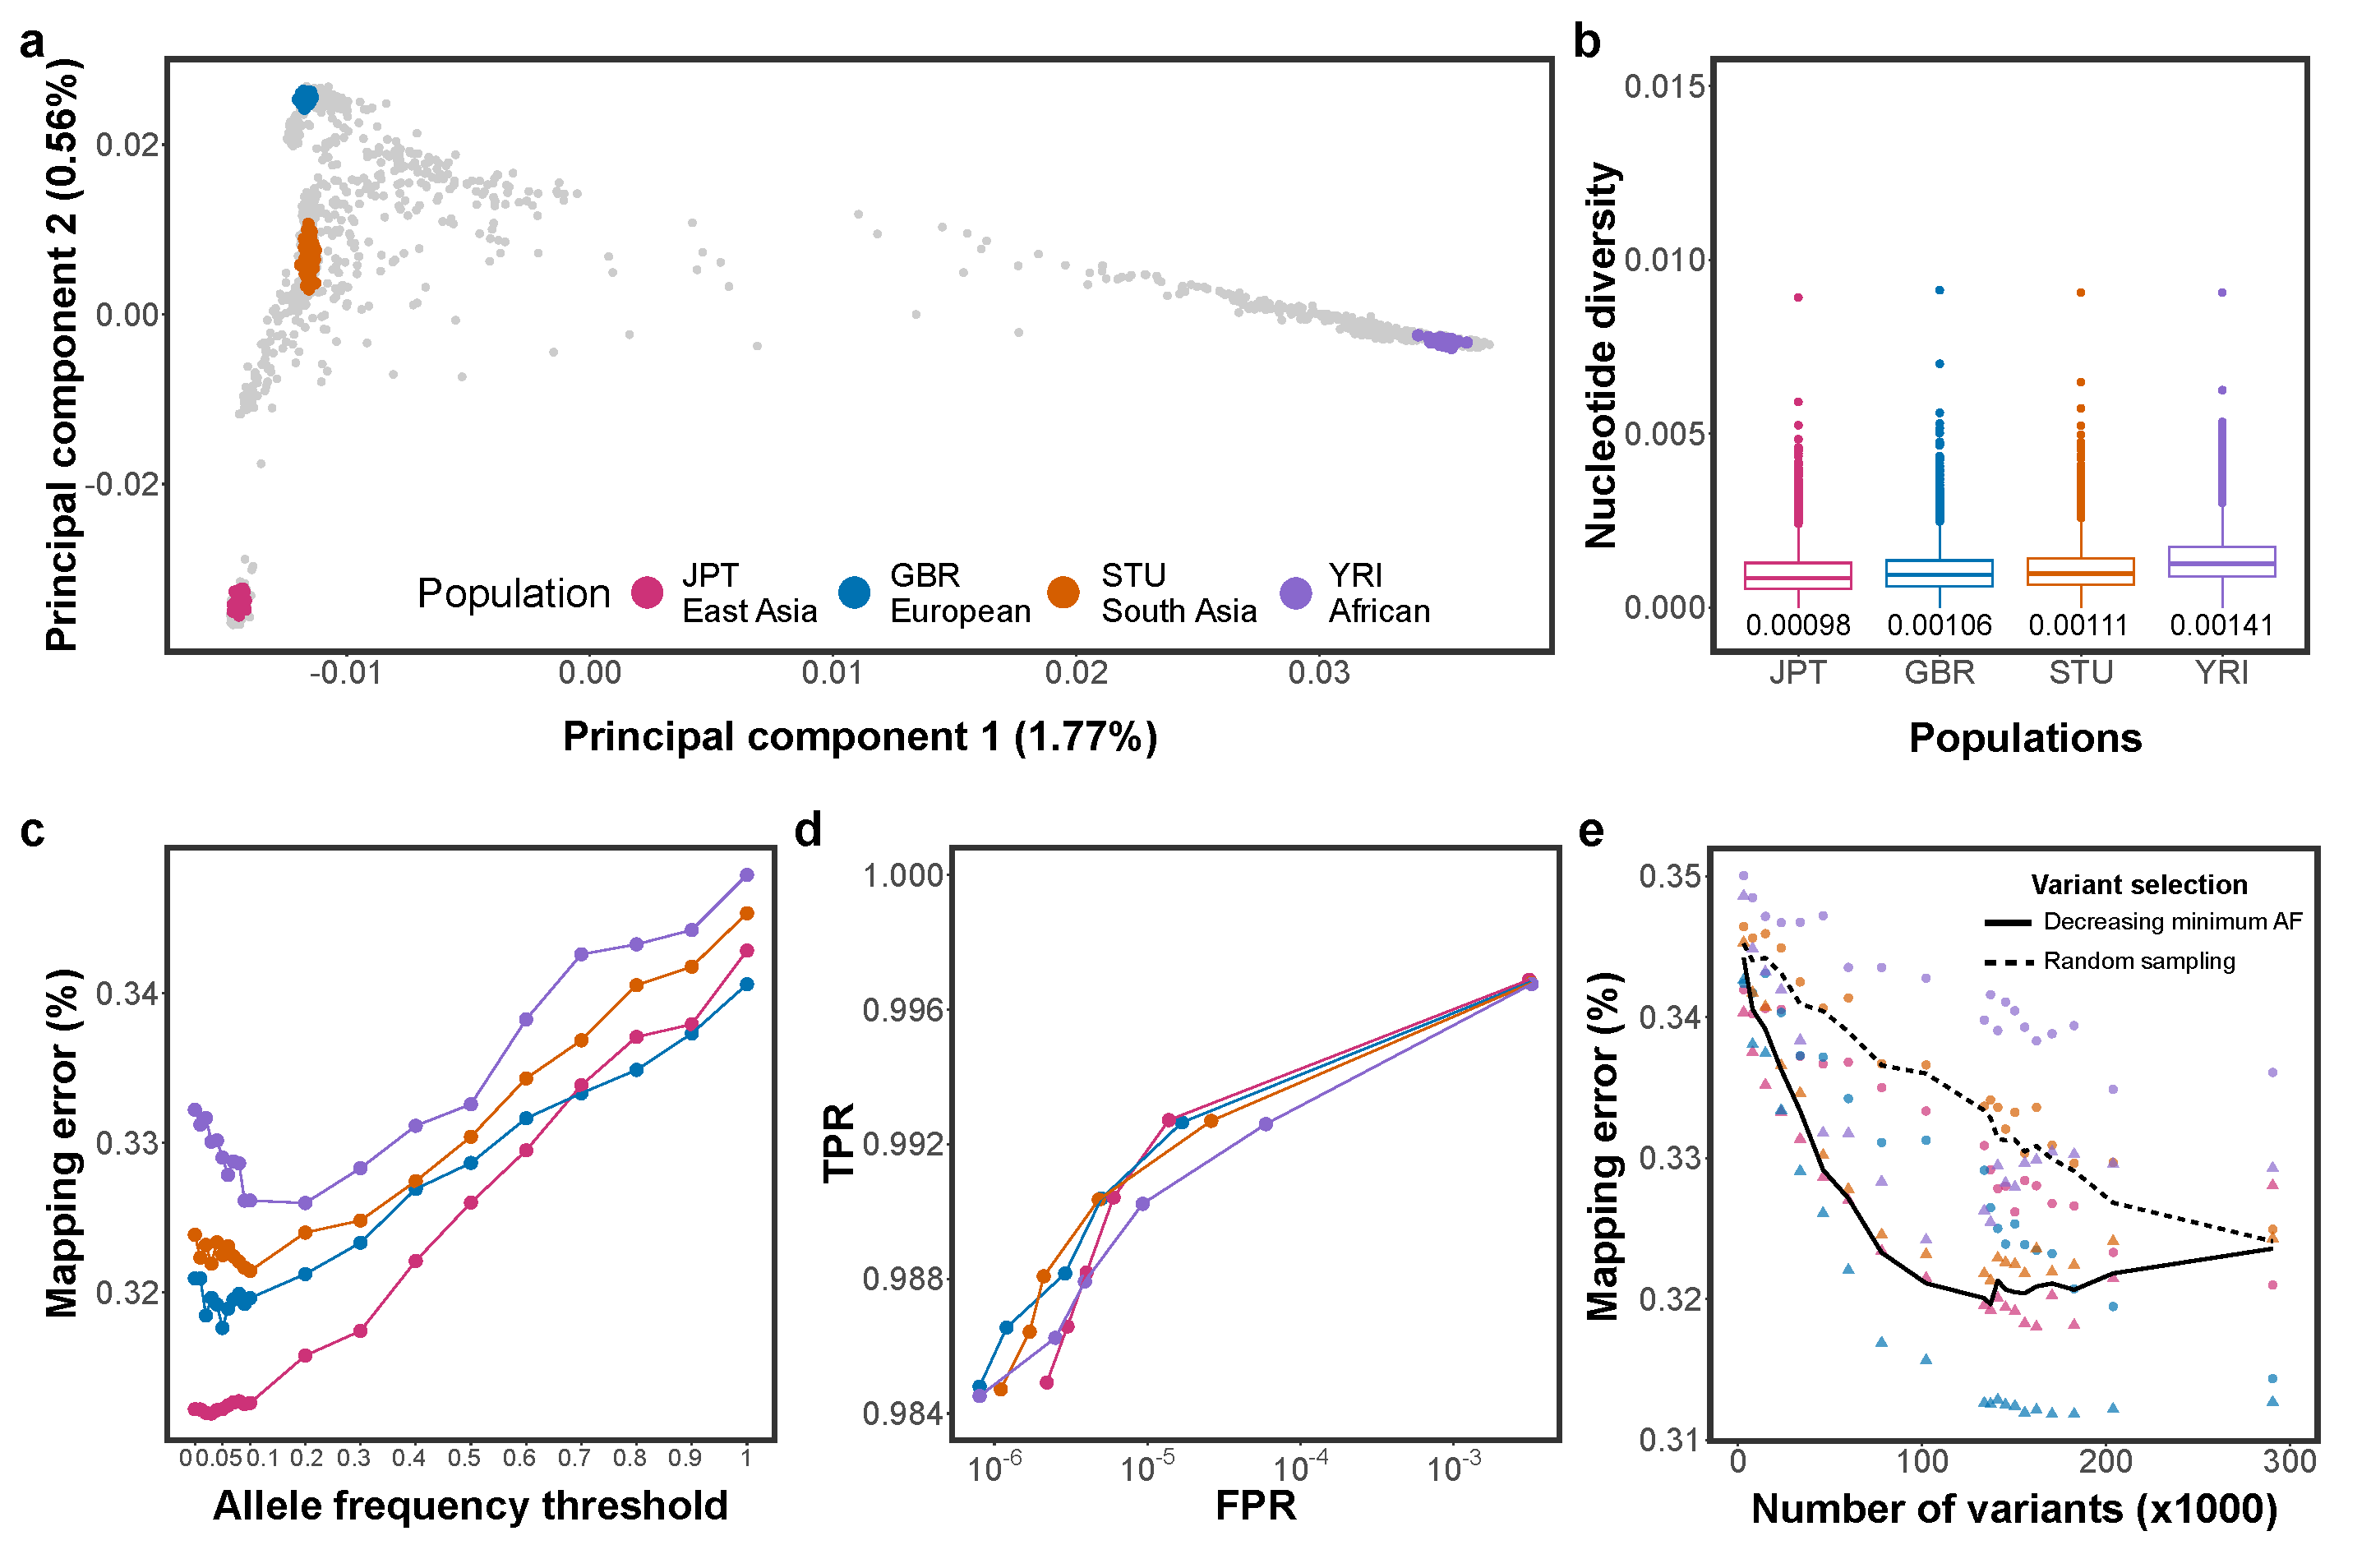
\includegraphics[width=\textwidth]{paper2/main_figure/Fig3.pdf}
    \caption[Accuracy of mapping simulated paired-end reads to human population-specific augmented genome graphs]{\textbf{Accuracy of mapping simulated paired-end reads to human population-specific augmented genome graphs.}
    \small{\textbf{a} The top principal components of a genomic relationship matrix constructed from autosomal variants detected in 2504 individuals that were included in phase 3 of the 1000 Genomes Project. The colored points indicate 405 samples from the GBR (European), YRI (African), STU (South Asia), and JPT (East Asia) populations. \textbf{b} Nucleotide diversity of the four populations calculated in non$-$overlapping 10 kb windows for variants of chromosome 19. The values below each boxplot indicate the nucleotide diversity for the four populations averaged across all sliding-windows. \textbf{c} Proportion of incorrectly mapped reads for four population-specific augmented genome graphs. \textbf{d} 
    True\-positive (sensitivity) and false\-positive mapping rate (specificity) parameterized on mapping quality of the best performing graph from each population. \textbf{e} Read mapping accuracy for population-specific augmented graphs that contained variants that were either filtered for alternate allele frequency (triangles) or sampled randomly (circles) from all variants detected within a population. The dashed and solid line represents the average proportion of mapping errors across four populations using variant prioritization and random sampling, respectively. Results for single-end mapping are presented in Fig \ref{sup_fig:s36}}}
    \label{fig33:hum}
\end{figure}

We considered the linear reference sequence of human chromosome 19 (g1k\_v37 ref) as a backbone for the human genome graphs because its length (59,128,893 bp) and the number of variants detected per sample was similar to the values for bovine chromosome 25. Genetic diversity and allele frequency distributions were similar using either chromosome 19 or whole-genome variants indicating that the results obtained using chromosome 19 are representative for the human genome (Figs. \ref{sup_fig:s34}, \ref{sup_fig:s35}, Table \ref{sup_tab:s32}). To construct population-specific augmented graphs, we used phased genotypes at 291,303, 306,304, 355,107, and 521,021 variants of chromosome 19 that were available for 104 JPT, 91 GBR, 102 STU, and 108 YRI individuals. Once the variants that were only detected in individuals used for simulating reads were removed from the graphs, the population-specific augmented graphs for the GBR, YRI, STU, and JPT populations contained between 3153 
(alternate allele frequency $>$ 0.9) and 290,593 (no alternate allele frequency threshold) variants. We subsequently simulated 10 million reads from haplotypes of one individual per population and mapped the reads to the respective population-specific augmented genome graphs.

As observed for the bovine breed-specific augmented genome graphs, read mapping accuracy increased almost linearly between alternate allele frequency threshold 1 (no variants included) and 0.1 (133,891 variants added to the graph) (Fig. \ref{fig33:hum}c). Adding low-frequency variants (alternate allele frequency between 0.01 and 0.1) did not further improve the mapping accuracy. Mapping accuracy decreased for all graphs when we added very rare variants and singletons to the graphs. This pattern was most apparent for YRI which had the highest proportion of rare variants and nucleotide diversity among the four populations considered. Read mapping accuracy differed among the four populations analyzed. We observed the lowest number of mis\-mapped reads when reads simulated from a JPT individual were aligned to a JPT-specific augmented genome graph. The highest number of mis-mapped reads was observed when reads simulated from a YRI individual were aligned to a YRI-specific augmented genome graph. Mapping accuracy was higher for GBR than STU. These findings indicate that the mapping accuracy is negatively correlated with nucleotide diversity. Mapping accuracy improvements over the linear reference sequence were less when randomly sampled variants were added to the graphs (Fig. \ref{fig33:hum}e).

While the overall pattern of the mapping accuracy improvements over the linear reference was similar for human and bovine genome graphs across all allele frequency thresholds considered, the proportion of mis-mapped paired-end reads was approximately four-fold higher in the human than bovine alignments (two-fold for single-end reads; \ref{sup_fig:s36}). This finding was also apparent when the population-specific augmented graphs were parameterized on mapping quality to obtain sensitivity and specificity (Fig. \ref{fig32:freq}e and Fig. \ref{fig33:hum}d).

\subsection*{Mapping to breed-specific augmented genome graphs}

Next, we compared read mapping accuracy between bovine breed-specific augmented and pan-genome graphs (i.e., graphs that contained variants filtered for allele frequency across multiple populations) using reads simulated from phased variants of bovine chromosome 25. We constructed four breed-specific augmented genome graphs that contained variants that had alternate allele frequency $>$ 0.03 in either the BSW, FV, HOL, or OBV breeds. HOL had the lowest number of variants (N $=$ 243,145) with alternate allele frequency $>$ 0.03, reflecting that sample size was lower in HOL than the other breeds. To ensure that the density of information was comparable across all breed-specific augmented graphs, we randomly sampled 243,145 variants with alternate allele frequency $>$ 0.03 from the BSW, FV, and OBV populations and added them to the respective graphs. The pan-genome graph contained variants that had alternate allele frequency $>$ 0.03 in 288 individuals from the four populations. The random graph contained 243,145 randomly sampled variants for which haplotype phase and the allele frequency in the BSW, FV, HOL, or OBV breeds was unknown (see the \nameref{chap3:meth}  section). To investigate read mapping accuracy, we simulated 10 million sequencing reads (150 bp) from BSW haplotypes and mapped them to the variation-aware and linear reference sequences. Variants that were only detected in the BSW animal used for simulating reads were excluded from the graphs. However, in order to determine an upper bound for graph-based read mapping accuracy, we also constructed a “personalized” genome graph, i.e., a graph that contains only haplotypes of the animal used for simulating the reads. We repeated the selection of variants, construction of variation-aware graphs and subsequent read mapping ten times.

The average length, number of nodes, number of edges, and edge-to-node ratio of the variation-aware graphs were 42.60 Mb, 1,907,248, 2,155,799, and 1.13, respectively. Most variants of the random graph (87.81\%) were not detected at alternate allele frequency $>$ 0.03 in BSW, FV, OBV, and HOL indicating that they were either very rare or did not segregate in the four breeds considered in our study. Of 243,145 variants, an intersection of 48.13\% had alternate allele frequency greater than 0.03 in the four breeds considered (Fig. \ref{fig34:breed}a). The average number of variants that were specific to the breed-specific augmented graphs ranged from 8010 in BSW to 20,392 in FV.

\begin{figure}[!htb]
    \centering
    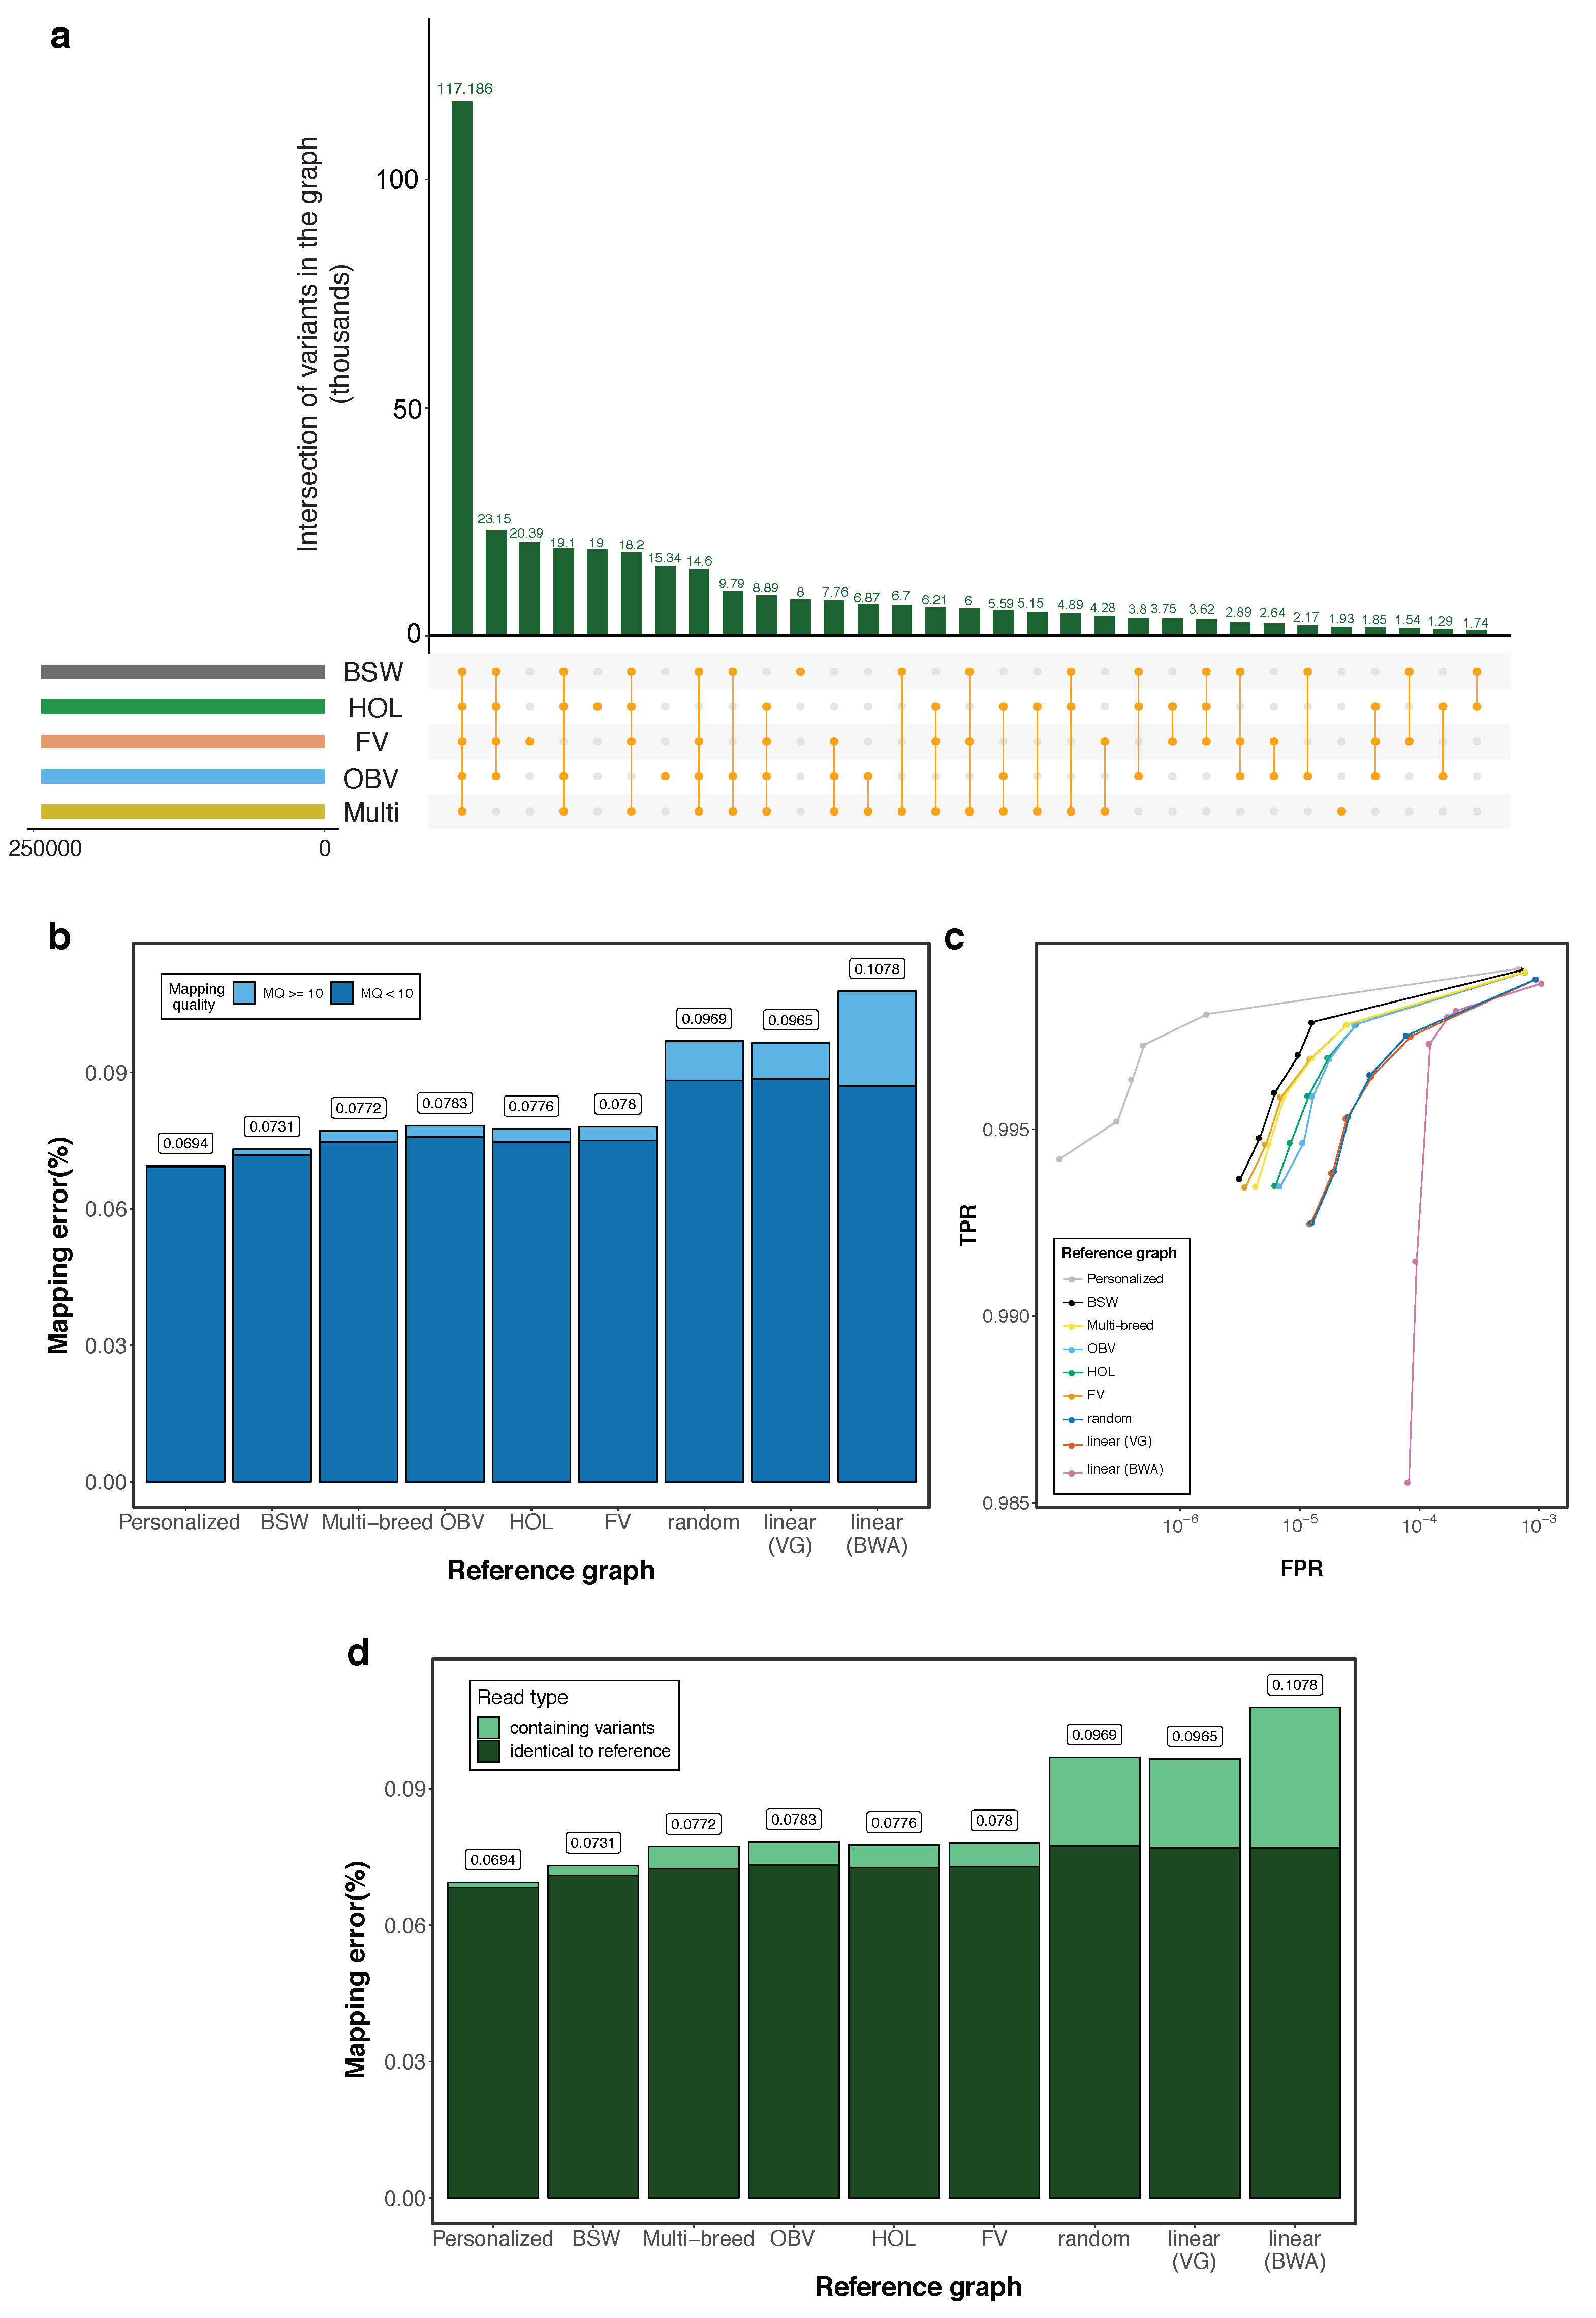
\includegraphics[width=\textwidth]{paper2/main_figure/Fig4.pdf}
\end{figure}

\begin{figure}[!htb]
    \centering
    \caption[The accuracy of mapping simulated BSW paired-end reads to variation-aware and linear reference structures]{\textbf{The accuracy of mapping simulated BSW paired-end reads to variation-aware and linear reference structures.}\small{ \textbf{a} We added 243,145 chromosome 25 variants to the Hereford-based reference sequence that were filtered for alternate allele frequency $>$ 0.03 in either the BSW, FV, HOL, or OBV populations. The pan-genome graph (Multi) contained 243,145 variants that had alternate allele frequency threshold $>$ 0.03 across 288 cattle from the four breeds considered. The bars indicate the overlap of variants (averaged across ten replications) that were added to different graphs. \textbf{b} Proportion of simulated BSW reads that mapped erroneously against personalized graphs, breed-specific augmented graphs, pan-genome graphs (Multi-breed), random graphs, or linear reference sequences. We used \emph{vg} and \emph{BWA mem} for linear mapping. Dark and light blue colors represent the proportion of incorrectly mapped reads that had phred-scaled mapping quality (MQ) $<$ 10 and MQ $>$ 10, respectively. \textbf{c} True-positive (sensitivity) and false-positive mapping rate (specificity) parameterized on mapping quality. \textbf{d} Proportion of BSW reads that mapped incorrectly against breed-specific augmented graphs, pan-genome graphs (Multi-breed), random graphs, or linear reference sequences. Dark and light green colors represent the proportion of incorrectly mapped reads that matched corresponding reference nucleotides and contained non-reference alleles, respectively. Results for single-end mapping are presented in Fig. \ref{sup_fig:s37}}}
    \label{fig34:breed}
\end{figure}


Personalized genome graphs, i.e., graphs that are tailored to a specific individual, enable the largest read mapping accuracy improvements over linear references. The proportion of mis-mapped reads was 0.0694\% when a personalized BSW graph was used as a reference. Apart from the personalized graph, the highest mapping accuracy, sensitivity, and specificity was achieved when the simulated BSW reads were aligned to a BSW-specific augmented graph (Fig. \ref{fig34:breed}b–d). The proportion of erroneously mapped paired-end reads was 0.073\% for the BSW-specific augmented graph. Sensitivity and specificity were slightly lower and the number of reads with mapping errors was slightly higher when the same reads were aligned to a pan-genome graph. The read mapping accuracy differed only slightly between the breed-specific augmented and pan-genome graph because the overlap of variants that were included in both variation-aware references was high (Fig. \ref{sup_fig:s38}). The number of mapping errors was higher (adjusted \emph{P} $<$ $^{−16}$, \emph{pairwise t test}, \ref{sup_fig:s39}) when BSW reads were aligned to genome graphs that contained variants filtered for allele frequency in either the FV, HOL, or OBV populations.

We also simulated reads from haplotypes of FV, HOL, and OBV cattle. Similar to our findings using reads simulated from BSW cattle, mapping was more accurate to breed-specific than either pan-genome graphs or graphs that were augmented with variants filtered for allele frequency in other breeds (Fig. \ref{sup_fig:s310}).

Mapping reads to a linear reference sequence using \emph{BWA mem} with default parameter settings was the least sensitive and least specific mapping approach tested. Linear mapping using \emph{vg} was also less accurate than variation-aware mapping. This finding indicates that accuracy improvements of variation-aware over linear mapping are attributable to differences in the reference structure rather than mapping algorithms. All graphs that contained pre-selected variants that had alternate allele frequency greater than 0.03 enabled significantly ($P$ $=$ 10$^{−16}$, \emph{two-sided t test}) higher mapping accuracy than linear references. This was also true when reads were mapped to graphs that contained variants that were filtered for allele frequency in a different breed, likely because many common variants segregated across the four breeds considered (Fig. \ref{fig34:breed}a).

Recently, \citet{grytten2020assessing} showed that an adjusted linear alignment approach that relies on a combination of \emph{BWA mem} and \emph{Minimap2} \citep{li2018minimap2} may improve linear mapping accuracy because the default setting of \emph{BWA mem} might miss sub-optimal alignments and overestimate mapping quality for multi-mapping reads \citep{grytten2020assessing,li2013aligning}. We found that this approach enables to reduce the proportion of mis-mapped from 0.1078 to 0.0983 in cattle (\ref{sup_not:s32}). Improved mapping accuracy from the combination of \emph{BWA mem} and \emph{Minimap2} primarily results from less incorrectly mapped reads that had mapping quality $>$ 10, indicating a better mapping quality assignment. The mapping accuracy from the adjusted linear alignment approach is similar to the linear mapping accuracy obtained using \emph{vg} but considerably lower than using breed-specific augmented graphs (\ref{sup_not:s32}). The number of paired-end reads with mapping errors is 26\% higher using the adjusted linear alignment approach than breed-specific augmented reference graphs.

Reference graphs that contained random variants, i.e., variants that were neither phased, nor filtered for allele frequency in the breeds of interest, did not improve mapping accuracy, sensitivity and specificity over linear references (adjusted \emph{P} $=$ 0.74 and 0.35 for single- and paired-end, \emph{pairwise t test}, Fig. \ref{sup_fig:s39}).

Compared to linear mapping using BWA mem with default parameter settings, the number of mapping errors decreased by 39 and 31\% for single- and paired-end reads, respectively, using a breed-specific augmented reference graph. Extrapolated to whole-genome sequencing data required for a 35-fold genome coverage, the use of breed-specific augmented reference graphs could reduce the number of incorrectly mapped single- and paired-end reads by 1,300,000 and 220,000, respectively.

Using the BSW-specific augmented graph as a reference, only 1.76\% of the incorrectly mapped reads had mapping quality (MQ) greater than 10. The MQ of the vast majority (98.24\%) of incorrectly mapped reads was less than 10, i.e., they would not qualify for sequence variant discovery and genotyping using \emph{GATK} with default parameter settings. The proportion of incorrectly mapped reads with MQ $>$ 10 was twice as high using either the pan-genome or an across-breed augmented reference graph (3.21–3.85\%). The proportion of incorrectly mapped reads with MQ $>$ 10 was higher using either the random graph (8.92\%) or linear reference sequence (\emph{vg}: 8.19\%, \emph{BWA mem}: 19.3\%).

Of 10 million simulated reads, 19.16\% contained at least one nucleotide that differed from corresponding Hereford-based reference alleles. Using \emph{BWA mem}, 47.44\% and 28.72\% of the erroneously mapped single- (SE) and paired-end (PE) reads, respectively, contained alleles that differed from corresponding reference nucleotides indicating that incorrectly mapped reads were enriched for reads that contained non-reference alleles (Fig. \ref{fig34:breed}d, Figs. \ref{sup_fig:s37}, \ref{sup_fig:s311}). The proportion of erroneously mapped reads that contained non-reference alleles was similar for reads that were aligned to either random (47.62\% and 20.13\%) or empty graphs (48.20\% and 20.35\%) using \emph{vg}. However, the proportion of incorrectly mapped reads that contained non-reference alleles was clearly lower for the breed-specific augmented (SE: 1.37\%, PE: 3.08\%) and pan-genome graphs (SE: 2.12\%, PE: 6.14\%). The proportion of incorrectly mapped reads that matched corresponding reference nucleotides was almost identical across all mapping scenarios tested (Figs. \ref{fig34:breed}d, \ref{sup_fig:s37}, \ref{sup_fig:s311}).

Using data from the Ensembl bovine gene annotation (version 99) and RepeatMasker, we determined if the simulated reads originate from either genic regions, interspersed duplications, or low-complexity and simple repetitive regions Fig (\ref{sup_fig:s312}). Regardless of the reference structure used, the mapping accuracy was low for reads originating from repetitive regions. Mapping accuracy was higher for reads originating from either genic or exonic regions. Graph-based references enabled more accurate mapping of reads originating from either genic regions or interspersed duplications (including SINEs, LINEs, LTR, and transposable elements) than linear reference sequences. However, graph-based references did not improve the mapping accuracy over linear references for reads that originate from low-complexity or simple repetitive regions.

We further augmented the BSW-specific genome graph with 157 insertion and deletion polymorphisms of bovine chromosome 25 that were detected from short paired-end reads (2 $×$ 150 bp) of 82 BSW animals using \emph{Delly}. Adding these variants to the graph either alone or in addition to 243,145 variants that were detected using \emph{GATK} did not improve the mapping accuracy over the corresponding scenarios that did not include these variants (\ref{sup_not:s33}).

\subsection*{Linear mapping accuracy using a consensus reference sequence}

Previous studies reported that linear mapping may be more accurate using population-specific than universal linear reference sequences \citep{ballouz2019time,shukla2019hg19kindel,dewey2011phased}. In order to construct bovine linear consensus reference sequences, we replaced the alleles of the chromosome 25 ARS-UCD1.2 reference sequence with corresponding major alleles at 67,142 and 73,011 variants that were detected in 82 BSW and 288 cattle from four breeds, respectively. Subsequently, we aligned 10 million simulated BSW reads to the linear adjusted sequences using either \emph{vg} or \emph{BWA mem}. Read mapping was more accurate to the consensus than original linear reference sequence (Figs. \ref{fig35:consen}, \ref{sup_fig:s313}). The accuracy of mapping was higher when reference nucleotides were replaced by corresponding major alleles that were detected in the target than multi-breed population. However, the mapping of reads was less accurate, sensitive, and specific using either of the consensus linear reference sequences than the breed-specific augmented graphs (Fig. \ref{fig35:consen}b).

\begin{figure}[!htb]
    \centering
    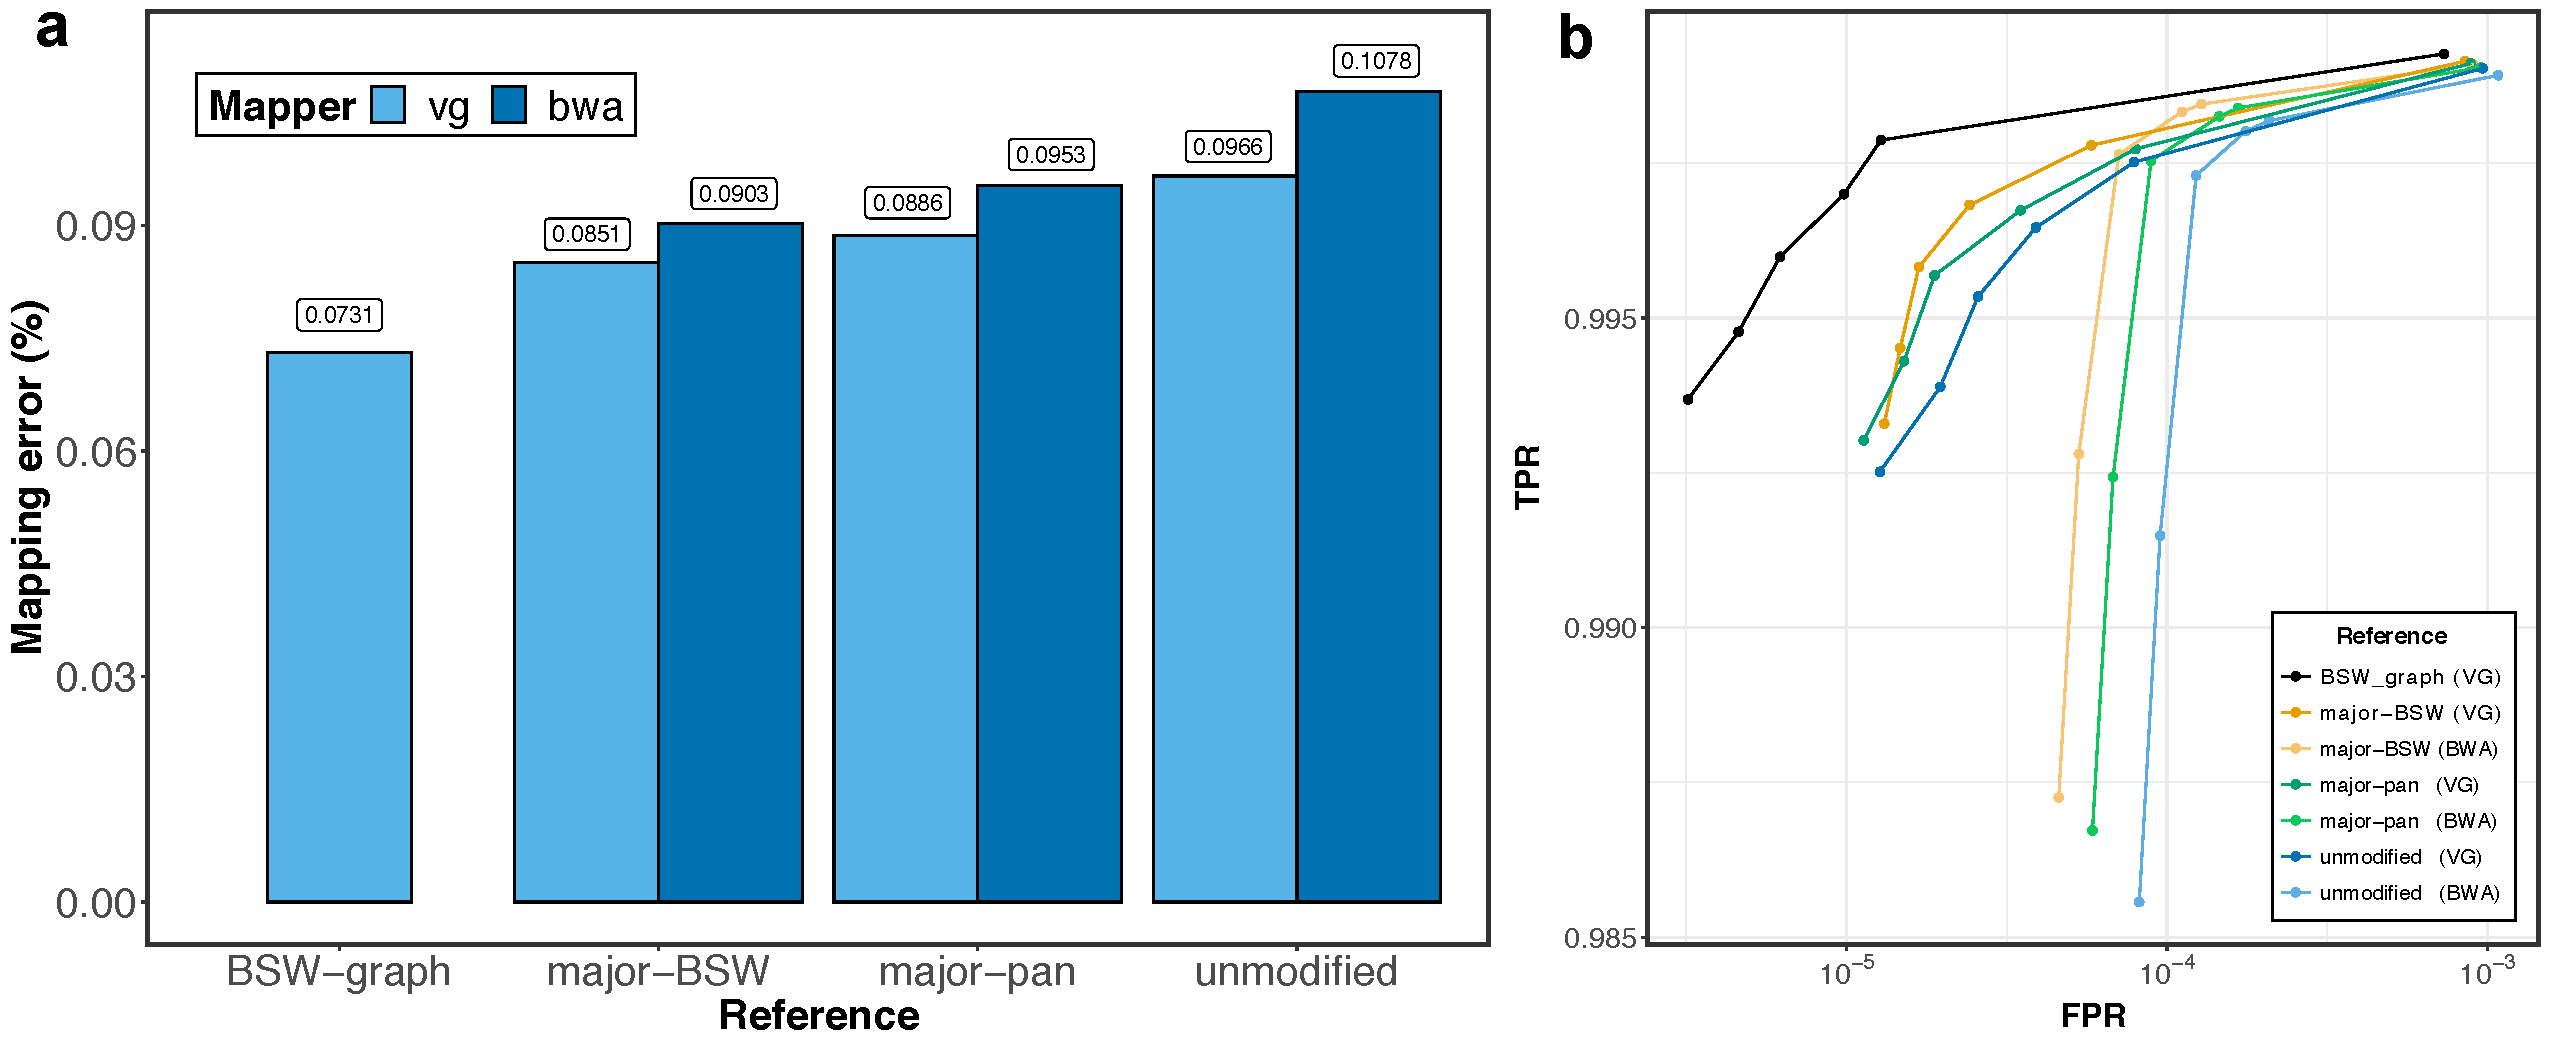
\includegraphics[width=\textwidth]{paper2/main_figure/Fig5.pdf}
    \caption[Paired-end read mapping accuracy using breed-specific augmented genome graphs and consensus linear reference sequences]{\textbf{Paired-end read mapping accuracy using breed-specific augmented genome graphs and consensus linear reference sequences.} 
    \small{\textbf{a} Dark and light blue represent the proportion of reads that mapped incorrectly using \emph{BWA mem} and \emph{vg}, respectively, to the BSW-specific augmented reference graph (BSW-graph), the BSW-specific (major-BSW) and the multi-breed linear consensus sequence (major-pan) and the bovine linear reference sequence (unmodified). \textbf{b} True-positive (sensitivity) and false-positive mapping rate (specificity) parameterized based on the mapping quality. The results of an analysis where reference nucleotides were only replaced at SNPs is available in Fig. \ref{sup_fig:s313}}}
    \label{fig35:consen}
\end{figure}

\subsection*{Read mapping and variant genotyping using whole genome graphs}
In order to develop a breed-specific augmented reference structure for whole-genome applications, we constructed a BSW-specific augmented whole-genome variation-aware reference graph using 14,163,824 autosomal biallelic variants (12,765,895 SNPs and 1,397,929 Indels) that had alternate allele frequency greater than 0.03 in 82 BSW cattle. The resulting graph contained 111,511,367 nodes and 126,058,052 edges (an edge-to-node ratio of 1.13) and 6.32 x 10$^9$ 256-mer paths. We also constructed a linear (empty) whole-genome graph that did not contain allelic variation. Subsequently, we mapped paired-end (2 × 150 bp) sequencing reads of 10 BSW cattle that had been sequenced at between 6- and 40-fold coverage (Table \ref{sup_tab:s34}) to the variation-aware and linear reference sequence using either \emph{vg map} or \emph{BWA mem}. The 10 BSW cattle used for sequence read mapping were different to the 82 animals used for variant discovery, graph construction, and haplotype indexing.

62.19, 51.35 and 49.16\% of the reads aligned perfectly (i.e., reads that aligned with full length (no clipping) and without any mismatches or Indels) to the BSW-specific augmented graph, the empty graph, and the linear reference sequence, respectively (Fig. \ref{fig36:whole}a). We observed slightly less uniquely mapped reads using either the whole-genome (82.46\%) or empty graph (82.18\%) than the linear reference sequence (83.18\%) indicating that variation-aware references can increase mapping ambiguity due to providing alternative paths for read alignment.

\begin{figure}[!htb]
    \centering
    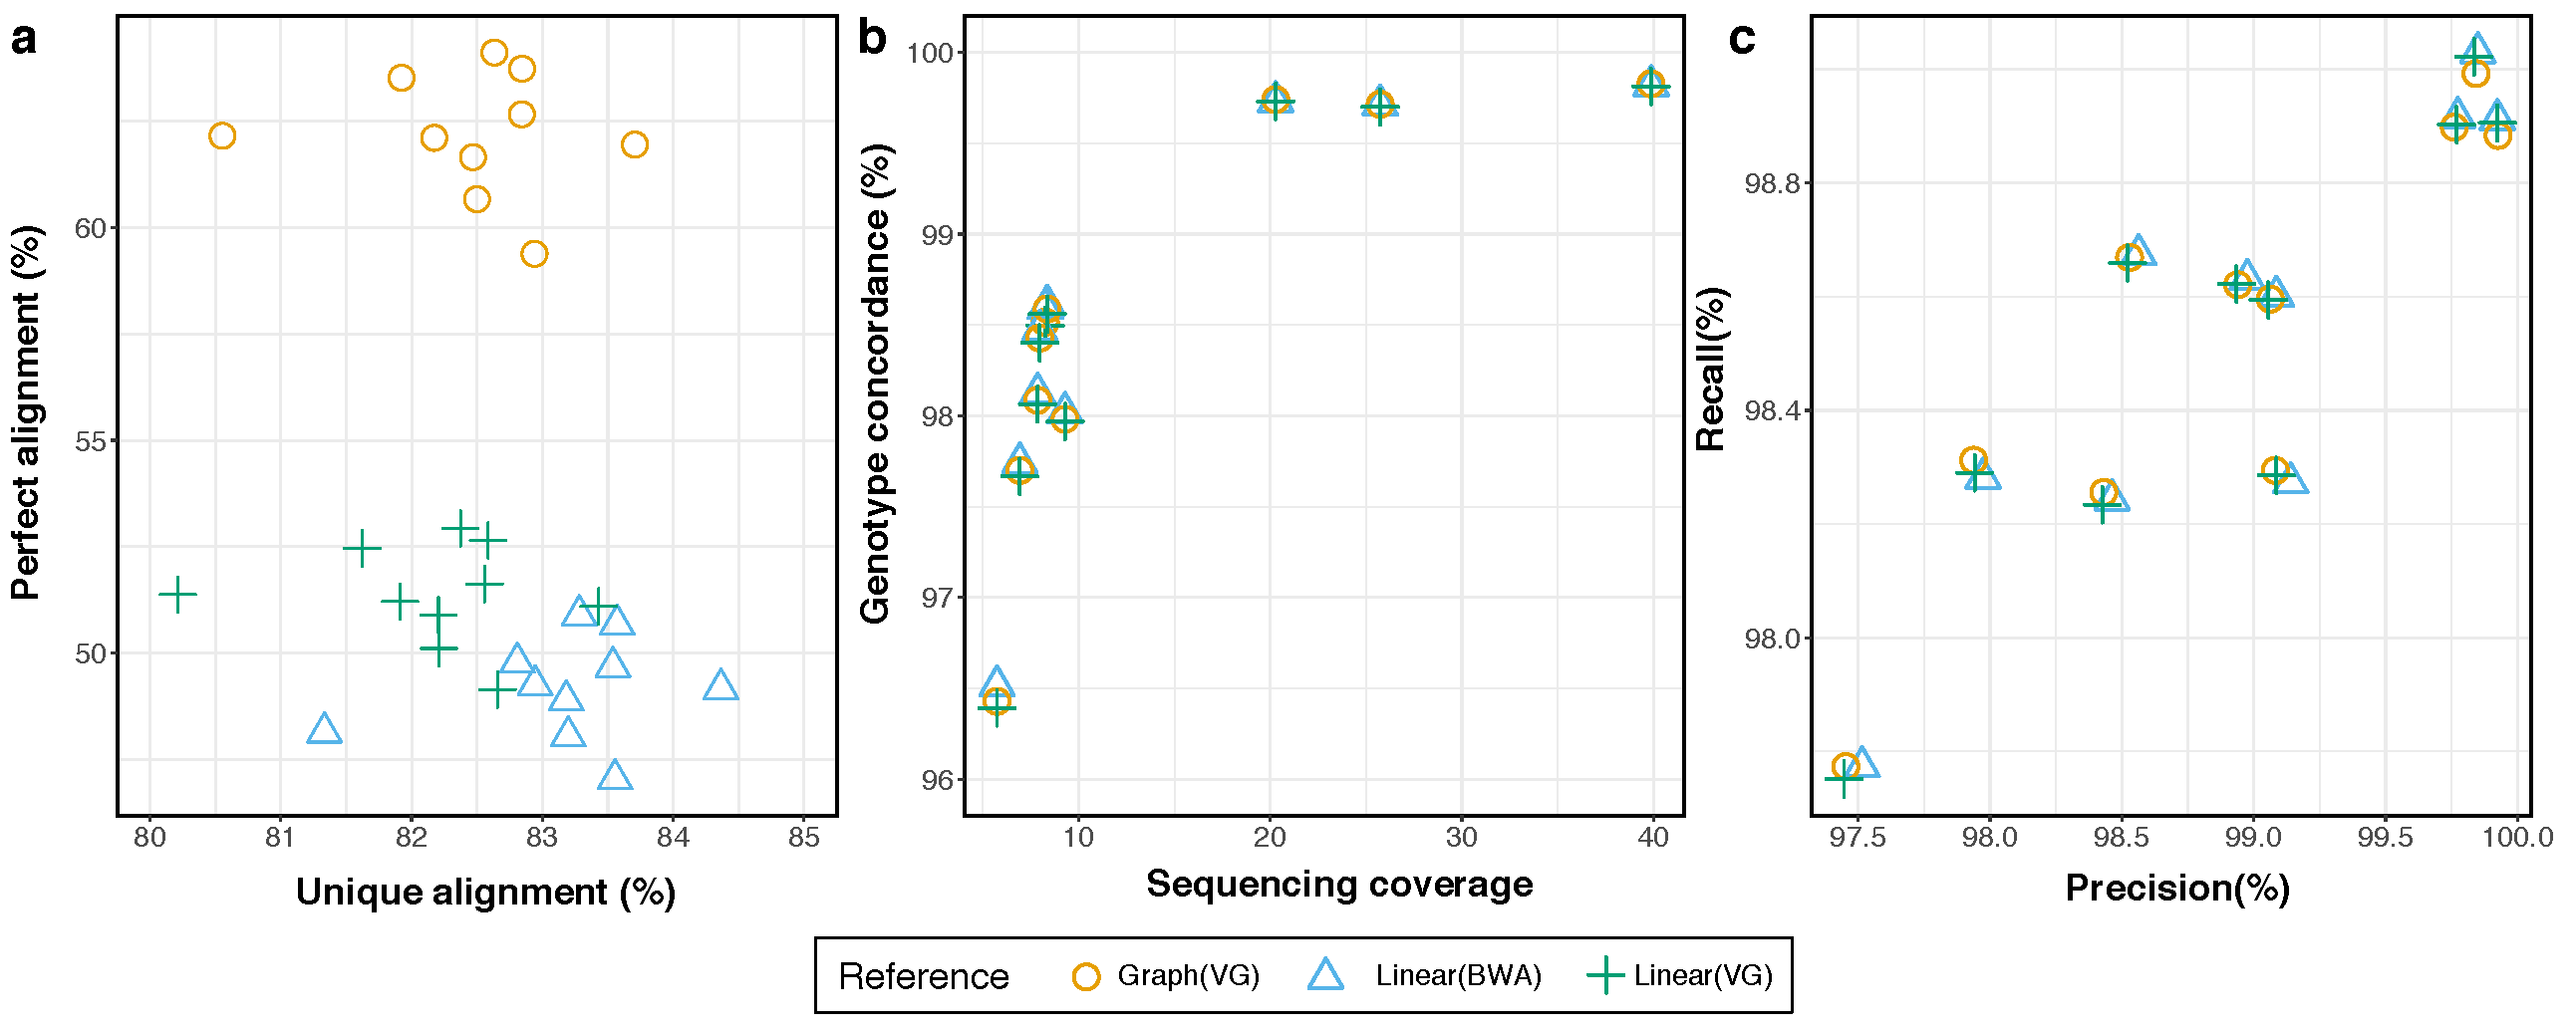
\includegraphics[width=\textwidth]{paper2/main_figure/Fig6.pdf}
    \caption[Sequence read mapping and variant genotyping using a breed-specific augmented whole-genome graph]{\textbf{Sequence read mapping and variant genotyping using a breed-specific augmented whole-genome graph.} 
    \small{\textbf{a} Proportion of sequencing reads that mapped perfectly and uniquely to the BSW-specific augmented (circle) and Hereford-based linear (triangle, cross) reference. \textbf{b} Concordance between sequence variant and corresponding microarray-derived genotypes as a function of sequencing depth. Sequence variant genotypes were obtained using the multi-sample variant calling approach implemented in \emph{SAMtools}. \textbf{c} Corresponding precision-recall statistic. Each symbol represents one BSW animal}}
    \label{fig36:whole}
\end{figure}

We converted (surjected) the graph-based read alignments of 10 BSW cattle to corresponding linear reference coordinates and genotyped polymorphic sites using \emph{SAMtools mpileup}. In order to assess genotyping accuracy, we compared the sequence variant genotypes with array-called genotypes at corresponding positions. Sequence variant genotyping accuracy was correlated with sequencing coverage (Fig. \ref{fig36:whole}b). Genotype concordance, non-reference sensitivity, non-reference discrepancy, and precision did not differ between the graph-based and linear alignments for both raw and hard-filtered genotypes (Fig. \ref{fig36:whole}b, c, Table \ref{sup_tab:s33}). The average concordance, precision and recall from the graph-based alignments was 99.76, 99.84, and 98.93, respectively, for three samples (SAMEA6163185, SAMEA6163188, SAMEA6163187) with sequencing coverage greater than 20-fold. We observed similar values for genotypes called using either \emph{GATK} or \emph{Graphtyper} (Table \ref{sup_tab:s33}). In agreement with our previous findings \citep{crysnanto2019accurate}, genotype concordance was slightly higher using \emph{Graphtyper}, than either \emph{SAMtools} or \emph{GATK}.

\section*{Variation-aware alignment mitigates reference allele bias}

To investigate reference allele bias in genotypes called from linear and graph-based alignments, we aligned sequencing reads of a BSW animal that was sequenced at 40-fold coverage (SAMEA6163185) to either the BSW-specific augmented whole-genome graph or linear reference sequence (Table \ref{sup_tab:s34}). We called genotypes using either \emph{SAMtools mpileup} or \emph{GATK}. The genotypes were filtered stringently to obtain a high-confidence set of 2,507,955 heterozygous genotypes (2,217,069 SNPs and 290,886 Indels, see the \nameref{chap3:meth} section) for reference allele bias evaluation. The BSW-specific augmented whole-genome reference graph contained the alternate alleles at 2,194,422 heterozygous sites (87.49\%).

Using \emph{SAMtools} to genotype sequence variants from variation-aware and linear alignments, the support for reference and alternate alleles was almost equal at heterozygous SNPs (Fig. \ref{fig37:bias}a), indicating that SNPs are not notably affected by reference allele bias regardless of the reference structure. Alternate allele support decreased with variant length for the linear alignments. As expected, bias towards the reference allele was more pronounced at insertion than deletion polymorphisms. For instance, for 456 insertions that were longer than 30 bp, only 26\% of the mapped reads supported the alternate alleles. The allelic ratio of Indel genotypes was closer to 0.5 using graph-based than linear alignments indicating that variation-aware alignment mitigates reference allele bias. However, slight bias towards the reference allele was evident at insertions with length $>$ 12 bp, particularly if the alternate alleles were not included in the graph (Fig. 7a). Inspection of the read alignments using the Sequence Tube Map graph visualization tool \citep{beyer2019sequence} corroborated that the support for alternate alleles is better using graph-based than linear references (Fig. \ref{sup_fig:s314}).

\begin{figure}[!htb]
    \centering
    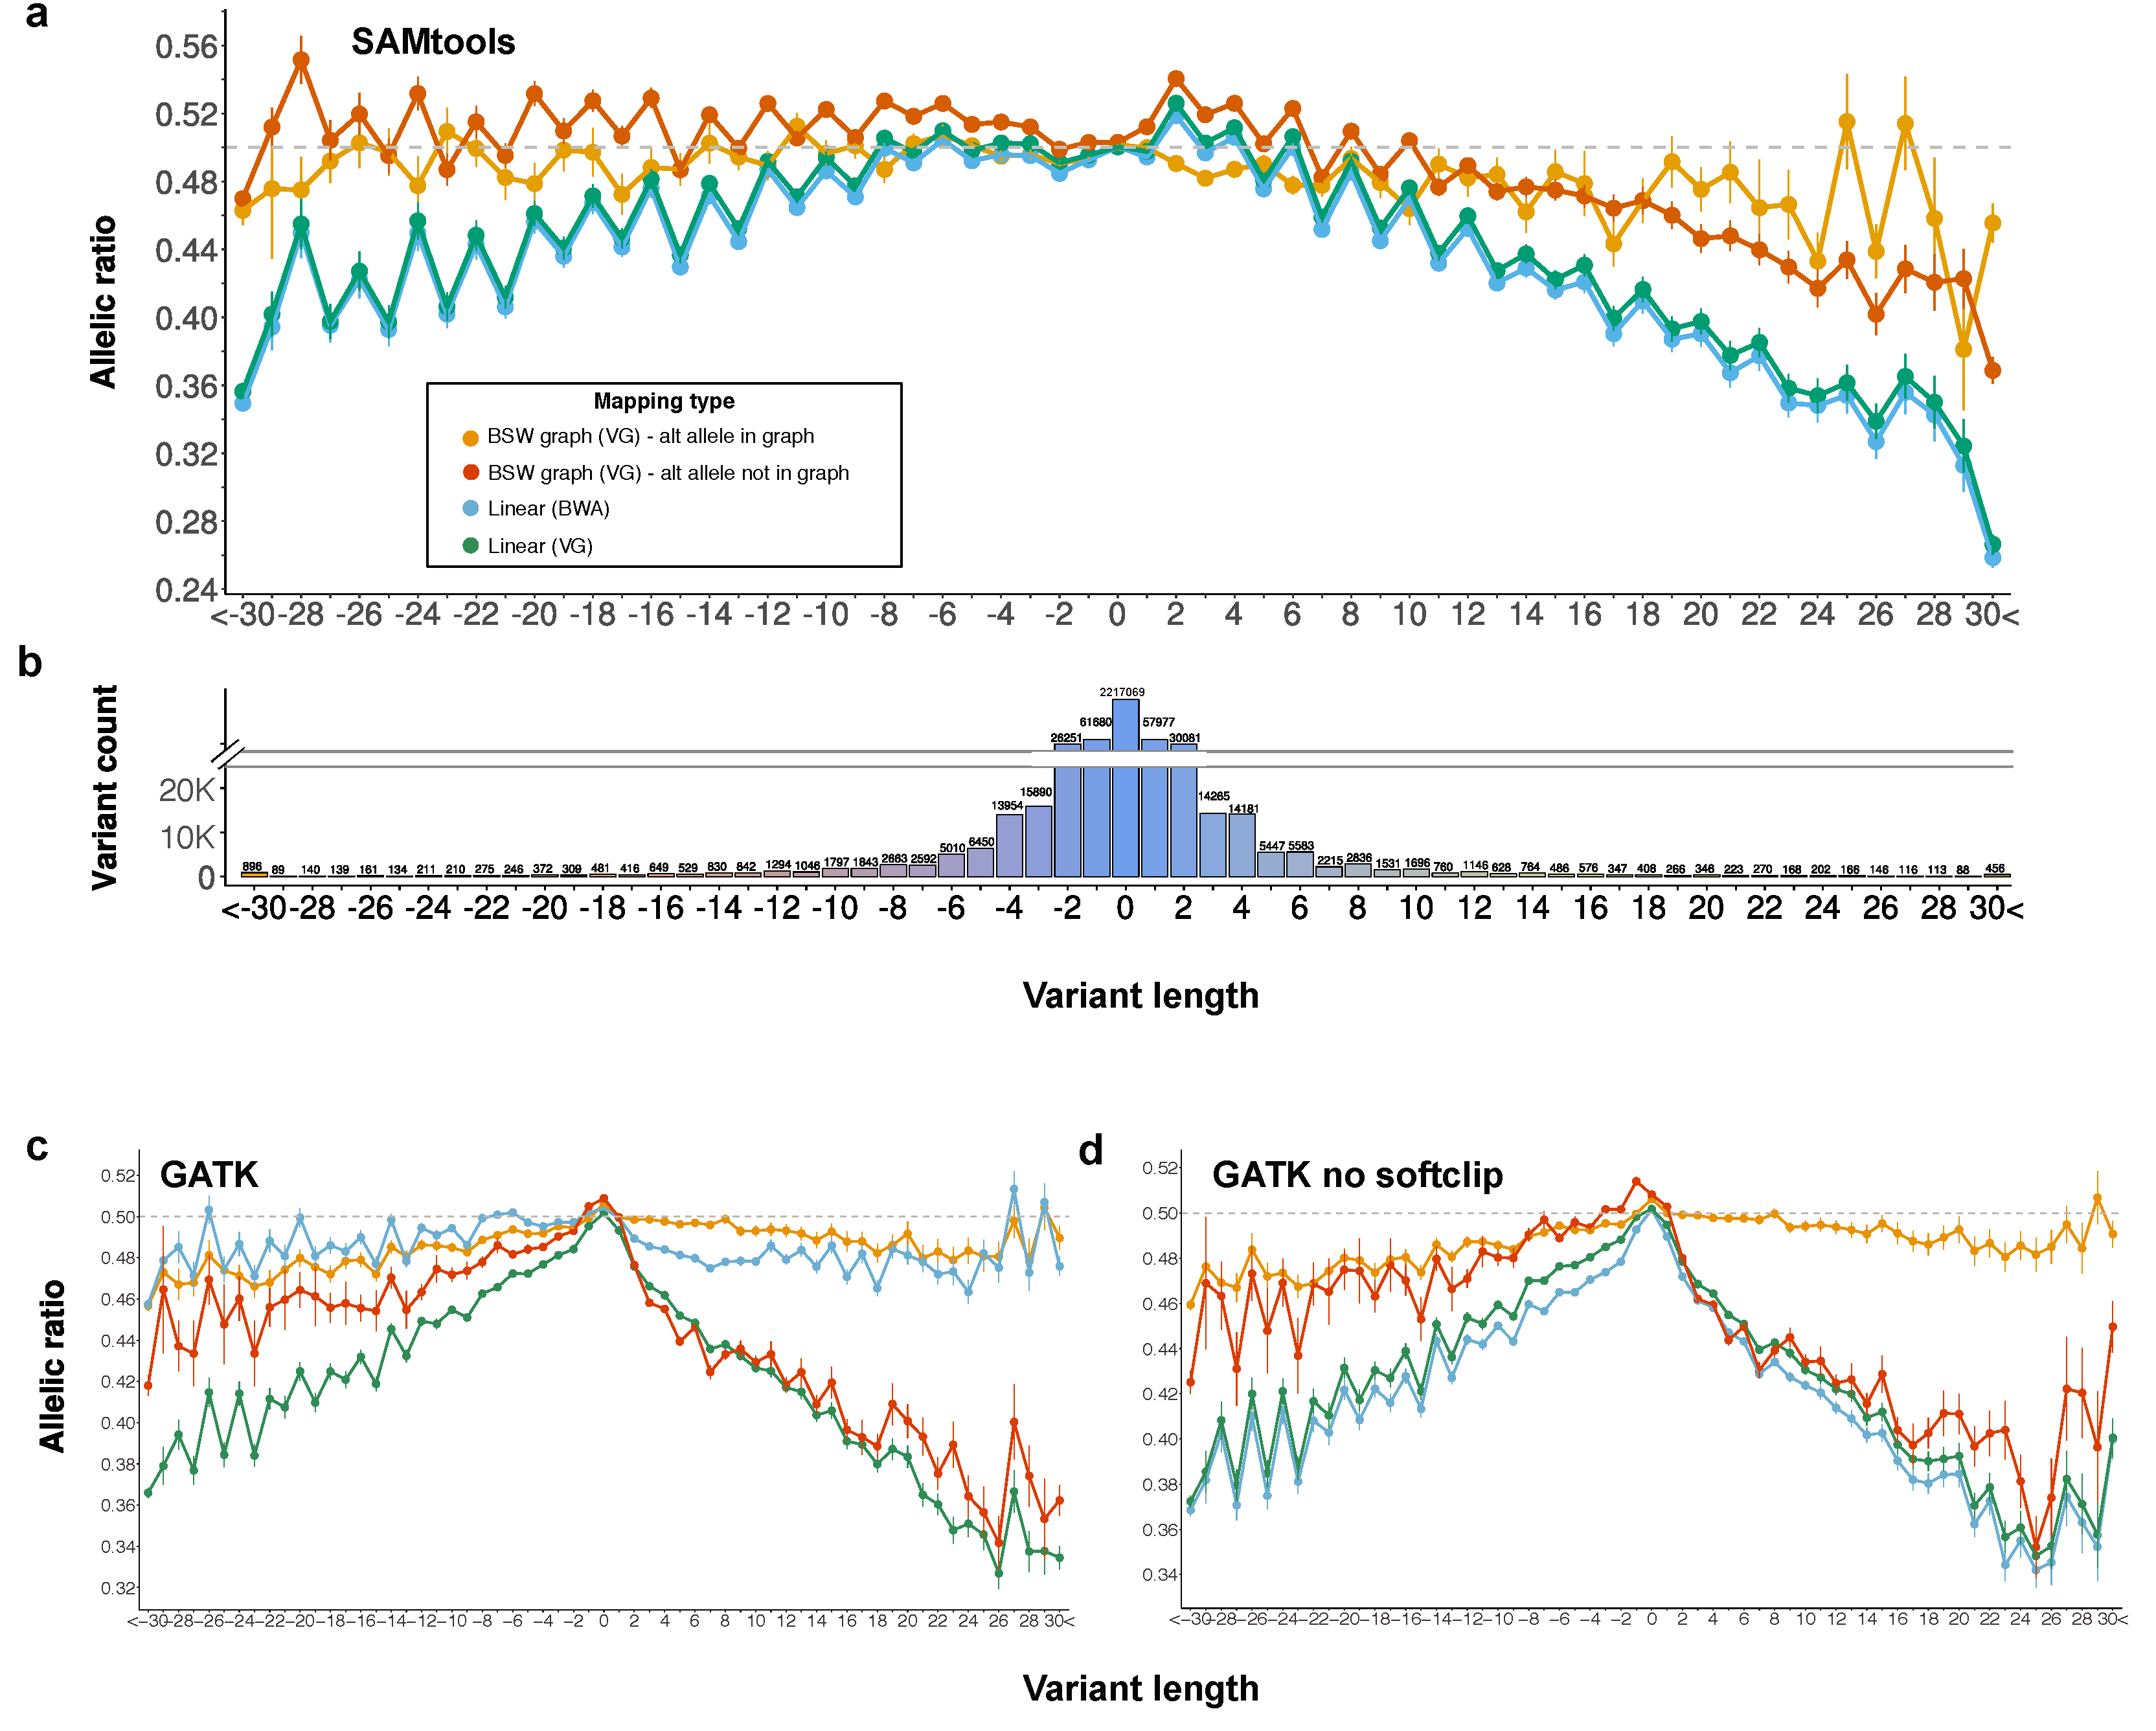
\includegraphics[width=\textwidth]{paper2/main_figure/Fig7.pdf}
    \caption[Reference allele bias from graph-based and linear alignments]{\textbf{Reference allele bias from graph-based and linear alignments.} 
    \small{Reference allele bias from graph-based and linear alignments using \textbf{a} \emph{SAMtools}, \textbf{c} \emph{GATK}, or \textbf{d} \emph{GATK} without soft-clip for variant genotyping and either \emph{BWA mem} or \emph{vg} for alignment. Allelic ratio reflects the proportion of mapped reads supporting the alternate allele. The gray dashed line indicates equal support (0.5) for both alleles. Negative values, zero, and positive values along the \emph{x}-axis represent deletions, SNPs, and insertions respectively. Each dot represents the mean ($\pm$ s.e.m.) allelic ratio for a given variant length. b Number of variants with a given length. To improve the readability, the values above the breakpoint of the y-axis do not scale proportionately with the height of the bars}}
    \label{fig37:bias}
\end{figure}

Both the number of reads mapped and the number of mapped reads supporting alternate alleles was higher at Indels using graph-based than linear alignments (Fig. \ref{sup_fig:s315}). The difference in the number of mapped reads between graph-based and linear alignments increased with variant length. However, the number of mapped reads supporting the reference alleles did not differ between the graph-based and linear alignments. This finding indicates that reduced reference allele bias at Indel genotypes called from graph-based alignments is due to the improved mapping of reads that contain non-reference alleles.

We next investigated if these conclusions also hold for genotypes called by \emph{GATK}. While \emph{SAMtools mpileup} detects variants directly from the aligned reads \citep{li2009sequence}, \emph{GATK HaplotypeCaller} locally realigns the reads and calls variants from the refined alignments \citep{poplin2017scaling}. Using \emph{GATK}, the allelic ratio was close to 0.5 for genotypes called from graph-based alignments across different lengths of variants that were included in the reference graph (Fig. \ref{fig37:bias}c). However, reference allele bias was evident at insertions that were not included in the reference graph. We also observed an almost equal number of reference and alternate alleles at variants genotyped from linear alignments using \emph{GATK}. These findings confirm that the local realignment and haplotype-based genotyping approach of \emph{GATK} might also mitigate reference alleles from linear alignments.

The percentage of soft-clipped reads increased with Indel length in the linear alignments (Fig. \ref{sup_fig:s316}). However, the graph-based alignments contained almost no soft-clipped reads across all Indel lengths. In order to investigate the impact of soft-clipping on variant genotyping, we repeated \emph{GATK} variant discovery and genotyping for the graph-based and linear alignments after all soft-clipped reads were removed (Fig. \ref{fig37:bias}d). As expected, the allelic ratio of genotypes called from the graph-based alignments was not affected by the removal of (very few) soft-clipped reads. However, bias towards the reference allele became evident in genotypes called from linear alignments. This finding confirms that the local realignment of \emph{GATK} rescues Indels that are initially soft-clipped, thus mitigating reference allele bias. This finding also implies that the original pileup information from graph-based alignments facilitates to confidently detect known Indels while avoiding local realignment as implemented in the \emph{GATK HaplotypeCaller}.

\section{Discussion}

To the best of our knowledge, our study is the first to investigate the utility of a variation-aware reference for a species with a gigabase-sized genome other than human. We constructed bovine breed-specific consensus sequences and variation-aware reference graphs using a Hereford-based linear reference sequence as backbone and variants that were filtered for allele frequency in four cattle breeds other than Hereford to investigate read mapping accuracy and variant genotyping from different reference structures.

Using sequencing reads simulated from haplotypes of BSW, FV, OBV, and HOL cattle, our findings confirm that a breed-specific consensus sequence improves linear mapping \citep{ballouz2019time,shukla2019hg19kindel}. However, read mapping is less accurate using linear consensus than variation-aware references that contain pre-selected variants. \citet{grytten2020assessing} reported that an adjusted parameter setting of \emph{BWA mem} and subsequent application of \emph{Minimap2} may further improve the linear mapping accuracy. However, the adjusted linear mapping approach still performs worse than graph-based mapping on reads that contain variants. The accuracy improvements of the adjusted linear mapping approach were small in our study, because the number of sequence variants detected per sample and thus the proportion of reads with variants is almost twice as high in cattle than humans (Table \ref{sup_tab:s31}).

Using a bovine variation-aware reference reduced the proportion of erroneously mapped reads by more than 30\% compared to the most widely used linear mapping approach. A similar improvement in mapping accuracy over the linear reference was achieved for a human variation-aware reference genome \citep{pritt2018forge}. The graph-based alignments using the most accurate breed-specific augmented reference graph contained 0.073\% erroneously mapped reads. Incorrectly mapped reads that had high mapping quality (MQ $>$ 10) were less frequent in the graph-based than linear alignments. Thus, a variation-aware reference may reduce the number of flawed genotypes arising from mapping errors that would remain unnoticed due to high mapping quality. Similar to findings in human genome graphs \citep{pritt2018forge,hickey2020genotyping}, bovine variation-aware references did not improve the mapping of short reads that originate from low-complexity regions.

Our findings demonstrate that variant prioritization is key to accurate variation-aware read mapping. Based on investigations in four genetically distinct cattle breeds and human populations, we make three important observations: first, variation-aware references that contain random variants for which the allele frequency and haplotype phase in the target populations is unknown do not improve read mapping accuracy over linear references. Our previous study also showed that adding many random variants does barely affect sequence variant genotyping from reference graphs \citep{crysnanto2019accurate}. Adding random unphased variants increases the number of alternative alignment paths that are not necessarily biologically plausible haplotypes, thus increasing mapping ambiguity. Second, read mapping accuracy increases approximately linearly with the number of randomly sampled breed-specific variants being added to the genome graph. Similar findings in the four human population-specific augmented graphs confirm that this observation also holds for populations that are strongly enriched for rare alleles and singletons. Third, the highest mapping accuracy at tractable graph complexity can be achieved when variants filtered for allele frequency are added to the graph. Using variant prioritization approaches that are based on allele frequency, we observed the highest mapping accuracy at allele frequency thresholds between 0.01 and 0.10 in four cattle breeds and four human populations. In order to reduce the computational complexity of variation-aware read mapping, previous studies used arbitrarily chosen allele frequency thresholds to prioritize variants to be included in the graphs (e.g., 1\% \citep{garrison2018variation,eggertsson2017graphtyper}, 5\% \citep{maciuca2016natural}, 10\% \citep{kim2019graph}). Using fine-grained allele frequency inclusion thresholds, we find that the read mapping accuracy does not notably differ between the 0.01 and 0.1\% thresholds in most populations. Yet, mapping accuracy declined rapidly for the YRI-specific augmented graph when variants with frequency less than 10\% were added indicating that the optimal inclusion threshold may vary across populations. Variant prioritization approaches that also take into account factors other than allele frequency \citep{pritt2018forge} did not lead to further accuracy improvements in our study. Considering that most cattle breeds have an effective population size between 50 and 200 \citep{hall2016effective,leroy2013methods}, the vast majority of variants with allele frequency greater than 0.1 can be detected from a few sequenced key ancestor animals \citep{jansen2013assessment}. As a matter of fact, key ancestor animals have been sequenced for many cattle breeds \citep{daetwyler2014whole,bouwman2018meta}. Thus, the construction of variation-aware reference structures that are informative for many cattle breeds is readily possible using, e.g., the sequence variant catalog of the 1000 Bull Genomes Project \citep{daetwyler2014whole,hayes20191000}.

A pan-genome graph that contained variants filtered for allele frequency across the four cattle breeds enabled almost similar accuracy improvements over the linear reference than breed-specific augmented graphs (Fig. \ref{fig34:breed}b). Although the principal component analysis confirmed that the breeds considered in our study are genetically distinct populations, they share many common alleles. Moreover, compared to human populations, the proportion of rare alleles and singletons is low in cattle. The bovine pan-genome graph constructed in our study contained between 75.28 and 80.82\% of the variants that were also added to the breed-specific augmented graphs. Instead of building many breed-specific graphs, the construction of a universal pan-genome graph is likely possible without notably compromising the accuracy of read mapping. This conclusion may hold for many species with genetically distinct sub-populations that share common alleles. Compared to the linear reference, the mapping accuracy was also significantly higher when reads from one breed were mapped to a genome graph that contained variants filtered for allele frequency in another somewhat related breed. Thus, the BSW-specific augmented whole-genome graph constructed in our study will likely improve read mapping accuracy over the linear reference and mitigate reference allele bias also for breeds other than BSW, FV, HOL, and OBV. Our BSW-specific augmented whole-genome graph is available at \url{https://doi.org/10.5281/zenodo.3759712} \citep{Crysnanto2020data}. In order to facilitate the construction of variation-aware reference structures, the entire workflow to establish whole-genome graphs is also available at \url{https://github.com/danangcrysnanto/bovine-graphs-mapping}.

The number of sequencing reads that aligned to the BSW-specific whole-genome graph with full identity increased considerably ($+$ 13\%) over the linear reference sequence at the cost of a slightly reduced ($−$ 0.72\%) number of unique alignments. A two-step graph alignment approach that exploits a refined search space might reduce the number of multiple mappings in dense variation-aware graphs \citep{grytten2020assessing}. Compared to a human whole-genome graph, the improvement in perfect mapping over the linear reference was slightly larger in our bovine whole genome graph (9.2\%) \citep{garrison2018variation}. However, the proportion of reads with perfect alignments (62.19\%) was lower in our BSW-specific whole-genome graph, likely because it contained only sequences that were assembled to the 29 autosomes. The graph did not contain 269.77 Mb of the sex chromosomes, mitochondrial DNA, and 2180 unplaced contigs. A more sophisticated assembly of the bovine genome with increased continuity particularly at the sex chromosomes \citep{rice2020continuous,liu2019new} might serve as a backbone for an improved variation-aware genome graph.

In order to detect SNPs and Indels from the variation-aware reference graph using widely used sequence variant genotyping methods, we had to make the graph-based alignments compatible with linear coordinates. Thus, our assessment of sequence variant genotyping from the bovine whole-genome graph is based on surjected graph-based alignments. It is possible that converting graph-based to linear alignments compromises variant discovery. However, the accuracy and sensitivity of genotyping did not differ between graph-based and linear alignments indicating that our whole-genome graph facilitates accurate sequence variant (SNPs and small Indels) genotyping. It is worth noting that our analysis considered only SNPs that are located in well-accessible regions of the genome, thus possibly overestimating genotyping accuracy \citep{li2014toward,malomane2018efficiency}. A benchmark dataset that enables unbiased evaluation of sequence variant genotyping \citep{li2018synthetic} is not available for the four cattle breeds considered in our study. Because approximately 90\% of the considered SNPs were already included in the BSW-specific whole-genome graph, they can be detected and genotyped easily from graph-based alignments \citep{paten2017genome}. These variants can also be detected and genotyped accurately from linear alignments \citep{crysnanto2019accurate,zook2019open}.

As expected, bias towards the reference allele was less in graph-based than linear alignments particularly at variants that were included in the graph. Unbiased genotyping of heterozygous variants from graph-based alignments is possible because reads supporting alternate alleles align better to variation-aware than linear references. Thus, our bovine whole-genome graph offers an appealing novel reference for investigations that either rely on low-coverage sequencing or are sensitive to unbiased allele frequencies \citep{van2015wasp,gunther2019presence,rozowsky2011alleleseq}. Because a benchmark dataset for an unbiased evaluation of sequence variant genotyping performance \citep{li2018synthetic} is not available in cattle, our assessment was restricted to heterozygous variants that were identified from both linear and graph-based alignments. This set of variants is possibly enriched for variants that can be called confidently from linear alignments, thus underestimating the graph-based genotyping performance (e.g., \citep{garrison2018variation}).

Our study has three limitations. First, variants used to construct the breed-specific augmented genome graphs might be biased because they were detected from linear alignments of short sequencing reads. Variant discovery from an independent variation-aware reference structure might allow for a more complete assessment of genetic variation \citep{li2018synthetic}. Second, we used the Hereford-based linear reference sequence as backbone to construct breed-specific augmented reference sequences. However, the Hereford-based reference sequence might lack millions of basepairs that segregate in the four breeds considered in our study \citep{sherman2019assembly,hehir2016high,holden2018assembly,li2010building}. These nucleotides are likely missing in the breed-specific augmented reference graphs constructed in our study. Accurate and continuous genome assemblies from BSW, FV, HOL, and OBV cattle are not available. All bovine genome assemblies that are available to date had been compiled from individuals that are distantly related to the breeds in our study \citep{koren2018novo,rice2020continuous,rosen2020novo}. Haplotype-resolved genome assemblies of cattle from different breeds will facilitate the construction of more informative genome graphs and make non-reference sequences and their sites of variation amenable to genetic investigations \citep{koren2018novo,rice2020continuous}. Third, we did not investigate the impact of large sequence variation on sequence read mapping and variant genotyping performance because neither a high-quality benchmark set of large structural variants (cf. \citep{chaisson2019multi}) nor long-read sequencing data is available for the four cattle breeds considered. Adding insertion and deletion polymorphisms detected from short-read sequencing data did not lead to accuracy improvements in our study likely because structural variants detected from short reads are notoriously biased and incomplete \citep{alkan2011genome}. Recent studies indicated that large structural variants can be identified accurately from genome graphs \citep{hickey2020genotyping,eggertsson2019graphtyper2,chen2019paragraph,rakocevic2019fast}. Eventually, a bovine genome graph that unifies multiple breed-specific haplotype-resolved genome assemblies and their sites of variation might provide access to sources of variation that are currently neglected when short sequencing reads are aligned to a linear reference sequence \citep{duan2019hupan,beyter2020long,li2020design}.

\section{Conclusions}
We constructed the first variation-aware reference graph for \emph{Bos taurus} that improves read mapping accuracy over the linear reference sequence. The use of this novel reference structure facilitates accurate and unbiased sequence variant genotyping. Our results indicate that the construction of a widely applicable bovine pan-genome graph is possible that enables accurate genome analyses for many diverged breeds.


\section{Methods}
\label{chap3:meth}

\subsection*{Whole-genome sequencing data}

We used short paired-end sequencing reads of 288 cattle from dairy (n $=$ 82 Brown Swiss (BSW), n $=$ 49 Holstein (HOL)) and dual-purpose (n $=$ 49 Fleckvieh (FV), n $=$ 108 Original Braunvieh (OBV)) breeds to detect variants that segregate in these populations. The average sequencing depth of the 288 cattle was 12.71-fold, and it ranged from 3.49 to 70.04. Most of the sequencing data were generated previously \citep{daetwyler2014whole,crysnanto2019accurate,jansen2013assessment,baes2014evaluation,hofstetter2019non}. Accession numbers for all animals are available in Table \ref{sup_tab:s34}.

We trimmed adapter sequences from the raw data and discarded reads for which the phred-scaled quality was below 15 for more than 15\% of the bases using fastp \citep{chen2018fastp}. Subsequently, the sequencing reads were aligned to the linear reference assembly of the bovine genome (ARS-UCD1.2, GCF\_002263795.1) using \emph{BWA mem} \citep{li2013aligning}. 
Duplicates were marked and the aligned reads were coordinate sorted using the Picard tools software suite (\url{http://broadinstitute.github.io/picard}) and Sambamba \citep{tarasov2015sambamba}, respectively. We discovered and genotyped polymorphic sites from the linear read alignments using the Best Practices Workflow descriptions for multi-sample variant calling with \emph{GATK} (version 4.1.0) \citep{depristo2011framework}. Because a truth set of variants required for variant quality score recalibration (VQSR) is not available for Bos taurus, we followed the recommendations for sequence variant discovery and filtration when applying VQSR is not possible. Genotypes of the hard-filtered variants were subsequently refined, and sporadically missing genotypes were imputed with \emph{BEAGLE} v4 \citep{browning2016genotype} using the genotype likelihoods from the \emph{GATK HaplotypeCaller} model as input values. Additional information on the sequence variant genotyping workflow and the expected genotyping accuracy can be found in \citet{crysnanto2019accurate}. Nucleotide diversity was calculated in non-overlapping 10 kb windows separately for each breed using the $\pi$ (nucleotide diversity) module implemented in the \emph{vcftools} software \citep{danecek2011variant}.

We discovered and genotyped large structural variants ($>$ 50 bp) including insertions, deletions, inversions, duplications, and translocations in 82 sequenced BSW animals using \emph{Delly} v0.7.8 \citep{rausch2012delly} with the default settings. We retained only insertion and deletion variants that had been refined using split-reads (PRECISE-flag in the vcf file).

The principal components of a genomic relationship matrix constructed from whole-genome sequence variant genotypes were calculated using PLINK v1.9 \citep{chang2015second}. The top principal components separated the animals by breeds, corroborating that the four breeds are genetically distinct (Fig. \ref{fig32:freq}a). To take haplotype diversity and different linkage disequilibrium phases across breeds into account, the sequence variant genotypes were phased for each breed separately using \emph{BEAGLE} v5 \citep{browning2018one}.

Unless stated otherwise, our analyses included 541,876 biallelic SNPs and Indels that were detected on bovine chromosome 25. The \emph{vg toolkit} version 1.17.0 “Candida” \citep{garrison2018variation} was used for all graph-based analyses.

\subsection*{Haplotype-aware simulation of short sequencing reads}


We simulated 10 million reads (150 bp) from reference haplotypes of one animal per breed that had sequencing coverage greater than 20-fold (see Table \ref{sup_tab:s34}). Therefore, we added the phased sequence variants of each of the four animals to the linear reference to construct individualized reference graphs using \emph{vg construct}. The haplotype-aware indexes of the resulting graphs were built using \emph{vg index xg} and \emph{gbwt}. \emph{vg paths} and \emph{vg mod} were used to extract the haplotype paths from the individualized reference graphs. Subsequently, we simulated 2.5 million paired-end reads (2 × 150 nt) from each haplotype using \emph{vg sim}, yielding 10 million 150 bp reads per breed corresponding to approximately 35-fold sequencing coverage of bovine chromosome 25. The simulation parameter setting for read and fragment length was 150 and 500 ($\pm$ 50), respectively. The substitution and indel error rate was 0.01 and 0.002, respectively, according to the settings used in \citet{garrison2018variation}.

\subsection*{Read mapping to graphs augmented with variants filtered for allele frequency}

The alternate allele frequency of 541,876 variants of bovine chromosome 25 was calculated separately for the BSW, FV, HOL, and OBV breeds using sequence variant genotypes of 82, 49, 49, and 108 sequenced cattle, respectively. We added to each breed-specific genome graph 20 sets of variants that were filtered for alternate allele frequency using thresholds between 0 and 1 with increments of 0.01 and 0.1 for frequency below and above 0.1, respectively. For instance, at an alternate allele frequency threshold of 0.05, the graph was constructed with variants that had alternate allele frequency greater than 5\%. Alleles that were only detected in the four animals used to simulate reads (see above) were not added to the breed-specific augmented genome graphs.

The four breed-specific augmented genome graphs contained the same number of variants at a given allele frequency threshold to ensure that their density of information was similar. The number of variants added to the graphs was determined according to the breed in which the fewest variants were detected at a given allele frequency threshold. For the other three breeds, we sampled randomly from all variants that were detected at the respective alternate allele frequency threshold. We indexed the breed-specific augmented graphs using \emph{vg} index to obtain the topological (\emph{xg}), query (\emph{gcsa}), and haplotype (\emph{gbwt}) index. Eventually, the simulated reads were aligned to the breed-specific augmented reference graphs using \emph{vg map} with default mapping parameter settings considering both graph (\emph{xg}, \emph{gcsa}) and haplotype (\emph{gbwt}) indexes.

To compare the accuracy of read mapping between variation-aware and linear reference structures, the simulated reads were also aligned to the linear reference sequence of bovine chromosome 25 using either \emph{BWA mem} with default parameter settings or \emph{vg map}. To enable linear mapping with \emph{vg map}, we constructed an empty graph (without adding any sequence variants) from the linear reference sequence.

\subsection*{Read mapping to human population-specific augmented genome graphs}

We downloaded phased whole-genome variants of 2504 individuals from phase 3 of the 1000 Genomes Project \citep{10002015global} as well as the corresponding reference sequence (g1k\_v37; \url{https://www.internationalgenome.org/category/reference/}). We selected four populations which we considered to be genetically distinct based on the results of a principal components analysis and for which the number of individuals was similar to the number of individuals for the four cattle breeds, i.e., GBR (British in England and Scotland, European), YRI (Yoruba in Ibadan Nigeria, African), JPT (Japanese in Tokyo, East Asia), and STU (Sri Lankan Tamil, South Asia). The principal components were calculated from a genomic relationship matrix constructed using 81.27 million autosomal variants using the \emph{PLINK} (v1.9) software \citep{chang2015second}. Alternate allele frequency was calculated separately for the four populations for all variants of human chromosome 19. Nucleotide diversity was calculated with the \emph{vcftools} software as detailed above. In order to construct population-specific augmented genome graphs, we used the reference sequence (g1k\_v37) of human chromosome 19 as a backbone and added variants filtered for alternate allele frequency in the four populations (following the approach explained above). For each population, we constructed 20 graphs that contained between 3153 and 290,593 variants. We simulated 10 million paired-end reads for each population from reference haplotypes (as detailed above) of four selected samples (GBR: HG00096, YRI: NA18486, JPT: NA18939, STU: HG03642). The simulated reads were then mapped to the population-specific augmented genome graphs using the \emph{vg toolkit}.

\subsection*{Read mapping to bovine breed-specific augmented graphs}

We simulated 10 million reads from the haplotypes of a BSW animal (SAMEA6272105) and mapped them to variation-aware reference graphs that were constructed using variants (SNPs and Indels) filtered for alternate allele frequency greater than 0.03. Alleles that were only detected in SAMEA6272105 were excluded from the graphs. All graphs contained 243,145 variants. The number of variants was determined according to the HOL cattle breed because the lowest number of variants segregated at an alternate allele frequency greater than 0.03 in that breed. To investigate the utility of targeted genome graphs, we mapped the simulated BSW reads to a graph that contained variants filtered for allele frequency in BSW cattle. To investigate across-breed mapping, we mapped the simulated BSW reads to graphs that contained variants filtered for allele frequency in either FV, HOL, or OBV cattle. We also mapped the BSW reads to a bovine pan-genome graph that contained variants that were filtered for allele frequencies across the four cattle breeds. Additionally, we investigated the accuracy of mapping reads to a graph that was built from randomly selected variants. To construct the random graph, we randomly sampled from 2,294,416 variants that were detected on bovine chromosome 25 from animals of various breeds of cattle (\url{http://www.1000bullgenomes.com/doco/ARS1.2PlusY_BQSR_v2.vcf.gz}). The allele frequencies and haplotype phases of the random variants were not known. We constructed personalized graphs that contained only variants and haplotypes that were detected in the animals used for read simulation. The variation-aware graphs were subsequently indexed using \emph{vg index} (see above). The simulated BSW reads were mapped to the different graphs using \emph{vg map} (see above). The construction and indexing of graphs as well as read simulation and mapping were repeated ten times. We report in the main part of the paper the average values of ten replicates. This entire procedure was repeated with reads that were simulated from the haplotypes of FV (SAMN02671626), HOL (SAMN02671584), and OBV animals (SAMEA5059743).

\subsection*{Read mapping to consensus reference sequences}

We modified alleles of the ARS-UCD1.2 linear reference sequence using the vcf2diploid tool \citep{rozowsky2011alleleseq}. We created two adjusted linear reference sequences for bovine chromosome 25:

\begin{itemize}
    \item \emph{major-BSW}: 67,142 nucleotides of the linear reference sequence were replaced with the corresponding major alleles detected in 82 BSW cattle.
    \item \emph{major-pan}: 73,011 nucleotides of the linear reference sequence were replaced with the corresponding major alleles detected in 288 cattle from four breeds.
\end{itemize}

Ten million BSW reads were simulated (see above) and mapped to the original and modified linear reference sequences, as well as the corresponding variation aware reference structures using either \emph{BWA mem} or \emph{vg map} (see above) with default parameter settings. Since the replacement of reference alleles with Indels causes a shift in the reference coordinate system, we converted the coordinates of simulated reads between the original and modified reference using a local instance of the \emph{UCSC liftOver} tool \citep{haeussler2019ucsc} that was guided using a chain file produced by \emph{vcf2diploid}. In order to prevent possible errors arising from coordinate shifts when reference nucleotides are either deleted or inserted at Indels, we repeated the analysis when only the alleles at SNPs were replaced.

\subsection*{Assessment of the read mapping accuracy}

We used \emph{vg stats} to obtain the number of nodes and edges, biologically plausible paths and length for each variation-aware reference graph. To assess the accuracy of graph-based alignment, we converted the Graph Alignment Map (GAM)-files to JavaScript Object Notation (JSON)-files using \emph{vg view}. Subsequently, we applied the command-line JSON processor jq (\url{https://stedolan.github.io/jq/}) to extract mapping information for each read. Mapping information from linear alignments were extracted from the Binary Alignment Map (BAM)-files using the Python module \emph{pysam} (version 0.15.3) (\url{https://github.com/pysam-developers/pysam}).

Using \emph{vg annotate}, we annotated the simulated reads with respect to the linear reference coordinates and determined if they contained non-reference alleles. Comparing the true and mapped positions of the simulated reads enabled us to differentiate between correctly and incorrectly mapped reads. Following the approach of \citet{garrison2018variation} and taking into account the possibility that aligned reads may be clipped at Indels, we considered reads as incorrectly mapped if their starting positions were more than $k$ $=$ 150 ($k$ $=$ read length) bases distant from true positions. The functional relevance genomic regions where the simulated reads originated from were determined based on the \emph{Ensembl} annotation (version 99, \citep{yates2020ensembl}) of the bovine ARS-UCD 1.2 reference sequence. The coordinates of repetitive elements were determined based on RepeatMasker \citep{smith2013repeatmasker} annotation tables of the \emph{UCSC} Genome Browser.

In order to assess mapping sensitivity and specificity, we calculated the cumulative TPR (true$-$positive rate) and FPR (false$-$positive rate) at different mapping quality thresholds and visualized it as pseudo-ROC (receiver operating characteristic) curve \citep{garrison2018variation} using:

\[TPR_i=\frac{\sum_{i}^{60}TP_k}{n}\]
\[FPR_i=\frac{\sum_{i}^{60}FP_k}{n}\]

where $TP_i$ and $FP_i$ represent the number of correctly and incorrectly mapped reads, respectively, at a given phred-scaled mapping quality threshold i (60, 50, 40, 30, 20, 10, 0), and $n$ is the total number of reads mapped.

\subsection*{Read mapping and sequence variant genotyping from bovine whole-genome graph}

Using 14,163,824 autosomal biallelic variants (12,765,895 SNPs and 1,397,929 Indels) that had alternate allele frequency greater than 0.03 in 82 BSW cattle, we constructed a BSW-specific augmented whole-genome graph. The Hereford-based linear reference sequence (ARS-UCD1.2) was the backbone of the graph. Specifically, we constructed graphs for each of the 29 autosomes separately using \emph{vg construct}. Subsequently, \emph{vg ids} was run to ensure that the node identifiers were unique in the concatenated whole-genome graph. We removed complex regions from the whole-genome graph using \emph{vg prune} with default parameter settings and built the topological (\emph{xg}) and query (\emph{gcsa}) index for the full and pruned graph, respectively, using \emph{vg index}. The haplotype paths of the 82 BSW cattle obtained using \emph{BEAGLE} v5 (see above) were provided using a \emph{gbwt} index.

To evaluate sequence variant genotyping from the whole-genome graph, we used between 122,753,846 and 904,047,450 million paired-end (2 × 150 bp) sequencing reads from 10 BSW cattle (SAMEA6163185, SAMEA6163188, SAMEA6163187, SAMEA6163177, SAMEA6163178, SAMEA6163176, SAMEA6163179, SAMEA6163183, SAMEA6163181, SAMEA6163182, Table \ref{sup_tab:s34}) that had been sequenced at between 5.74 and 39.88-fold genome coverage. These animals were not part of the 82 BSW animals that were used to detect the variants that were added to the graph. We trimmed adapter sequences and removed reads that had more than 20\% bases with phred-scaled quality less than 20 using \emph{fastp} \citep{chen2018fastp}. Subsequently, we mapped the pruned reads to either the BSW-specific augmented whole-genome graph or the linear reference sequence using either \emph{vg map} while supplying both graph (\emph{xg}, \emph{gcsa}) and haplotype (\emph{gbwt}) index to produce GAM files for each sample or \emph{BWA mem}. To make the coordinates of the graph-based alignments compatible with linear reference coordinates, we converted the GAM- to BAM-files using \emph{vg surject}. Variants were detected and genotyped from the surjected files using the multi-sample variant calling approach of either \emph{GATK} \citep{poplin2017scaling}, \emph{Graphtyper} \citep{eggertsson2017graphtyper}, or \emph{SAMtools} \citep{li2009sequence}, as stated above and detailed in \citep{crysnanto2019accurate}.

In order to assess the read mapping accuracy from real sequencing data, we calculated the proportion of reads that aligned (i) perfectly and (ii) uniquely \citep{pritt2018forge,shukla2019hg19kindel,novak2017genome}. A read was considered to map perfectly if the edit distance was zero along the entire read (NM:0 tag in \emph{BWA mem}-aligned BAM files; identity 1 in \emph{vg map}-aligned GAM-files), and without hard clipping (H tag) or soft clipping (S tag) in CIGAR string. A read was considered to map uniquely if either a single primary alignment was reported for the respective read or reads that had secondary alignments (XA tag in \emph{BWA mem}-aligned BAM files; secondary\_score $>$ 0 in \emph{vg map}-aligned GAM-files) had one alignment with phred-scaled mapping quality score of 60.

The sequenced BSW animals also had Illumina SNP BeadChip-derived genotypes at between 24,512 and 683,752 positions. The sequence variant genotypes were compared to microarray-called genotypes at corresponding positions to calculate recall/non-reference sensitivity, genotype concordance, precision, and non-reference discrepancy \citep{depristo2011framework,linderman2014analytical}. The concordance metrics are explained in Fig. \ref{sup_fig:s317}.

Snakemake workflows \citep{koster2012snakemake} for whole-genome graph construction, read mapping, and variant discovery are available in the \emph{Github} repository (\url{https://github.com/danangcrysnanto/bovine-graphs-mapping}).

\subsection*{Assessment of reference allele bias}

Reference allele bias was assessed at the heterozygous genotypes that had been detected in a BSW animal (SAMEA6163185) that had been sequenced at high (40-fold) coverage. Raw sequencing data were filtered as stated above and aligned to either the linear reference sequence or BSW-specific augmented genome graph using \emph{BWA mem} and \emph{vg map}, respectively. Sequence variant genotypes were discovered and genotyped from either surjected graph-based or linear alignments using the single sample variant calling approaches implemented in either \emph{GATK HaplotypeCaller} or \emph{SAMtools mpileup}. Variants were filtered using quality by depth (QD) $>$ 10, mapping quality (MQ) $>$ 40, and minimum read depth (DP) greater than 25 to ensure confident genotype calls and sufficient support for reference and alternate alleles at heterozygous genotypes. We considered only variants that were detected from both graph-based and linear alignments. At each heterozygous genotype, we quantified the number of reads supporting alternate and reference alleles using allelic depth information from the vcf files.

\subsection*{Availability of data and materials}

The scripts and data used in this study are available via \emph{GitHub} repository (\url{https://github.com/danangcrysnanto/bovine-graphs-mapping}) and archived in Zenodo (data: \url{https://doi.org/10.5281/zenodo.3759712} \citep{Crysnanto2020data} and scripts: \url{https://doi.org/10.5281/zenodo.3763286} \citep{Crysnanto2020script}). Raw sequencing read data of 298 cattle used for graph construction, evaluation of variant genotyping accuracy, and assessment of reference allele bias are available at the European Nucleotide Archive (ENA) (\url{http://www.ebi.ac.uk/ena}) with study accession of PRJNA238491 \citep{daetwyler2014whole}, PRJEB28191 \citep{crysnanto2019accurate}, and PRJEB18113 \citep{hofstetter2019non}. Detailed accession numbers for each sample are provided in Table \ref{sup_tab:s34}. \\

\vspace{-2em}
% \let\Origclearpage\clearpage
% \let\clearpage\relax


\singlespacing
\footnotesize

% \bibliographystyle{abbrvnat}
\bibliographystyle{unsrtnat}
\bibliography{references/chapter3_ref}
%\printbibliography[title=References]

% \let\clearpage\Origclearpage

\ifdefined\BuildingFromMainFile
\else
   \end{document}
\fi

\iftwoside
\cleardoublepage
\newpage
\fi

\chapter[Bovine multi-assembly graphs]{\LARGE{Analysis of the bovine multi-assembly graphs}}
\label{chap:multigraph}

\subsection*{Preface: Bridging text between Chapter 3 and Chapter 4}

\normalsize
This chapter investigated the utility of multi-assembly graphs that integrated the collection of genome assemblies into a unified representation. The first bovine multi-assembly graph was constructed that unified six cattle assemblies, including its close relatives of Brahman and Yak using the \emph{minigraph} software. The application of the multi-assembly graph identified the 70 Mb sequences not included in the existing \emph{Bos taurus} reference genome. Further analysis showed that these non-reference sequences contain abundant functionally relevant sequences. \\

\bigskip

\begin{center}\fbox{\begin{minipage}{35em}

% \emph{Contribution}: Hubert Pausch and I conceived the study. Zih-Hua Fang coordinated the sampling and long-read sequencing. Alexander Leonard assembled the Original Braunvieh genome. Hubert Pausch, Alexander Leonard, and I performed the analyses and wrote the manuscript. 

\emph{Contribution}: I participated in conceiving the study, analysing the results and writing the manuscript. I wrote the multi-assembly graph pipelines. 


\end{minipage}}\end{center}

\onehalfspacing
\ifdefined\BuildingFromMainFile
\else
   \documentclass[../main.tex]{subfiles}
   \begin{document}
\fi


\graphicspath{{figure/}{../figure/}}

\onehalfspacing
\normalsize


\begin{abstract}   
\onehalfspacing
\small
Many genomic analyses start by aligning sequencing reads to a linear reference genome. However, linear reference genomes are imperfect, lacking millions of bases of unknown relevance, and are unable to reflect the genetic diversity of populations. This makes reference-guided methods susceptible to reference-allele bias. To overcome such limitations, we build a pangenome from six reference-quality assemblies from taurine and indicine cattle as well as yak. The pangenome contains an additional 70,329,827 bases compared to the \emph{Bos taurus} reference genome. Our multi-assembly approach reveals 30 and 10.1 million bases private to yak and indicine cattle, respectively, and between 3.3 and 4.4 million bases unique to each taurine assembly. Utilizing transcriptomes from 56 cattle, we show that these non-reference sequences encode transcripts that hitherto remained undetected from the \emph{Bos taurus} reference genome. We uncover putative genes, primarily encoding proteins contributing to immune response and pathogen-mediated immunomodulation, differentially expressed between \emph{Mycobacterium bovis}-infected and non-infected cattle that are also undetectable in the \emph{Bos taurus} reference genome. Using whole-genome sequencing data of cattle from five breeds, we show that reads which were previously misaligned against the \emph{Bos taurus} reference genome now align accurately to the pangenome. This enables us to discover 83,250 polymorphic sites that segregate within and between breeds of cattle and capture genetic differentiation across breeds. Our work makes a so far unused source of variation amenable to genetic investigations and provides methods and a framework for establishing and exploiting a more diverse reference genome.

\medskip
\textbf{Keywords}: Genetic diversity, Genome graphs, Pangenome
\end{abstract}

\newpage

\section*{Significance}
% \doublespacing
\linespread{1.25}
Most sequence variant analyses rely on a linear reference genome that is assumed to lack millions of bases that occur in the genomes of other individuals. To quantify the extent and functional relevance of such missing bases, we integrate six genome assemblies from cattle and related species into a pangenome. This allows us to uncover more than 70 million bases that are not included in the \emph{Bos taurus} reference genome. Through complementary bioinformatics, genomics, and transcriptomics methods we discover putative genes from non-reference sequences that are differentially expressed and thousands of polymorphic sites that were unused so far. Our work provides a computational framework, broadly applicable to many species, to make a so far neglected source of genomic variation amenable to genetic investigations.

\section{Introduction}
 
\normalsize

A well-annotated reference genome enables systematic characterization of sequence variation within and between populations, as well as across species. The reference genome of domestic cattle (Bos taurus taurus) was generated from the inbred Hereford cow \emph{L1 Dominette 01449} \citep{sequencing2009genome}. Long-read sequencing and sophisticated genome assembly methods have enabled spectacular improvements in the contiguity and quality of the \emph{Bos taurus} reference genome. The contig (contiguous sequence formed by overlapping reads without gaps) N50 size (i.e., 50\% of the genome is in contigs of this size or greater) of the bovine reference genome has increased from kilo- to megabases over the past five years \citep{rosen2020novo}. Recent method and sequencing technology developments have facilitated the assembly of multiple reference-quality genomes. The application of trio-binning \citep{koren2018novo} resulted in chromosome-scale haplotype-resolved assemblies for three taurine (Hereford, Angus, Highland) and one indicine (Brahman) cattle breeds, as well as for yak (\emph{Bos grunniens}), a closely related species to domestic cattle \citep{low2020haplotype,rice2020continuous}.

DNA sequences from taurine and indicine cattle are typically aligned to the Hereford-based reference genome to discover and genotype variable sites. Reference-guided read alignment and variant genotyping has revealed millions of polymorphic variants that segregate within and between taurine and indicine cattle breeds \citep{kim2020mosaic,daetwyler2014whole,koufariotis2018sequencing}. However, using the linear reference in this alignment approach is susceptible to reference allele bias, particularly for DNA samples that are greatly diverged from the reference \citep{ballouz2019time,pritt2018forge}. Moreover, reference-guided methods are blind to variations in sequences that are not present in the reference genome \citep{wong2020towards}. Recent estimates suggest that millions of bases are missing in mammalian reference genomes \citep{sherman2019assembly,whitacre2015s}, indicating a high potential for bias.

Efforts to mitigate reference allele bias and increase the genetic diversity of reference genomes have led to graph-based references \citep{garrison2018variation,eggertsson2017graphtyper}. We have previously shown that a genome graph, which integrates linear reference coordinates and pre-selected variants, improves the mapping of reads and enables unbiased variant genotyping in different breeds of cattle \citep{crysnanto2019accurate,crysnanto2020bovine}. However, previous attempts focused on augmenting the \emph{Bos taurus} reference genome with small variations ($<$50bp), not the larger class of structural variations. Despite being an important source of genotypic and phenotypic diversity \citep{song2020eight,kehr2017diversity}, little is known about the prevalence and functional impact of structural variations in the cattle genome. The availability of reference-quality assemblies and long read sequencing data from different breeds of cattle now provides an opportunity to characterize sequence diversity beyond small variations \citep{hickey2020genotyping,li2020design}. 

In this paper, we integrate reference-quality assemblies from multiple taurine breeds as well as two close relatives into a multi-assembly graph with minigraph \citep{li2020design} (Table \ref{tab41:assemb}). We detect autosomal sequences that are missing in the \emph{Bos taurus} reference genome and investigate their functional significance using transcriptome data. We show that the non-reference sequences contain transcripts that are differentially expressed as well as polymorphic sites that segregate within and between breeds of cattle.

\bigskip

\begin{table}
    \centering
    \footnotesize
    \caption[Details of six bovine genome assemblies]{\textbf{Details of six bovine genome assemblies}} 
    \begin{tabular}{|l|l|l|l|l|l|l|l|} 
    \hline
    \multicolumn{1}{|c|}{Assembly (Species)}                                                  & \multicolumn{1}{c|}{Sex\textsuperscript{1}} & \multicolumn{1}{c|}{Primary data\textsuperscript{2}}            & \multicolumn{1}{c|}{\begin{tabular}[c]{@{}c@{}}Assembly \\type\end{tabular}} & \multicolumn{1}{c|}{Assembler} & \multicolumn{1}{c|}{\begin{tabular}[c]{@{}c@{}}Contig \\N50(Mb)\end{tabular}} & \multicolumn{1}{c|}{\begin{tabular}[c]{@{}c@{}}Scaffold \\N50(Mb)\end{tabular}} & \multicolumn{1}{c|}{\begin{tabular}[c]{@{}c@{}}Autosomes \\lengths (Gb)\end{tabular}}  \\ 
    \hline
    \begin{tabular}[c]{@{}l@{}}Hereford \\(\textit{Bos taurus taurus)}\end{tabular}           & F                                           & \begin{tabular}[c]{@{}l@{}}PacBio \\(80-fold CLR)\end{tabular}  & Primary                                                                      & Falcon                         & 21                                                                            & 108                                                                             & 2.489~                                                                                 \\ 
    \hline
    \begin{tabular}[c]{@{}l@{}}Angus\\(\textit{Bos taurus taurus)}\end{tabular}               & M                                           & \begin{tabular}[c]{@{}l@{}}PacBio \\(136-fold CLR)\end{tabular} & \begin{tabular}[c]{@{}l@{}}Haplotype\\resolved\end{tabular}                  & TrioCanu                       & 29.4                                                                          & 102.8                                                                           & 2,468~                                                                                 \\ 
    \hline
    \begin{tabular}[c]{@{}l@{}}Highland \\(\textit{Bos taurus taurus)}\end{tabular}           & F                                           & \begin{tabular}[c]{@{}l@{}}PacBio\\(125-fold CLR)\end{tabular}  & \begin{tabular}[c]{@{}l@{}}Haplotype\\resolved\end{tabular}                  & TrioCanu                       & 71.7                                                                          & 86.2                                                                            & 2,483                                                                                  \\ 
    \hline
    \begin{tabular}[c]{@{}l@{}}Original Braunvieh \\(\textit{Bos taurus taurus)}\end{tabular} & F                                           & \begin{tabular}[c]{@{}l@{}}PacBio \\(28-fold HiFi)\end{tabular} & Primary                                                                      & Hifiasm                        & 86.0                                                                          & 96.3                                                                            & 2,607                                                                                  \\ 
    \hline
    \begin{tabular}[c]{@{}l@{}}Brahman \\(\textit{Bos taurus indicus)}\end{tabular}           & F                                           & \begin{tabular}[c]{@{}l@{}}PacBio \\(136-fold CLR)\end{tabular} & \begin{tabular}[c]{@{}l@{}}Haplotype\\resolved\end{tabular}                  & TrioCanu                       & 23.4                                                                          & 104.5                                                                           & 2,478~                                                                                 \\ 
    \hline
    \begin{tabular}[c]{@{}l@{}}Yak \\(\textit{Bos grunniens)}\end{tabular}                    & F                                           & \begin{tabular}[c]{@{}l@{}}PacBio \\(125-fold CLR)\end{tabular} & \begin{tabular}[c]{@{}l@{}}Haplotype\\resolved\end{tabular}                  & TrioCanu                       & 70.9                                                                          & 94.7                                                                            & 2,478~                                                                                 \\
    \hline
    \end{tabular}
    \begin{flushleft}
    \textsuperscript{1} Female (F) and male (M) assemblies contain either X or Y chromosomal sequences. \\
    \textsuperscript{2} Additional data may have been used to polish the assemblies and facilitate scaffolding; CLR: continuous long reads; HiFi: high-fidelity.
    \end{flushleft}
    \label{tab41:assemb}
\end{table}

\section{Results}

\subsection*{Construction of a bovine multi-assembly graph}

We considered the Hereford-based Bos taurus reference genome and five reference-quality assemblies from three breeds of taurine (\emph{Bos taurus taurus}) cattle (Angus, Highland, Original Braunvieh) \citep{koren2018novo,low2020haplotype,rice2020continuous} and their close relatives Brahman (\emph{Bos taurus indicus}) \citep{low2020haplotype} and yak (\emph{Bos grunniens}) \citep{rice2020continuous}. All assemblies, except for the Original Braunvieh breed, were generated prior to this study. The reference-quality assembly for an Original Braunvieh female calf was created with 28-fold PacBio HiFi read coverage (see \emph{SI Appendix}, \ref{sup_not:s41}). The contig and scaffold N50 values of the six assemblies ranged from 21 to 80 Mb and 86.2 to 108 Mb, respectively Table \ref{tab41:assemb}.

\begin{figure}[!htb]
    \centering
    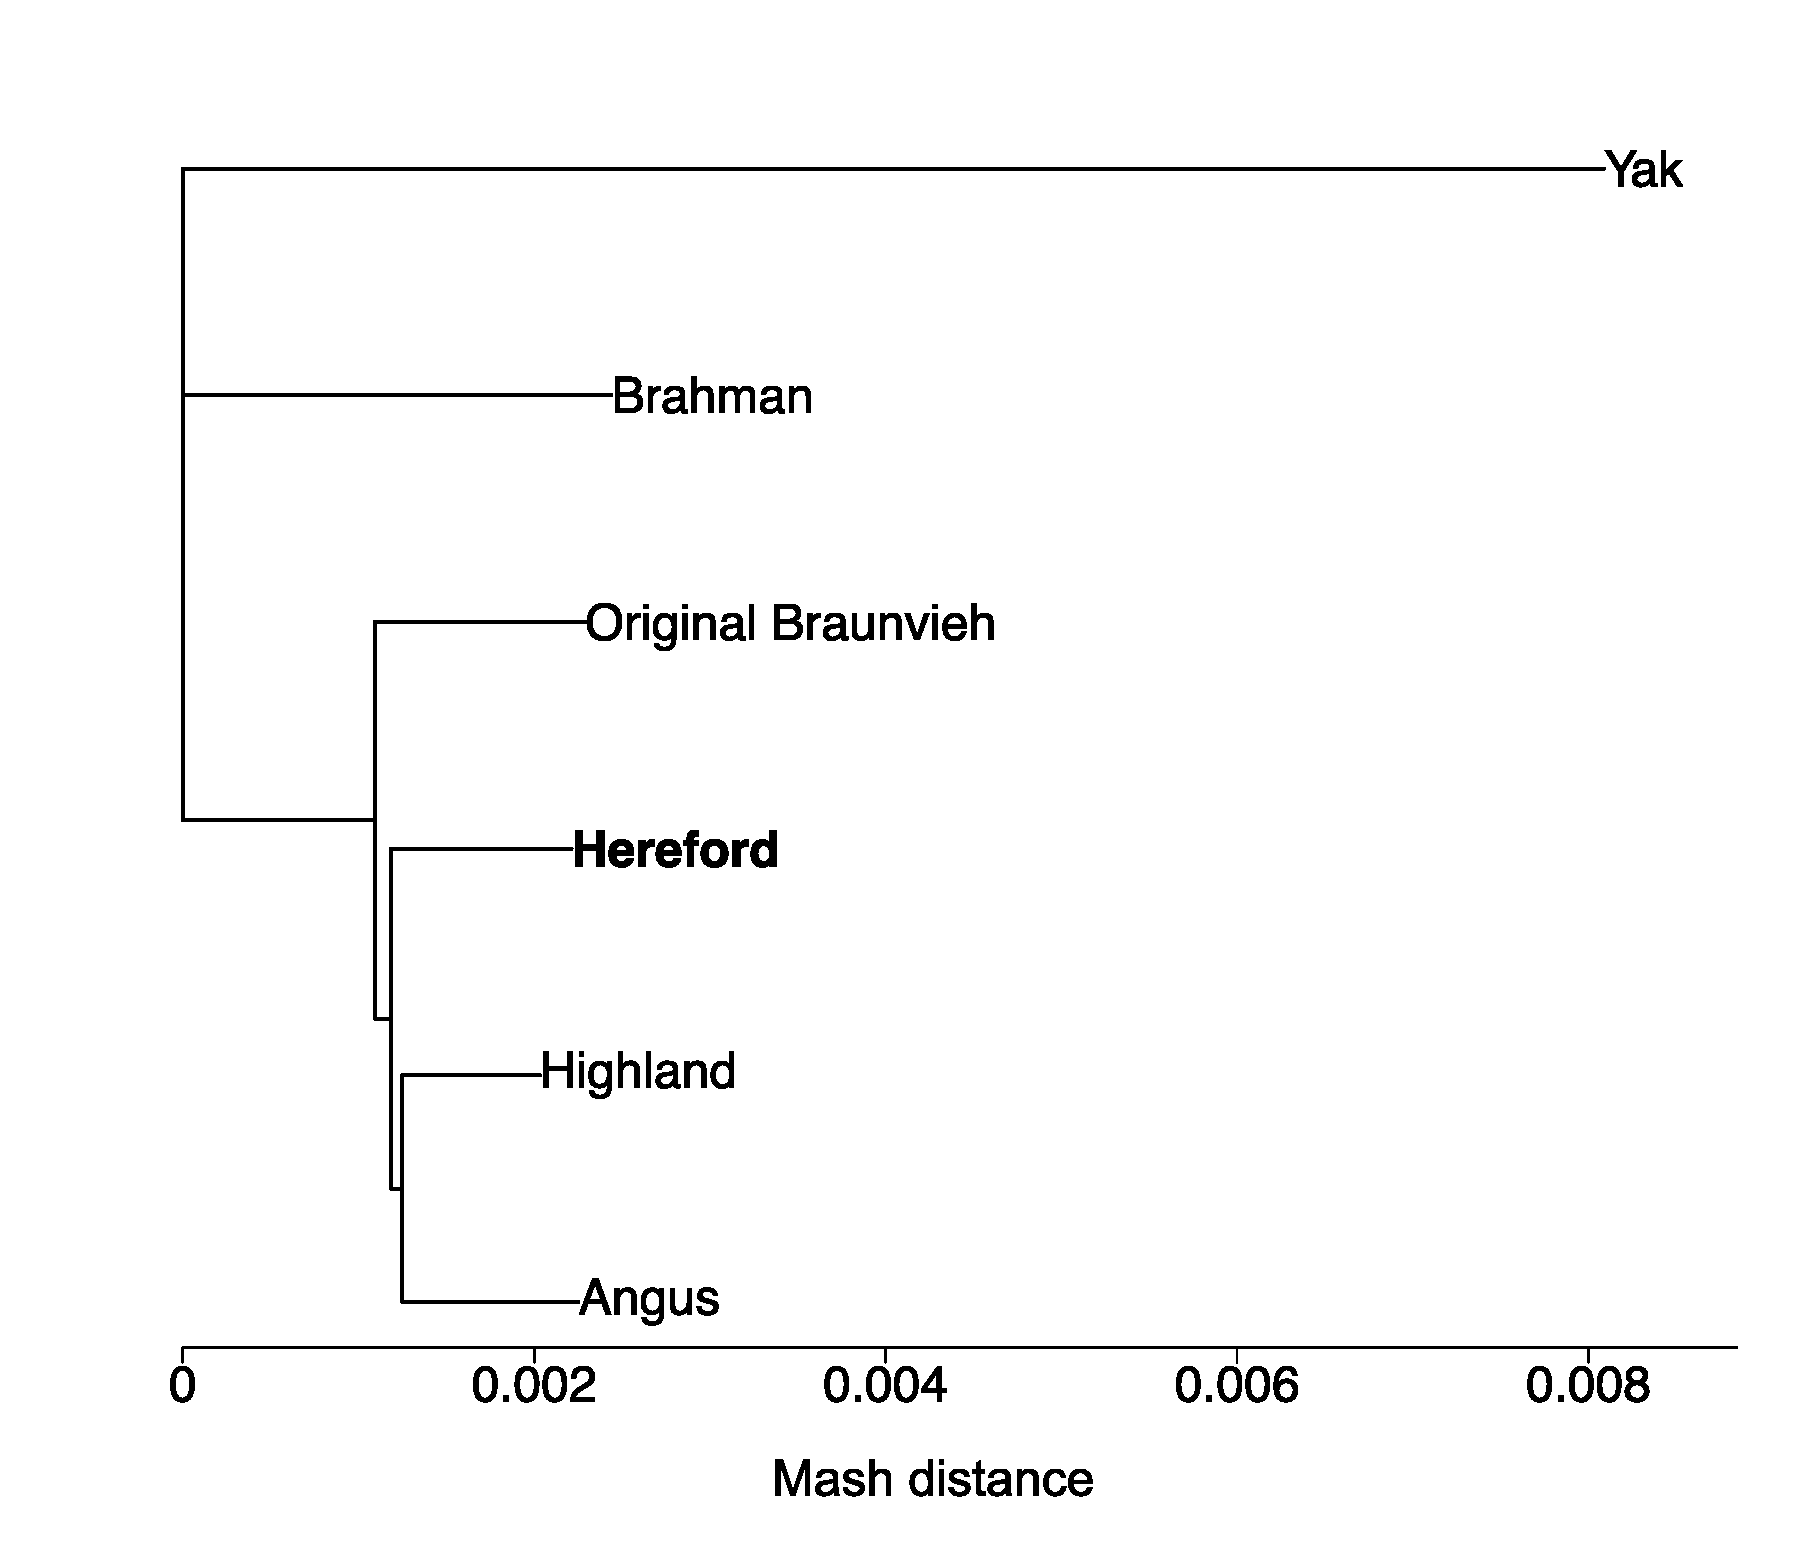
\includegraphics[width=\textwidth]{paper3/main_figure/Fig1.pdf}
        \caption[Phylogenetic distance between six genome assemblies]{\textbf{Phylogenetic distance between six genome assemblies.} \\
        \footnotesize{A Mash-based phylogenetic tree derived from six bovine assemblies, including the current Hereford-based \emph{Bos taurus} reference genome (\textbf{bold}). The yak assembly was used as the outgroup to root the tree during building.}}
        \label{fig41:phylo}
\end{figure}


The six assemblies were integrated into a multi-assembly graph with minigraph. We only considered autosomal sequences because the haplotype-resolved assemblies represent either paternal or maternal haplotypes, thus lacking either X or Y chromosomal sequences. The Hereford-based linear reference genome (ARS-UCD1.2) formed the backbone of the bovine multi-assembly graph. The graph was then augmented with the five additional assemblies, added in order of increasing Mash-distance from the ARS-UCD1.2 reference \citep{ondov2016mash} Fig. \ref{fig41:phylo}. Constructing this multi-assembly graph took 4.1 CPU hours and 58 GB of RAM, taking 36 minutes of wall-clock time when using 10 threads.

\subsection*{Recovery of non-reference sequences from the multi-assembly graph}

Our bovine multi-assembly graph represents 2,558,596,439 nucleotides, spread across 182,940 nodes connected by 258,396 edges. On average, a node spans 13,985 nucleotides and is connected by 1.4 edges. Of the edges, 141,086, 113,332, and 3,978 connect two reference nodes, a reference and non-reference node, or two non-reference nodes, respectively. 

The vast majority (2,489,385,779 or 97.29\%) of nucleotides in the multi-assembly graph originate from the linear reference backbone, covered in 123,483 nodes. These reference nodes span 23,088 bases on average, ranging from 100 to 1,398,882 bases. The incremental integration of the Highland, Angus, Original Braunvieh, Brahman, and yak assemblies added 8,847, 4,613, 3,555, 11,996, and 30,446 non-reference nodes, respectively containing 14,679,286, 5,537,769, 7,013,258, 11,116,220, and 30,864,
127 non-reference bases. The resulting multi-assembly graph contained 59,457 non-reference nodes spanning 69,210,660 bases. 

To determine the support of the non-reference nodes, we aligned individual assemblies back to the multi-assembly graph. Nodes were then labelled according to which assembly path traversed them (see \emph{SI Appendix}, Figs. \ref{sup_fig:s41} \& \ref{sup_fig:s42}). This approach enabled a straightforward confirmation of minigraph’s mapping accuracy. Only reference nodes should contain a Hereford label, since this assembly was used as the backbone of the graph. Mapping was highly accurate, as indicated by an F1 score of 99.97\%.

The non-reference nodes of the multi-assembly graph had a cumulative length of 43,341,418, 23,644,772, 18,202,102, 14,453,112 and 15,542,368 bases in the yak, Brahman, Original Braunvieh, Angus, and Highland assemblies. Yak and Brahman non-reference nodes were shorter on average compared to the taurine assemblies (\emph{SI Appendix}, Fig. \ref{sup_fig:s43}). Most non-reference nodes (41,855 or 70.40\%) and non-reference sequences (42.52 Mb, 69.52\%) were either private to yak (29,854 nodes, 29.9 Mb), Brahman (7,843 nodes, 8.22 Mb), or shared by both assemblies (4,158 nodes, 3.05 Mb). The Original Braunvieh, Highland, and Angus assemblies contributed 4.51, 2.78 and 2.39 Mb in 2,016, 1,938 and 1,759 nodes, respectively, that were not detected in any other assembly. The three taurine assemblies shared 668 nodes containing 0.77 Mb not detected in ARS-UCD1.2, yak, or Brahman. There were also 1,318 non-reference nodes with a cumulative length of 4.4 Mb supported by all five additional assemblies.

The core genome of the multi-assembly graph (i.e., nodes shared by all assemblies) is contained in 67,482 nodes with a cumulative length of 2,402,561,410 bases. About 6.10\% of the pangenome (115,458 nodes containing 156,035,029 bases) is flexible (i.e., not shared by all assemblies). Of the flexible part, 69,697 nodes containing 97,106,100 bases are shared by at least two assemblies, and 45,761 nodes with 58,928,929 bases are only found in one assembly. The profile of the multi-assembly graph changes markedly when distant assemblies (e.g., Brahman, yak) are added (\emph{SI Appendix}, \ref{sup_not:s42}).

The minigraph approach used to construct the multi-assembly graph does depend on an initial sequence forming a backbone. The choice of backbone consequently impacts the amount of non-reference sequence detected from each additional assembly (see \emph{SI Appendix}, \ref{sup_not:s43}). However, the overall effect on the sequence content of the multi-assembly graph is relatively minor, with 68.72±3.17 Mb of non-reference sequence identified across all possible backbones.

\subsection*{Structural variation discovery from the multi-assembly graph}

Using the bubble popping algorithm of gfatools \citep{li2020design}, we identified 68,328 structural variations present in the multi-assembly graph. To reveal true alleles within these structural variations, we traversed all possible paths through the bubbles (i.e., alleles) and retained only those that were supported by at least one assembly (\emph{SI Appendix}, Fig. \ref{sup_fig:s42}). Most of the structural variations had two alleles (64,224 or 94\%). The remaining 4,104 structural variations were multi-allelic, most of which had three alleles (3,324 or 81\%). We identified 141,747 alleles at the structural variations, including 73,506 non-reference alleles with a cumulative length of 74,453,929 bases.  

We overlapped the breakpoints of the structural variations with the Ensembl annotation (build 101) of ARS-UCD1.2. Almost all structural variations were either intergenic (47,642 or 69.81\%) or intronic (20,227 or 29.64\%). There were 170 and 202 exons and coding sequences, respectively, of 338 unique genes affected by structural variations. A Panther GO-Slim Biological Process \citep{mi2019panther} analysis indicated that these genes are enriched for genes related to the adaptive immune response (4.35$-$fold, $P=0.04$), T-cell mediated immunity (6.37$-$fold, $P=0.04$), actin filament depolymerization (8.54$-$fold, $P=6.56x10^{-3}$), microtubule cytoskeleton organization (10.48$-$fold, $P=1.85x10^{-4}$), and iron-sulfur cluster assembly (9.96$-$fold, $P=0.02$). 

The non-reference alleles consisted of 40,369 insertions and 33,137 deletions with an average length of 1,181 and 1,210 bases respectively (\emph{SI Appendix}, Table \ref{sup_tab:s41}). The cumulative length (absolute difference between reference and non-reference allele) was longer for insertions (47,691,942 bases) than deletions (40,101,303 bases). This pattern was similar for biallelic variations (35,748 and 28,476 biallelic insertions and deletions, respectively, encompassing 37,388,222 and 28,373,582 bases with an average variant length of 1,045 and 996 bases). The multi-assembly graph contained more complete insertions (20,432; i.e., only non-reference sequences present in the bubbles, thus reference length is 0) than alternate insertions (15,316; i.e., both reference and non-reference sequences present but non-reference allele is longer). The pattern was similar for deletions. The multi-allelic structural variations had 13,299 alleles including 9,282 non-reference alleles with 4,621 insertions and 4,661 deletions, respectively, affecting 11,727,721 and 10,303,720 bases. Bubbles with multi-allelic structural variations contained more mixed mutations (1,941; both deletions and insertions detected within the same bubble) than multiple mutations of the same type (994 and 1,082 for multiple insertions and deletions, respectively). 

When compared to the ARS-UCD1.2 backbone, the yak, Brahman, Original Braunvieh, Angus, and Highland assemblies contained respectively 49,836, 22,976, 10,965, 10,735, and 10,560 non-reference alleles (Fig. \ref{fig42:nrfsec}). Most non-reference alleles (36,443, total length: 30 Mb) were private to the yak assembly. We detected 9,267, 2,232, 2,133, and 2,037 non-reference alleles, respectively, containing 10.1, 4.9, 3.8, and 3.3 Mb that were private to the Brahman, Original Braunvieh, Highland, and Angus assembly (Fig. \ref{fig42:nrfsec}, \emph{SI Appendix}, Fig. \ref{sup_fig:s45}). We also found 1,749 alleles within the 4.4 Mb of non-reference sequence (2.1 Mb of which is non-repetitive) shared by all assemblies except ARS-UCD1.2.

We mapped PacBio HiFi reads from a Nellore (\emph{Bos taurus indicus}) x Brown Swiss (\emph{Bos taurus taurus}) crossbred bull to the multi-assembly graph to examine support for the non-reference alleles. Nearly one third of the structural variation breakpoints had support from the hybrid cattle, while this rose to approximately three-quarters after excluding nodes with only yak labels. Since neither parental breed is present in the multi-assembly graph, this suggests that the discovered structural variation may be prevalent in different breeds of taurine and indicine cattle. 

\begin{landscape}
    \begin{figure}[!htb]
        \centering
        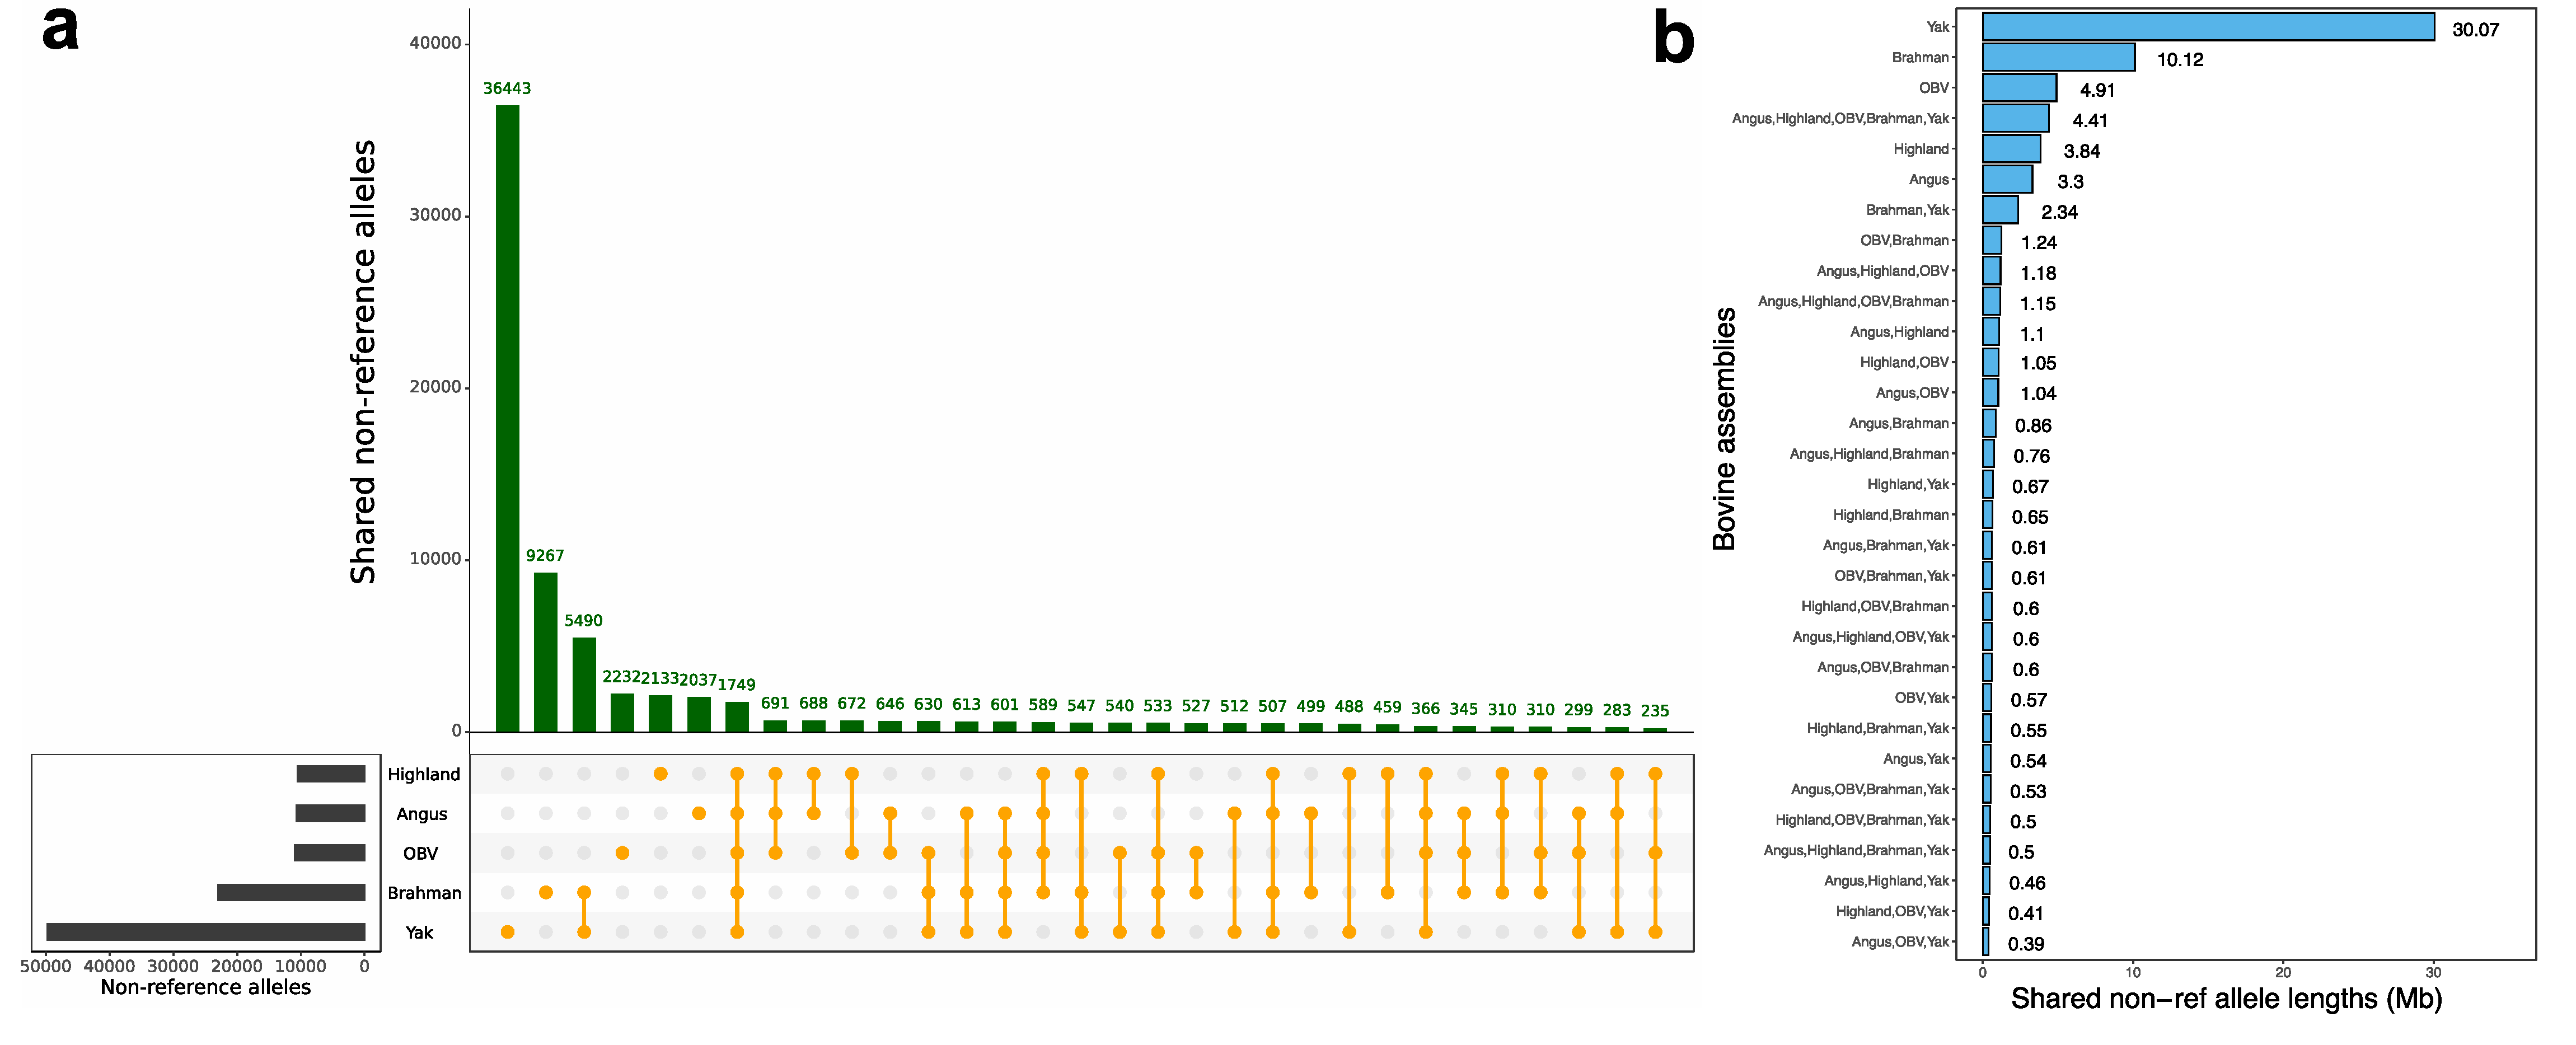
\includegraphics[width=1.5\textwidth]{paper3/main_figure/Fig2.pdf}
            \caption[Non-reference alleles detected across assemblies]{\textbf{Non-reference alleles detected across assemblies.} \\
            \footnotesize{Intersection of non-reference alleles \textbf{(a)} and cumulative length of the alleles \textbf{(b)} found in five assemblies when compared to ARS-UCD1.2. OBV : Original Braunvieh.}}
            \label{fig42:nrfsec}
    \end{figure}  
\end{landscape}


\subsection*{Sequence content of the structural variations}

In order to investigate the functional relevance of the non-reference sequences, we extracted 45,357 non-reference alleles from the 70,329,827 non-reference bases in the multi-assembly graph (\emph{SI Appendix}, Fig. \ref{sup_fig:s46}). These sequences originate from 38,906 biallelic and 6,451 multiallelic structural variations, respectively, that have a cumulative length of 43,003,591 and 27,326,236 bases. On average, the alleles of multiallelic structural variations were four times longer than that of biallelic bubbles (4,205 versus 1,104 bases). 
 
The non-reference sequences are largely comprised of repetitive elements (53,690,260 bases or 76.34\%, \emph{SI Appendix}, Fig. \ref{sup_fig:s47}). LINE/L1 and LINE/RTE-BovB account for 28.04 (52.22\%) and 6.77 (12.61\%) Mb repetitive non-reference bases, respectively. Repetitive sequences (both interspersed and simple repeats) are more evenly distributed across the autosomes than non-repetitive sequences. Both repetitive and non-repetitive non-reference sequences were detected at two regions on bovine chromosomes 18 and 23 that encompass the leukocyte receptor complex and the major histocompatibility complex (\emph{SI Appendix}, Fig. \ref{sup_fig:s48}). 

We hypothesized that the 16,639,567 non-repetitive non-reference bases contain transcribed sequences. A BLASTX search of these sequences against a protein sequence database of Bos and related species revealed hits for 403 structural variations containing 299,337 non-reference bases. As a complementary approach, we predicted genes from the non-repetitive sequences using the Augustus software tool. The \emph{ab initio} prediction revealed 857 gene models from 768 distinct structural variations that had a minimum coding sequence length of 150 bp, including 374 complete gene models with transcription start site, start codon, exons, stop codon, and transcription termination site (\emph{SI Appendix}, Table \ref{sup_tab:s42}). On average, the transcript, coding sequence, and protein length of the complete gene models is respectively 4,742 bp, 794 bp, and 264 amino acids. 

\subsection*{\emph{De novo} transcript assembly from the non-reference sequences}

As the two complementary gene prediction methods indicated that these non-reference sequences contain transcribed features, we sought experimental evidence. We appended the 70 Mb of repeat masked non-reference sequences contained in 45,357 additional contigs to the ARS-UCD1.2 reference, making an extended reference genome. This renders the non-reference sequences amenable to current methods of linear mapping of transcriptome data. Using HISAT2, we aligned liver transcriptomes from 39 cattle across taurine (Angus, Holstein, Jersey) and indicine (Brahman) breeds to both the linear reference as well as the extended reference. We also aligned transcriptomes from Dominette, the animal sequenced to assemble the \emph{Bos taurus} reference genome. A greater portion of reads mapped to the extended reference compared to the original reference for all examined samples (\emph{SI Appendix}, Fig. \ref{sup_fig:s49}). Across the 40 samples, the overall mapping rate increased by 0.037\%, which corresponds to approximately $\sim$18,000 reads for a paired-end RNA-seq dataset of 25 million reads. The mapping improvements were larger for samples with greater genetic distance from the reference genome. Brahman had the largest improvement (0.060\%), followed by the taurine breeds: Angus (0.032\%), Holstein (0.026\%), and Jersey (0.030\%). As expected, Dominette benefitted the least (0.010\%), but still demonstrated an improvement over using the original reference. 

Next, we used StringTie2 \citep{kovaka2019transcriptome}, guided with gene models predicted by Augustus (see above), to assemble reads which aligned to non-reference sequences into 1,431 non-reference genes. Of these, 885 were expressed at TPM ≥ 1 in at least one breed, including 405 that were originally predicted by Augustus. We selected these 405 putative genes, supported by both \emph{ab initio} prediction and \emph{de novo} transcript assembly for further analyses. 

Only 263 of the 405 putative genes were expressed at TPM ≥ 1 in Dominette, with BLASTP queries indicating they may mostly be divergent copies of ribosomal proteins or olfactory receptors. The remaining 142 genes were expressed at TPM ≥ 1 in Angus, Holstein, Jersey or Brahman cattle. Most were expressed in Brahman cattle (Fig. \ref{fig43:rnanov}a), including 20 genes specific to this indicine breed. Among the taurine breeds, Angus contributed more genes than either Holstein or Jersey cattle. Approximately half of these genes, 68 of the 142, were common to all four nonreference breeds (Fig. \ref{fig43:rnanov}b). The average expression was significantly higher ($P=0.004$, one-tailed t-test) for genes that were expressed in at least two breeds (N=106, TPM=13.48) than genes expressed in only one breed (N=36, TPM=1.64). BLASTP queries provided additional support for 57 out of 142 non-reference genes (\emph{SI Appendix}, Fig. \ref{sup_fig:s410}). The top hits suggest that these genes encode proteins related to: immune response (antigen-presenting glycoprotein, immunoglobulin, BOLA (Bovine Leukocyte Antigen), killer-T-cell, interferon, Ig-like lectin, CMRF35, MHC (Major Histocompatibility complex), cytokine), signalling (G-protein signalling protein, tyrosine-phosphatase), cytoskeleton regulations (myosin, actin, twinfilin, KANTB1), lipid metabolism (apolipoprotein, lipid-binding protein), and protein modifications (heat-shock chaperone, ubiquitin conjugating enzyme, rhoA ubiquitin). 



\begin{figure}[!htb]
    \centering
    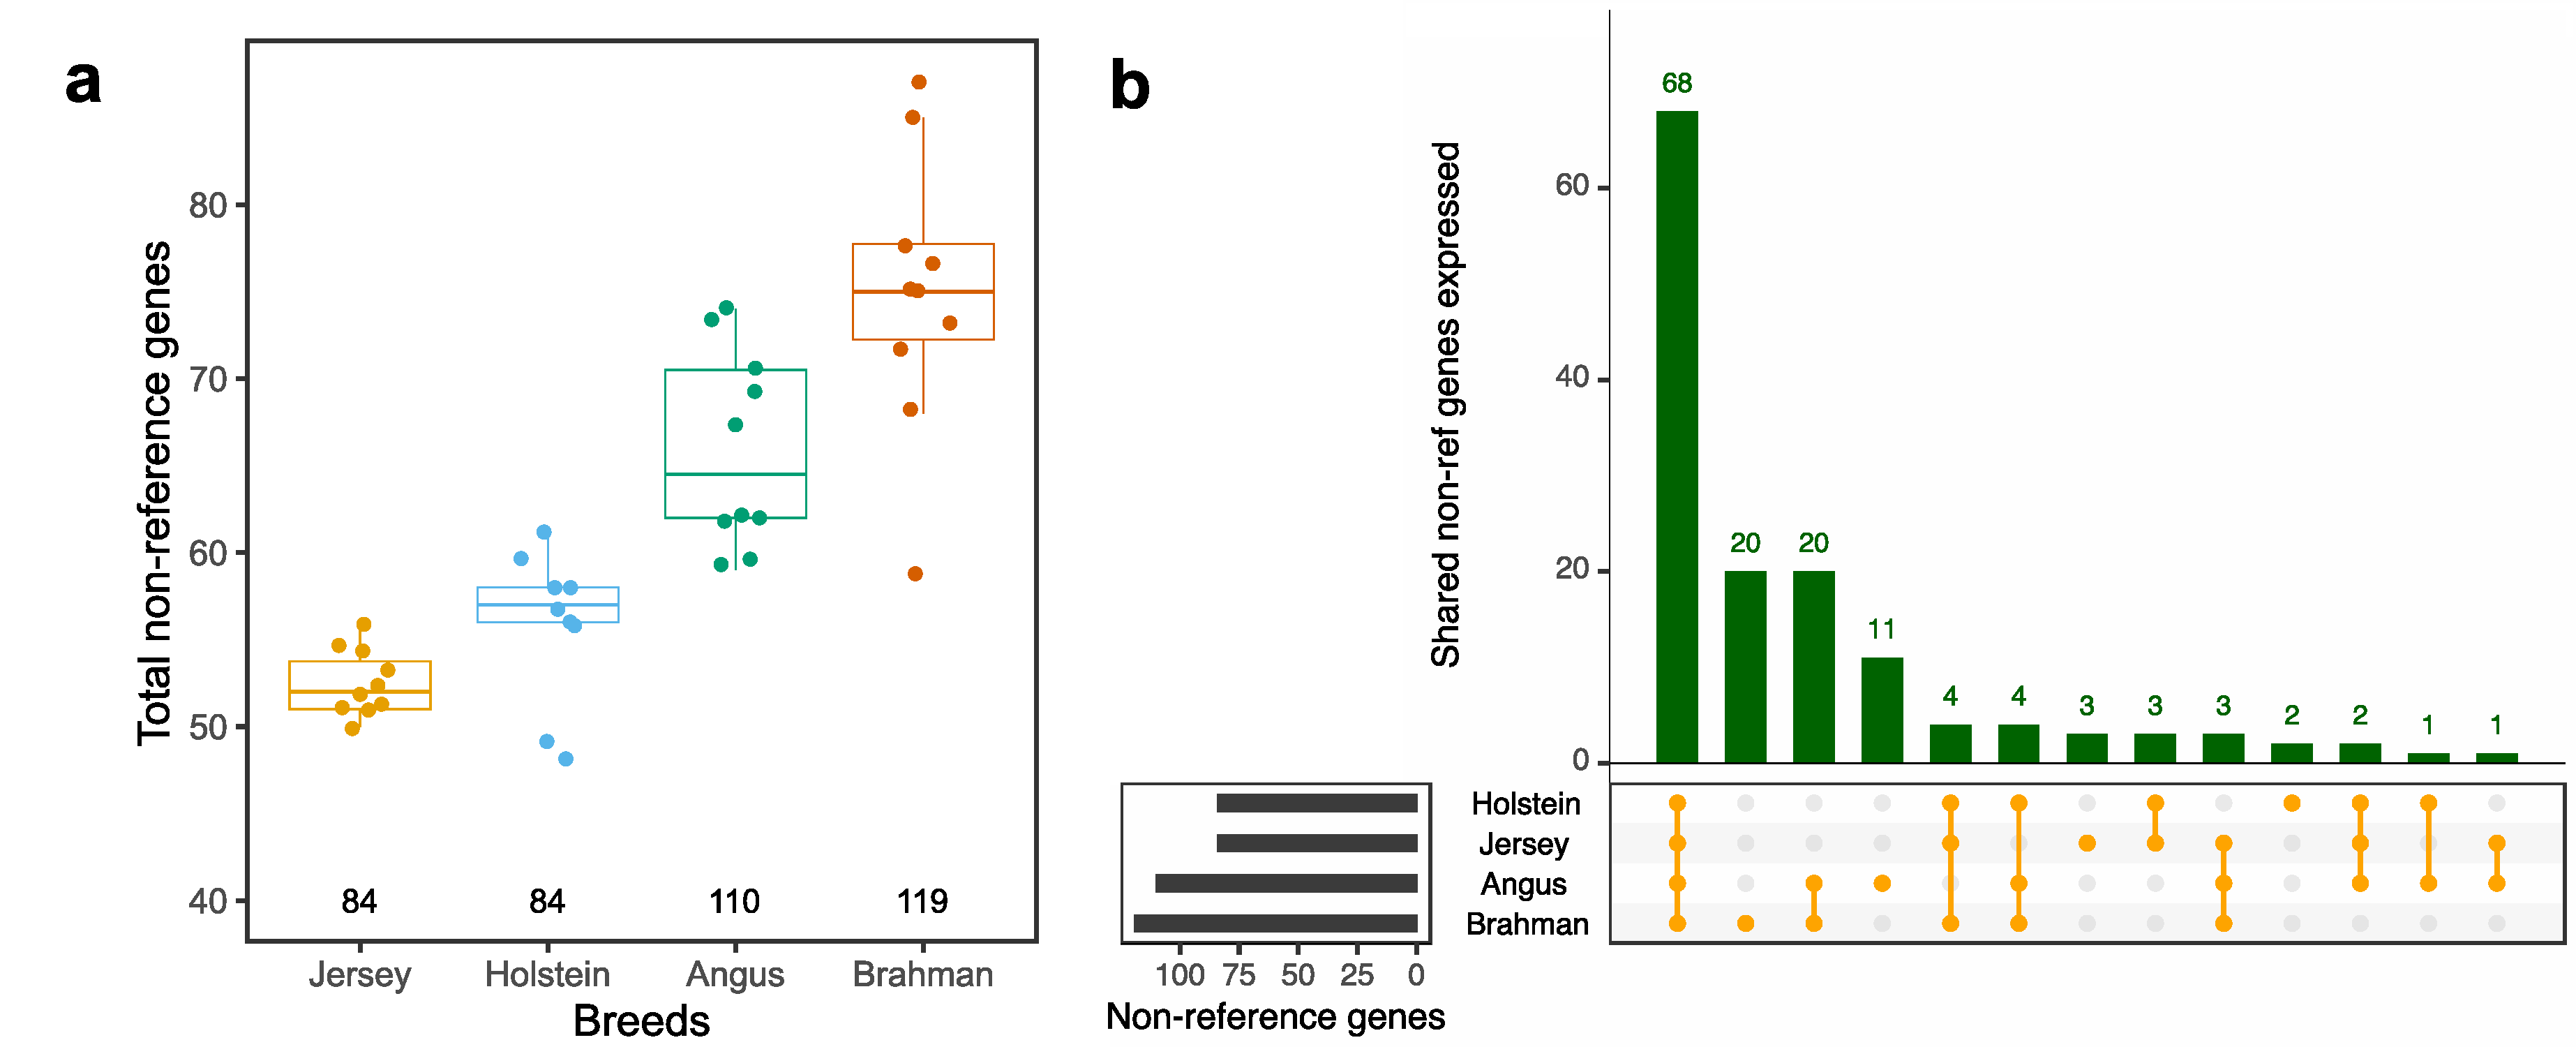
\includegraphics[width=\textwidth]{paper3/main_figure/Fig3.pdf}
        \caption[Transcribed genes detected from non-reference sequences]{\textbf{Transcribed genes detected from non-reference sequences.} \\
        \footnotesize{\textbf{(a)} Number of non-reference genes expressed ≥1 TPM in liver tissue from taurine (Jersey, Holstein, Angus) and indicine (Brahman) cattle breeds. Each point represents the number of non-reference genes detected per animal. The number of distinct non-reference genes detected for each breed is indicated below the boxplots. \textbf{(b)} Expression of 142 non-reference genes in the four cattle breeds.}}
        \label{fig43:rnanov}
\end{figure}

\subsection*{Non-reference sequences contain differentially expressed genes}

To investigate if the non-repetitive sequences also encode transcripts that are differentially expressed between individual \emph{Bos taurus} cattle, we obtained publicly available peripheral blood leukocyte transcriptome data for eight \emph{Mycobacterium} bovis-infected and eight non-infected Holstein cattle \citep{mcloughlin2014rna}. Following the transcriptome analysis introduced earlier, the RNA sequencing reads were aligned to both the standard and extended ARS-UCD1.2 reference genome sequence. Between 8,616,414 and 23,940,699 RNA sequencing reads aligned to the standard and between 8,631,277 and 23,977,859 RNA sequencing reads aligned to the extended reference genome. The subsequent \emph{de novo} transcript assembly from the non-reference sequences produced 949 transcripts, encoded by 661 non-reference genes. We appended them to the Ensembl ARS-UCD1.2 annotation, yielding a total of 28,268 genes. Considering only unique alignments, we detected expression levels $≥$ 1 counts per million in at least eight samples for 13,085 genes, including 272 non-reference genes. We subsequently tested these genes for differential expression, finding 3,646 genes, including 36 non-reference genes, which were differentially expressed (FDR ≤ 0.05) between \emph{Mycobacterium bovis}-infected and non-infected cattle (Fig. \ref{fig44:rnadif}a). The top differentially expressed genes from our extended Ensembl ARS-UCD1.2 annotation, as well as their transcript abundances in cases and controls, agreed well with the original findings from \citet{mcloughlin2014rna} that were based on the previous UMD3.1 annotation (Pearson R log$_2$ fold-change: 0.99) as well as with those from the standard ARS-UCD1.2 reference genome annotation (Pearson R log$_2$ fold-change: 0.99, \emph{SI Appendix}, \ref{sup_not:s44}). 


Within the 36 differentially expressed non-reference genes, 28 and 8 are respectively up- and downregulated in peripheral blood leukocytes of \emph{Mycobacterium bovis}-infected cattle, with an average 2-fold change compared to non-infected controls (\emph{SI Appendix}, Fig. \ref{sup_fig:s411}). Multidimensional scaling representations of transcript abundance estimates of the 36 differentially expressed genes separated \emph{Mycobacterium bovis}-infected from non-infected cattle (Fig. \ref{fig44:rnadif}b). BLASTX queries against a protein reference database provided additional support for 13 out of 36 differentially expressed genes (\emph{SI Appendix}, Table \ref{sup_tab:s43}). The top upregulated non-reference gene supported by the BLASTX query (4.04-fold increase, $P=1.98x10^5$) encodes the Workshop Cluster (WC) 1.1-like protein, i.e., a receptor expressed on gamma delta T cells that modulates the immune response to \emph{Mycobacterium bovis} infections \citep{mcgill2014specific,damani2018variegated,kennedy2002modulation}. 

The top downregulated non-reference gene supported by the BLASTX query encodes a protein with high similarity (79.80\%) to leukocyte immunoglobulin-like receptor A5 (LILRA5). LILRA5 triggers the strength of the innate immune response to \emph{Mycobacterium} infections \citep{bah2018meta} and might serve as a target for pathogen-mediated immunomodulation. Many genes of the leukocyte receptor complex are missing in the assembled chromosomes of the ARS-UCD1.2 reference \citep{bakshy2021development}; instead, LILRA5 (LOC100139766) is annotated on a 236 kb long unplaced scaffold (NW\_020190675). A non-reference gene encoding a protein similar to LILRA5 is located within a 20.4 kb insertion of the multi-assembly graph at 62,471,732 bp on chromosome 18. Both taurine (Original Braunvieh) and indicine (Brahman) assemblies support this insertion. The gene encoding LILRA5 is expressed at 9.59$±$2.54 and 23.10$±$8.30 CPM, respectively, in \emph{Mycobacterium bovis}-infected and non-infected cattle, corresponding to a 2.19$-$fold decrease ($P=10^{-4}$) in infected cattle (\emph{SI Appendix}, Table \ref{sup_tab:s43}).

\begin{figure}[!htb]
    \centering
    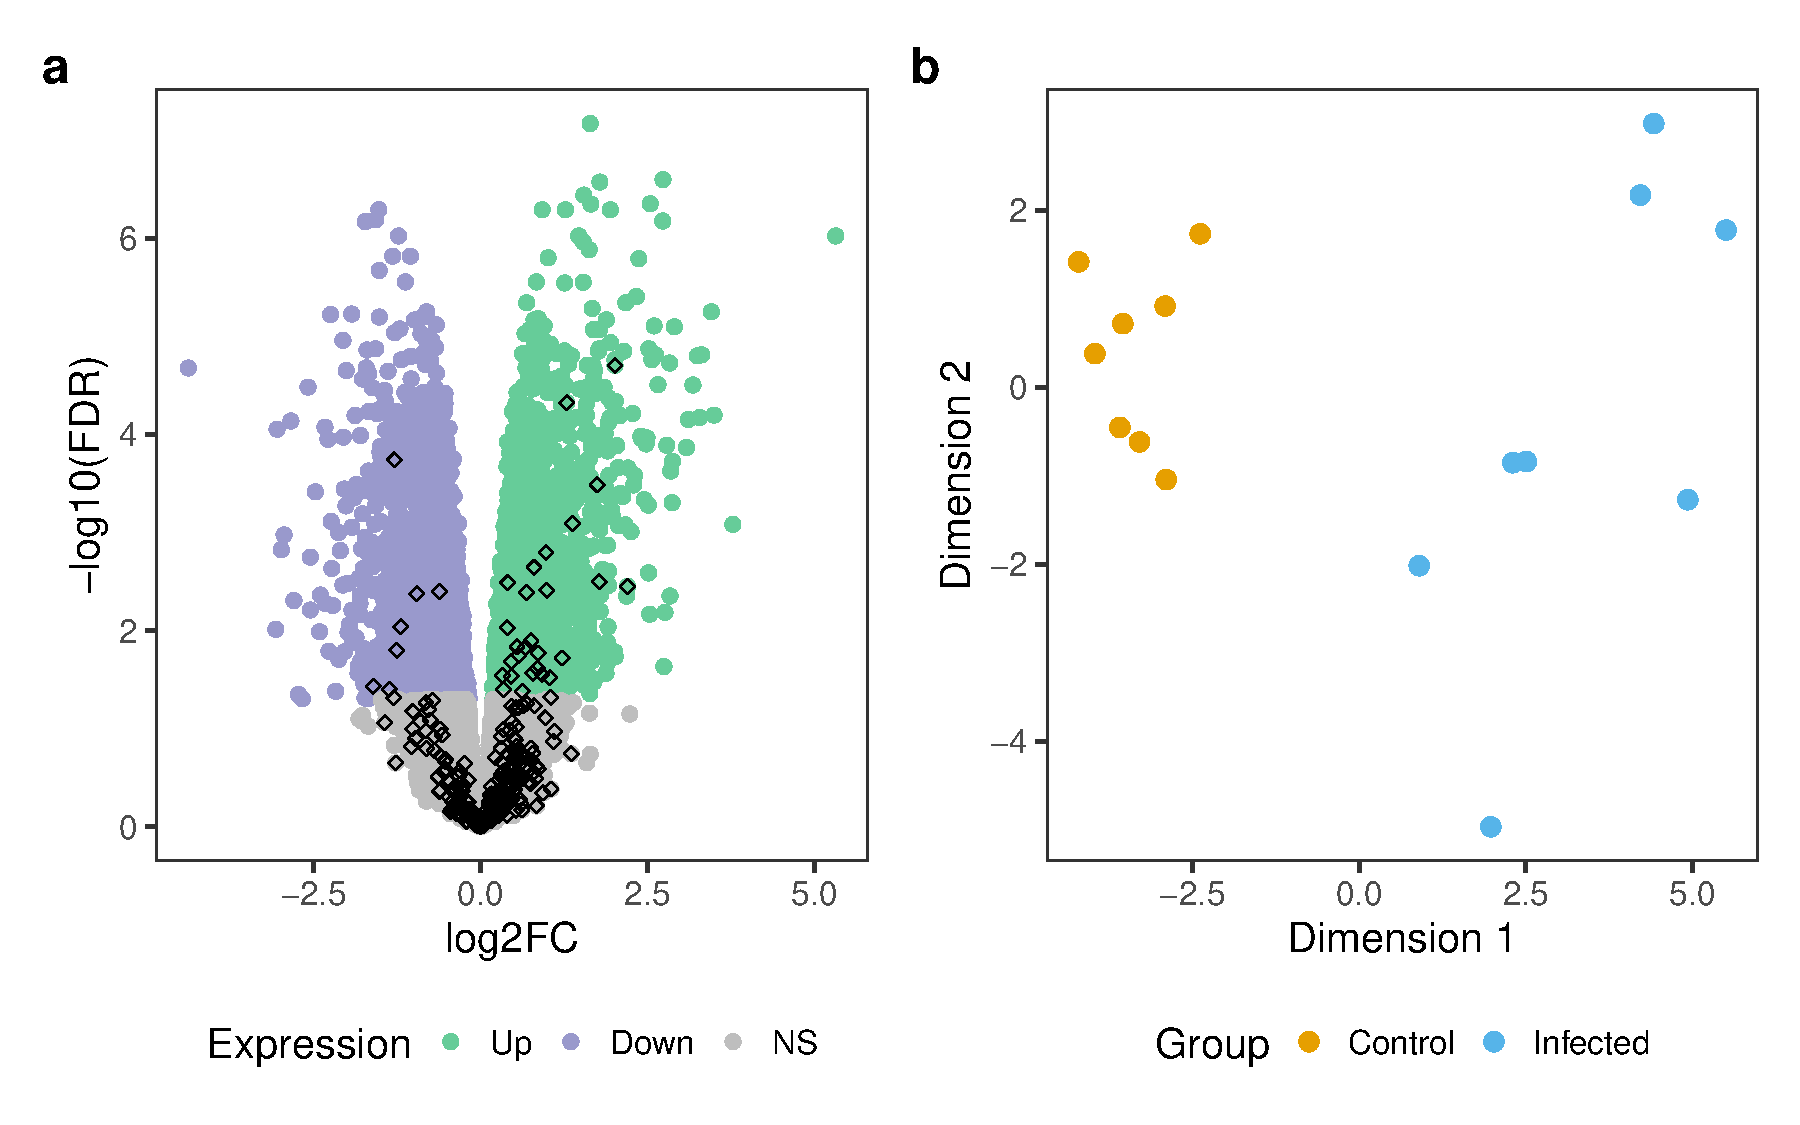
\includegraphics[width=\textwidth]{paper3/main_figure/Fig4.pdf}
        \caption[Differential expression non-reference genes]{\textbf{Differentially expressed non-reference genes.} \\
        \footnotesize{\textbf{(a)} Volcano plot representing results from the differential expression analysis. Green and purple color indicates genes that are up- and downregulated (FDR ≤ 0.05), respectively, in peripheral blood leukocytes of \emph{Mycobacterium bovis}-infected cattle. Diamond shapes indicate the 272 genes found in non-reference sequences. \textbf{(b)} Multidimensional scaling plot of 36 differentially expressed non-reference genes in \emph{Mycobacterium bovis}-infected (blue) and non-infected (orange) Holstein cattle.}}
        \label{fig44:rnadif}
\end{figure}


\subsection*{Variant discovery from the non-reference sequences}

Next, we mapped short sequencing reads, with an average of 19-fold sequencing coverage, from 45 cattle representing five taurine breeds against ARS-UCD1.2 and the extended ARS-UCD1.2 reference genome. An average number of 34,342 reads per sample mapped perfectly within 50 bp of the breakpoints of the newly added contigs indicating that the addition of 100 bp flanking sequence was sufficient to facilitate accurate alignments. Across 45 samples, the average mapping rate increased by 0.0176\% over ARS-UCD1.2, corresponding to approximately $\sim$100,000 sequencing reads for a DNA sample sequenced at 30-fold coverage. The mapping rate increased more noticeably for Brown Swiss (0.024\%) and Original Braunvieh (0.021\%) than Holstein (0.015\%) and Simmental (0.016\%) cattle (\emph{SI Appendix}, Fig. \ref{sup_fig:s412}). Similarly, to the transcriptome mapping, sequence reads from Dominette benefitted the least from the extended reference genome (0.006\%). However, the increase in mapping rate was greater (0.013\%) for other Hereford cattle. For all breeds, the extended reference genome also enabled more perfect alignments (alignments without difference from the reference), less partially mapped (i.e., clipped) reads, and less reads with supplementary alignments. However, the proportion of reads with unique alignment was lower for the extended than standard reference genome (\emph{SI Appendix}, Table \ref{sup_tab:s44}). 

We next investigated the alignments against the 2,115,702 non-repetitive non-reference bases detected in all assemblies except ARS-UCD1.2. Among these, 919,761 bases were covered by confident alignments (≥10-fold) from Dominette. This suggests that, although absent from the autosomal assembly, these sequences do occur in the animal used to construct the reference. However, 1,195,941 bp were not covered with reads from Dominette, but instead from Brown Swiss, Holstein, Original Braunvieh or Simmental samples. Strikingly, reads from non-Dominette Hereford samples covered 745,392 of the 1,195,941 bases. This directly implies that Dominette has individual-specific deletions, which are either rare or absent in other Hereford cattle.

Mapping against the extended reference resulted in many reads changing alignment location to the non-reference additions. Most (85.55\%) of the reads mapping at non-reference sequences already mapped to the original ARS-UCD1.2 reference genome, although 5\% of these mapped to unplaced contigs, while 14.45\% were previously unmapped. These mappings displayed an increase in the average mapping quality (22 to 44), alignment score (110 to 142), and alignment identity (0.975 to 0.995). The proportion of clipped reads decreased from 39\% to 4\%. The subset of these reads which were previously unmapped showed even greater improvements (\emph{SI Appendix}, Fig. \ref{sup_fig:s413}).

Using reads with mapping quality greater than 10 for reference-guided sequence variant genotyping yielded 83,250 filtered variants (73,709 SNPs, 9,541 Indels) in non-reference sequences that were identified by both SAMtools and GATK. These variants formed 80,995 biallelic and 2,255 multi-allelic sites, with a Ti:Tv (Transition:Transversion) ratio of 1.91, averaging 1.18 variants per kb. 3890 small variations (Ti:Tv ratio: 1.79) were detected within 50 bp of the breakpoints of the newly added contigs. On average each Brown Swiss, Original Braunvieh, Holstein, Simmental, and Hereford animal respectively had 31,028, 29,685, 29,851, 30,309, and 15,845 variant sites in non-reference bases (Fig. \ref{fig45:varnrf}a). A DNA sample from Dominette had considerably fewer polymorphic sites at non-reference bases, only 7,531. Most variants (32.67\%) had alternate allele frequency less than 0.1, and 193 were fixed for the alternate allele (\emph{SI Appendix}, Fig. \ref{sup_fig:s414}). The top principal components from a genomic relationship matrix that was built from the 83,250 non-reference variants separated the animals by breeds (Fig. \ref{fig45:varnrf}b,c). Functional annotation based on the gene models predicted from Augustus indicated that most non-reference variants were either intergenic (83\%) or intronic (7.5\%). 1138 variants (Ti:Tv ratio: 1.83) were in putative coding sequences, of which 54 were classified as "HIGH IMPACT” variants (\emph{SI Appendix}, Table \ref{sup_tab:s45}).


\begin{figure}[!htb]
    \centering
    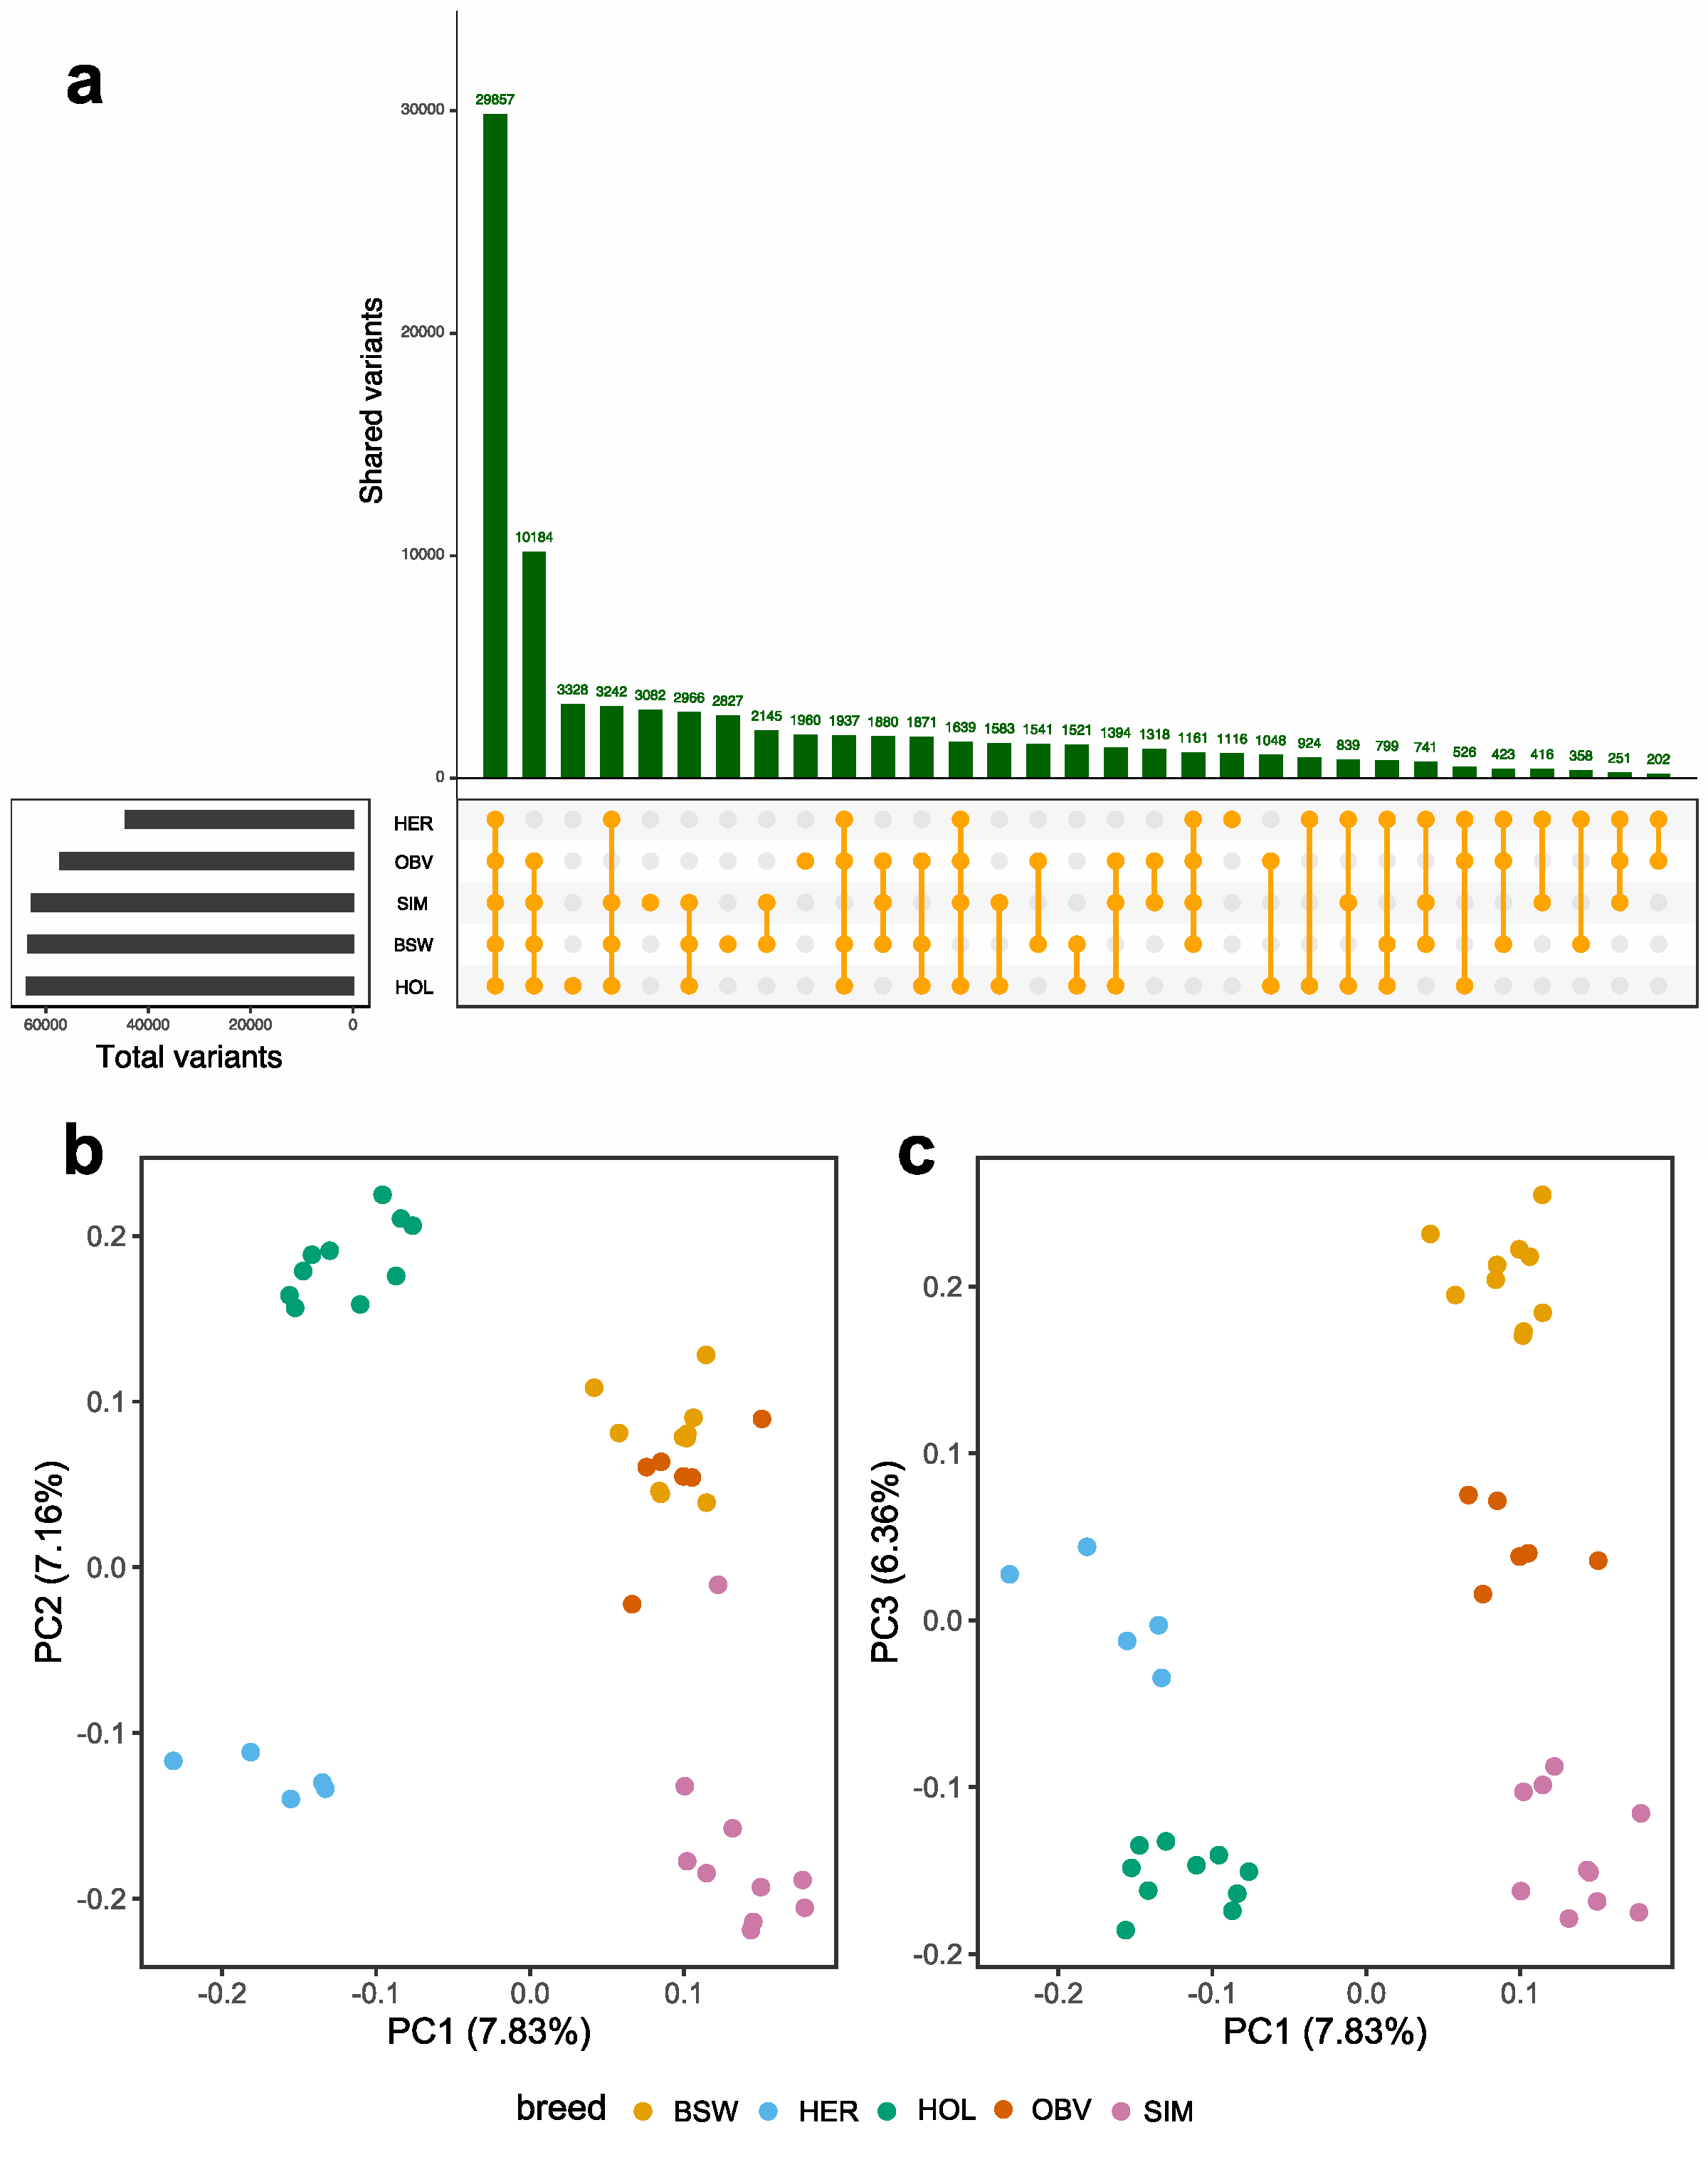
\includegraphics[width=0.8\textwidth]{paper3/main_figure/Fig5.pdf}
        \caption[Polymorphic sites detected from non-reference sequences in five breeds]{\textbf{Polymorphic sites detected from non-reference sequences in five breeds.} \\
        \footnotesize{\textbf{(a)} Sharing of 83,250 variants across five taurine cattle breeds (BSW: Brown Swiss, HER: Hereford, HOL: Holstein, OBV: Original Braunvieh, SIM: Simmental). \textbf{(b, c)} The top three principal components (PC) of a genomic relationship matrix constructed from non-reference sequence variants separate the animals by breed.}}
        \label{fig45:varnrf}
\end{figure}


\section{Discussion}

We utilize a bovine multi-assembly graph to uncover sequences that are not included in the Bos taurus reference genome. Novel contigs can also be assembled from unmapped reads, but placing them onto reference coordinates is difficult \citep{sherman2019assembly,golicz2016pangenome}. Our approach provides physical coordinates for the novel sequences because the breakpoints anchor them onto the reference genome. Despite including the genetically distant yak, constructing the multi-assembly graph using minigraph \citep{li2020design} was computationally efficient and scalable. Our multi-assembly graph utilizes a well-annotated backbone assembly to identify non-reference sequences from other assemblies. We show that the choice of the backbone as well as its genetic distance to all other assemblies influences the amount of non-reference bases uncovered through the multi-assembly graph. Sophisticated algorithms facilitate the reference-free alignment of thousands of assemblies \citep{armstrong2020progressive}. To determine the origin of the non-reference sequences, we developed an approach to assign labels to all nodes in the multi-assembly graph. Our evaluation showed that this strategy is highly accurate.

By systematically characterizing structural variations in multiple assemblies from domestic cattle and their close relatives, we detect 45,357 autosomal segments with a cumulative length of 70,329,827 bases that are not part of \emph{Bos taurus} reference genome. To obtain continuous non-reference sequences spanning multiple non-reference nodes, we recovered the non-reference alleles from structural variations. The number of bases detected in our study that are not in the \emph{Bos taurus }reference genome is comparable to values reported for pigs (72.5 Mb) \citep{tian2019building} and goats (38.3 Mb) \citep{li2019towards}, based on multi-assembly graphs constructed from 11 and 8 animals representing different breeds respectively. In our study, many non-reference sequences originate from yak. Hybridizing between yak and cattle is widely practiced, and results in fertile female descendants. However, multiple generations of backcrossing are required for males to resume fertility \citep{qi2010assessment}. A pangenome constructed from domestic cattle and their extant relatives as recently proposed by the Bovine Pangenome Consortium \citep{smith2020genome} will reveal variants that were lost during domestication and the separation of cattle into specialized breeds \citep{khan2020super}. For instance, some of the 8 million non-reference bases specific to Brahman might contribute to the adaptation of indicine cattle to harsh environments. Individual taurine assemblies also contain between 14 and 18 million bases that are missing in the Hereford-based reference assembly, many of which are shared between individuals. This value is somewhat higher than the 5-10 million non-reference bases detected per human genome \citep{ameur2018novo,audano2019characterizing,duan2019hupan}, possibly because cattle breeds have diverged more strongly than human populations due to intense artificial selection. Each of the three taurine assemblies contains approximately 3 million autosomal non-reference bases that were not detected in any other assembly. There were also 4.4 million non-reference bases, of which 2.1 million were non-repetitive, that were present in all assemblies except the reference. This includes 1.2 million bases that are either specifically deleted in the Hereford breed or the animal used to build the reference, inadvertently propagating reference-bias.

A reference graph may integrate linear reference coordinates, non-reference sequences, and shorter variants \citep{hickey2020genotyping}. However, as many genome analysis tools still rely on a linear coordinate system, we append the non-reference sequences linearly to the ARS-UCD1.2 reference genome. Adding 100 bp flanking sequence on either side of the breakpoints facilitated accurate alignment of sequencing reads at the boundaries of the novel contigs. A graph-based approach might enable the mapping of sequencing reads spanning breakpoints \citep{hickey2020genotyping}. We considered only variations larger than 100 bp because integrating smaller variations increases the complexity of the resulting reference with limited benefit for downstream analyses \citep{li2020design}. We show that our extended ARS-UCD1.2 reference genome leads to improved DNA and RNA sequence read mapping in indicine and taurine cattle, even for breeds that did not contribute to the multi-assembly graph. However, excessively adding novel sequences to the reference genome carries the risk of increasing the number of ambiguous alignments.

The non-reference sequences comprise more repetitive elements than the overall ARS-UCD1.2 reference genome (76\% versus 48\%), but less than non-reference insertions detected from human pangenomes (88\%) \citep{sherman2019assembly,ameur2018novo}. Many non-reference sequences with repetitive elements were observed at immune gene complex loci, corroborating that these regions are highly repetitive \citep{schwartz2017evolution}. The immune gene complex loci also contain many non-repetitive non-reference sequences suggesting great allelic diversity which may cause assembly problems \citep{bakshy2021development}, thus resulting in gaps and missing sequences in the primary ARS-UCD1.2 assembly. 


We show that the 16.6 million non-repetitive non-reference bases encompass transcribed features. An \emph{ab initio} approach predicted 857 gene models from these sequences. The \emph{de novo} assembly of RNA sequencing read alignments from liver samples provided additional support for more than 400 of these gene models. As these analyses were only conducted on liver transcriptomes, it is highly likely that the non-reference sequences contain additional coding sequences that are transcribed in other tissues. The discovery of distinct non-reference genes in an independent RNA sequencing dataset from peripheral blood leukocytes of Holstein cattle supports this hypothesis. Some of the non-reference genes, including genes encoding olfactory receptors, were also present in the animal used to build the reference genome. Olfactory receptors have been observed to undergo frequent duplication and rapid evolution in mammalian genomes \citep{li2017comprehensive,hughes2018birth}. Segments encompassing duplicated genes may either be collapsed in primary assemblies or result in unplaced contigs that represent variants of the sequence in the assembled chromosomes \citep{vollger2019long,kelley2010detection}, hence the presence of paralogous copies among non-reference genes is expected. In order to obtain a confident set of non-reference genes, we retained only genes that were not expressed in Dominette. Many of the proteins encoded by these non-reference genes are predicted to play roles in the immune response. Pangenome analyses in species other than cattle have also revealed non-reference genes with immune-related functions \citep{li2017comprehensive,gordon2017extensive,golicz2020pangenomics}. Our findings show that more non-reference transcripts can be assembled in breeds that contribute to the multi-assembly graph (Brahman, Angus) than those not included (Holstein, Jersey), suggesting that individual assemblies contain breed-specific, functionally relevant bases. We detect the largest number of non-reference genes using RNA samples from Brahman, suggesting that breeds with great genetic distance from the reference benefit the most from a more diverse reference genome. Importantly, some non-reference genes are differentially expressed between\emph{ Mycobacterium} bovis-infected and non-infected cattle, including genes that encode proteins that either contribute to the immune response against \emph{Mycobacterium} infections or may serve as targets for immunomodulation by the pathogen. These differentially expressed genes remained undetected when the transcriptomes were aligned against the standard linear reference genome \citep{mcloughlin2014rna}. Thus, our multi-assembly graph uncovers functionally active and biologically relevant genomic features that are missing in the Bos taurus reference genome.

Our extended reference genome also leads to substantial improvements over ARS-UCD1.2 in reference-guided alignment and variant discovery. First, the sequence read mapping rate increases for samples from all breeds investigated. Using the extended reference genome would enable mapping approximately $\sim$100,000 previously unmapped reads for samples sequenced at 30-fold coverage. Second, the mapping quality increases for reads that were previously aligned to other positions in ARS-UCD1.2, suggesting that the appended non-reference sequences resolve misalignments. These findings agree well with results from species other than cattle, including goats, pigs, and humans \citep{tian2019building,li2019towards,audano2019characterizing}. In addition, we show that the non-reference sequences contain polymorphic sites that remained hitherto undetected; we discover 83,250 variants that segregate within and between breeds of cattle. A cluster analysis based on these variants separated individuals by breed, suggesting that variable non-reference bases might be associated with breed-specific traits. This hypothesis is further supported by the “HIGH IMPACT” classification of 54 variants affecting non-reference bases. Considering that the Ti/Tv ratio of the non-reference variants in putative coding sequences was only 1.83, they need to be scrutinized for false positives \citep{depristo2011framework}. In any case, our multi-assembly graph makes a previously neglected source of inherited variation amenable to genetic investigations.

The size of the bovine multi-assembly graph will grow as additional reference-quality assemblies from the Bovinae subfamily become available. Assemblies which are more distant will contribute correspondingly to the overall pangenome growth, increasing the flexible part of graph, and reducing the size of the core genome (\emph{SI Appendix}, \ref{sup_not:s42}). In its current implementation, our multi-assembly graph only contains insertions and deletions, as other types of structural variations (e.g., translocations, inversions) that distort the collinearity of the assembly graph cannot be integrated accurately with minigraph. We provide a versatile workflow that facilitates constructing and characterizing multi-assembly graphs for a flexible number of assemblies (\url{https://github.com/AnimalGenomicsETH/bovine-graphs}, \emph{SI Appendix}, \ref{sup_not:s45}). Our workflow provides tools to determine the origin of non-reference bases, derive structural variations from multi-assembly graphs, predict non-reference genes and append the non-reference sequences linearly to a reference genome. We anticipate that the latter will become obsolete as soon as accurate and fast base-level alignment and split-read graph mapping enables the full-suite of genome analyses from a reference graph \citep{siren2020genotyping}.

\section{Methods}
\vspace{-1em}
\subsection*{Construction of the multi-assembly graph}

We used minigraph \citep{li2020design} (version 0.12-r389) with option \emph{-xggs} to integrate six reference-quality genome assemblies into a multi-assembly graph. The current bovine reference genome (Bos taurus taurus, ARS$-$UCD1.2, GCF\_002263795.1) and four assemblies that were generated previously are accessible at NCBI: Angus (\emph{Bos taurus taurus}, UOA\_Angus\_1, GCA\_003369685.2)\citep{low2020haplotype}, Brahman (\emph{Bos taurus indicus}, UOA\_Brahman\_1, GCF \_003369695.1) \citep{low2020haplotype}, Highland \emph{(Bos taurus taurus}, ARS\_UNL\_ Btau-highland\_paterna \_1.0\_alt, \\ GCA\_009493655.1) \citep{rice2020continuous}, yak (\emph{Bos grunniens}, \\ ARS\_UNL\_BGru\_maternal\_1.0\_p, GCA\_009493645.1) \citep{rice2020continuous}. Additionally, we constructed an assembly from a female Original Braunvieh calf (\emph{Bos taurus taurus}) using PacBio high-fidelity (HiFi) reads (\emph{SI Appendix}, \ref{sup_not:s41}). The sampling of blood from the Original Braunvieh animal and its parents was approved by the veterinary office of the Canton of Zurich (animal experimentation permit ZH 200/19).

The genetic distance among the six assemblies was estimated using Mash (version 2.2) \citep{ondov2016mash}. We performed genomic sketching separately for each assembly with \emph{mash sketch } using a sketch and $k$-mer size of s$=$1000 and $k$$=$21, respectively. Sketches were combined using \emph{ mash paste}, and \emph{mash dist} was used to estimate the distances between the assemblies. A phylogenetic tree was built from the estimated pairwise distances using the neighbor-joining method \citep{saitou1987neighbor} as implemented in the R package ape (version 5.4) \citep{paradis2019ape}. The tree was visualized with the \emph{phylo.plot} function, using the yak assembly as the outgroup to root the tree.

\subsection*{Identification of non-reference segments from the multi-assembly graph}

We refer to nodes that are not in the Hereford-based reference genome (ARS-UCD1.2) as non-reference nodes. We separately aligned (with minigraph parameters “--cov -x asm”) each of the six assemblies back to the multi-assembly graph to determine the support for non-reference nodes. For each alignment, all nodes with non-zero coverage, i.e., nodes traversed by this specific assembly, were labelled. After iterating through all the alignments, each node then contained labels for every assembly which passed through it. As such, each node necessarily had at least one label, while a node traversed by all six assemblies would have six labels (\emph{SI Appendix}, Fig. \ref{sup_fig:s41}).

It was possible to assess minigraph’s alignment accuracy for the path of the Hereford-based reference genome (ARS-UCD1.2), because all reference nodes in the multi-assembly graph were from this assembly. Nodes were considered true positive (TP) and true negative (TN) when reference and non-reference nodes were correctly assigned Hereford labels, respectively. Reference nodes aligned as non-reference nodes were assigned false negative (FN) and non-reference nodes aligned as reference nodes were assigned false positive (FP). We characterized alignment recall (TP / (TP+FN)), precision (TP / (TP+FP)), and overall F1 score (2 * (precision * recall) / (precision + recall)).

\subsection*{Identification of structural variations from the multi-assembly graph}

We used the bubble popping algorithm of gfatools (version 0.4) \citep{li2020design} to derive the structural variations from the multi-assembly graph. In the reference graph model of minigraph, a bubble is a branching region in the graph for which the start and end node are reference sequences. A path traversing the start and end nodes represents an allele of a structural variant. 

The version of gfatools considered in our study reports the shortest and longest path for each bubble. To detect and classify all paths within a bubble, we applied the following stepwise procedure (\emph{SI Appendix}, Fig. \ref{sup_fig:s42}):

\begin{itemize}
    \item Determine the start and stop node for each bubble using the bubble popping algorithm of gfatools.
    \item Traverse all possible paths in the bubble using a recursive depth-first search.
    \item Retain only paths with color-consistent labels (see above).
    \item Classify a path as a reference path when all nodes and edges are part of the Hereford-based reference assembly, and as non-reference otherwise.
    \item Compare reference and non-reference paths to classify the type of the structural variations.
\end{itemize}


Structural variations were classified as biallelic if two paths were observed in a bubble and multi-allelic if a bubble contained more than two paths. The structural variations were further classified into:

\begin{itemize}
    \item Alternate deletion, when the non-reference path was shorter than the reference path (but the reference path has nonzero length).
    \item Complete deletion, when the non-reference path has a length of zero.
    \item Alternate insertion, when the non-reference path was longer than the reference path.
    \item Complete insertion, when the reference path has a length of zero.
\end{itemize}

Breakpoints of structural variations were determined according to ARS-UCD1.2 reference coordinates. We overlapped the breakpoints with annotations from Ensembl (build 101) to identify structural variations in coding sequences. Affected genes were subjected to a gene set enrichment analysis using PANTHER (\url{http://pantherdb.org/}) \citep{mi2019panther} for which the Bos taurus reference gene list was supplied as a baseline. 

To validate the structural variations, we mapped 6,803,270 ($~$46-fold coverage) PacBio HiFi reads to the multi-assembly graph using GraphAligner (version 1.0.12) \citep{rautiainen2020graphaligner} with preset $-x vg$ (variation graph mapping). The HiFi reads were generated from a Nellore x Brown Swiss crossbred bull (SAMEA7765441), representing taurine and indicine breeds that were not used to build the multi-assembly graph. The veterinary office of the Canton of Zurich approved the sampling of blood from the crossbred animal and its parents (animal experimentation permit ZH 200/19). The mean read length was 20,612 bases with an average accuracy of 99.76\%. We calculated coverage (number of reads aligned) at each node and edge in the graph based on the GAF (Graphical Alignment Format) output from GraphAligner.  

We combined all non-reference alleles (excluding complete deletions, paths without non-reference bases, and paths with length less than 100 bp) to obtain a comprehensive set of non-reference bases from the multi-assembly graph. To facilitate the mapping of short reads to the segment edges, we added 100 bp of flanking sequences (derived from sequences at the source and sink nodes) on either side of the structural variations. The flanking sequences were not considered for length calculations or gene predictions (see below). 

To investigate the repeat content of the non-reference sequences, we used the RMBlastn search engine (version 2.10.0) to run RepeatMasker version 4.1.1 (option -species cow) \citep{Smit2015} using the database of repetitive DNA elements from Repbase (release 20181026) \citep{bao2015repbase}.  

\subsection*{Bioinformatic characterization of non-reference sequences}

In order to reveal functionally active non-reference sequences, we performed two complementary analyses: 

First, we compared the repeat masked non-reference sequences against a local protein database using DIAMOND BLASTX (version 0.9.30) \citep{buchfink2015fast}. Using DIAMOND makedb, the local protein database was built from the RefSeq protein sequences of

\begin{itemize}
\item Taurine cattle (\emph{Bos taurus taurus}, GCF\_002263795.1\_ARS-UCD1.2\_protein.faa)
\item Indicine cattle (\emph{Bos taurus indicus}, GCF\_003369695.1\_UOA\_Brahman\_1\_protein.faa)
\item Yak (\emph{Bos mutus}, GCF\_000298355.1\_BosGru\_v2.0\_protein.faa)
\item Human (\emph{Homo sapiens}, GCF\_000001405.39\_GRCh38.p13\_protein.faa)
\item Mouse (\emph{Mus musculus}, GCF\_000001635.26\_GRCm38.p6\_protein.faa)
\item Bison (\emph{Bison bison,} GCF\_000754665.1\_Bison\_UMD1.0\_protein.faa)
\item Water buffalo (\emph{Bubalus bubalis}, GCF\_003121395.1\_ASM312139v1\_protein.faa)
\item Goat (\emph{Capra hircus}, GCF\_001704415.1\_ARS1\_protein.faa)
\item Sheep (\emph{Ovis aries}, GCF\_002742125.1\_Oar\_rambouillet\_v1.0\_protein.faa)
\item the curated protein databases of SwissProt and PDB (\url{ftp://ftp.ncbi.nlm.nih.gov/blast/db/FASTA/}) 
\end{itemize}


To query the non-reference sequences against the local protein database we ran BLASTX with the parameters “--more-sensitive --e-value $10^{-10}$ --outfmt 6”. We considered only the top hit for each queried sequence with minimum coverage and identity of 80\%.

Second, we performed an ab initio gene structure prediction from the repeat masked non-reference sequences using a local instance of Augustus (version 3.3.3) \citep{stanke2003gene} using default parameters trained on the human genome. From the Augustus GTF output file, we extracted the number of gene models, the number of gene models with transcription start and termination site, transcript length, exon count, and length per gene, coding sequence count and length per gene, and protein length of the putative protein-coding sequences. To classify the domain and family of the non-reference proteins, we converted the Augustus GTF output to the fasta format and performed a query against the local protein database (as above) using DIAMOND BLASTP with the same parameters and thresholds as the BLASTX query.

\subsection*{\emph{De novo} transcript assembly from non-reference sequences}

We downloaded between 12,361,440 and 34,421,106 paired-end RNA-sequencing reads from liver tissue from 10 Angus \citep{xiang2018genome}, 10 Brahman \citep{nguyen2016p1012}, 9 Holstein and 10 Jersey \citep{salleh2018gene} cattle, as well as from Dominette - the animal used to construct the ARS-UCD1.2 reference genome \citep{rosen2020novo}. Adapter sequences and low-quality bases were removed from the raw RNA sequencing data using default parameters of fastp (version 0.19.4) (60). The filtered reads were then aligned using HISAT2 (version 2.1.0) \citep{kim2019graph}, with option “--dta” to facilitate the downstream transcriptome assembly, to the original ARS-UCD1.2 reference as well as the extended version of the ARS-UCD1.2 reference. The extended reference was constructed by appending repeat masked non-reference sequences as unplaced \mbox{contigs.}  

Non-reference transcripts were assembled \emph{de novo} using StringTie2 (version 2.1.1) \citep{kovaka2019transcriptome} from RNA-seq reads that aligned to the non-reference sequences. To facilitate transcript assembly, we supplied the ARS-UCD1.2 Ensembl annotation (build 101) and the gene models predicted by Augustus (see above). Transcripts were assembled \emph{de novo} separately for all RNA sequencing samples. Subsequently, we used StringTie2 \emph{merge} to create a unique set of transcripts across all samples and facilitate the assembly of full-length transcripts from partially assembled transcripts. We quantified gene expression for each sample with StringTie2 using a fixed (merged) GTF file that was generated previously (without predicting new transcripts, option -e). Gene abundance was quantified in transcript per million (TPM).  

\subsection*{Differential gene expression analysis}

We utilized publicly available peripheral blood leukocyte transcriptomes of eight \emph{Mycobacterium bovis}-infected and eight age-matched healthy Holstein cattle \citep{mcloughlin2014rna} to detect differentially expressed genes from non-reference sequences. The RNA-sequencing data contain between 9,272,629 and 25,358,979 single-end reads of length 78 bp. We performed quality control on the raw sequencing reads using fastp (version 0.19.4) \citep{chen2018fastp} with default parameters. The filtered reads were then mapped to the extended ARS-UCD1.2 reference genome that contained the non-reference sequences using HISAT2 \citep{kim2019graph}. Potential non-reference transcripts were assembled \emph{de novo} with StringTie2 (see above). Gene-level read counts were estimated based on a custom annotation file that contained the Ensembl (build 101) ARS-UCD1.2 genome annotation and the non-reference annotation as generated by StringTie2 using the \emph{featurecounts} function of the Rsubread package (option countMultiMappingReads =FALSE to exclude multi-mapping reads). The read count matrix was used as input for EdgeR version 3.24.3 \citep{robinson2010edger}. We normalized transcript abundance by sequencing depth using the trimmed-mean of M-values (TMM) approach. Genes that were expressed at ≥1 count per million (CPM) in at least eight samples were tested for differential expression in peripheral blood leukocytes between \emph{Mycobacterium bovis}-infected and control animals using a generalized linear model (GLMQfit) with dispersion parameter estimated using the Cox-Reid method. Genes were considered to be differentially expressed at a Benjamini-Hochberg-corrected FDR≤0.05. Multidimensional scaling of the normalized read count matrix of the differentially expressed genes was performed using the \emph{cmdscale} function in R.

\subsection*{Mapping and variant calling from whole-genome short read data}

We considered the original ARS-UCD1.2 reference genome and an extended version of the reference that additionally contained 70,329,827 non-reference bases detected from five assemblies. We used paired-end short read sequencing data from 45 samples representing five breeds: Original Braunvieh, Brown Swiss, Holstein, Simmental \citep{hafliger2020il17ra}, and Hereford (including Dominette, the animal used to construct the ARS-UCD1.2 reference genome) \citep{rosen2020novo,young2020genomic} that had average sequencing coverage of 18.94-fold. Quality control of the short-read sequencing reads was performed using fastp (version 0.19.4) \citep{chen2018fastp} with default parameter settings. The filtered reads were subsequently mapped to the original ARS-UCD1.2 reference and the extended ARS-UCD1.2 reference that also contained non-reference sequences using the mem-algorithm of BWA (version 0.7.17) \citep{li2013aligning} with default parameters. Duplicate reads were marked with Samblaster (version 0.1.24) \citep{faust2014samblaster}. 

We performed multi-sample variant calling (SNP and Indels) on the non-reference sequences using SAMtools (version 1.10) \citep{li2009sequence} and GATK (version v4.1.9.0) \citep{poplin201178others} as detailed in \citet{crysnanto2019accurate}. Base quality scores were recalibrated using known variants from the 1000 bull genomes project database (\url{http://www.1000bullgenomes.com/doco/ARS1.2PlusY_BQSR_v3.vcf.gz}). We applied the GATK modules \emph{HaplotypeCaller}, \emph{GenomicsDBImport} and \emph{GenotypeGVCFs} to discover and genotype polymorphic sites. The variants were subsequently hard-filtered using recommended parameters (SNP filters: $QD < 2 || QUAL < 30 || FS > 60 || MQ < 40 || MQRankSum < -12.5 || ReadPosRankSum < -8 || AN < 10$, Indel filters: $QD < 2 || QUAL < 30 || FS > 200 || ReadPosRankSum < -20.0 || AN < 10)$ \citep{crysnanto2019accurate}. A second independent variant discovery and genotyping approach was performed using SAMtools mpileup and bcftools call \citep{li2009sequence}. The resulting genotypes were subsequently hard-filtered according to parameters recommend by the 1000 Bulls Genomes project ($QUAL < 20 || MQ < 30 || DP < 10 || AN < 10$) \citep{daetwyler2014whole}. To create a consistent variant representation across both datasets, variants were normalized using vt (version 0.5) \citep{tan2015unified}. We retained only filtered variants, which were identified by both SAMtools and GATK. Functional consequences of variants affecting non-reference bases were predicted based on the GTF-file from Augustus (see above) using Ensembl’s Variant Effect Predictor \citep{mclaren2016ensembl}.

\subsection*{Data availability}

Short sequencing reads are available at the European Nucleotide Archive (ENA) (\url{http://www.ebi.ac.uk/ena}) with study accession PRJNA436715 (Transcriptome - Brahman), PRJNA392196 (Transcriptome - Angus), PRJNA357463 (Transcriptome – Holstein, Jersey), PRJNA294306 (Transcriptome - Dominette), PRJNA257841 (Differential expression analysis – Holstein), PRJEB18113 (WGS – BSW, OBV, HOL, SIM), PRJNA494431 (WGS - Hereford), PRJNA391427 (WGS - Dominette). PacBio HiFi reads for an Original Braunvieh animal used to construct a \emph{de novo} assembly are available at study accession PRJEB42335 under sample accession SAMEA7759028. PacBio HiFi reads for a Nelore x Brown Swiss bull are available at study accession PRJEB42335 under sample accession SAMEA7765441. Data supporting this study, including the complete sample accessions, multi-assembly graph, non-reference sequences, non-reference genes, transcript abundances and sequence variants detected from non-reference sequences are available via Zenodo (\url{https://doi.org/10.5281/zenodo.4385983}) \citep{Crysnanto2021}. 

\subsection*{Code availability}

Workflows to construct multi-assembly graphs and custom scripts to characterize non-reference sequences are available via \emph{Github} (\url{https://github.com/AnimalGenomicsETH/bovine-graphs}). All workflows were built using Snakemake (version 5.30.1) \citep{koster2012snakemake} and custom scripts were written in R (version 3.5.1) \citep{RCoreTeam2017} and Python (version 3.7.1). 

\subsection*{Acknowledgements}

We are thankful for the excellent technical support provided by the ETH Zürich functional genomics platform FGCZ (\url{https://fgcz.ch/}). Computing was done at the Leonhard High Performance Compute cluster at ETH Zürich. This study was supported by grants from the Swiss National Science Foundation (310030\_185229) and the Swiss Federal Office for Agriculture (FOAG), Bern.

\vspace{-2em}

\singlespacing
\footnotesize

\renewcommand{\bibname}{References \vspace{-1em}}
\bibliographystyle{unsrtnat}
\bibliography{references/chapter4_ref}

\ifdefined\BuildingFromMainFile
\else
   \end{document}
\fi

\iftwoside
\cleardoublepage
\newpage
\fi

\chapter[General Discussions]{\LARGE{General Discussions}}
\label{chap:discuss}

\bigskip

\newpage
\iftwoside
\cleardoublepage
\fi

\fancyhead[C]{OUTLOOK}
\section*{\LARGE{Outlook}}
\addcontentsline{toc}{chapter}{Outlook}


\newpage 

\iftwoside
\cleardoublepage
\newpage
\fi

% Appendixes 

\chapter*{\centering{Supplementary Materials \\ Chapter \ref{chap:locgraph}}}
\addcontentsline{toc}{chapter}{Supplementary Materials Chapter \ref{chap:locgraph}}
\singlespacing
\fancyhead[C]{APPENDICES}
\ifdefined\BuildingFromMainFile
\else
   \documentclass[../main.tex]{subfiles}
   \graphicspath{{figure/}{../figure/}}
   \begin{document}
\fi



\newpage
\renewcommand \thesubsection {Additional file 2.\arabic{subsection}}


\begin{flushleft}


\subsection{}
\label{supp_mat:21}
\textbf{\large{Instruction to compile a Graphtyper version modified for the cattle chromosome complement}}


\paragraph*{Modified Graphtyper for variant discovery and genotyping in cattle}

The most convenient way to run a \emph{Graphtyper} version compiled for the bovine chromosome complement is to use \emph{Docker} (which deals with all required dependencies). The command below starts to download modified \emph{Graphtyper} software hosted at the Dockerhub:

\begin{figure}[h]
    \centering
    
\includegraphics[width=\textwidth]{paper1/supplement/sp11.png}
\end{figure}

We built the docker images using \emph{Ubuntu} 18.04 as a base image. If you are working on a Linux
64-bit machine you could also get a static executable with command below. We placed the
\emph{Graphtyper} binary in /usr/local/bin) and executing command below will copy the \emph{Graphtyper}
binary from docker images to the current working directory:

\begin{figure}[h]
    \centering
    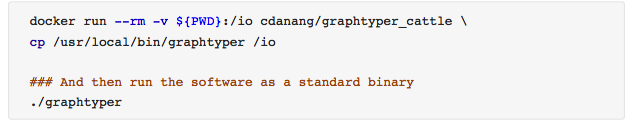
\includegraphics[width=\textwidth]{paper1/supplement/sp12.png}
\end{figure}

If you prefer to modify and build a modified version of Graphtyper for the bovine chromosome
complement directly from the source, please follow the instructions below:

\begin{enumerate}
    \item Clone the \emph{Graphtyper Github}
    \begin{figure}[!htb]
        \centering
        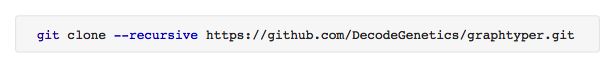
\includegraphics[width=\textwidth]{paper1/supplement/sp13.png}
    \end{figure}

    \item Create a new \emph{branch} at this specific commit tag. We built graphtyper at this specific
    commit hash (04ab5ee460fa36129fb0d8ea5d4b72adc3836f52), to compile at the same
    software version that we use in the paper, please use this commit tag. We named the
    branch as \emph{cattle modification}

    \begin{figure}[!htb]
        \centering
        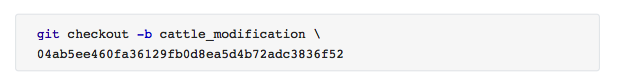
\includegraphics[width=\textwidth]{paper1/supplement/sp14.png}
    \end{figure}

    \item Change directory into \emph{graphtyper} and modify the chromosomal specifications in the files
    include $graphtyper/graph/absolute_position.hpp$ and $src/typer/vcf.cpp$ using UMD 3.1 cattle
    chromosomal names and lengths. The first modification enables all cattle chromosomes
    (esp. for chromosome number $>$ 23) as the current software release set the maximum
    allowed length for each chromosomes according to the human GRChb37 and GRCh38. The
    second modifications are required that the respective chromosomal information is written
    to the \emph{vcf header}.

    \item Make sure that these dependencies are installed:
    \begin{itemize}
        \item C++ compiler with C++11 supported (we tested gcc 4.8.5 or gcc 6.3.0 
        \item Boost$\geq$1.57.0
        \item zlib$\geq$1.2.8
        \item libbz2
        \item liblzma
        \item Autotools, Automake, libtool, Make, and CMake>=2.8.8
    \end{itemize}
    
    \item Follow installation procedures as below. This will put the software in \emph{releasebuild/bin/graphtyper}
    
    \begin{figure}[!htb]
        \centering
        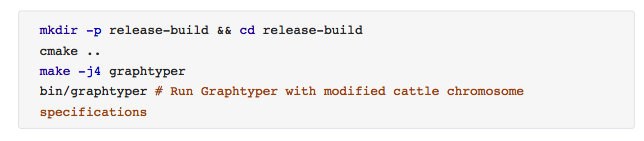
\includegraphics[width=\textwidth]{paper1/supplement/sp15.png}
    \end{figure}

\end{enumerate}

\newpage

\subsection{}
\label{supp_mat:22}
\textbf{\large{Properties of the different metrics used for the evaluation of sequence variant genotyping accuracy.}}


The metrics were calculated using the sum of the red cells as numerator and the cells within the green frame as denominator.
\bigskip
\bigskip
\bigskip

\begin{figure}[!htb]
    \centering
    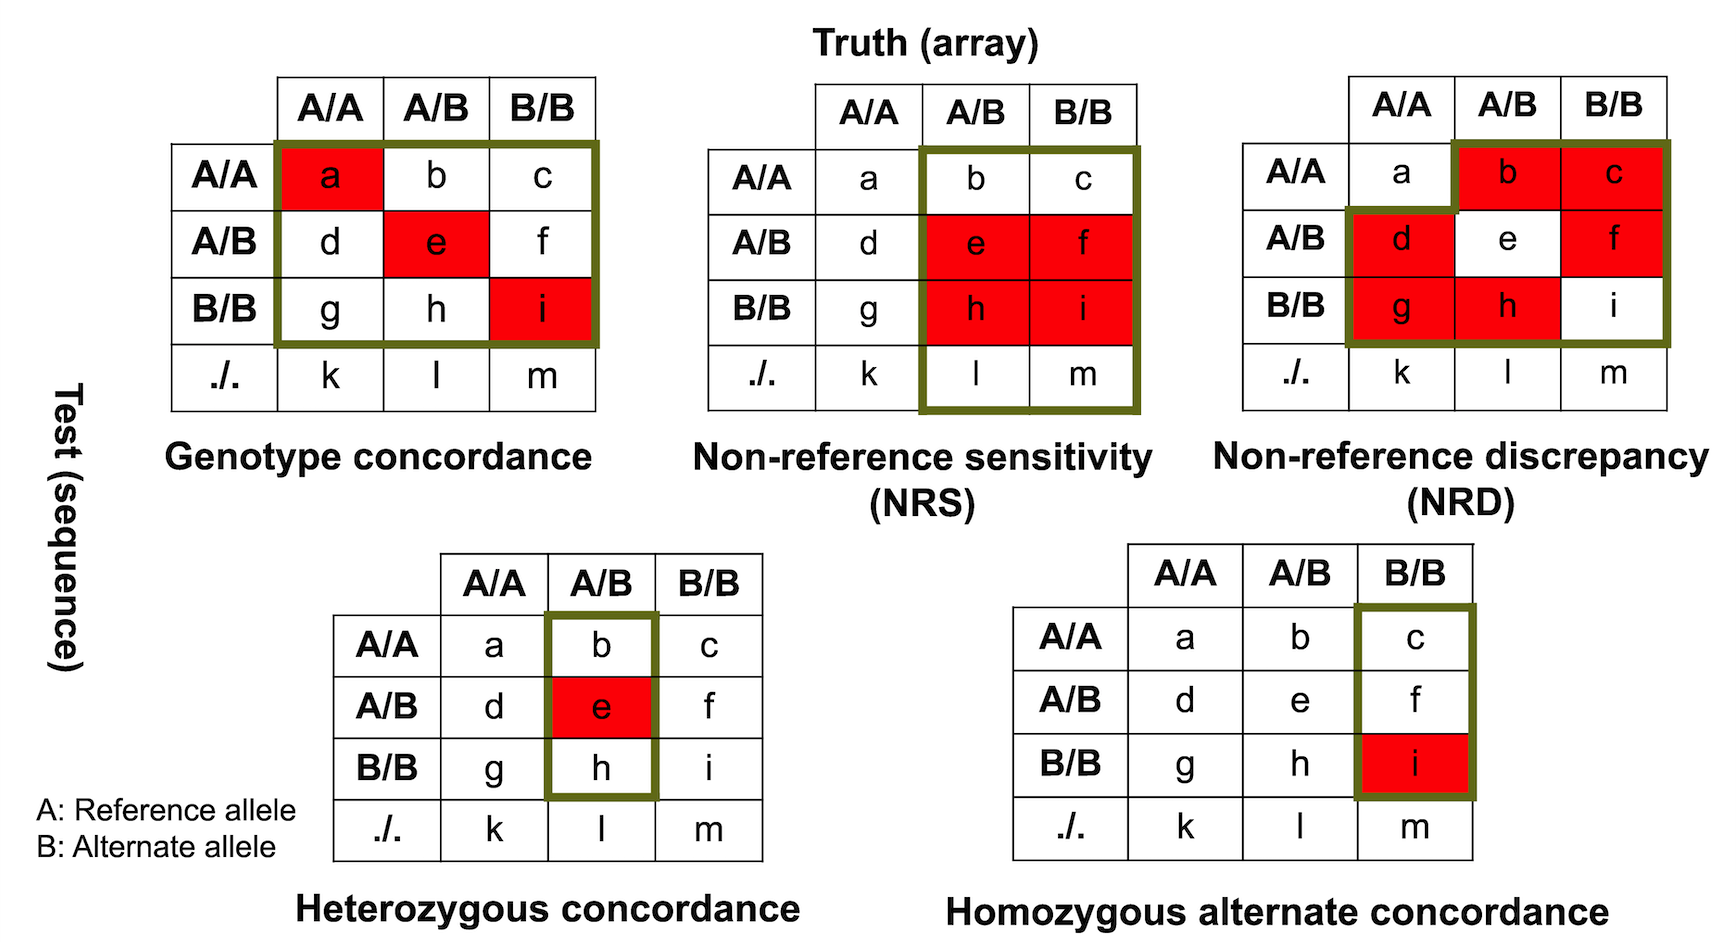
\includegraphics[width=\textwidth]{paper1/supplement/sp2.png}
\end{figure}

\newpage

\begin{landscape}


\subsection{}
\label{supp_mat:23}
\textbf{\large{Concordance statistics}}


The concordance of heterozygous and alternate homozygous genotypes in 49 Original Braunvieh cattle (\textbf{a}) and the concordance at the different sequencing depth for the (\textbf{b}) raw and (\textbf{c}) imputed datasets.

\bigskip
\bigskip
\bigskip

    
    \begin{figure}[!htb]
        \centering
        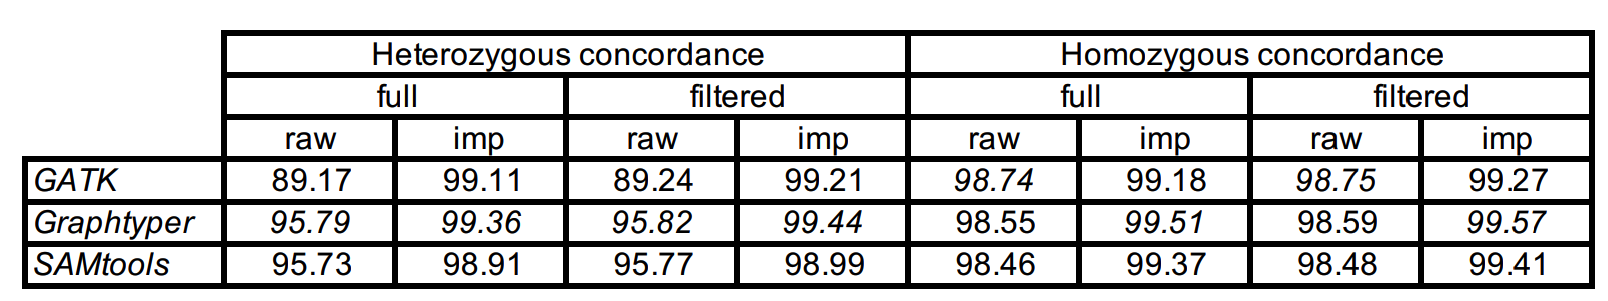
\includegraphics[width=1.4\textwidth]{paper1/supplement/sp31.png}
    \end{figure} 

    \begin{figure}[!htb]
        \centering
        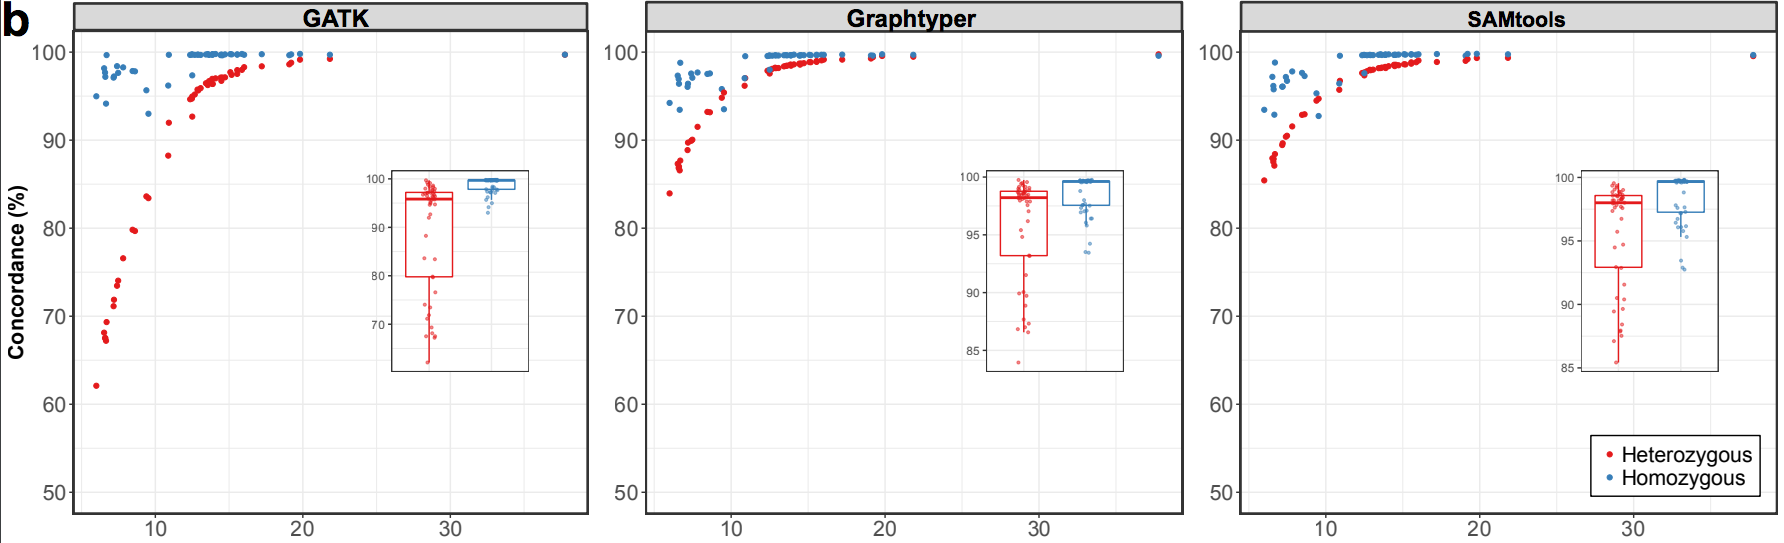
\includegraphics[width=1.5\textwidth]{paper1/supplement/sp32.png}
        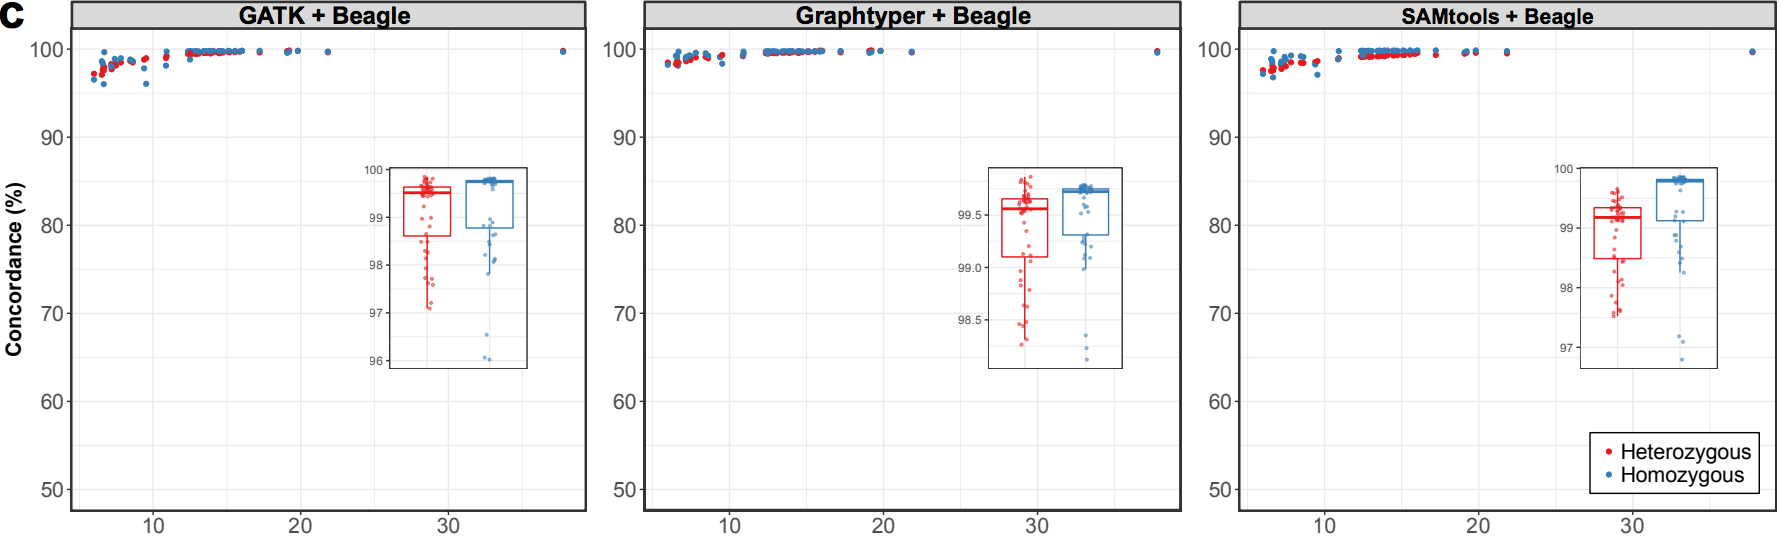
\includegraphics[width=1.5\textwidth]{paper1/supplement/sp33.png}
    \end{figure}

\newpage


\subsection{}
\label{supp_mat:24}
\textbf{\large{Sequence variant genotyping quality for 18 and 31 animals that were sequenced at a lower and higher than 12-fold sequencing coverage, respectively.}}

Asterisks denote significant differences with the best value (italic) for a respective parameter.

\bigskip
\bigskip
\bigskip


    
    \centering
    \emph{Coverage less than 12}
    \begin{footnotesize}
    \arrayrulecolor{black}
    \begin{tabular}{|l|c|c|c|c|c|c|c|c|c|c|c|c|} 
    \cline{2-13}
    \multicolumn{1}{c|}{\multirow{3}{*}{}} & \multicolumn{4}{c|}{Genotype concordance}                 & \multicolumn{4}{c|}{Non-reference sensitivity}            & \multicolumn{4}{c|}{Non-reference discrepancy}             \\ 
    \cline{2-13}
    \multicolumn{1}{c|}{}                  & \multicolumn{2}{c|}{full} & \multicolumn{2}{c|}{filtered} & \multicolumn{2}{c|}{full} & \multicolumn{2}{c|}{filtered} & \multicolumn{2}{c|}{full} & \multicolumn{2}{c|}{filtered}  \\ 
    \cline{2-13}
    \multicolumn{1}{c|}{}                  & raw      & imp~           & raw      & imp                & raw      & imp            & raw      & imp                & raw      & imp            & raw      & imp                 \\ 
    \arrayrulecolor{black}\cline{1-1}\arrayrulecolor{black}\cline{2-13}
    GATK                                   & 90.99*** & 98.7***        & 91.02*** & 98.82***           & 85.63*** & 98.91          & 85.51*** & 98.73              & 14.64*** & 2.09***        & 14.59*** & 1.91***             \\ 
    \hline
    Graphtyper                             & 94.89    & 99.07          & 94.91    & 99.17              & 96.44    & 99             & 96.13    & 98.71              & 8.04     & 1.49           & 8        & 1.31                \\ 
    \hline
    SAMtools                               & 94.87    & 98.61***       & 94.89    & 98.67***           & 96.24*** & 98.94          & 95.75*** & 98.45***           & 8.11     & 2.24***        & 8.09     & 2.11***             \\
    \hline
    \end{tabular}
    \end{footnotesize}


\bigskip
\bigskip

    \centering
    \emph{Coverage more than 12}
    \begin{footnotesize}
    \arrayrulecolor{black}
    \begin{tabular}{|l|c|c|c|c|c|c|c|c|c|c|c|c|} 
    \cline{2-13}
    \multicolumn{1}{c|}{\multirow{3}{*}{}} & \multicolumn{4}{c|}{Genotype concordance}                 & \multicolumn{4}{c|}{Non-reference sensitivity}            & \multicolumn{4}{c|}{Non-reference discrepancy}             \\ 
    \cline{2-13}
    \multicolumn{1}{c|}{}                  & \multicolumn{2}{c|}{full} & \multicolumn{2}{c|}{filtered} & \multicolumn{2}{c|}{full} & \multicolumn{2}{c|}{filtered} & \multicolumn{2}{c|}{full} & \multicolumn{2}{c|}{filtered}  \\ 
    \cline{2-13}
    \multicolumn{1}{c|}{}                  & raw      & imp~           & raw      & imp                & raw     & imp             & raw      & imp                & raw     & imp             & raw     & imp                  \\ 
    \arrayrulecolor{black}\cline{1-1}\arrayrulecolor{black}\cline{2-13}
    GATK                                   & 98.73*** & 99.66          & 98.76*** & 99.71              & 98.3*** & 99.61           & 98.14*** & 99.39              & 1.8***  & 0.48*           & 1.76*** & 0.42                 \\ 
    \hline
    Graphtyper                             & 99.26    & 99.67          & 99.3     & 99.72              & 99.25   & 99.54***        & 98.88    & 99.16***           & 1.04    & 0.45            & 0.99    & 0.4                  \\ 
    \hline
    SAMtools                               & 99.21*** & 99.59***       & 99.24*** & 99.62***           & 99.21** & 99.58***        & 98.51*** & 98.79***           & 1.12*** & 0.58***         & 1.08*** & 0.54***              \\
    \hline
    \end{tabular}
    \end{footnotesize}


\end{landscape}

\newpage

\subsection{}
\label{supp_mat:25}
\textbf{\large{Twelve 1-Mb regions for which \emph{Graphtyper} initially failed to genotype sequence variants}}

The algorithm either ran out of memory or exceeded the allocated runtime (12 h). Graphtyper eventually produced genotypes for the sequence variants when these regions were re-run in 10-kb segments.

\bigskip
\bigskip
\bigskip

\begin{center}
    \begin{tabular}{|c|c|c|} 
        \hline
        No & Chromosome & Region (Mb)  \\ 
        \hline
        1  & 1          & 0-1          \\ 
        \hline
        2  & 1          & 145-146      \\ 
        \hline
        3  & 3          & 69-70        \\ 
        \hline
        4  & 7          & 58-57        \\ 
        \hline
        5  & 8          & 110-111      \\ 
        \hline
        6  & 12         & 76-77        \\ 
        \hline
        7  & 23         & 26-27        \\ 
        \hline
        8  & 23         & 29-30        \\ 
        \hline
        9  & 26         & 50-51        \\ 
        \hline
        10 & 27         & 37-38        \\ 
        \hline
        11 & 28         & 39-40        \\ 
        \hline
        12 & 29         & 30-31        \\
        \hline
        \end{tabular}
\end{center}

\newpage
\subsection{}
\label{supp_mat:26}
\textbf{\large{Variant filtration using \emph{GATK}}}
\bigskip

The best practice guidelines for variant discovery using \emph{GATK} recommend sequence
variants to be filtered using Variant Quality Score Recalibration (VQSR) because it
implements advanced machine learning-based methods to differentiate between true and
false-positive variants. However, VQSR relies on sets of high confidence truth/training
variants, which are currently not (publicly) available in cattle. Thus, we ran \emph{GATK} with best
practice recommendations for variant filtering when applying VQSR is not possible, i.e., we
used a generic baseline hard-filtering threshold for each variant annotation (see
\url{https://gatkforums.broadinstitute.org/GATK/discussion/2806/howto-apply-hard-filters-to-acall-set}). This threshold-based filtering is commonly applied the cattle genomics community
\citep{koufariotis2018sequencing,chen2018whole}
\bigskip



To facilitate running the VQSR module in sheep and goat, i.e., species where sets of
truth/training variants are not (publicly) available, \citep{alberto2018convergent} used an
intersection of high confidence variants that had been discovered from multiple variant
callers as truth/training sets, i.e., they derived truth/training sets directly from the analyzed
data. We implemented their approach to apply \emph{GATK} VQSR to our variant dataset. Training
and truth sets were constructed using the overlap of the filtered variants from the GATK,
\emph{Graphtyper} and \emph{SAMtools} pipelines (truth=false, training=true, known=false, prior= 10) and
markers from the BovineHD BeadChip (truth=true, training=true, known=false, prior= 15),
respectively. Moreover, we used variants listed in dbSNP (version 150) as known variants
(truth=false, training=false, known=true, prior=3.0). Following \emph{GATK} VQSR, we retained
variants in the 99.9\% tranche sensitivity threshold (best practice).

\bigskip

Variant filtration using \emph{GATK} VQSR removed more variants from the raw data than \emph{GATK}
hard filtering (Table 1). However, VQSR retained more HD SNPs than \emph{GATK} hard filtering,
possibly reflecting bias that results from the use of HD SNPs as training/truth sets. The
values of the concordance statistics (genotype concordance, non-reference sensitivity, nonreference discrepancy) were almost identical between \emph{GATK} VQSR and \emph{GATK} hard
filtration (Table 2) indicating that the choice of either filtration option does not notably affect
the concordance between sequence-derived and BovineHD SNP array-derived genotypes.
These findings are in line with \citep{vander2018best} who showed that the concordance
between microarray-called and sequence-derived genotypes is almost identical using either
\emph{GATK} VQSR or the \emph{GATK} 1000 bull genomes project hard filters, even though they used
stringently filtered truth/training sets based on a more comprehensive catalogue of variants
than in our study. Interestingly, in agreement with \citep{vander2018best}, the proportion
of opposing homozygous genotypes in sire/son-pairs (which does not suffer from
ascertainment bias because it is calculated using sequence-derived SNPs) is less using
\emph{GATK} hard filter than \emph{GATK} VQSR.

\bigskip

The performance of \emph{GATK} VQSR may be assessed using the novel variant sensitivity
tranche plot (Figure 2). In the lowest 90\% tranches (highest specificity) the filtering model
still retained many false positive variants (orange box and low Ti/Tv ratio). However, when
the 99.9\% tranche sensitivity is used as filtration criterion as recommended by the \emph{GATK}
best practice guidelines, a high proportion of true positive variants is removed from the
data. 

Overall, our findings suggest that

\begin{enumerate}[(i)]
    \item \emph{GATK} VQSR removes more variants from the data than \emph{GATK} hard filtering,
    \item \emph{GATK} VQSR does not notably improve the concordance between sequencederived and microarray-called genotypes compared to \emph{GATK} hard filtering,
    \item the proportion of opposing homozygous genotypes in sire/son-pairs is higher using \emph{GATK} VQSR than \emph{GATK} hard filtering, and
    \item improving VQSR may be possible by providing more sophisticated truth/training variant datasets produced by orthogonal sequencing technology other than the ones used for training, e.g. \citep{li2018synthetic}
\end{enumerate}

\textbf{Table 1} Comparison of variants statistics between unfiltered and filtered datasets using
either hard-filtering or VQSR.


\bigskip

\begin{center}
\begin{tabular}{|l|l|l|l|} 
    \cline{2-4}
    \multicolumn{1}{l|}{~} & \textit{GATK} full & \textit{GATK }hard-filter & \textit{GATK} VQSR  \\ 
    \hline
    Total SNPs             & 18,594,182         & 17,248,593                & 16,537,577          \\ 
    \hline
    Biallelic              & 18,347,962         & 17,111,806                & 16,430,734          \\ 
    \hline
    Multi-allelic          & 246,220            & 136,787                   & 106,843             \\ 
    \hline
    Ti/Tv ratio            & 2.09               & 2.17                      & 2.16                \\ 
    \hline
    BovineHD               & 99.46              & 99.21                     & 99.38               \\ 
    \hline
    BovineSNP50            & 99.14              & 98.91                     & 98.98               \\
    \hline
    \end{tabular}
\end{center}

\bigskip

\textbf{Table 2} The concordance statistics between hard-filtered and VQSR 

\bigskip

\begin{tabular}{|c|c|c|c|c|} 
    \cline{2-5}
    \multicolumn{1}{c|}{~}    & \begin{tabular}[c]{@{}c@{}}Genotype \\concordance\end{tabular} & \begin{tabular}[c]{@{}c@{}}Non-reference \\sensitivity\end{tabular} & \begin{tabular}[c]{@{}c@{}}Non-reference \\discrepancy\end{tabular} & \begin{tabular}[c]{@{}c@{}}Opposing\\Homozygous\end{tabular}  \\ 
    \hline
    \textit{GATK} hard-filter & 96.02                                                          & 93.67                                                               & 6.3                                                                 & 0.72                                                          \\ 
    \hline
    \textit{GATK} VQSR        & 96.01                                                          & 93.77                                                               & 6.32                                                                & 0.75                                                          \\
    \hline
\end{tabular}

\bigskip
\bigskip


\textbf{Figure 1} Tranche sensitivity plot of novel variants as reported by the VQSR model fitting

\begin{figure}[!htb]
    \centering
    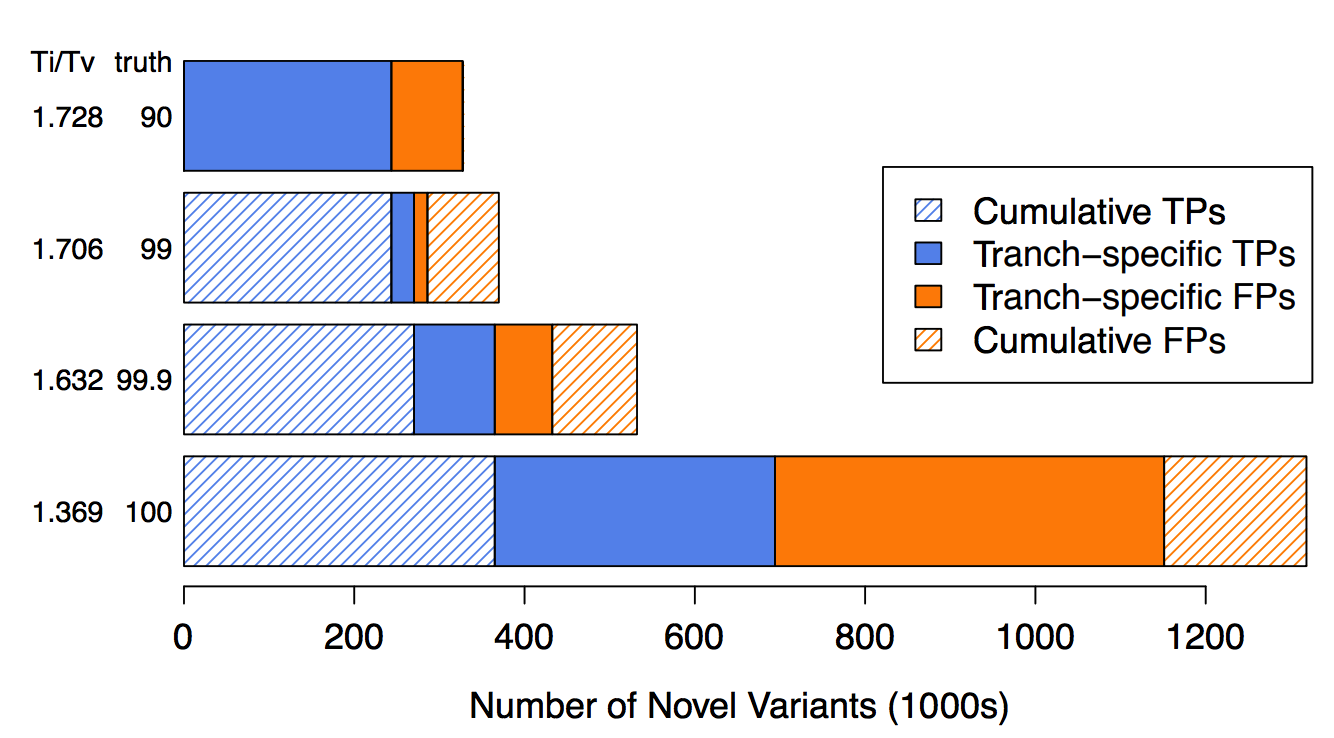
\includegraphics[width=\textwidth]{paper1/supplement/sp6.png}
\end{figure}

\newpage

\begin{landscape}
\subsection{}
\label{supp_mat:27}
\textbf{\large{Accuracy and sensitivity of sequence variant genotyping on bovine chromosome 25 from a variation-aware genome graph that incorporated 2,143,417 dbSNP variants as prior known variants.}}
\bigskip


    \begin{figure}[!htb]
        \centering
        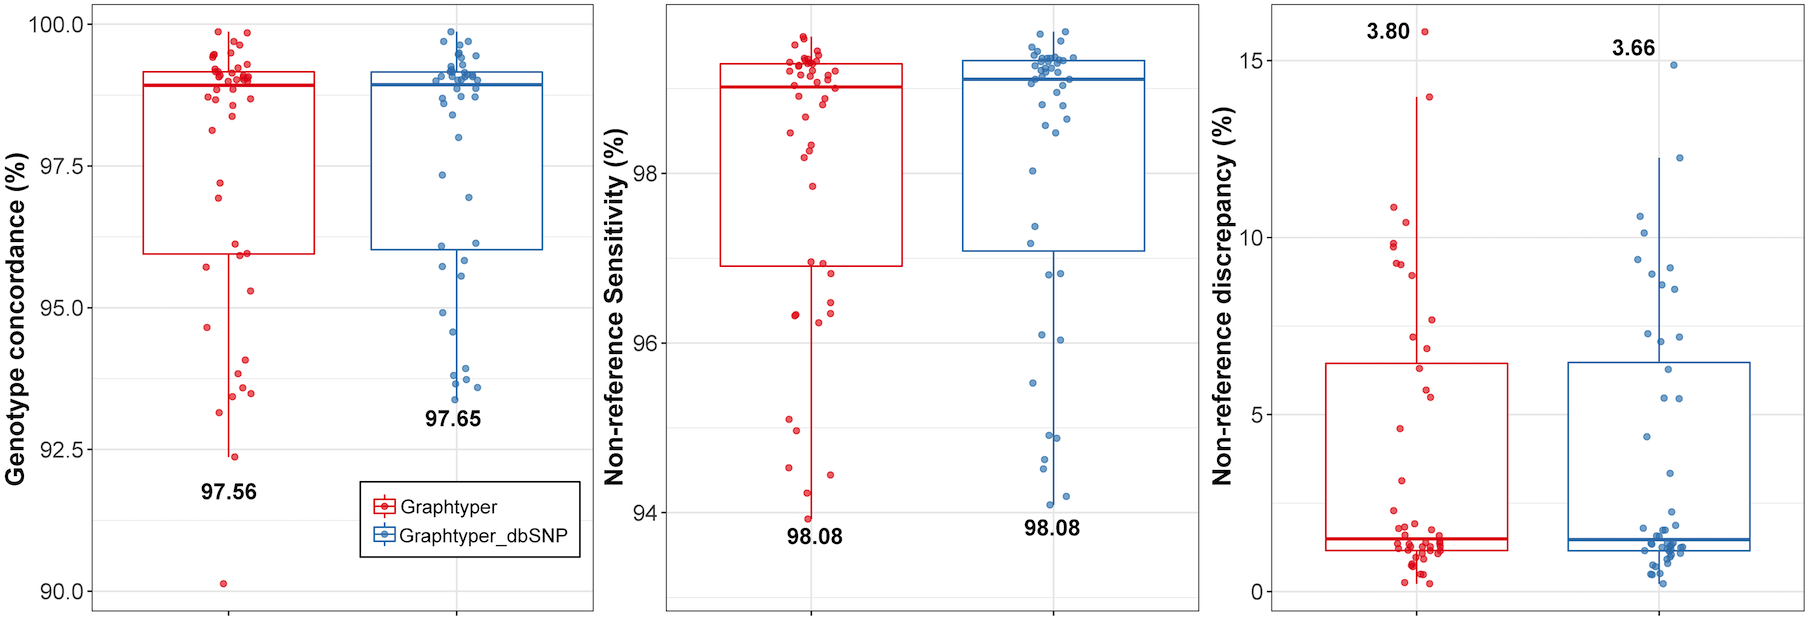
\includegraphics[width=1.5\textwidth]{paper1/supplement/sp7.png}
    \end{figure}
\end{landscape}


\renewcommand{\bibname}{Supplementary References}
\bibliographystyle{abbrvnat}
\bibliography{references/chapter2_ref}

\end{flushleft}

\ifdefined\BuildingFromMainFile
\else
   \end{document}
\fi


\chapter*{\centering{Supplementary Materials \\ Chapter \ref{chap:wholegraph}}}
\addcontentsline{toc}{chapter}{Supplementary Materials Chapter 3}
\singlespacing
\fancyhead[C]{APPENDICES}
\ifdefined\BuildingFromMainFile
\else
   \documentclass[../main.tex]{subfiles}
   \graphicspath{{figure/}{../figure/}}
   \begin{document}
\fi


\newpage

\setcounter{subsection}{0}
\renewcommand \thesubsection {Note S3.\arabic{subsection}}
\setcounter{figure}{0}
\renewcommand \thefigure {S3.\arabic{figure}}
\setcounter{table}{0}
\renewcommand \thetable {S3.\arabic{table}}

\begin{flushleft}
    
\begin{figure}[!htb]
    \centering
    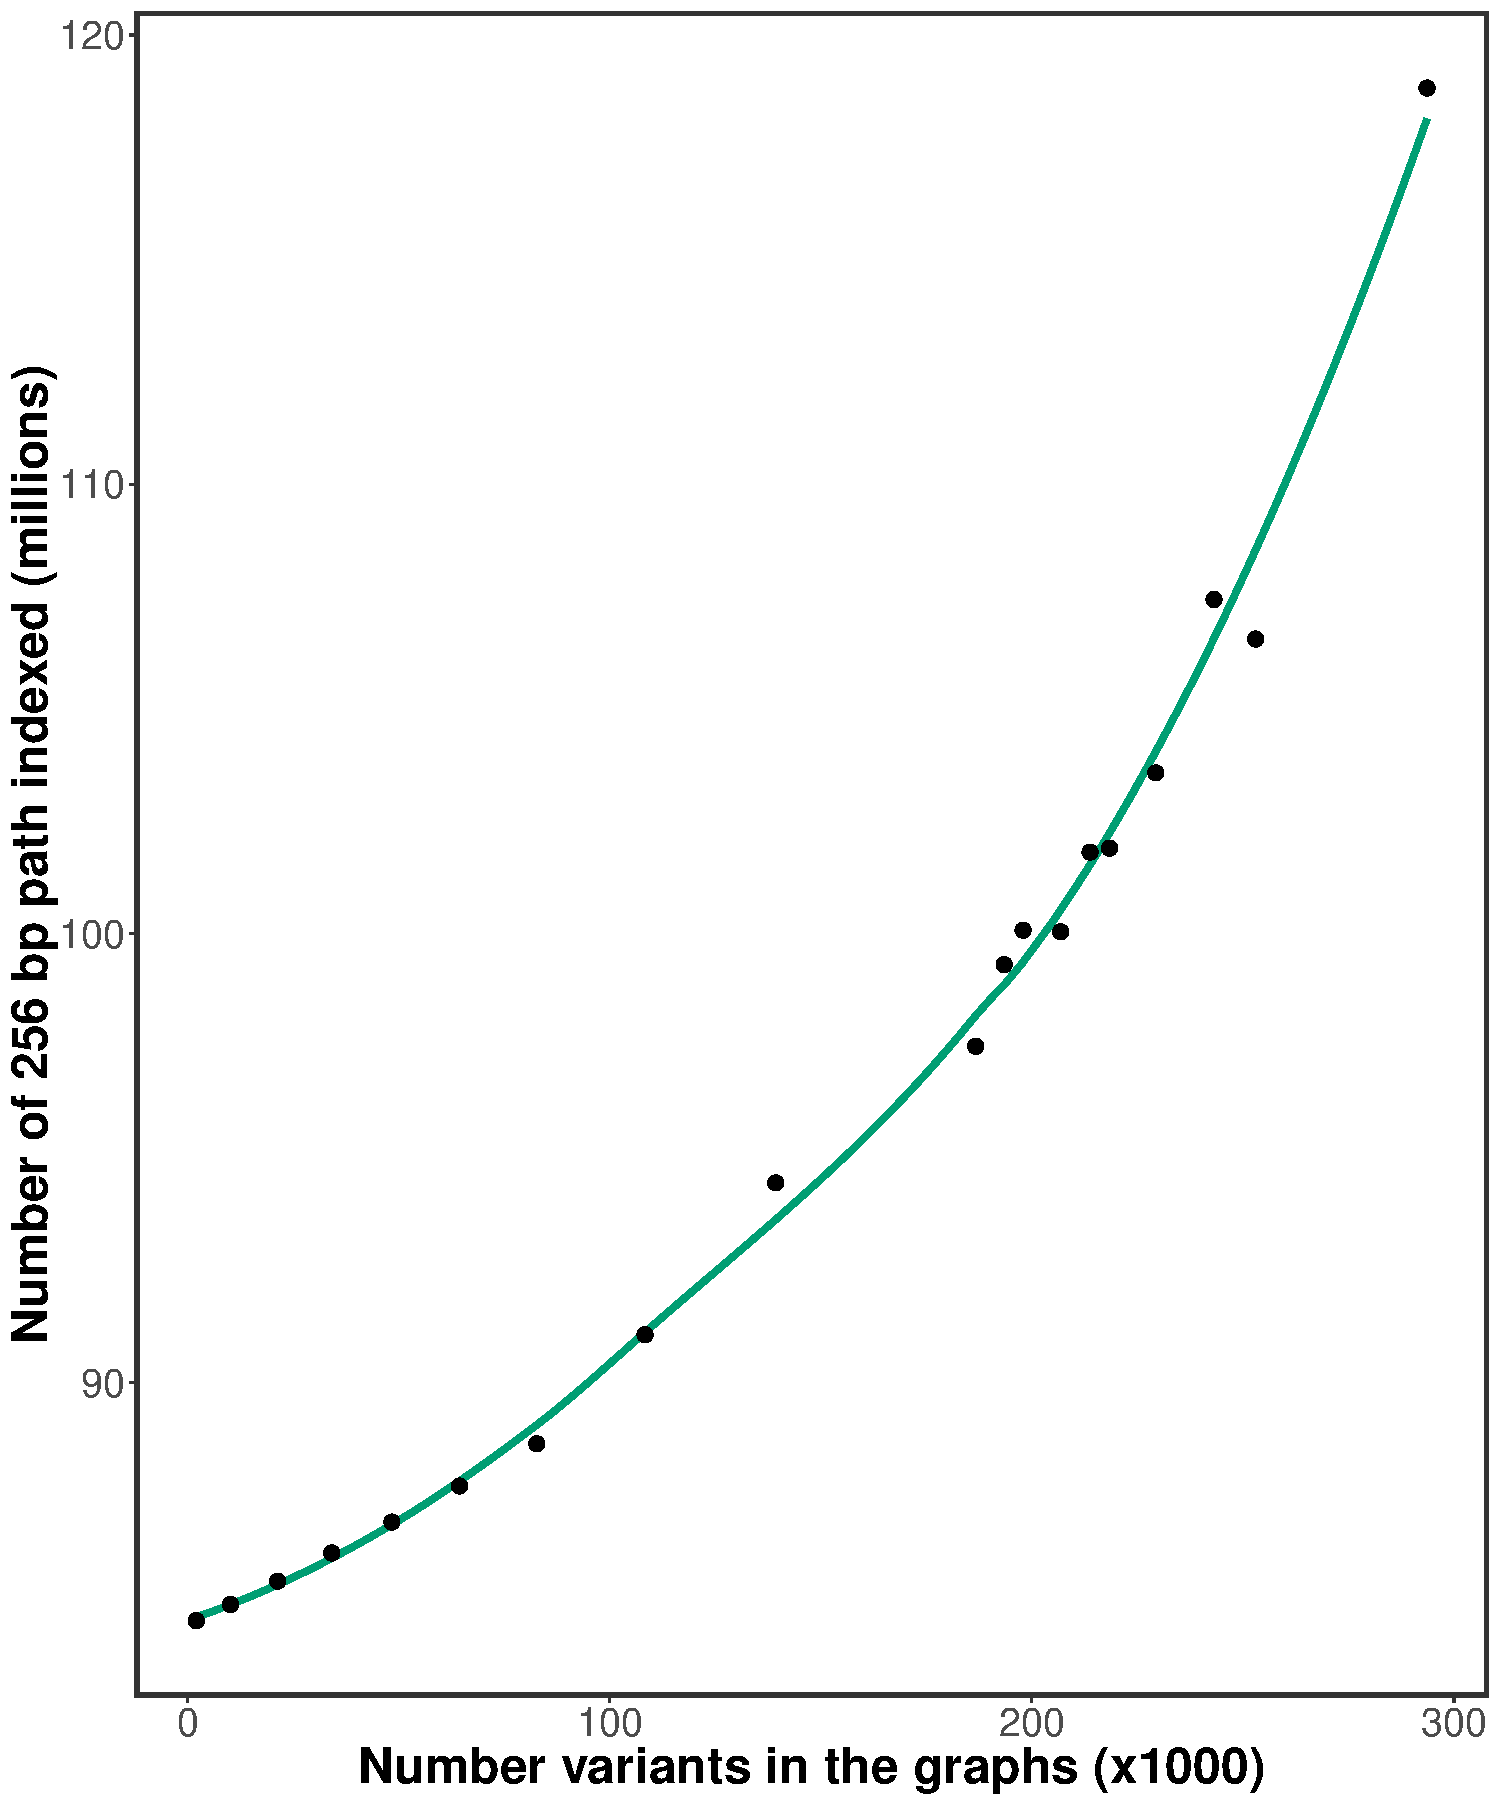
\includegraphics[width=0.7\textwidth]{paper2/supplement/sp31.pdf}
    \caption[Number of 256 bp haplotype paths]{\textbf{Number of 256 bp haplotype paths in the graphs with an increasing
    number of variants added to the graphs.} \\
    \small{The line plot is fitted using loess function in \emph{R}.}}
    \label{sup_fig:s31}
\end{figure}


\newpage

\begin{figure}[!htb]
    \centering
    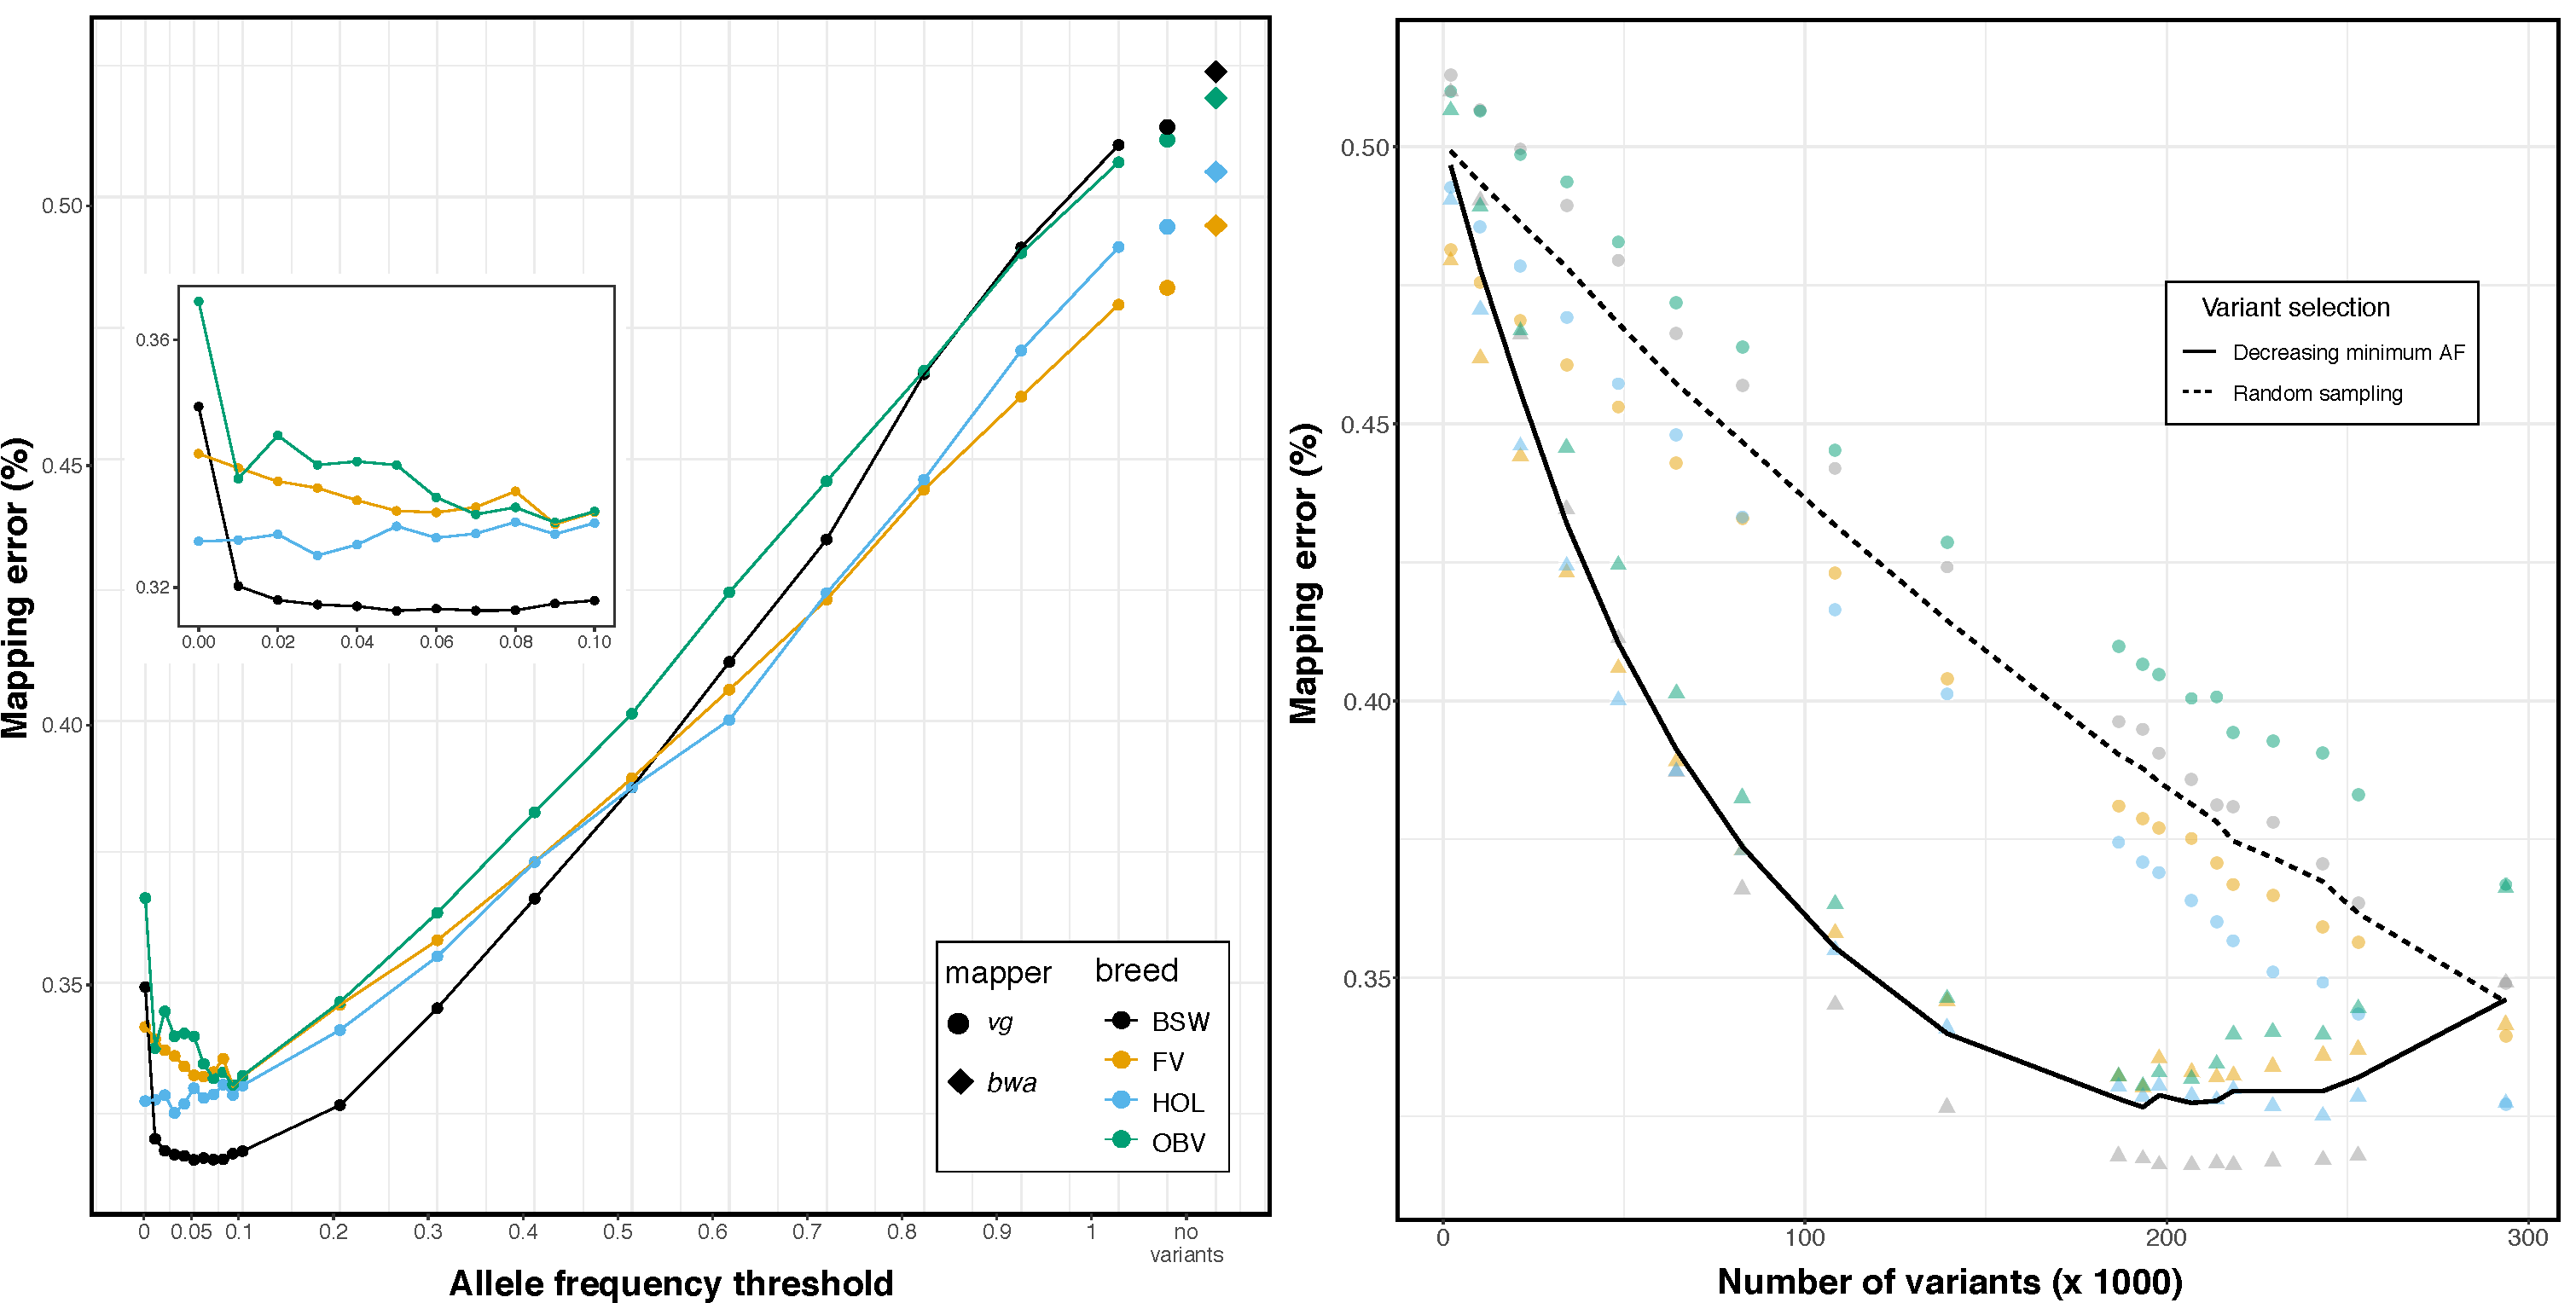
\includegraphics[width=\textwidth]{paper2/supplement/sp32.pdf}
    \caption[Single-end mapping accuracy]{\textbf{Single-end mapping accuracy using genome graphs that contained
    variants filtered for allele frequency.} \\
    \small{(a) Proportion of incorrectly mapped reads for four breed-specific augmented
    genome graphs. Diamonds and large dots represent results from linear mapping
    using \emph{BWA mem} and \emph{vg}, respectively. The inset is a larger representation of the
    mapping accuracy for alternate allele frequency thresholds less than 0.1. (b) Read
    mapping accuracy for breed-specific augmented graphs that contained variants that
    were either filtered for alternate allele frequency (triangles) or sampled randomly
    (circles) from all variants detected within a breed. The dashed and solid line
    represents the average proportion of mapping errors across four breeds using
    variant prioritization and random sampling. }}
    \label{sup_fig:s32}
\end{figure}


\begin{figure}[!htb]
    \centering
    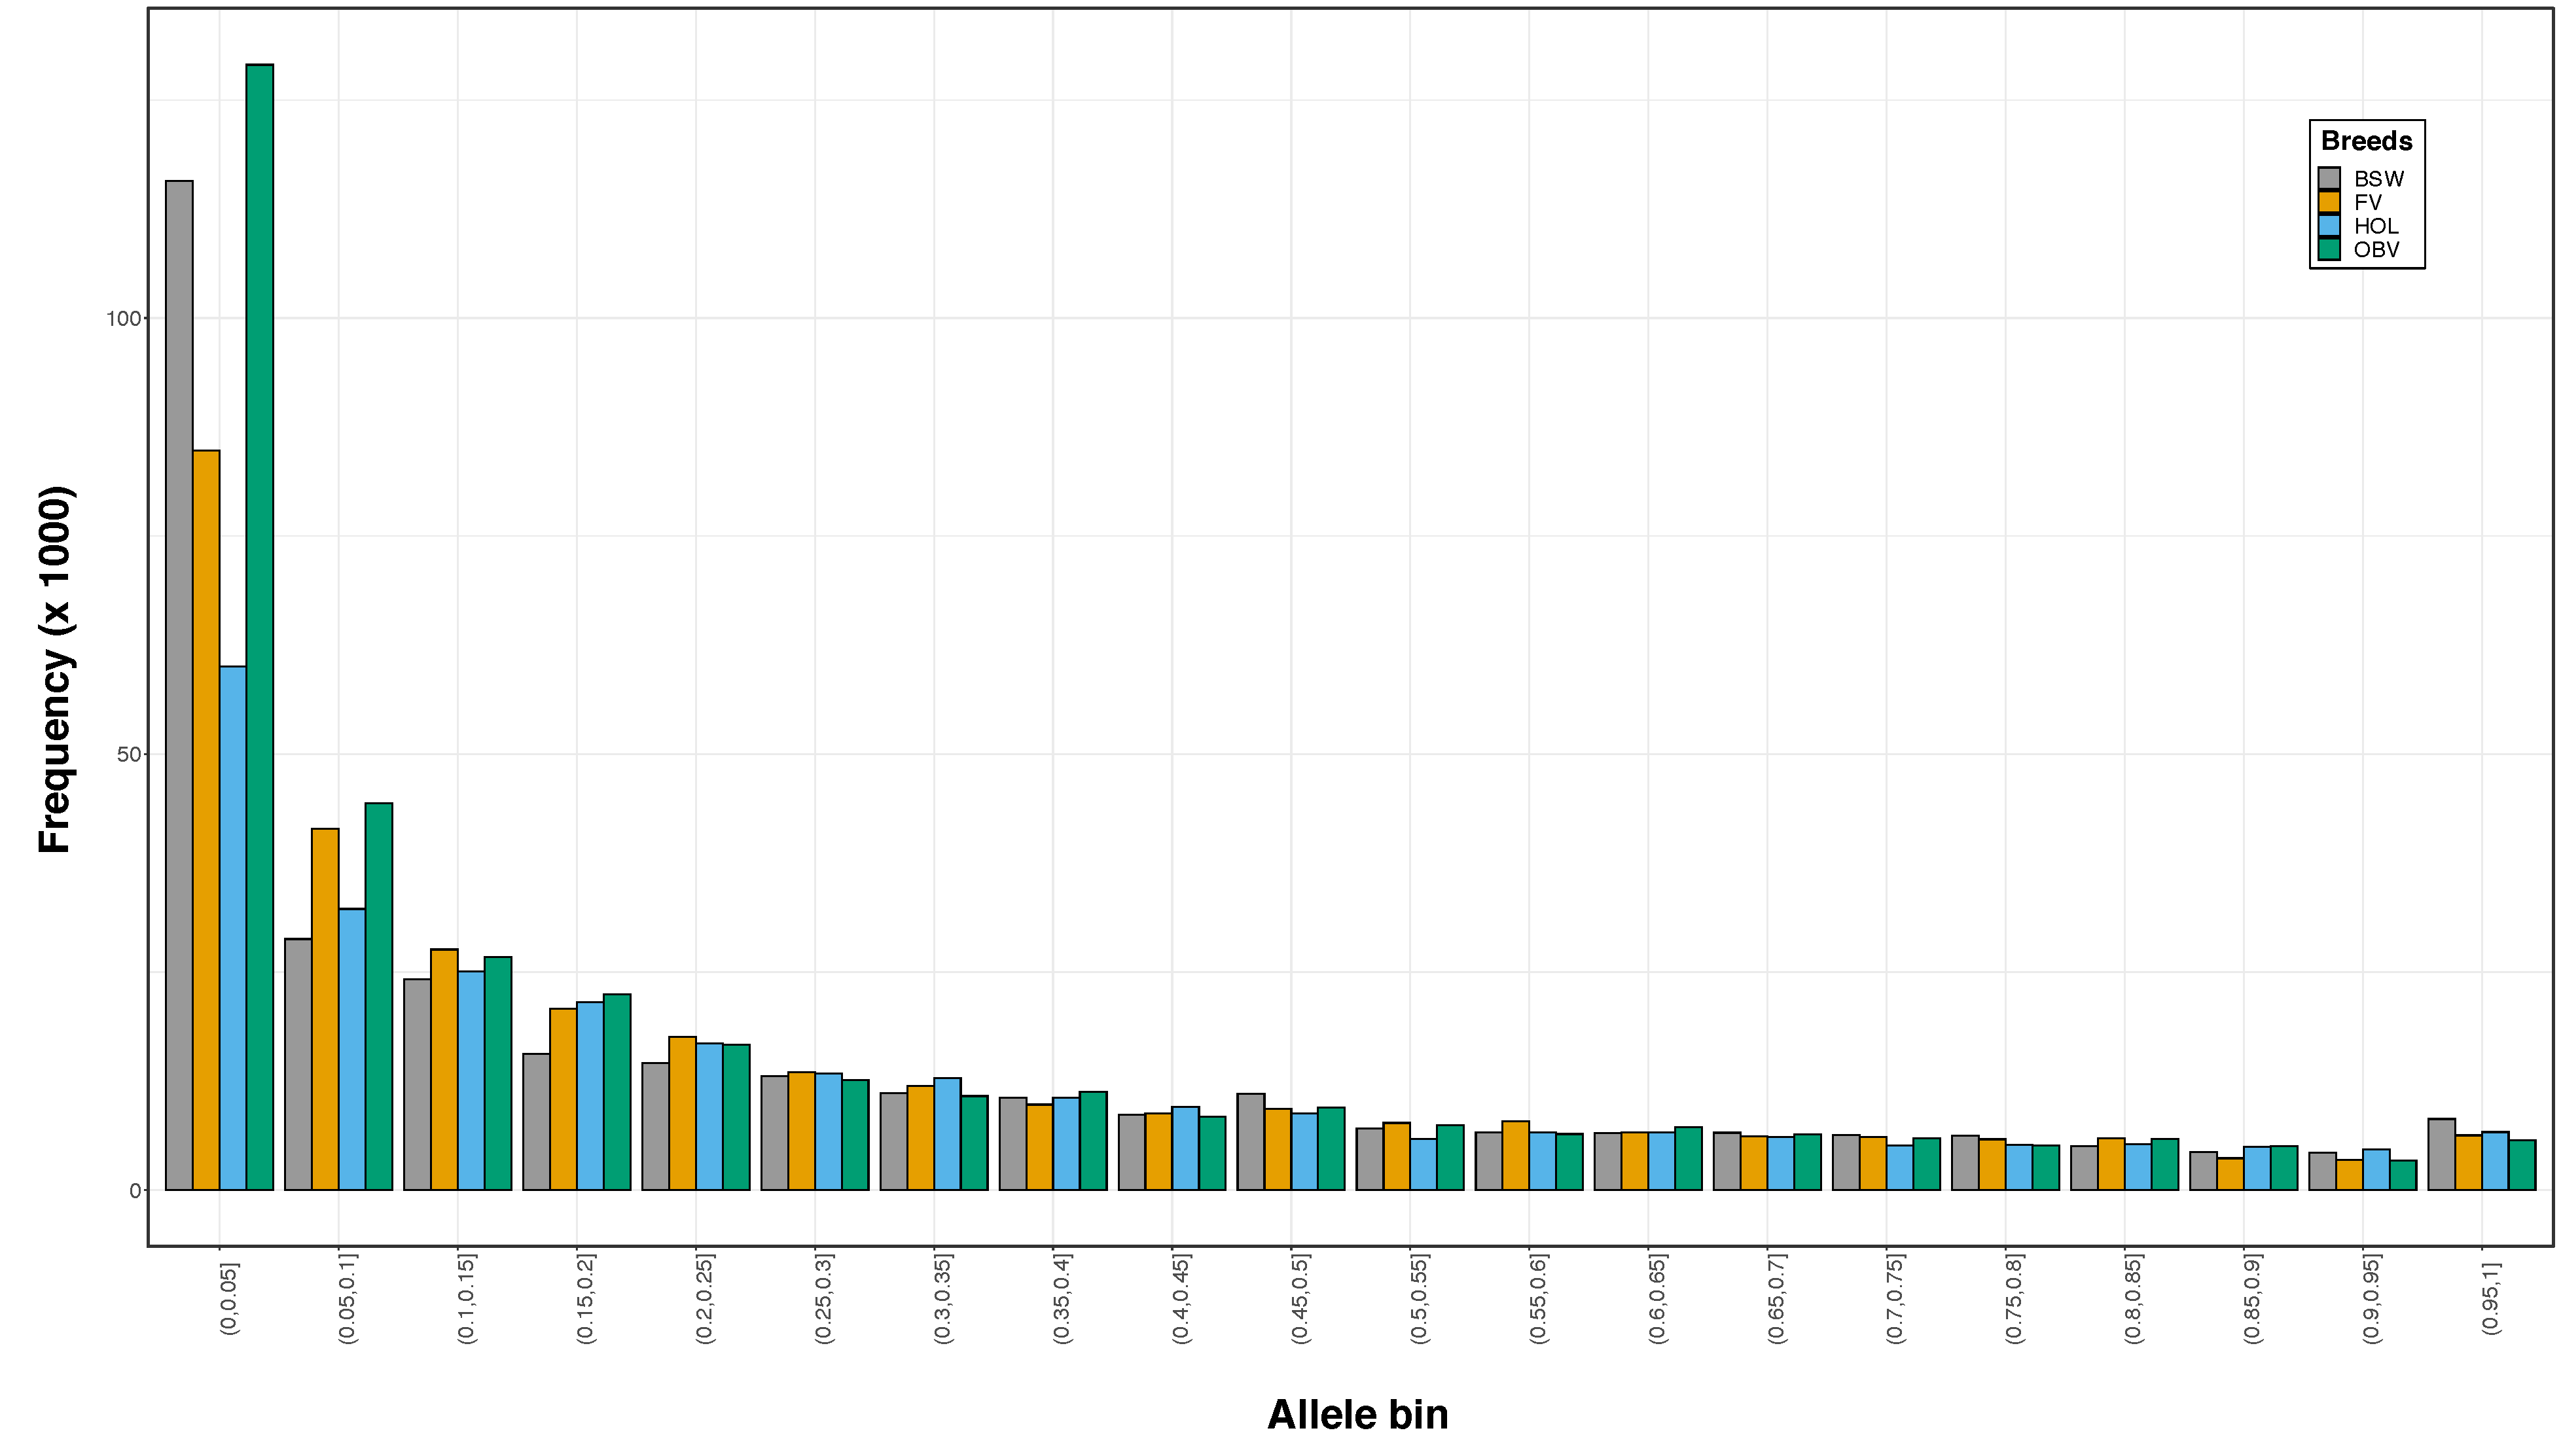
\includegraphics[width=\textwidth]{paper2/supplement/sp33.pdf}
    \caption[Number of variants detected on chromosome 25]{\textbf{Number of variants detected on chromosome 25 in 82 BSW, 49 FV,
    49 HOL and 108 OBV cattle.} \\
    \small{Variants are binned according to allele frequency.}}
    \label{sup_fig:s33}
\end{figure}

\newpage

\begin{figure}[!htb]
    \centering
    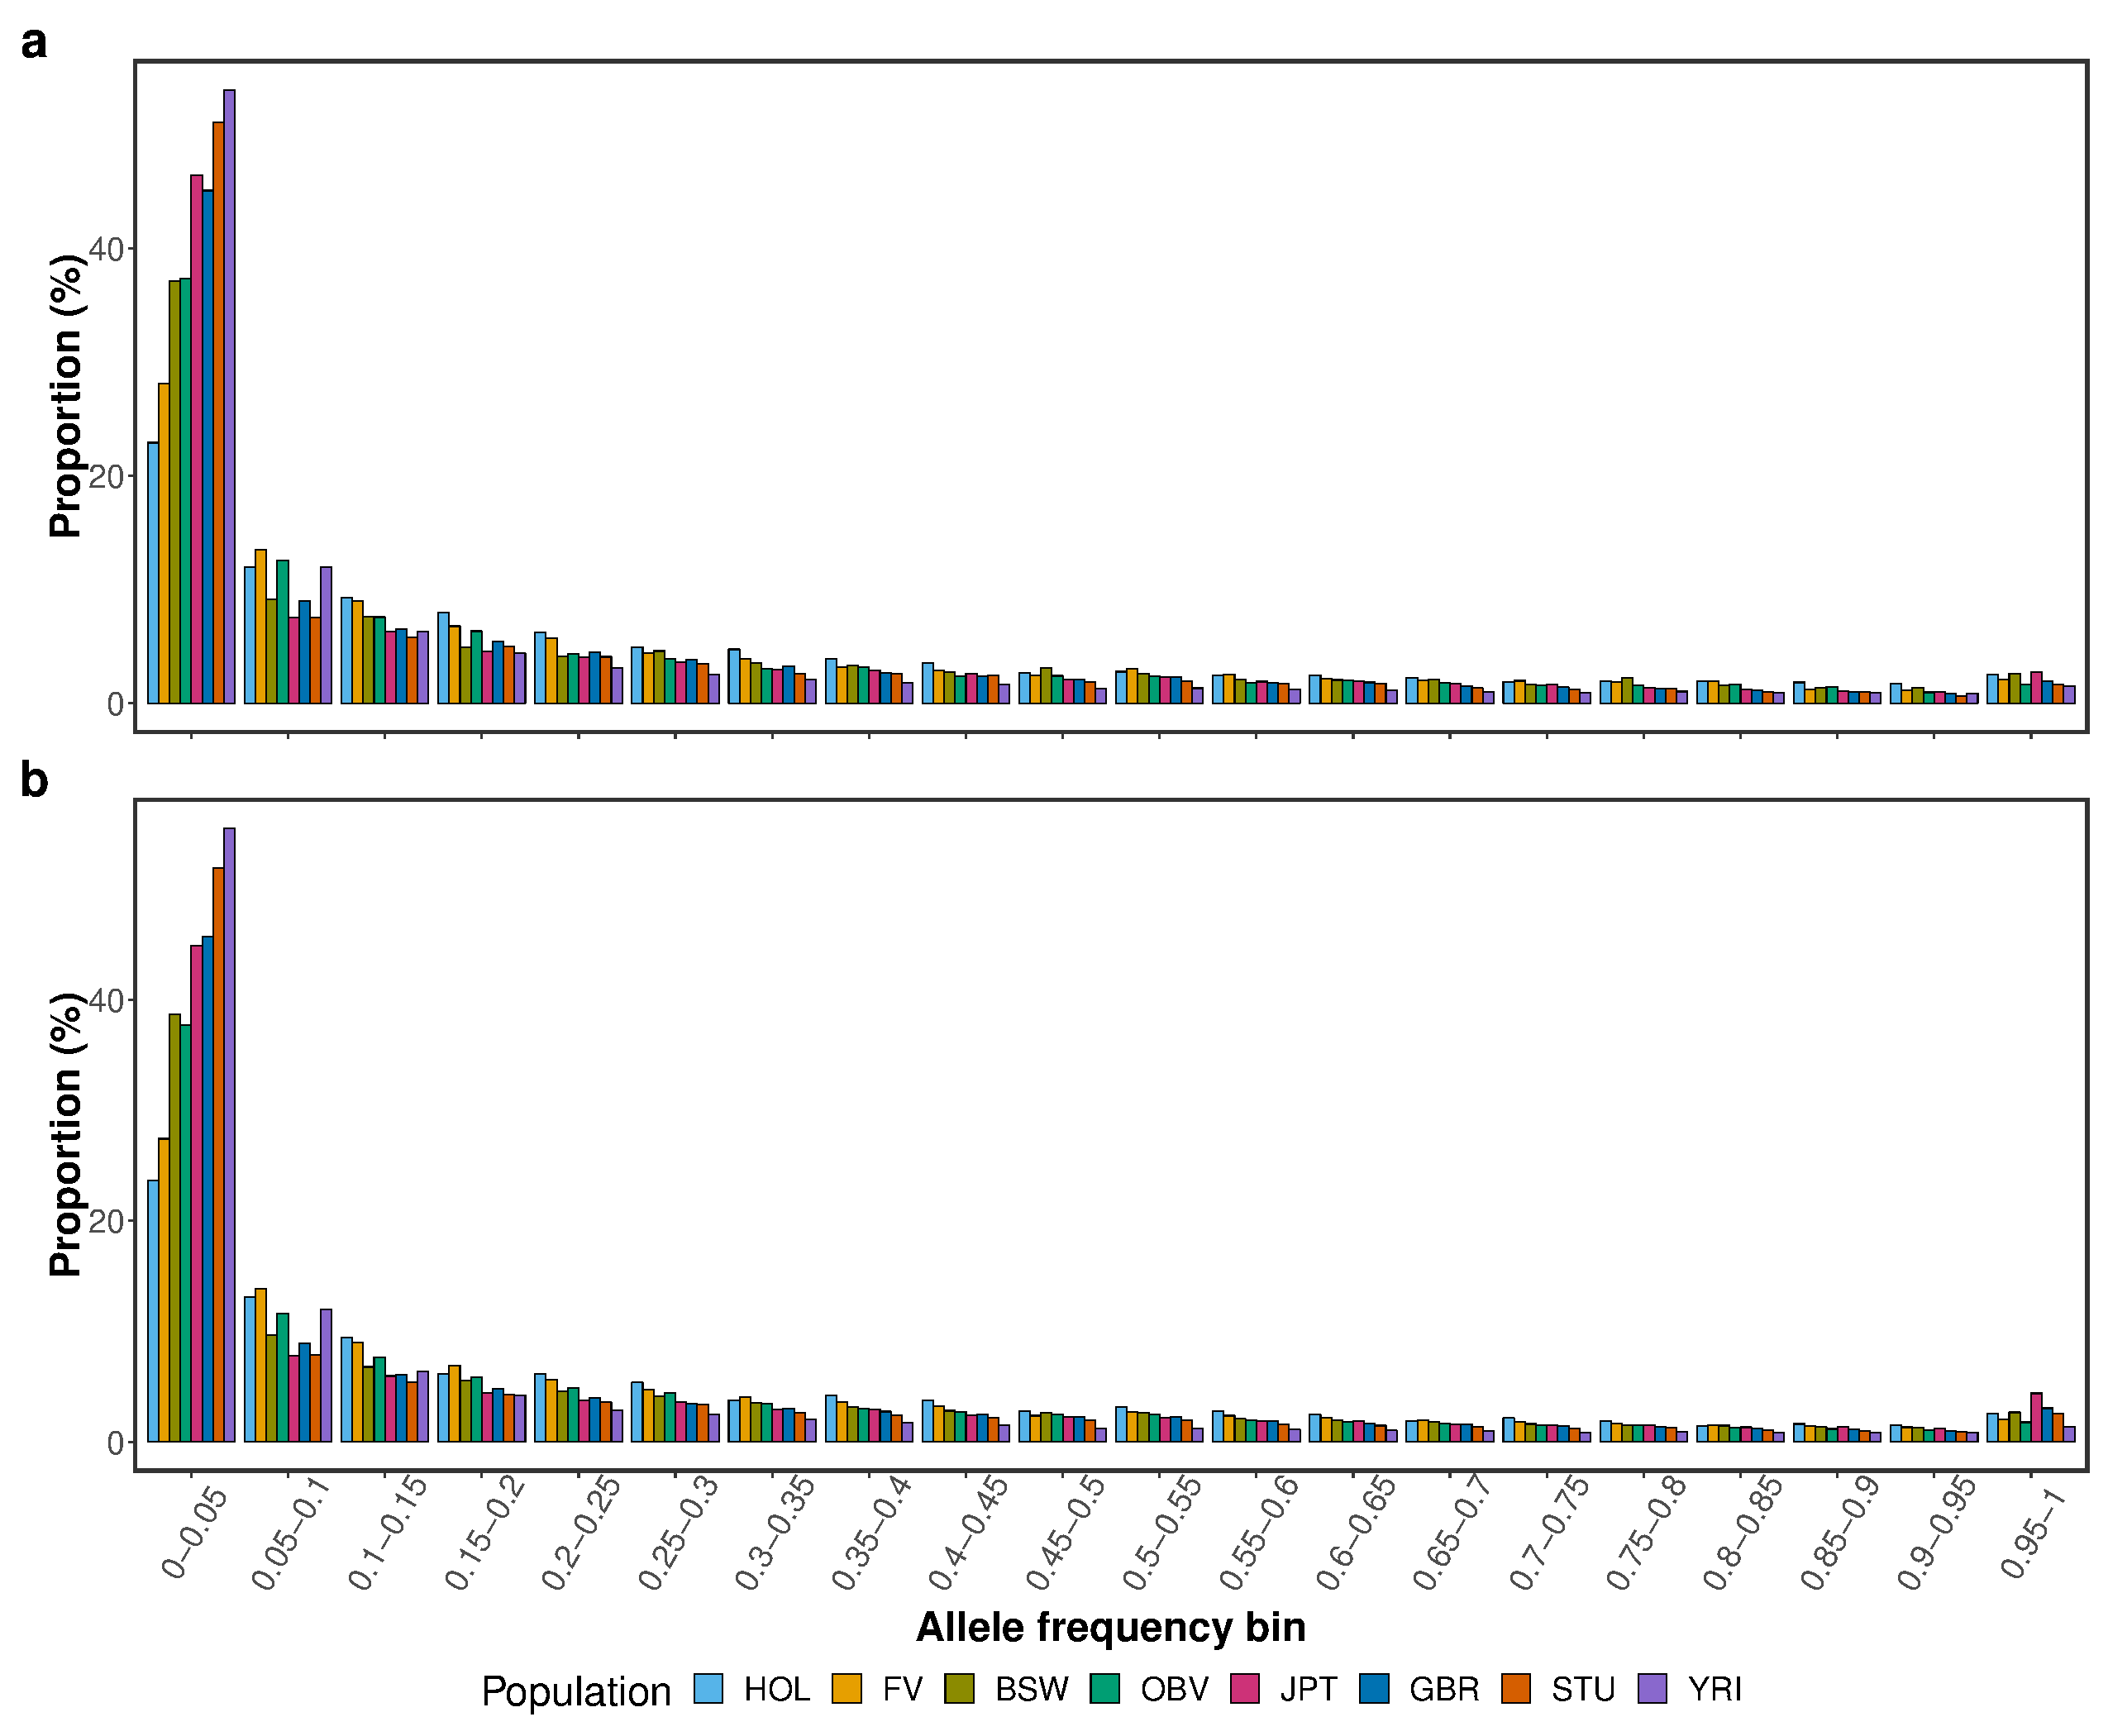
\includegraphics[width=\textwidth]{paper2/supplement/sp34.pdf}
    \caption[Distribution of alternate allele frequencies]{\textbf{Distribution of alternate allele frequencies in four cattle breeds and
    four human populations based on (a) bta25 and human chromosome 19 used
    for graph construction, and (b) whole genome variants. } \\
    \small{The bars indicate the proportion of sequence variants for 20 allele frequency
    classes. Different colour indicates cattle breeds (HOL, FV, BSW, OBV) and human
    populations (JPT, GBR, STU, YRI).}}
    \label{sup_fig:s34}
\end{figure}

\newpage


\begin{figure}[!htb]
    \centering
    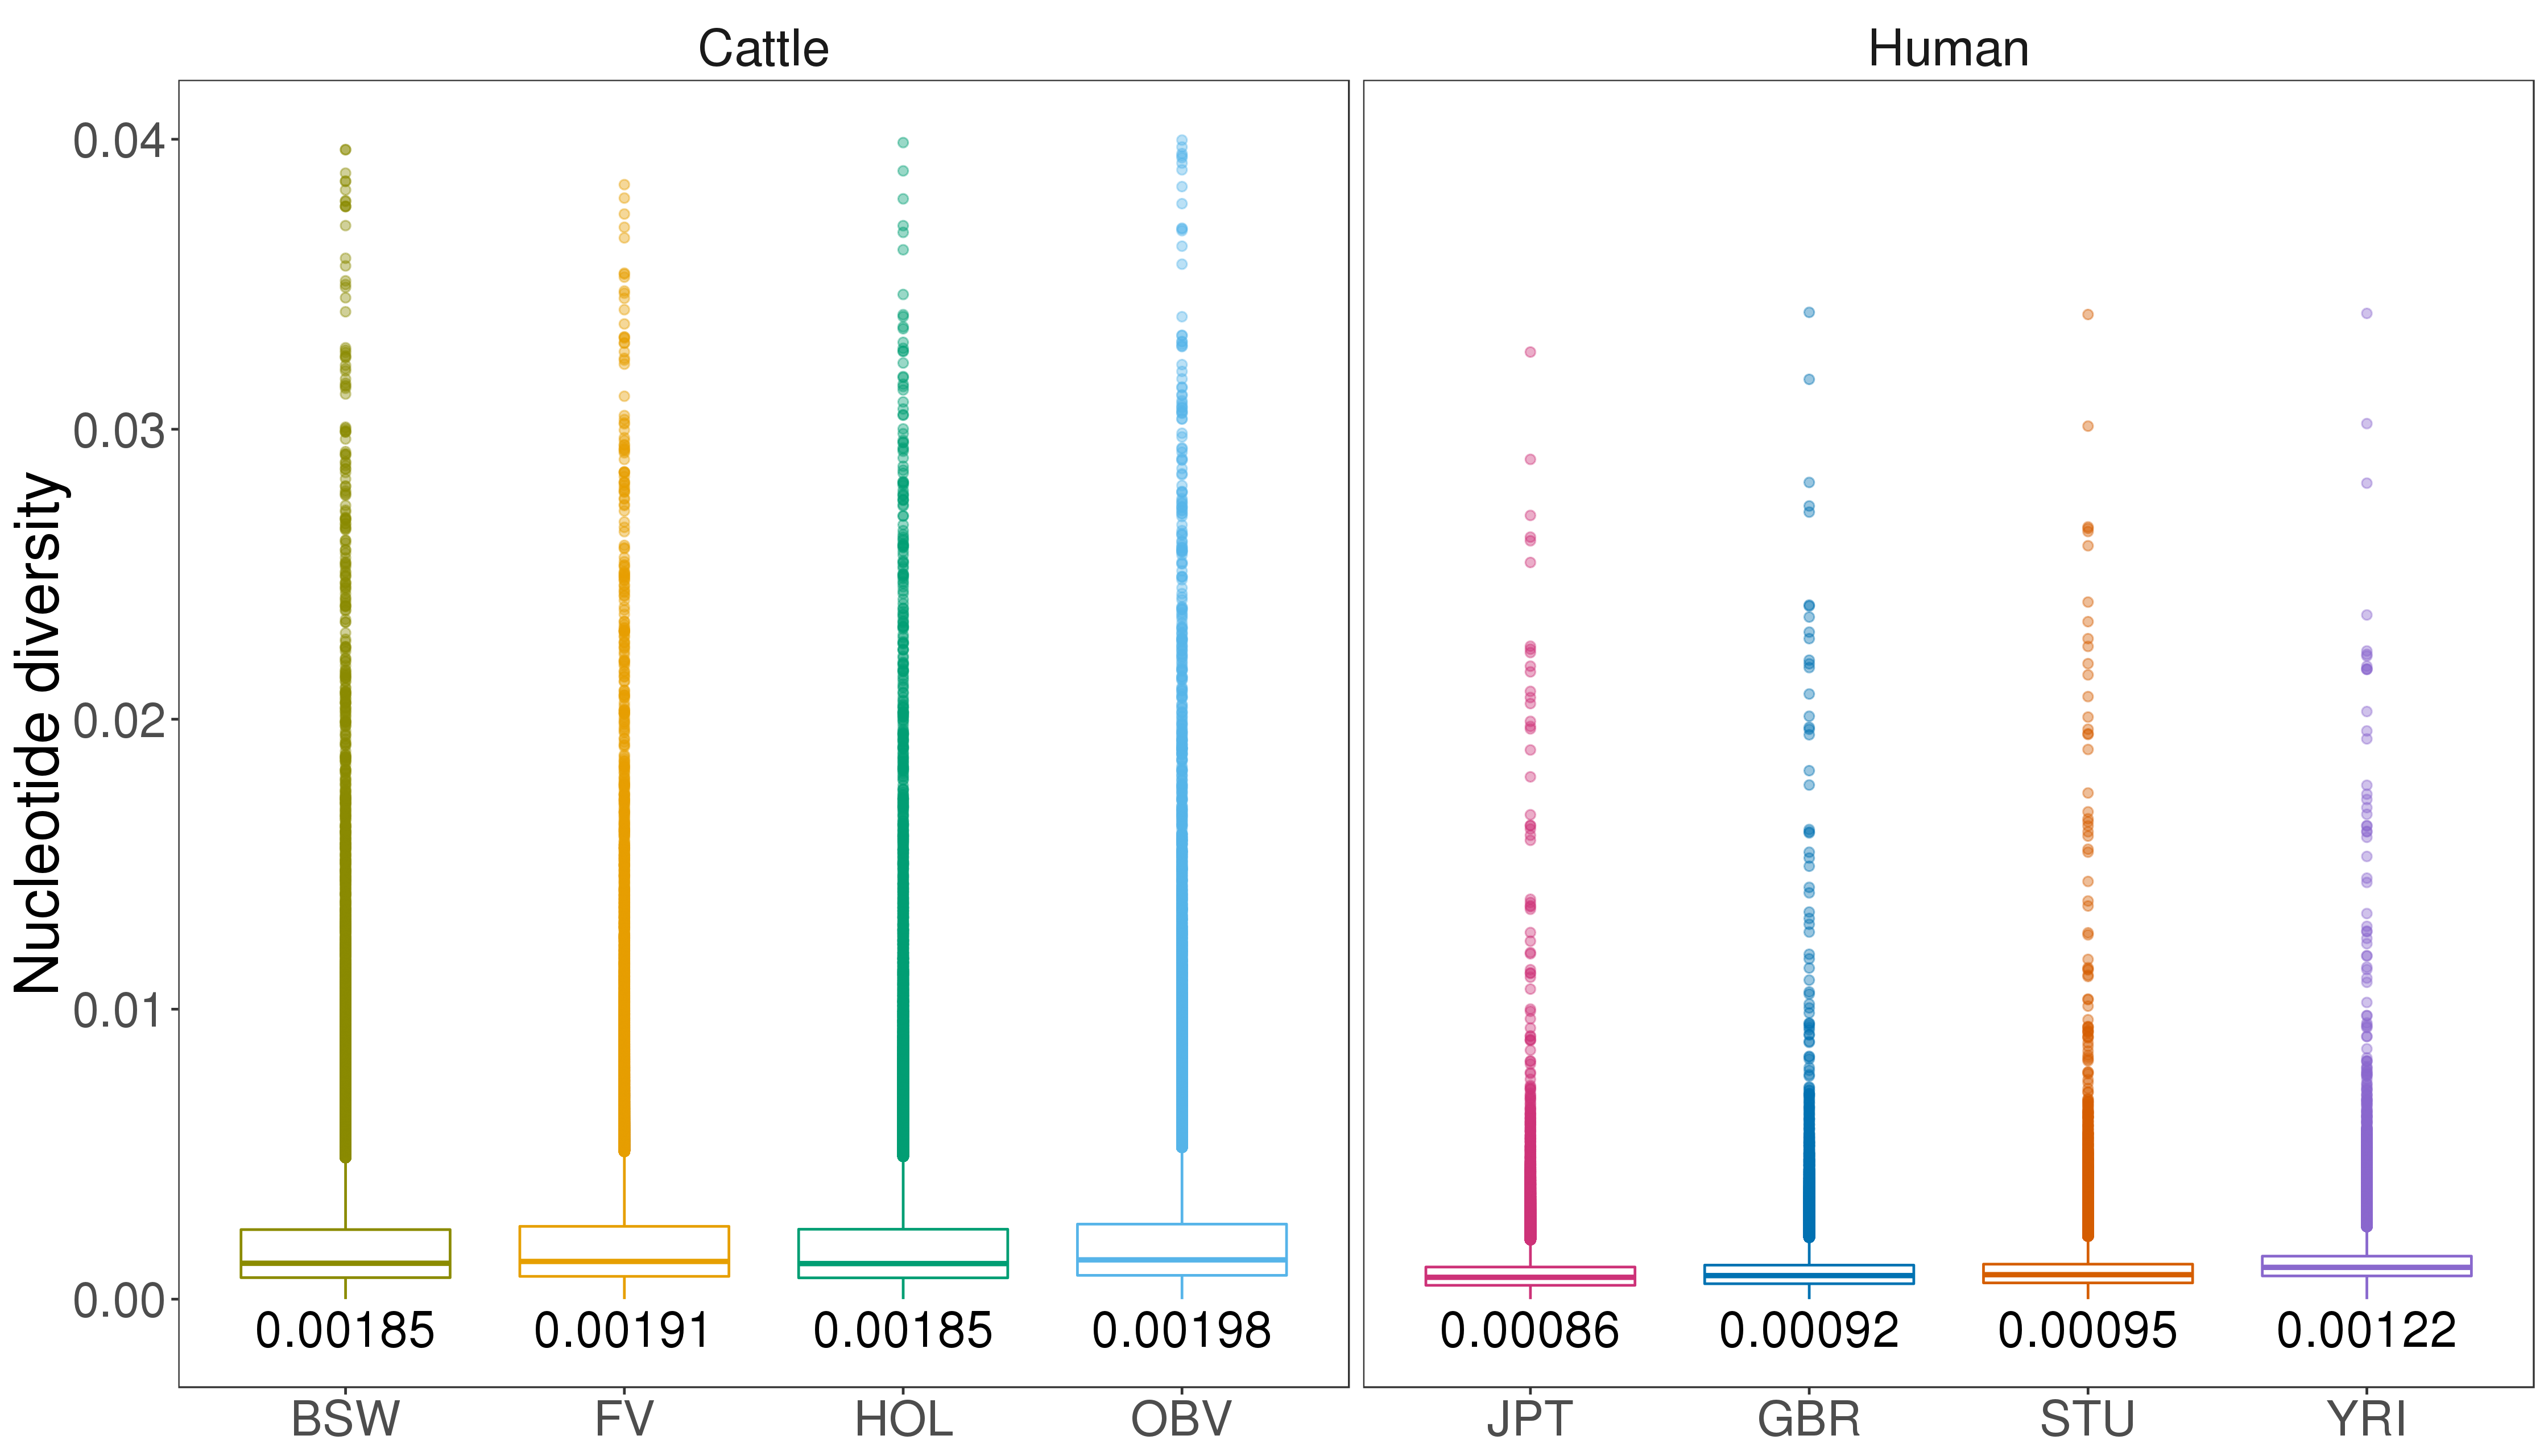
\includegraphics[width=\textwidth]{paper2/supplement/sp35.png}
    \caption[Nucleotide diversity ($\pi$) ]{\textbf{Nucleotide diversity ($\pi$) based on whole genome autosomal variants
    in cattle and human. } \\
    \small{Nucleotide diversity ($\pi$) from each population calculated using vcftools with 10 kb
    non-overlapped windows based on whole genome autosomal variants. Number
    under the boxplot indicates average across windows.}}
    \label{sup_fig:s35}
\end{figure}

\begin{figure}[!htb]
    \centering
    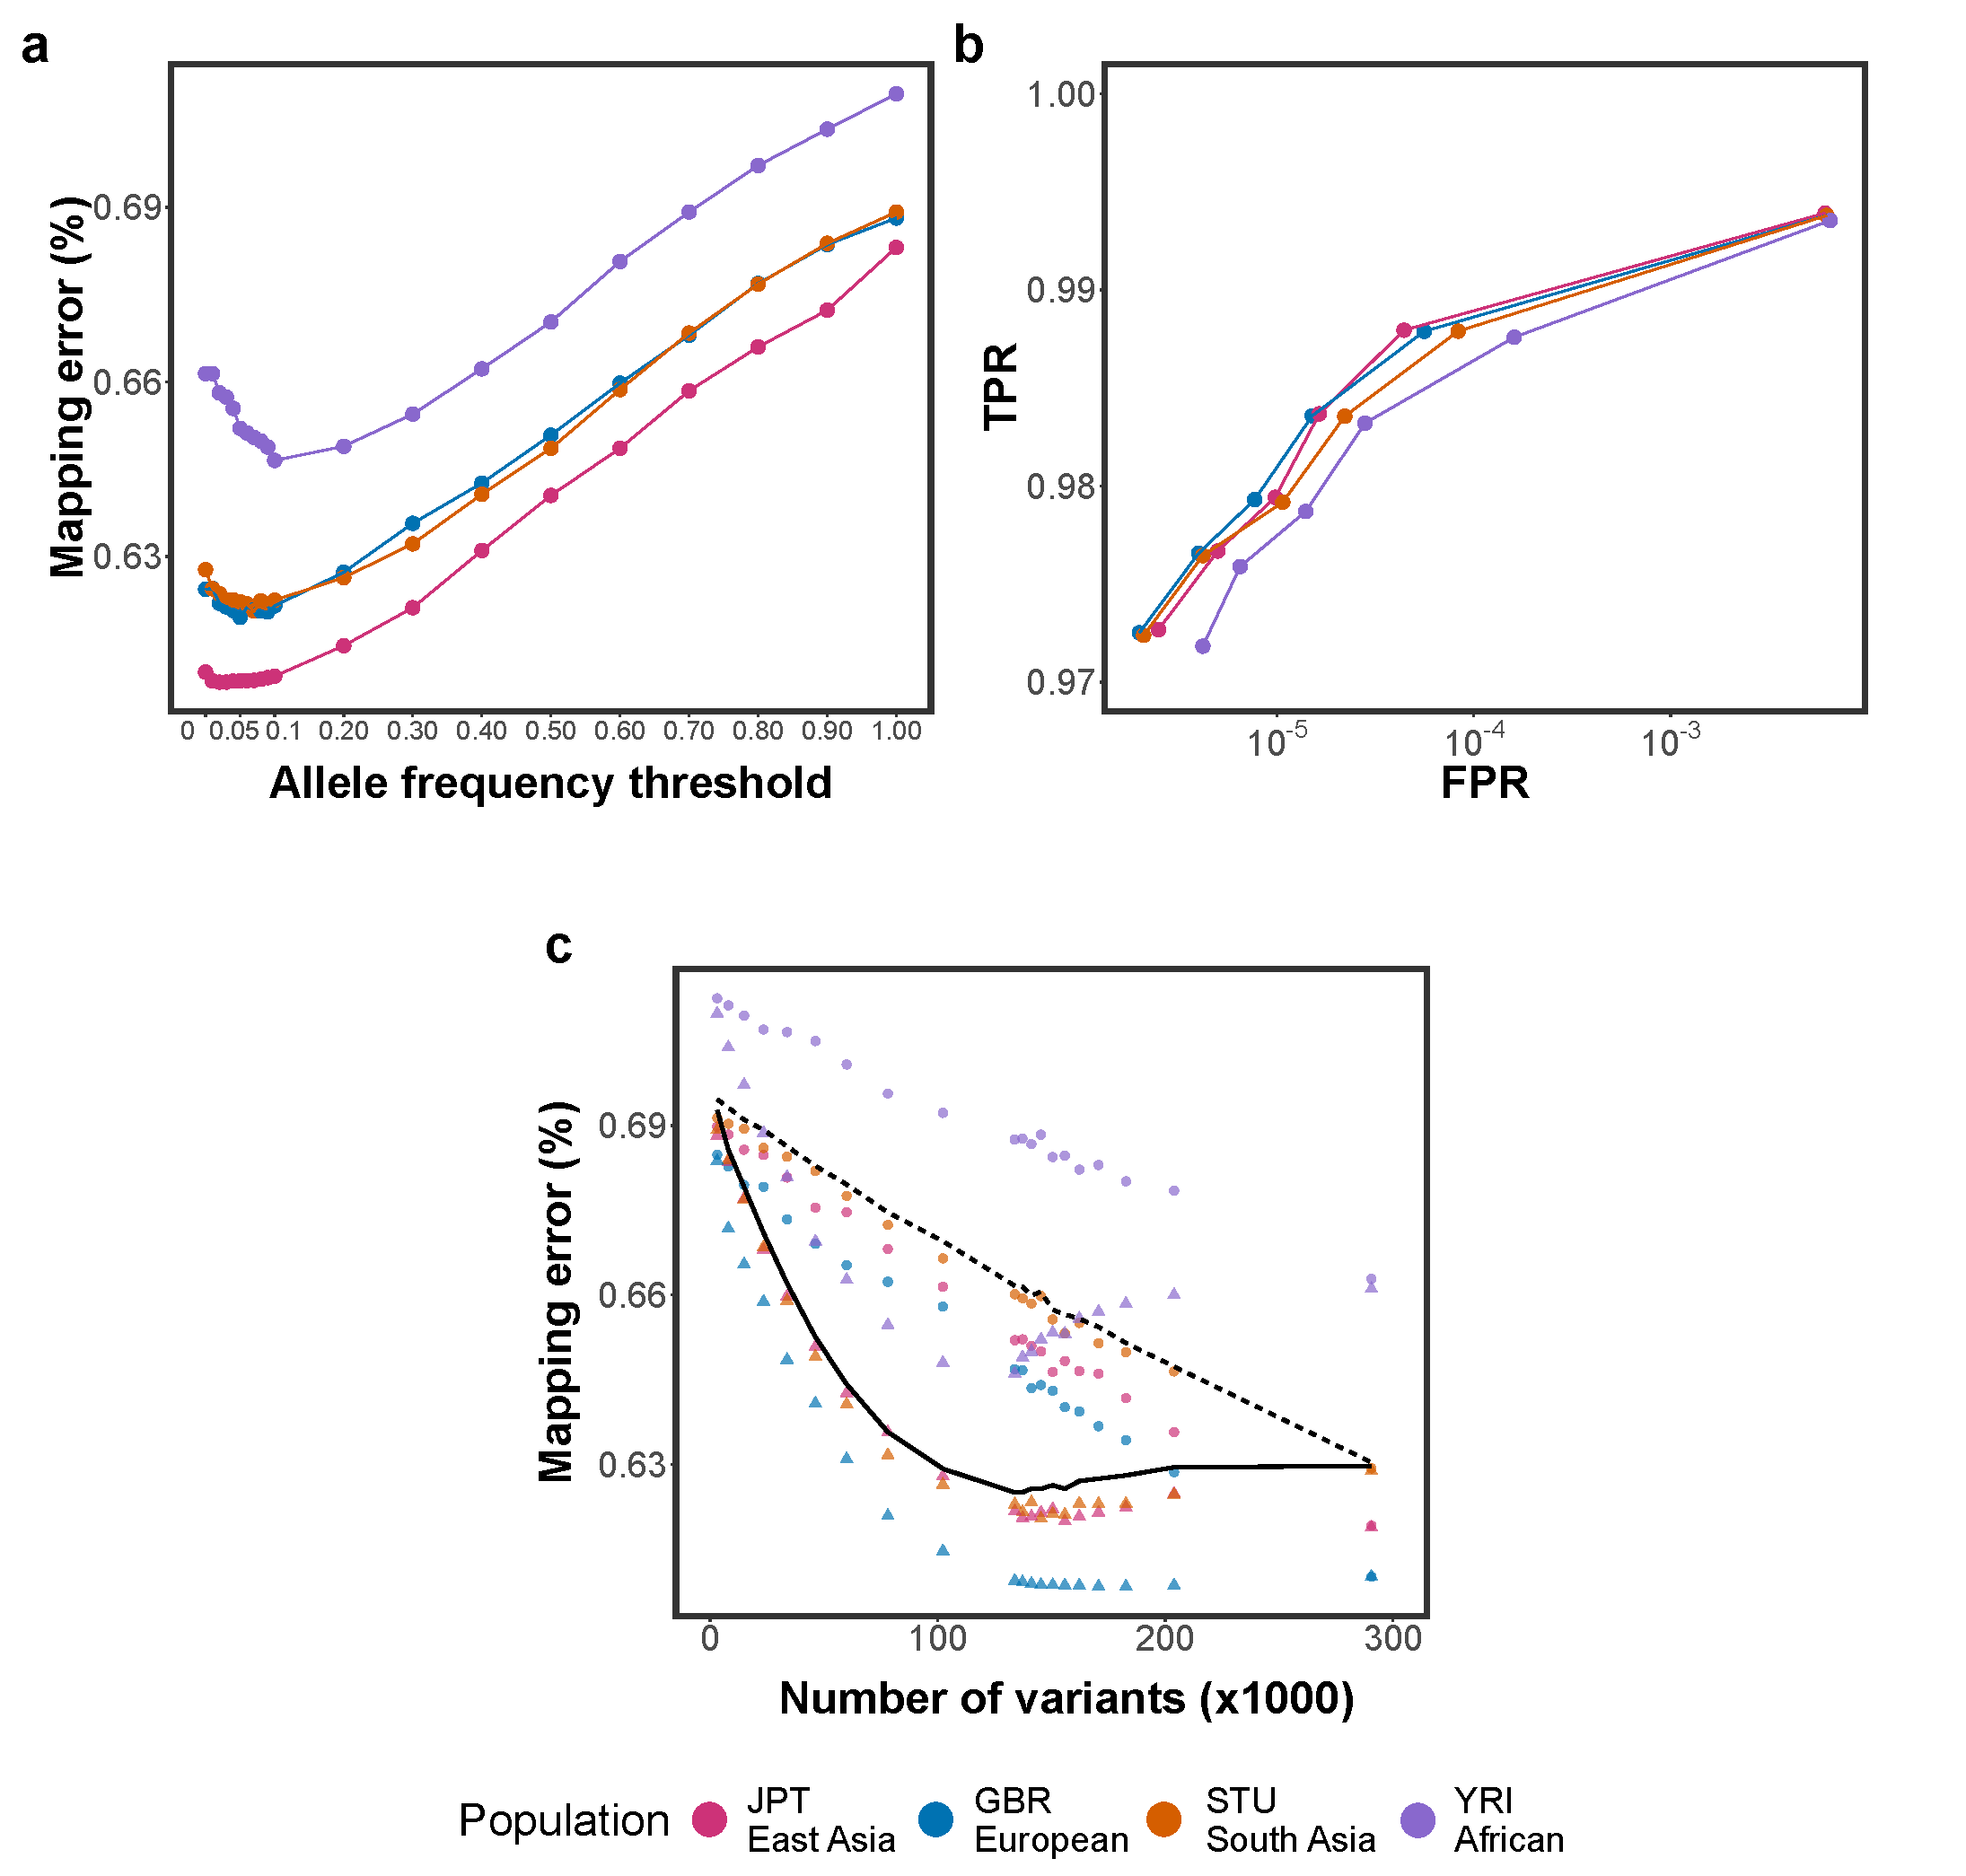
\includegraphics[width=\textwidth]{paper2/supplement/sp36.pdf}
    \caption[Single mapping accuracy using human graphs]{\textbf{Single-end mapping accuracy using four human population-specific
    augmented graphs. } \\
    \small{(a) Proportion of incorrectly mapped reads for four populationspecific augmented genome graphs (b) True positive (sensitivity) and false positive
    mapping rate (specificity) parameterized based on the mapping quality for the best
    performing graph from each population. (c) Read mapping accuracy for population specific augmented graphs that contained variants that were either filtered for
    alternate allele frequency (triangles) or sampled randomly (circles) from all variants detected within a population. The dashed and solid line represents the average proportion of mapping errors across four populations using variant prioritization and random sampling.}}
    \label{sup_fig:s36}
\end{figure}

\begin{figure}[!htb]
    \centering
    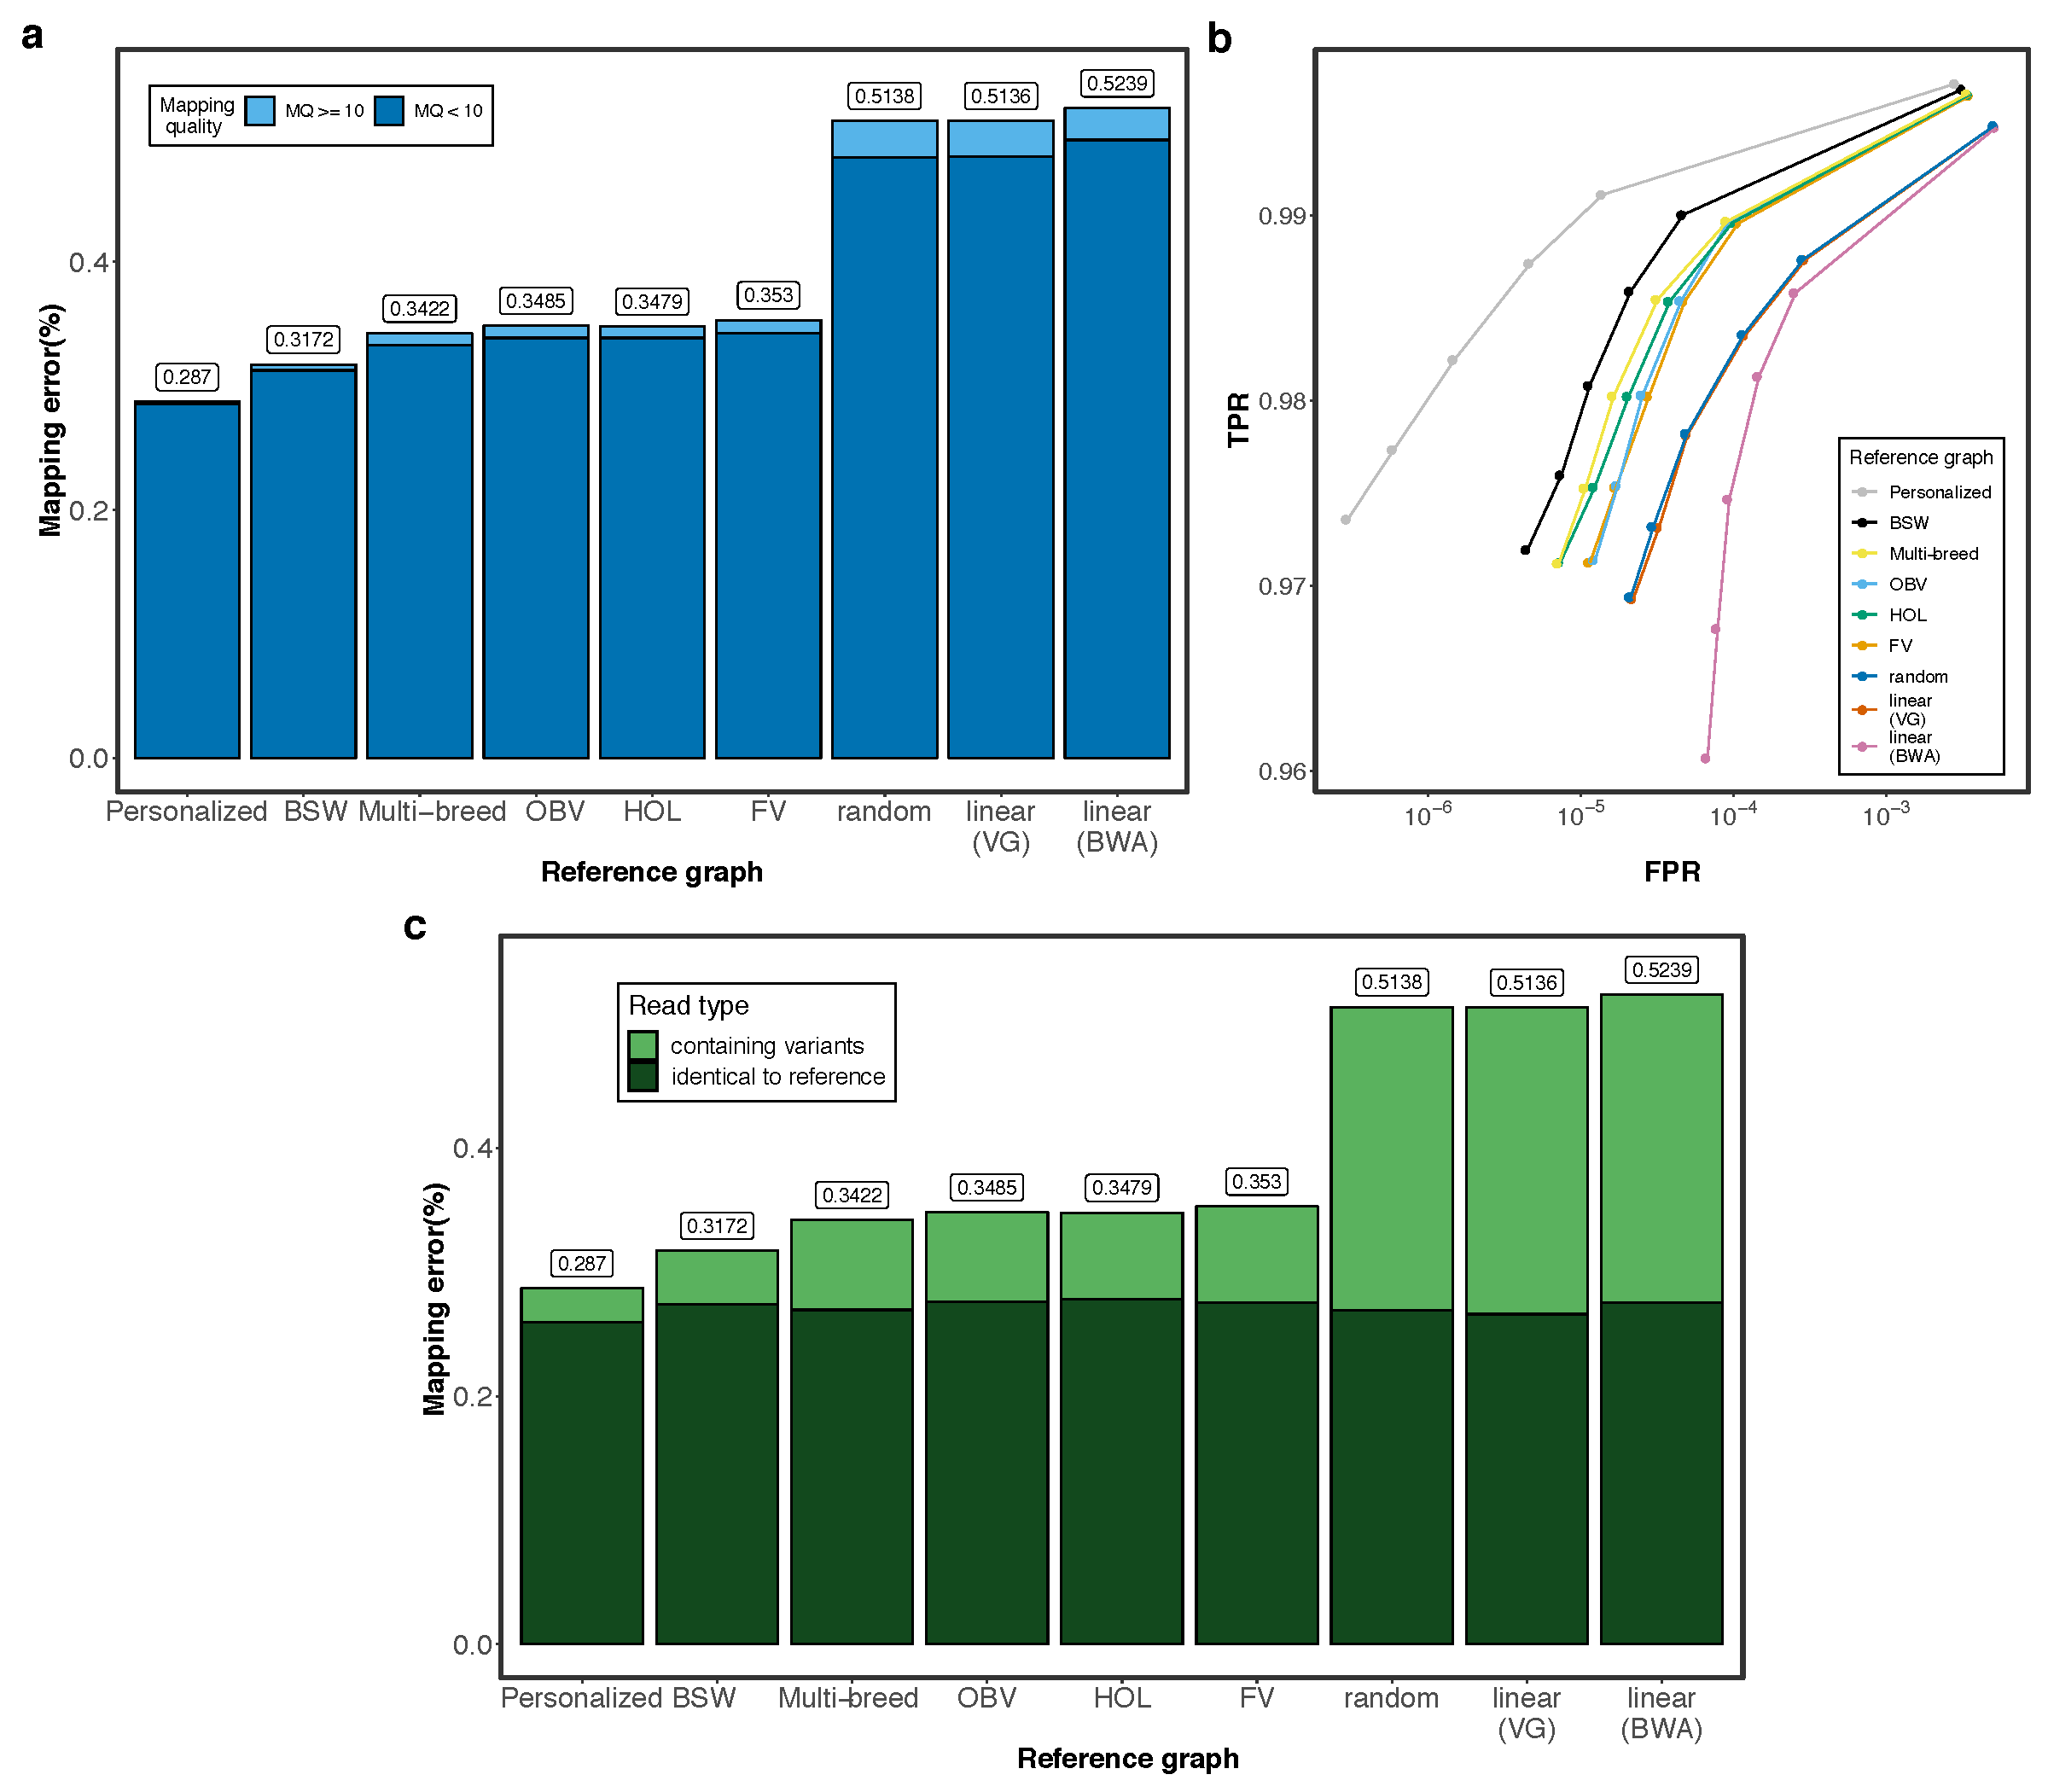
\includegraphics[width=\textwidth]{paper2/supplement/sp37.pdf}
    \caption[The accuracy of mapping simulated BSW single-end reads]{\textbf{The accuracy of mapping simulated BSW single-end reads to
    variation-aware and linear reference structures.} \\
    \small{(a) Proportion of BSW single-end reads that mapped erroneously against breed-specific
    augmented graphs, random graphs or linear reference sequences. Dark and light blue
    colours represent the proportion of incorrectly mapped reads with mapping quality (MQ)$<$10
    and MQ$>$10, respectively. (b) True positive (sensitivity) and false positive mapping rate
    (specificity) parameterized based on the mapping quality. (c) Dark and light green colours
    represent the proportion of incorrectly mapped reads that matched corresponding reference
    nucleotides and contained non-reference alleles, respectively}}
    \label{sup_fig:s37}
\end{figure}


\begin{figure}[!htb]
    \centering
    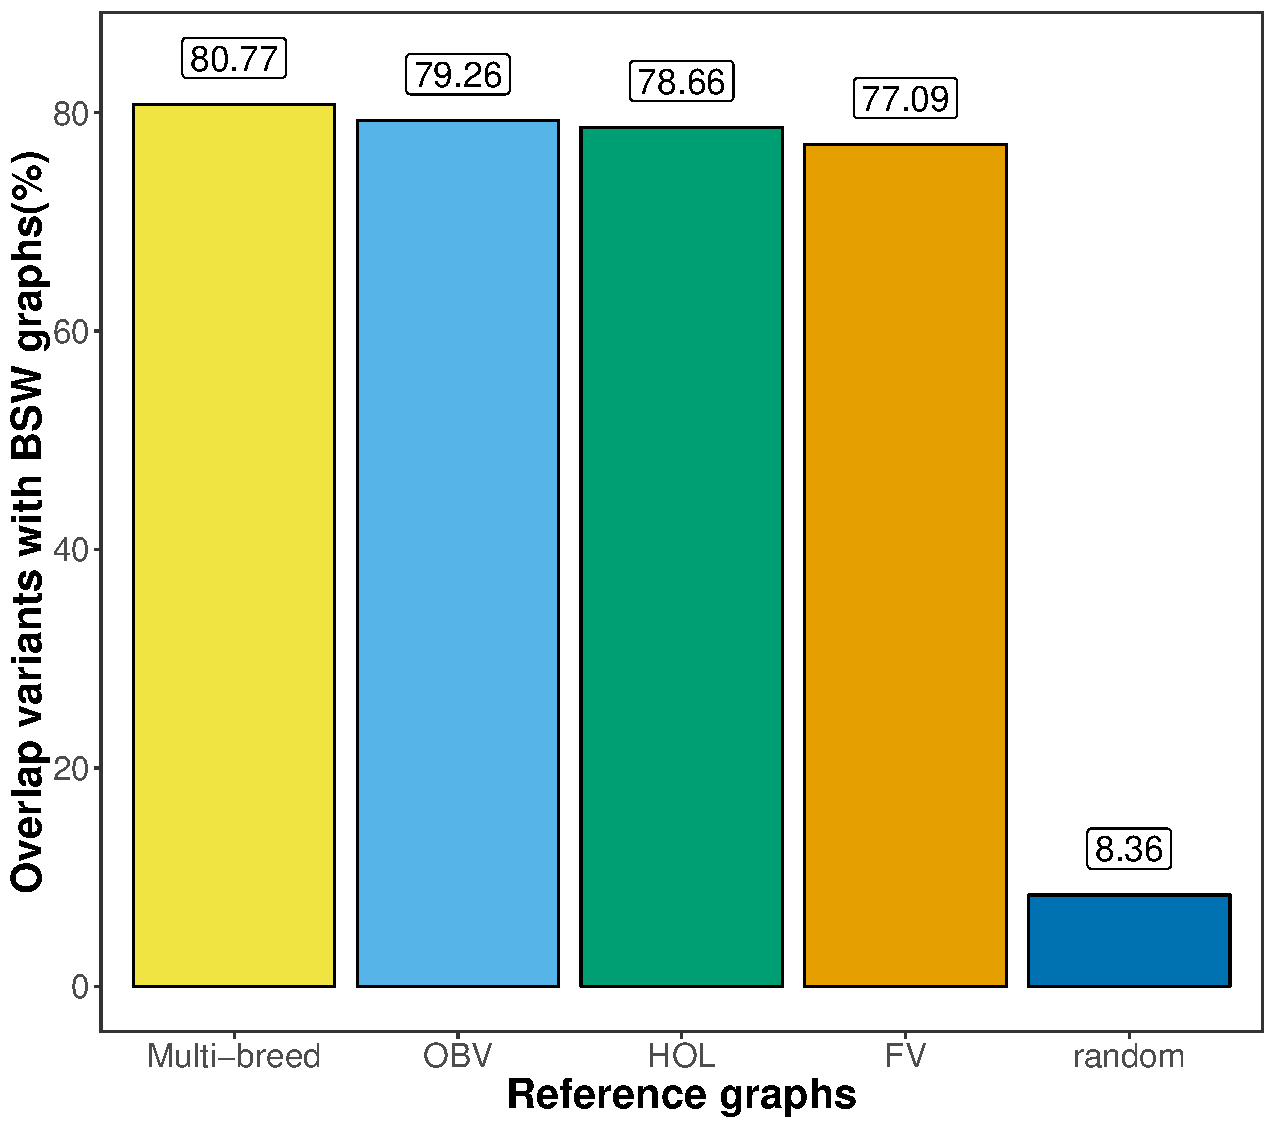
\includegraphics[width=\textwidth]{paper2/supplement/sp38.pdf}
    \caption[Overlap of the variants]{\textbf{Overlap of the variants} \\
    \small{(N=243,145) between the BSW-and all other
    variation-aware reference graphs. The values are averaged across 10 replicates.}}
    \label{sup_fig:s38}
\end{figure}

\begin{figure}[!htb]
    \centering
    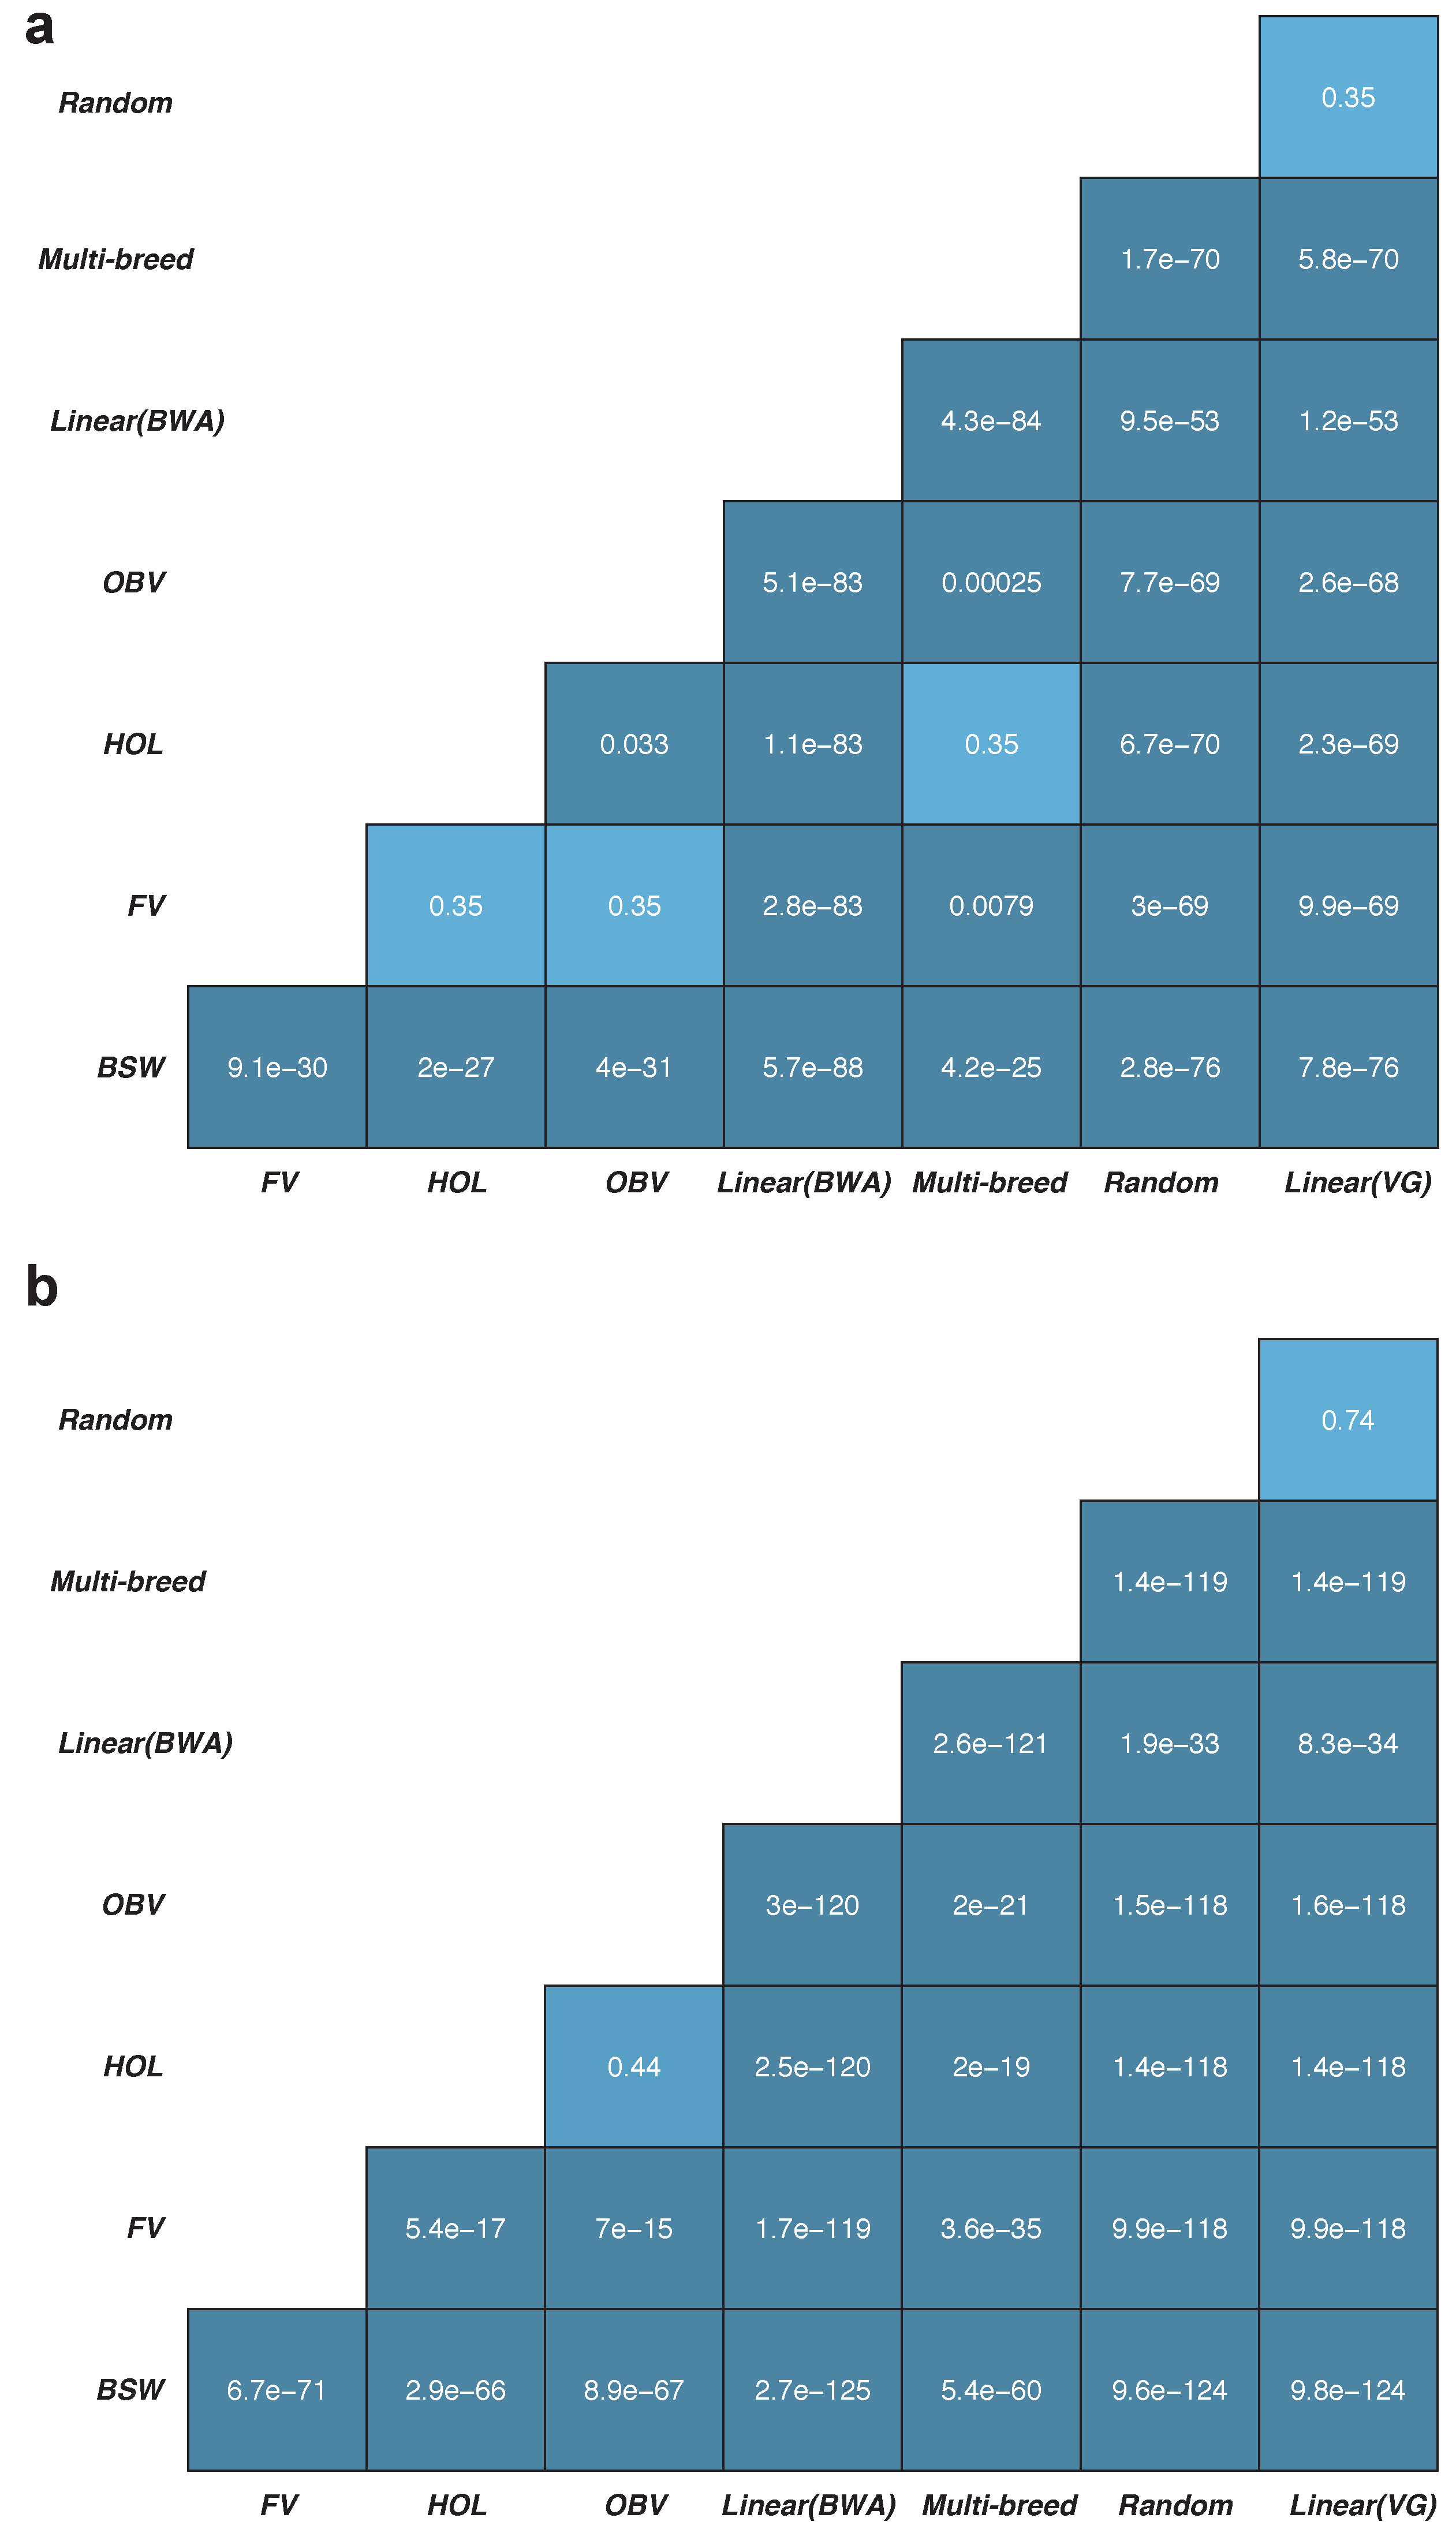
\includegraphics[width=0.7\textwidth]{paper2/supplement/sp39.pdf}
    \caption[Pairwise heatmap of 8 graphs comparison]{\textbf{Pairwise heatmap of \emph{P-values} from \emph{t tests}} \\
    \small{comparing 8 graph-based
    mapping scenarios for (a) paired- and (b) single-end reads. The P-values are
    adjusted for multiple testing using Bonferroni-correction.}}
    \label{sup_fig:s39}
\end{figure}

\begin{figure}[!htb]
    \centering
    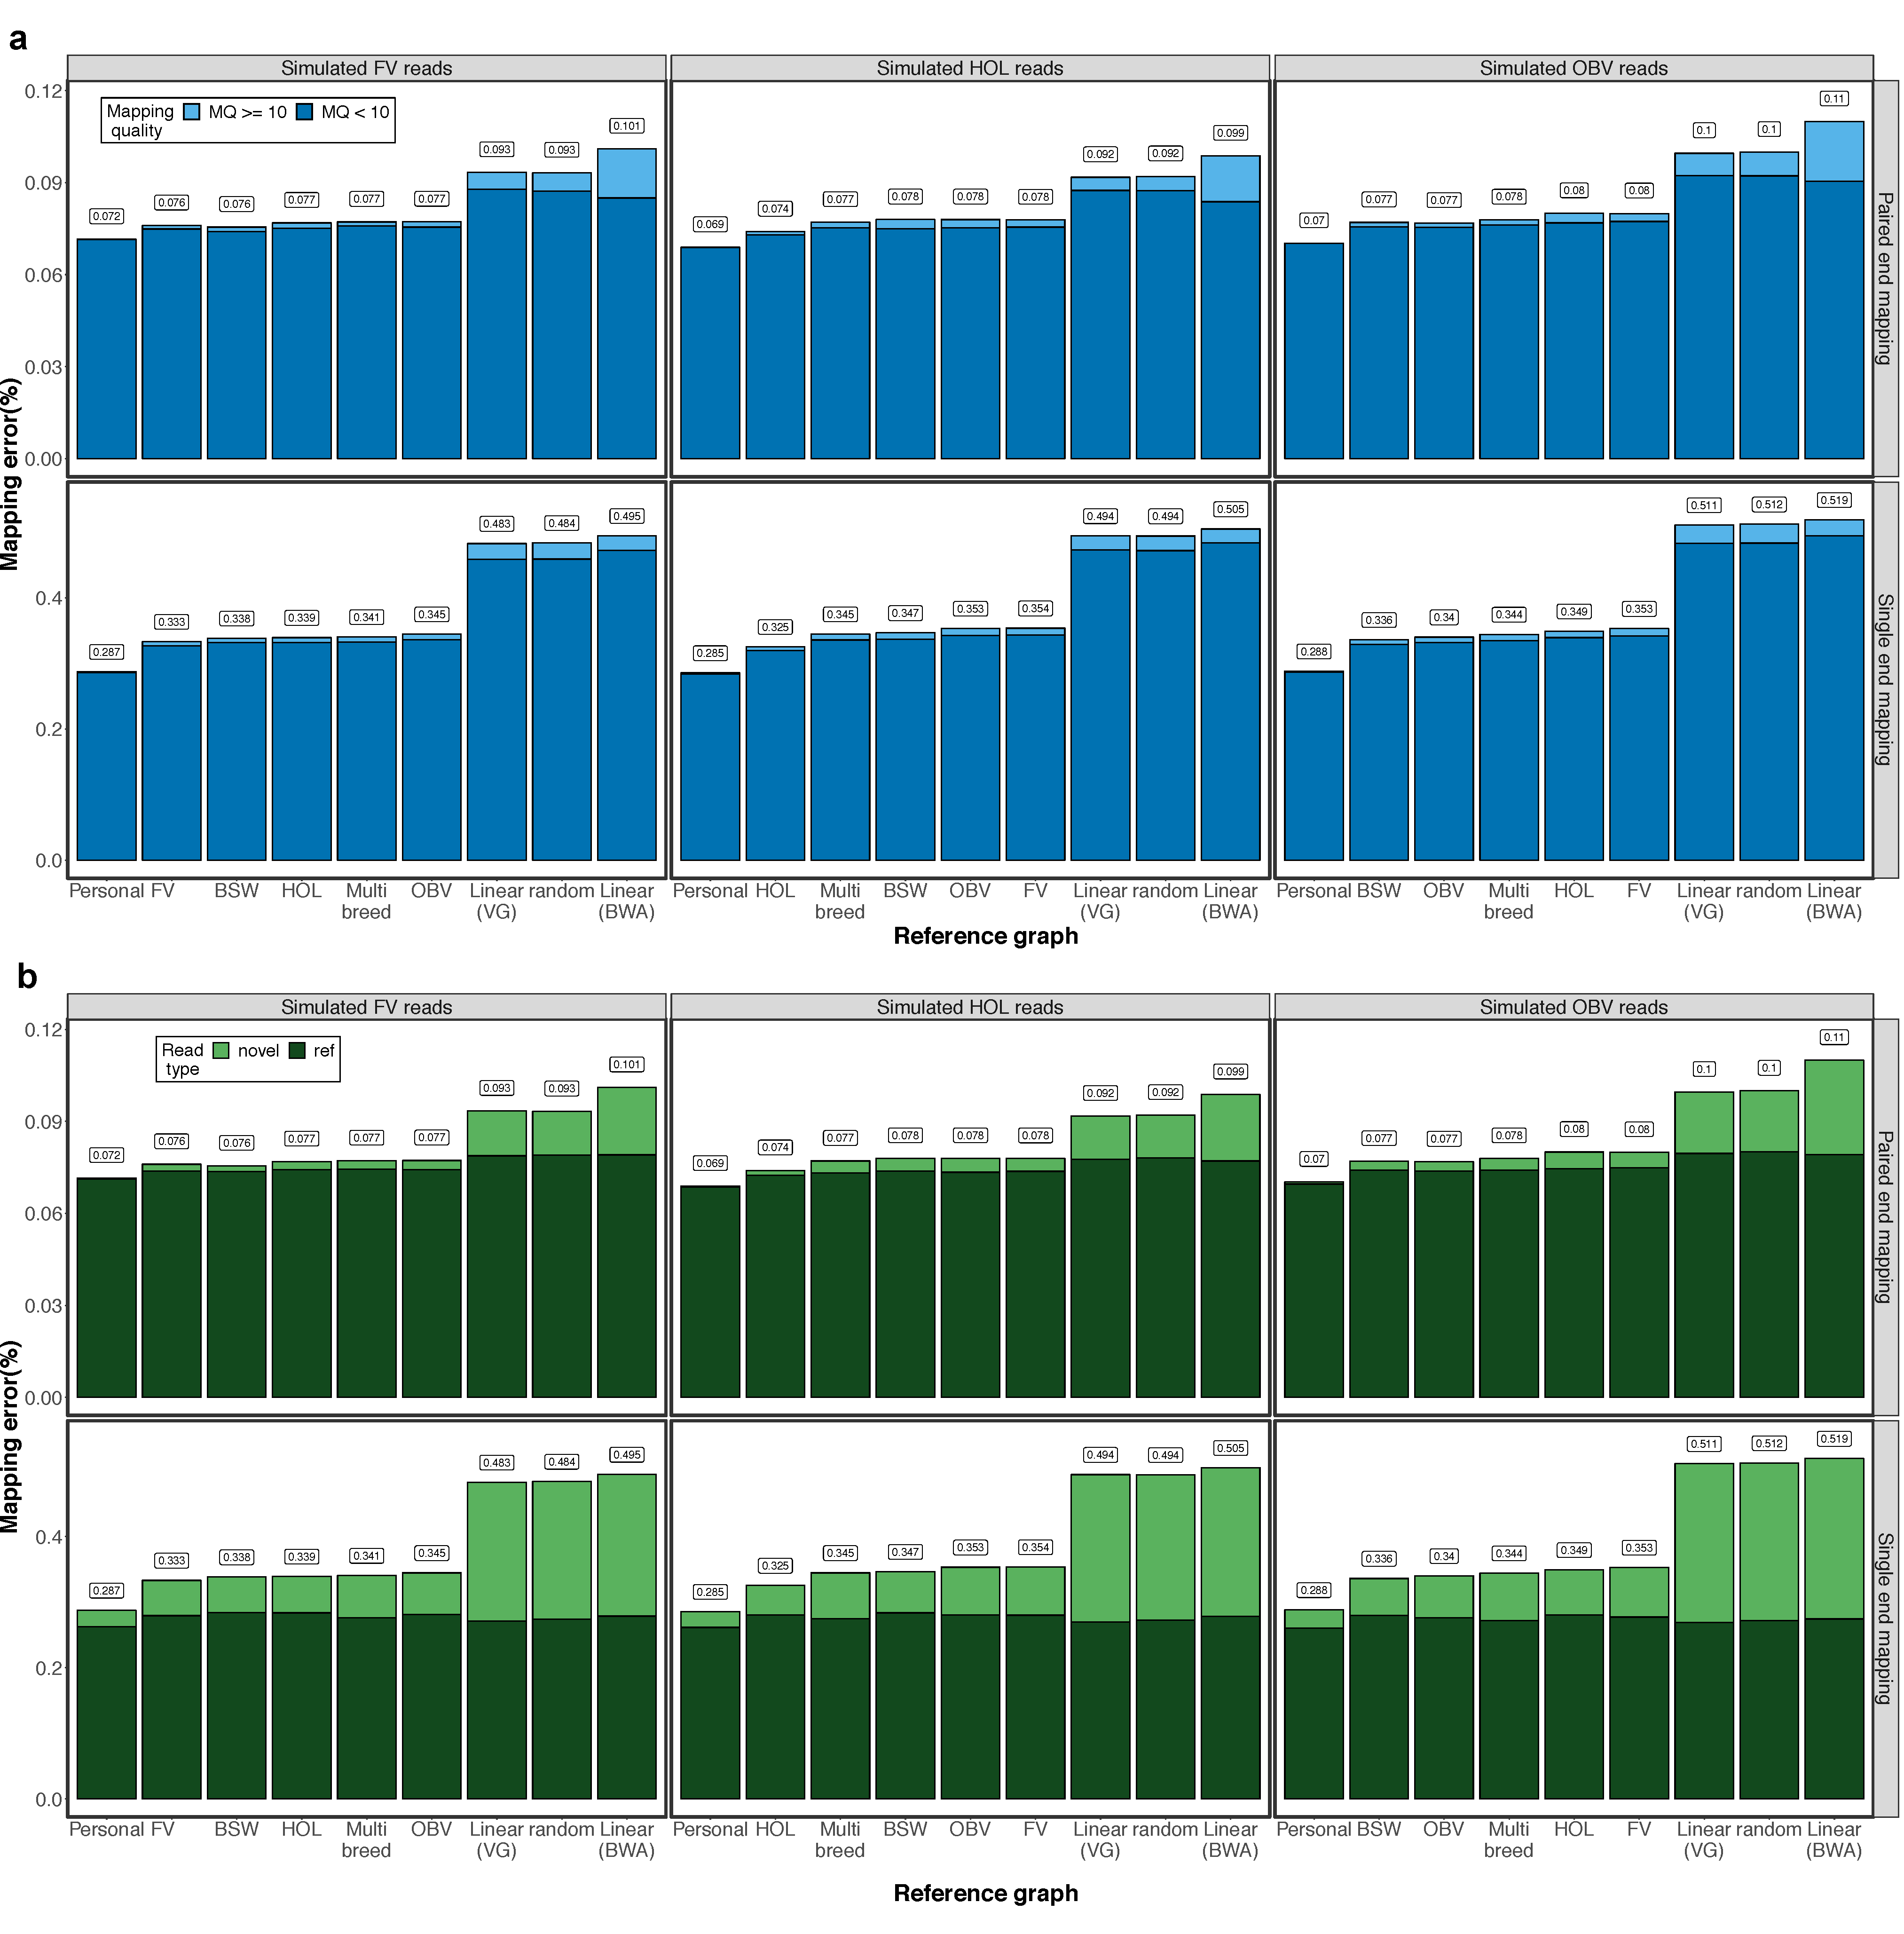
\includegraphics[width=\textwidth]{paper2/supplement/sp310.pdf}
    \caption[The accuracy of mapping simulated FV, HOL and OBV reads]{\textbf{The accuracy of mapping simulated FV, HOL and OBV reads to
    variation-aware and linear reference structures.} \\
    \small{(a) Proportion of reads that
    mapped erroneously against personalized graphs, breed-specific augmented graphs,
    random graphs or linear reference sequences. Dark and light blue colours represent
    the proportion of incorrectly mapped reads with mapping quality (MQ)$<$10 and
    MQ$>$10, respectively. The upper and lower panels reflect paired-end and single-end
    reads, respectively. (b) Dark and light green colours represent the proportion of
    incorrectly mapped reads that matched corresponding reference nucleotides and
    contained non-reference alleles, respectively. The upper and lower panels reflect
    paired-end and single-end reads, respectively}}
    \label{sup_fig:s310}
\end{figure}

\begin{figure}[!htb]
    \centering
    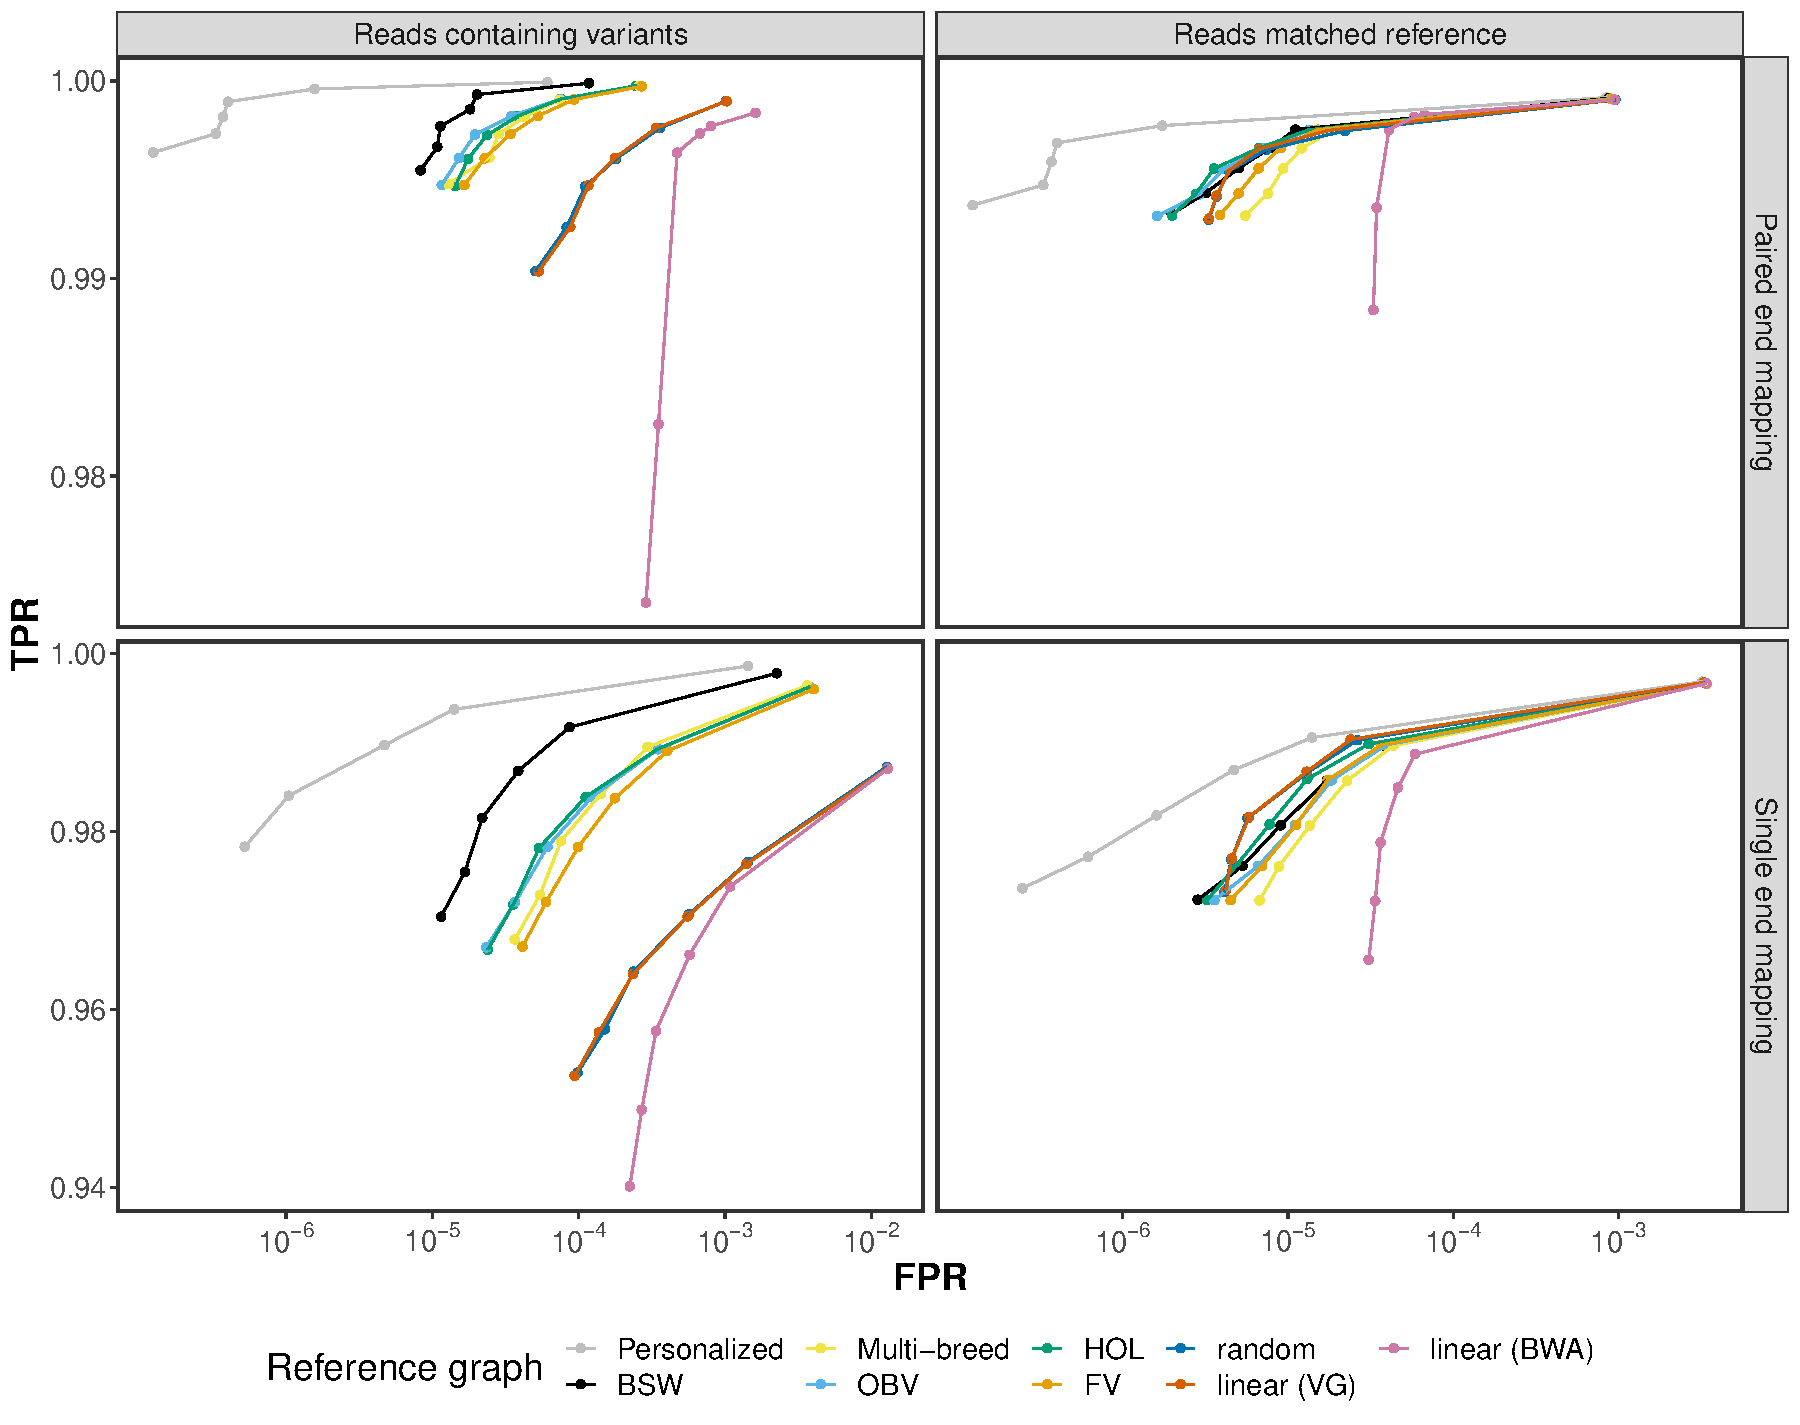
\includegraphics[width=\textwidth]{paper2/supplement/sp311.pdf}
    \caption[ ROC curves split by read’s novelty]{\textbf{ROC curves split by read’s novelty} \\
    \small{Cumulative \emph{True positive} and \emph{False positive rate} at different mapping quality
    thresholds visualized as Receiver Operating Characteristic (ROC) curves for reads
    than contain variants and match corresponding reference alleles. The upper and
    lower panels represent results from paired- and single-end reads.}}
    \label{sup_fig:s311}
\end{figure}

\begin{figure}[!htb]
    \centering
    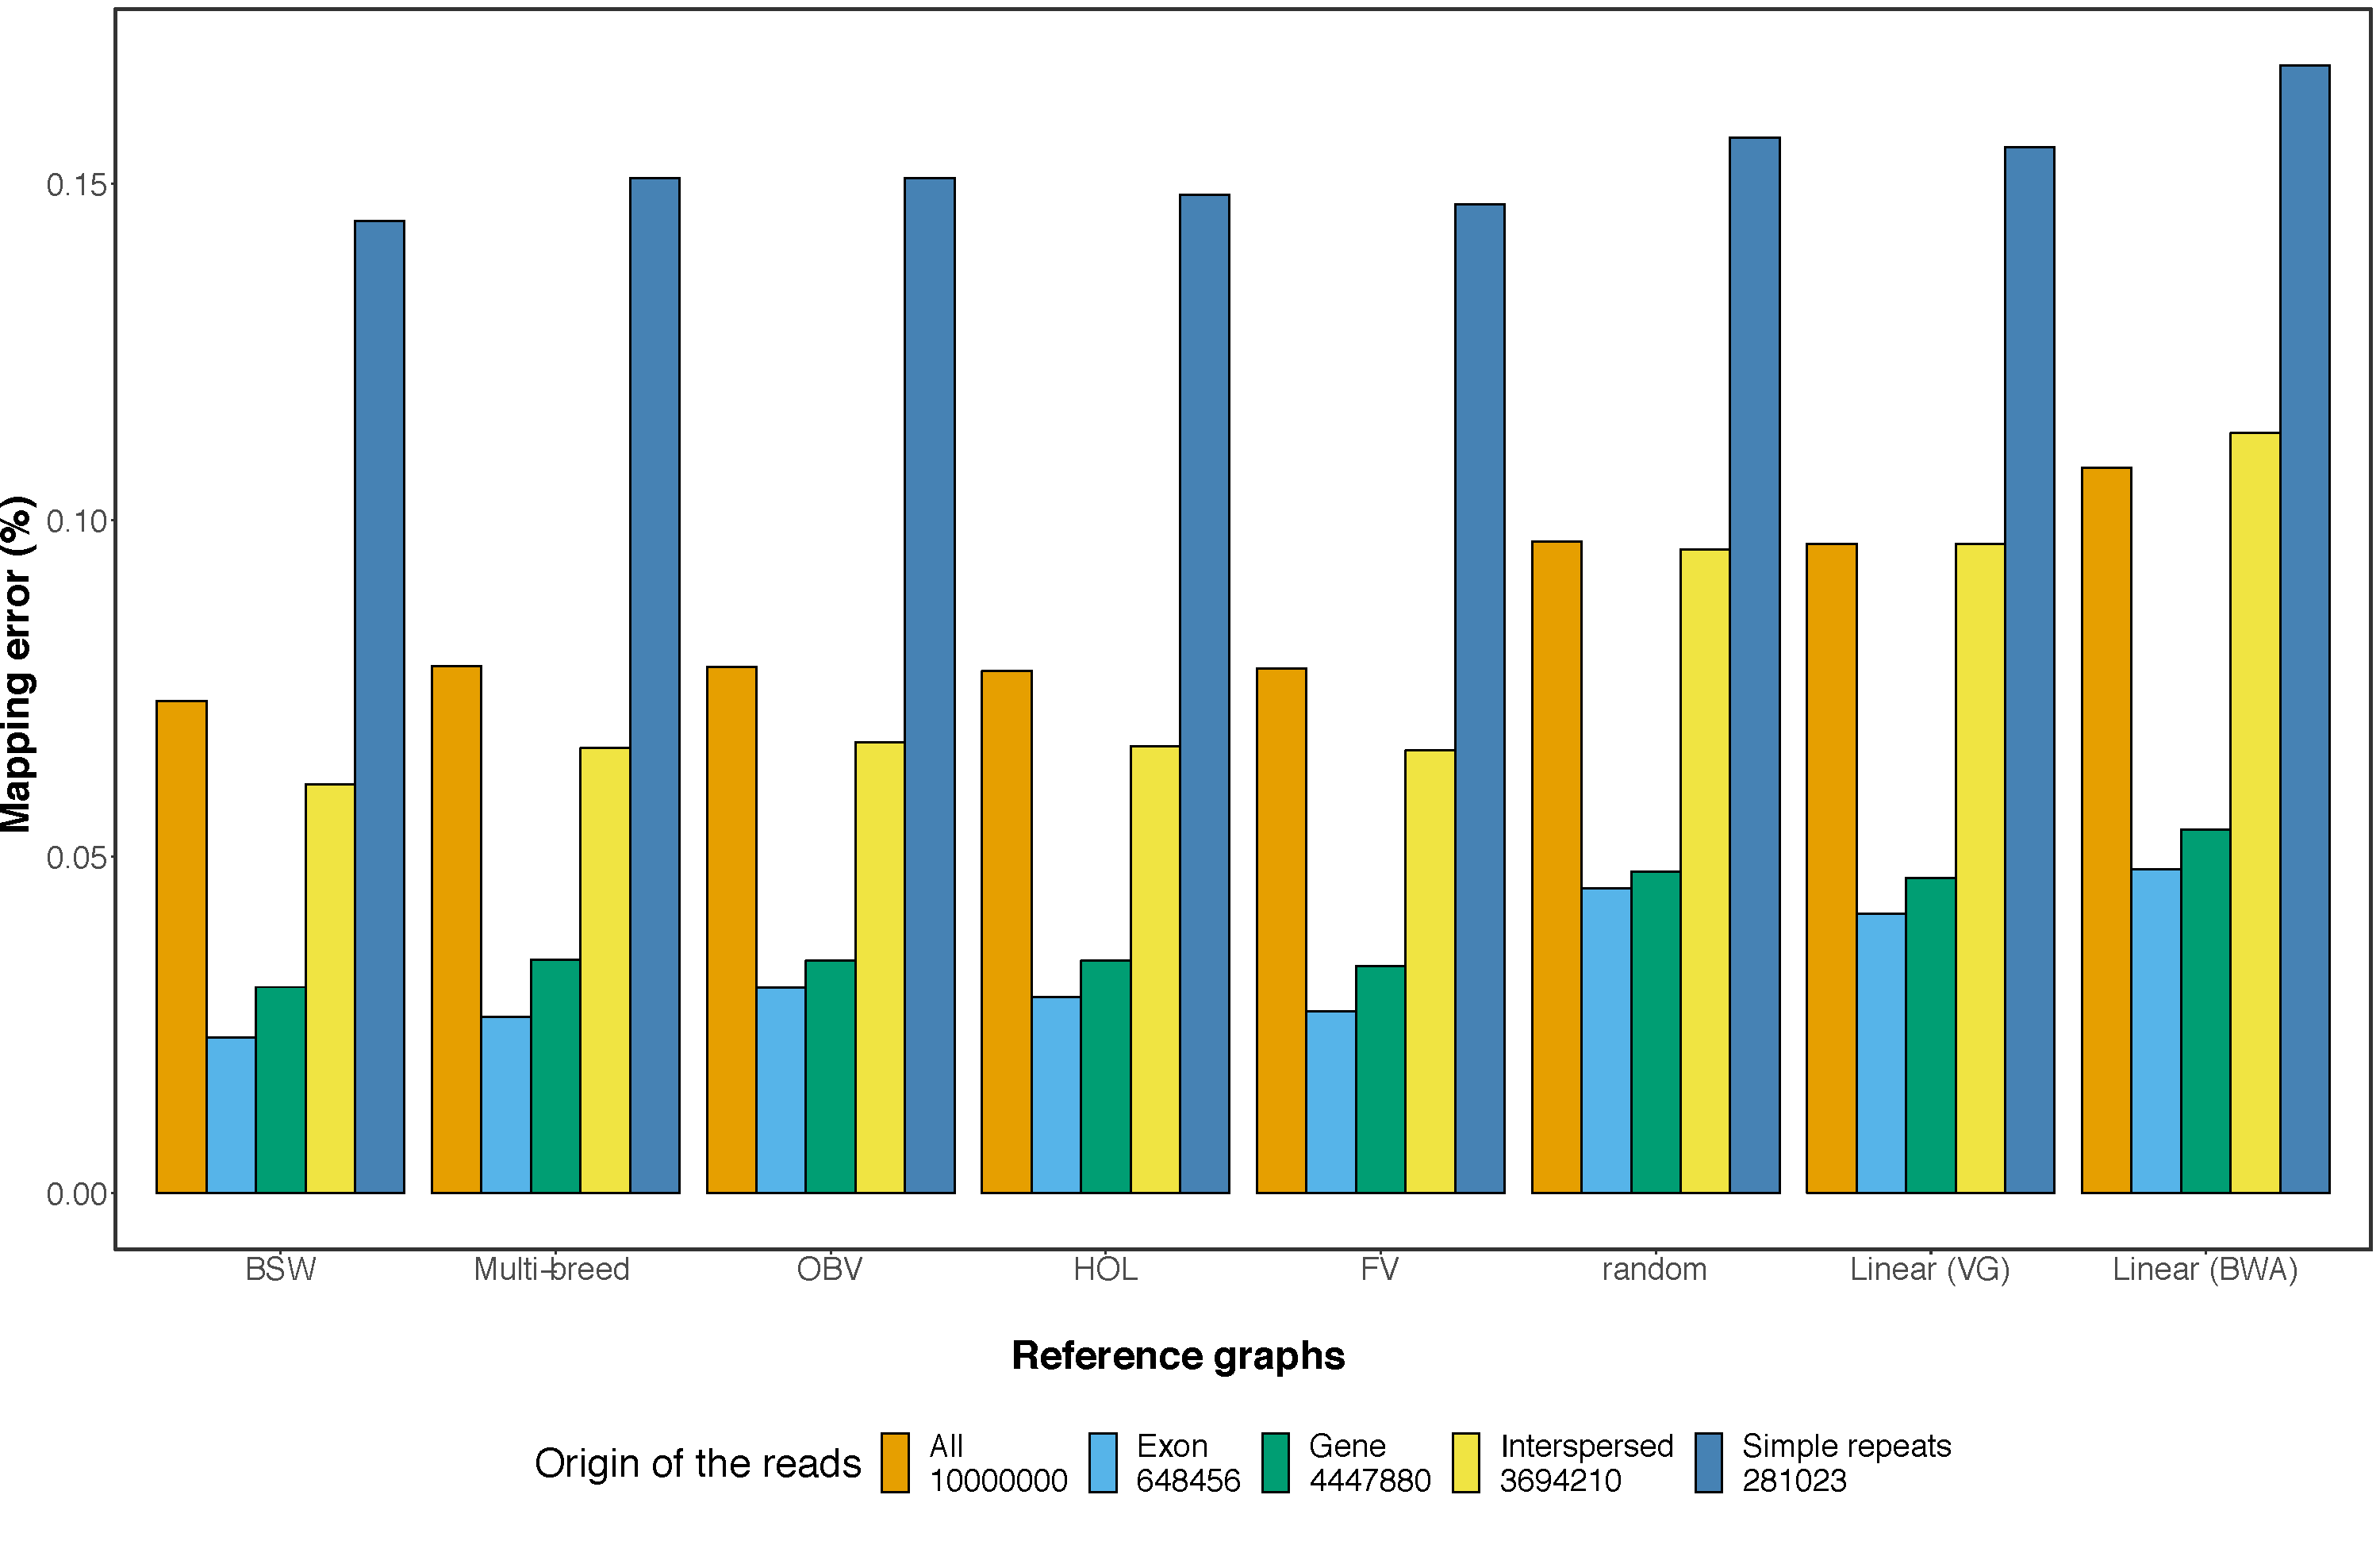
\includegraphics[width=\textwidth]{paper2/supplement/sp312.pdf}
    \caption[ Mapping accuracy from different genomic features.]{\textbf{Mapping accuracy for reads originating from different genomic
    features.} \\
    \small{The origin of 10 million simulated reads was determined based on the Bos taurus
    ARS-UCD1.2 ensembl 99 annotations (exonic and genic) and the ARS-UCD1.2
    repeat regions labelled by Repeat Masker (Interspersed duplications including
    SINEs, LINEs, LTR, and DNA transposable elements, and simple repeats which
    contain low-complexity and simple repetitive regions). Different colour indicates the
    proportion of erroneously mapped reads for each annotation category. The orange
    bars represent the average proportion of mis-mapped reads for six graph-based
    (BSW, Multi-breed, OBV, HOL, FV, random) and two linear (VG, BWA) reference
    structures. Reads were simulated from haplotypes of a BSW individual.}}
    \label{sup_fig:s312}
\end{figure}


\begin{figure}[!htb]
    \centering
    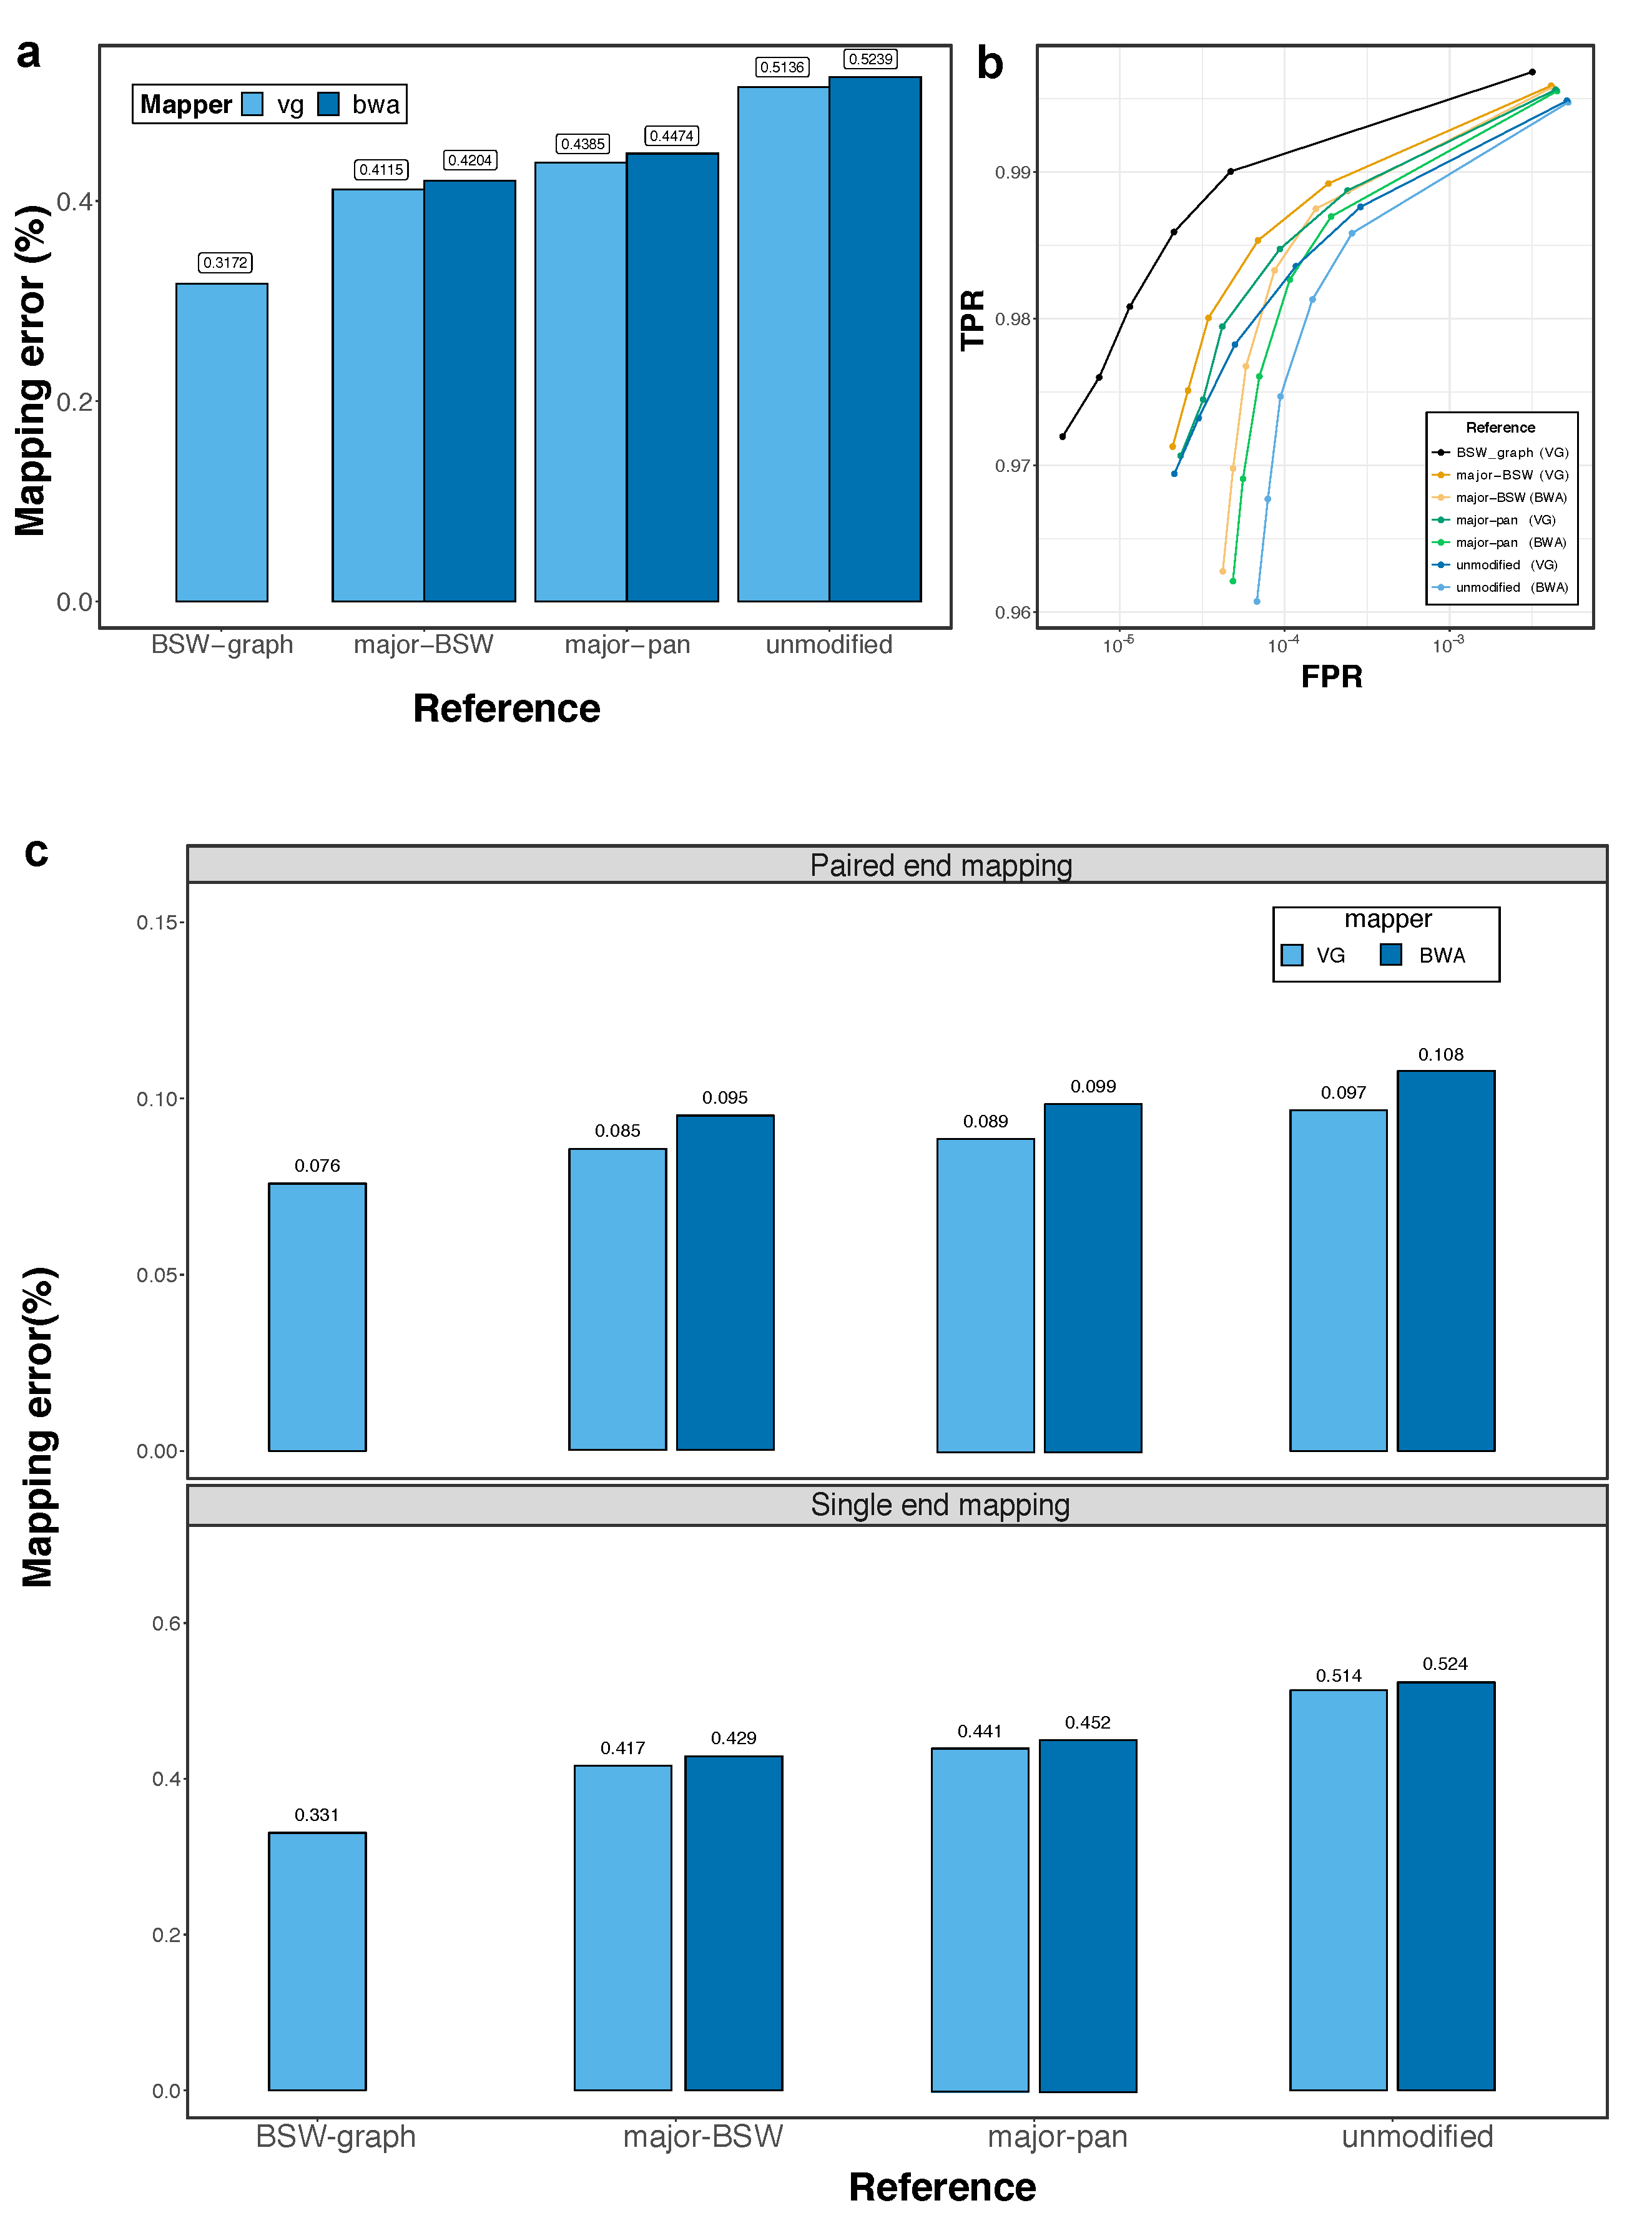
\includegraphics[width=0.7\textwidth]{paper2/supplement/sp313.pdf}
    \caption[ Single-end read mapping to consensus genome]{\textbf{Single-end read mapping accuracy using breed-specific
    augmented genome graphs and consensus linear reference sequences.} \\
    \small{(a) Dark and light blue represent the proportion of reads that mapped incorrectly
    using \emph{BWA mem} and \emph{vg}, respectively, to the BSW-specific augmented reference
    graph (BSW-graph), the BSW-specific (major-BSW) and multi-breed linear
    consensus sequence (major-pan) and the bovine linear reference sequence
    (unmodified). (b) True positive (sensitivity) and false positive mapping rate
    (specificity) parameterized based on the mapping quality. (c) Paired- and single-end
    read mapping accuracy using breed-specific augmented genome graphs and
    consensus linear reference sequences that were only adjusted at SNPs.}}
    \label{sup_fig:s313}
\end{figure}

\begin{figure}[!htb]
    \centering
    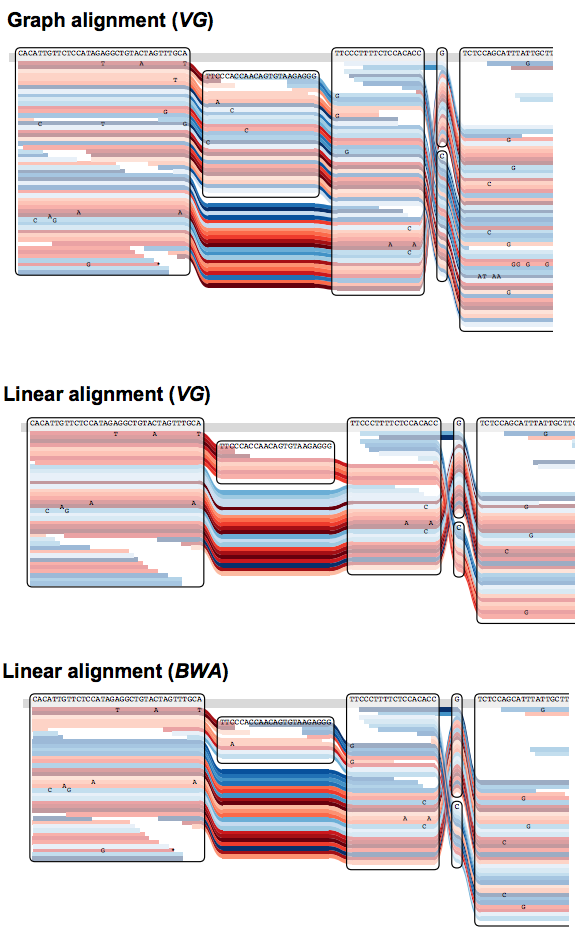
\includegraphics[width=0.8\textwidth]{paper2/supplement/sp314.png}
    \caption[ Graph alignment visualization.]{\textbf{Graph alignment visualization.} \\
    \small{Visualization of a 23-bp insertion at
    Chr10: 5,941,270 in graph and linear alignments using the \emph{sequence tube map} tool \citep{beyer2019sequence}. The variant was called heterozygous from the linear alignment,
    but the allelic ratio was highly biased towards the reference allele. Visual inspection
    suggests that more reads supporting the alternate allele are present in the graph
    alignments. Red and blue colour indicates forward and reverse reads, respectively.
    The reads from the linear alignment were realigned to the variation-aware graph for
    the purpose of the visualisation.}}
    \label{sup_fig:s314}
\end{figure}

\begin{figure}[!htb]
    \centering
    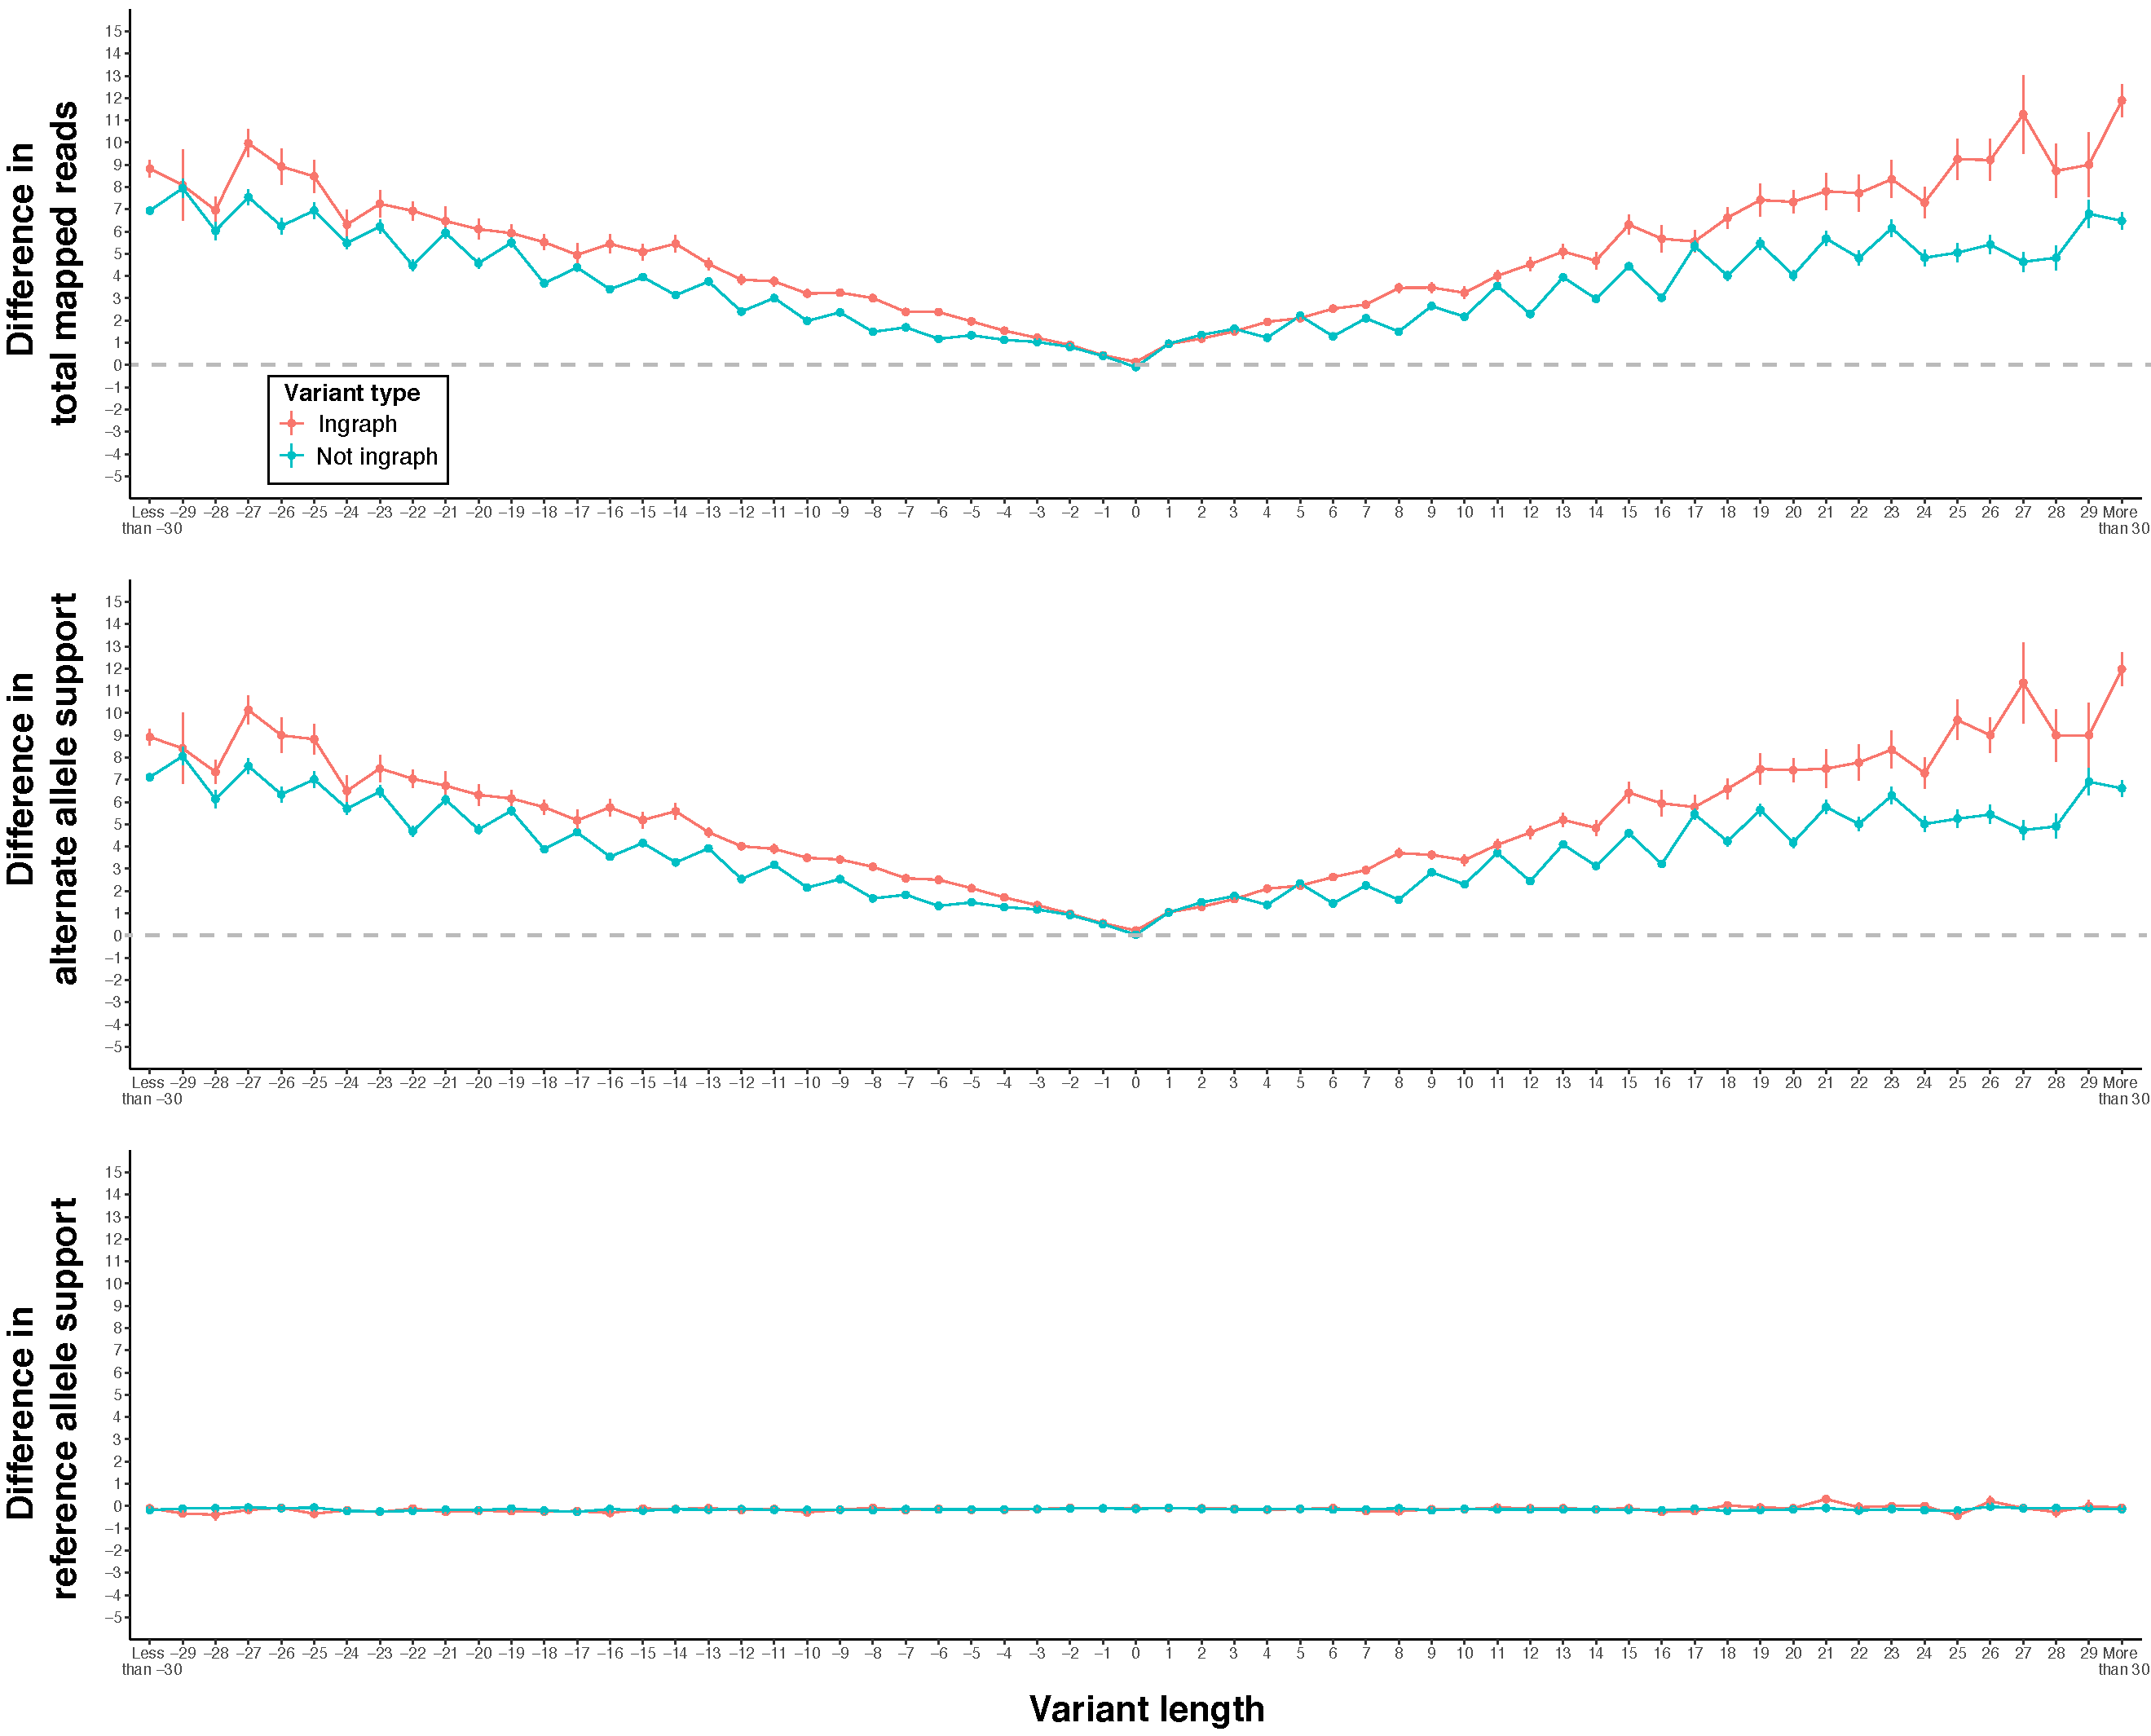
\includegraphics[width=\textwidth]{paper2/supplement/sp315.pdf}
    \caption[ Read support difference between reference and alternate alleles]{\textbf{Difference in the total of mapped reads, and reads support for
    reference and alternate alleles} \\
    \small{between the graph-based and BWA alignments for
    deletions, SNPs and insertions. Positive values indicate a larger number of reads for
    graph-based alignments. The dashed grey line indicates equal support for graphbased and linear alignments. The circles represent the mean ($\pm$ standard error of
    mean) values at a given variant length. Red and green colour indicates that the
    alternate allele is included and not included in the graph, respectively. }}
    \label{sup_fig:s315}
\end{figure}

\begin{figure}[!htb]
    \centering
    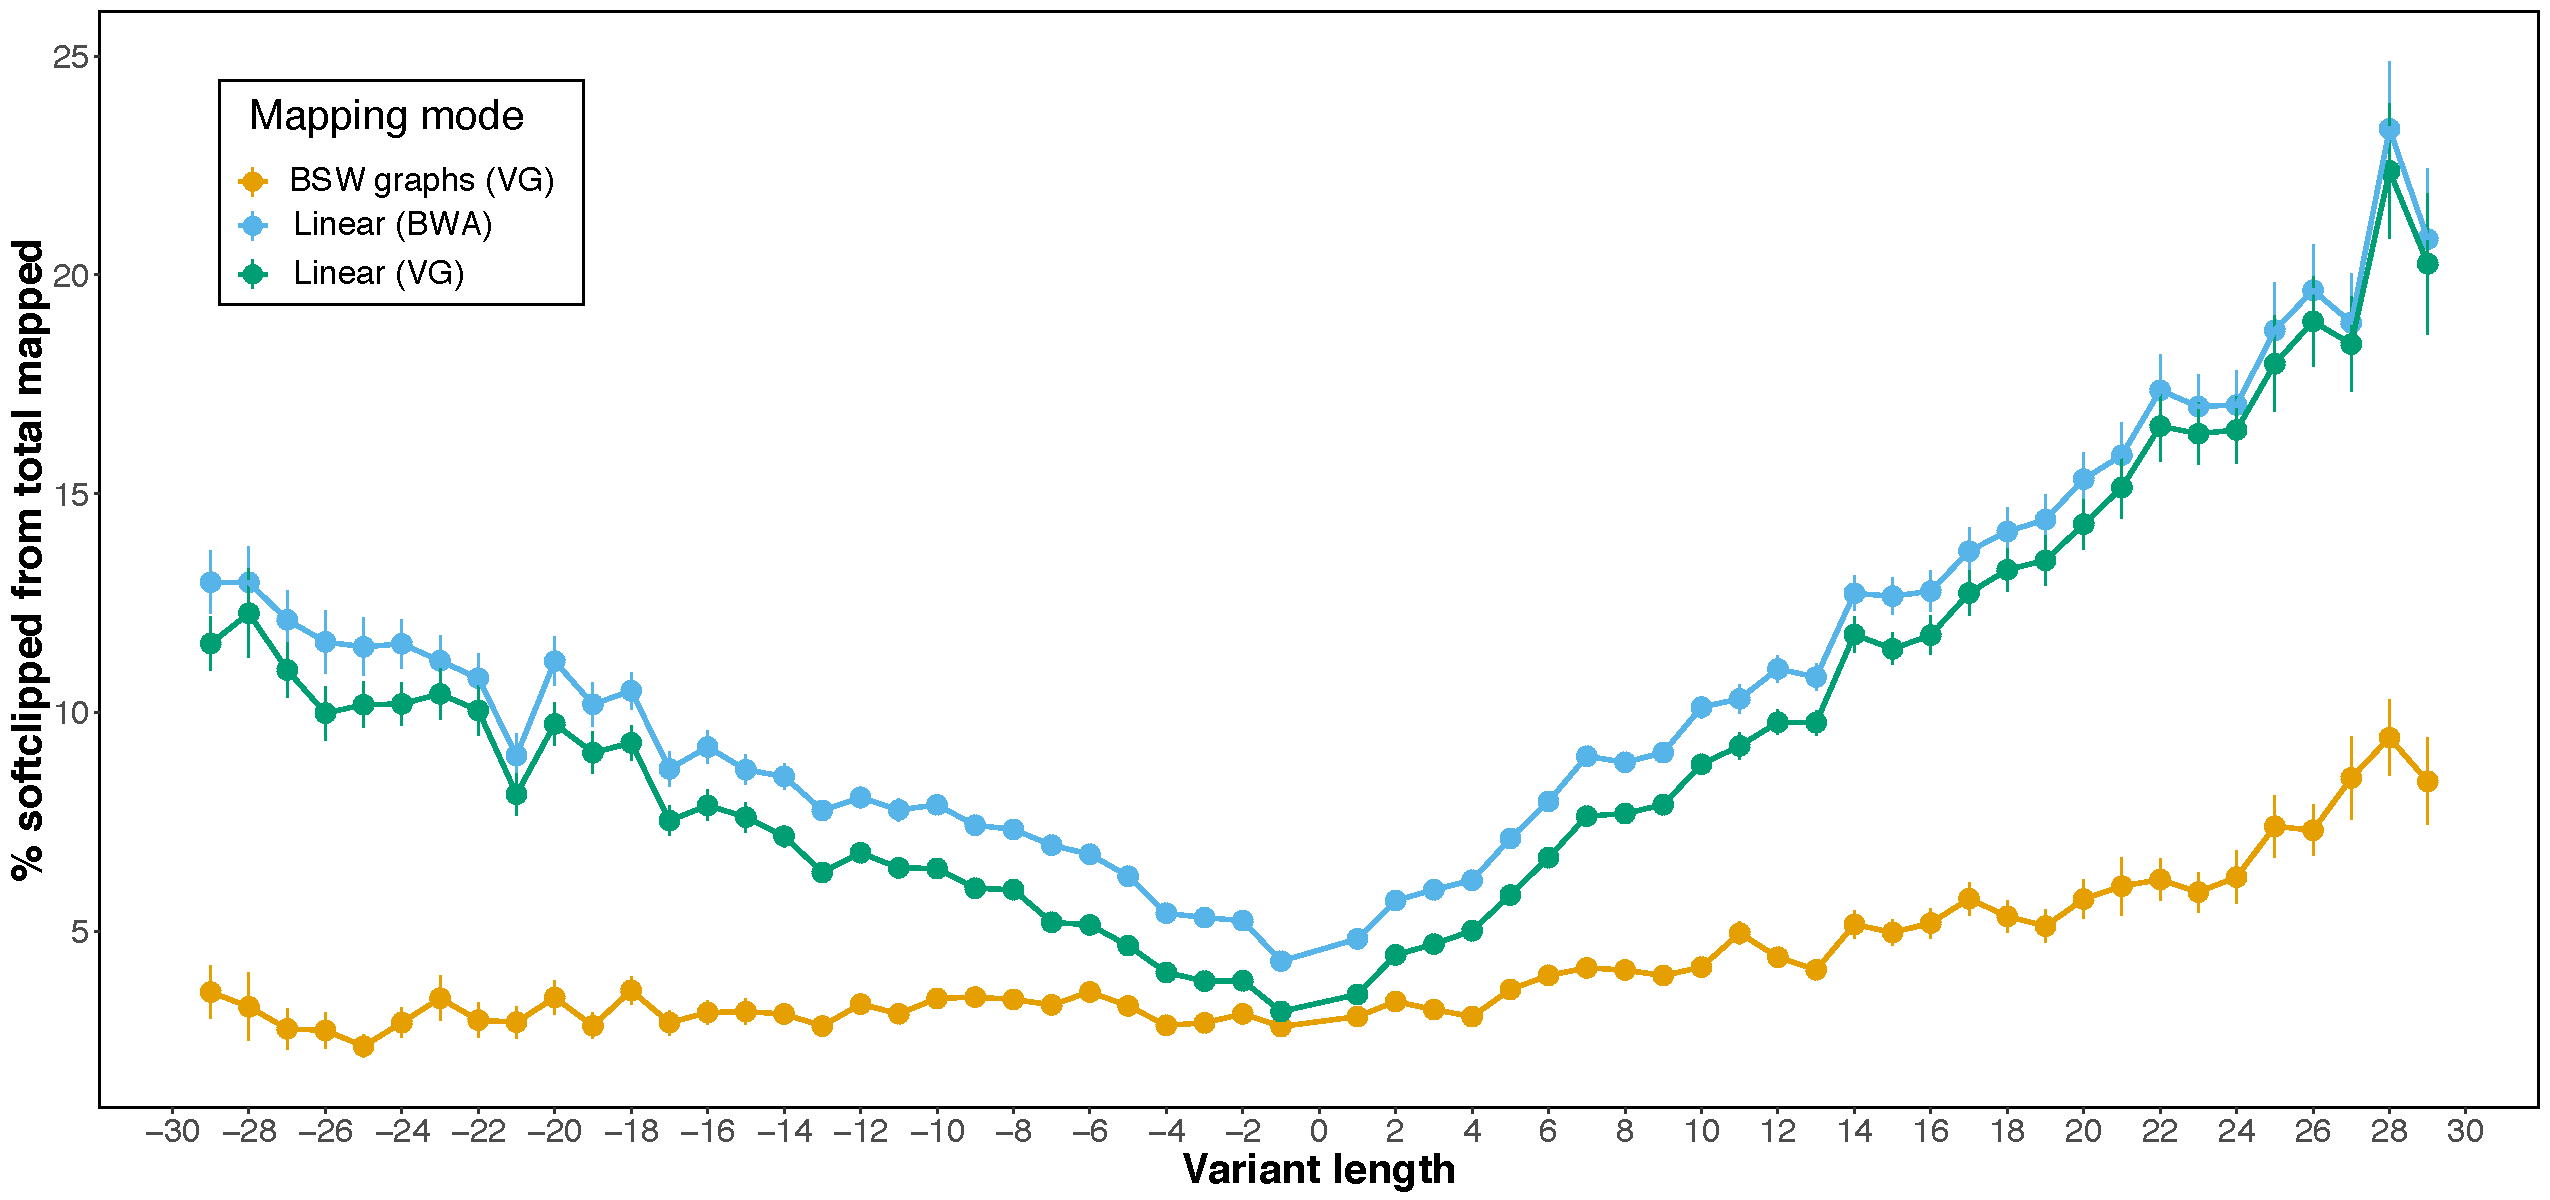
\includegraphics[width=\textwidth]{paper2/supplement/sp316.pdf}
    \caption[ Proportion of soft-clipped reads]{\textbf{Proportion of soft-clipped reads at heterozygous sites in graph
    (\emph{vg}) and linear (\emph{vg} and \emph{BWA}) alignments.} \\
    \small{We considered only variants for which
    the alternate allele was already included in the graph. The circles represent the
    mean ($\pm$ standard error of mean) values at a given variant length.}}
    \label{sup_fig:s316}
\end{figure}

\begin{figure}[!htb]
    \centering
    \includegraphics[width=0.8\textwidth]{paper2/supplement/sp317.pdf}
    \caption[ Genotype concordance matrices]{\textbf{Genotype concordance matrices for four quality parameters.} \\
    \small{For
    each metric, we divided the sum of the red cells by the sum of the cells within the
    green frame.}}
    \label{sup_fig:s317}
\end{figure}

\clearpage
% Supplementary notes

\subsection{}
\label{sup_not:s31}
\textbf{Comparison of variant prioritization approaches}

We applied FORGe \citep{pritt2018forge} to prioritize variants to be added to the Brown Swiss reference graph for chromosome 25. Specifically, we considered the four variant ranking approaches implemented in FORGe and compared the mapping accuracy from the
resulting graphs with a graph that was constructed with variants selected based on an allele frequency threshold.
\bigskip

The following prioritization approaches were investigated:
\begin{enumerate}
    \item  Pop Cov: variants ranked based on allele frequency
    \item  Pop Cov + blowup: variants ranked based on allele frequency and proximity (variants that are nearby receive lower scores)
    \item Hybrid: variants ranked based on allele frequency and how the variants affect the resulting k-mer profile of the genome graph (variants that would increase the
    repetiveness of the resulting graph receive lower scores)
    \item Hybrid + blowup: hybrid methods + considering variant proximity
    \item AF threshold: variants ranked based on allele frequency (AF, as applied in our paper).
\end{enumerate}

\bigskip

We refer to the FORGe paper \citep{pritt2018forge} for a detailed description on the
implementation of the variant prioritization methods 1-4.
For each prioritization approach, we constructed a number of graphs that included the top x\% of the ranked variants, where x ranged from 1 to 100 with steps of 10 (e.g., a graph constructed with x=10 included 34,715 out of 347,147 bta25 Brown Swiss variants). We then mapped paired-end reads simulated form a Brown Swiss animal (as detailed in the Material and Methods part of the main manuscript) to the graphs in order to calculate mapping accuracy.
\bigskip

Graphs constructed with variants that were prioritized solely using allele frequency (as applied in our current paper and the Pop Cov method of FORGe) enable the most accurate mapping of reads (\hyperlink{Table SN31}{Table SN31} and \hyperlink{Figure SN31}{Figure SN31}). Considering additional factors other than allele frequency did not lead to further accuracy improvements. The mapping accuracy of the Pop Cov and AF threshold strategies was virtually identical when the same number of variants was used. The most accurate Pop Cov approach corresponds to an alternate allele frequency threshold of 0.06. 
\bigskip
\newpage

\textbf{\hypertarget{Table SN31}{Table SN31}: Comparison of the most accurate graph from each ranking method}
\begin{center}
    \begin{tabular}{|l|l|l|} 
        \hline
        \textbf{Ranking methods}                            & \textbf{Minimum mapping error} & \multicolumn{1}{c|}{\begin{tabular}[c]{@{}c@{}}\textbf{Number of variants in the graphs }\\\textbf{with maximum accuracy}\end{tabular}}  \\ 
        \hline
        \rowcolor[rgb]{0.949,0.949,0.949} PopCov            & 0.0722                         & 208288                                                                                                                                   \\ 
        \hline
        PopCov + blowup                                     & 0.0730                         & 208288                                                                                                                                   \\ 
        \hline
        \rowcolor[rgb]{0.949,0.949,0.949} Variant frequency & 0.0723                         & 208288                                                                                                                                   \\ 
        \hline
        Hybrid                                              & 0.0749                         & 347147                                                                                                                                   \\ 
        \hline
        \rowcolor[rgb]{0.949,0.949,0.949} Hybrid + blowup   & 0.0749                         & 347147                                                                                                                                   \\
        \hline
        \end{tabular}
\end{center}

\bigskip

\begin{figure}[!htb]
    \centering
    \includegraphics[width=\textwidth]{paper2/supplement/forge_rank_pe.pdf}
    \caption*{\textbf{\hypertarget{Figure SN31}{Figure SN31}: Comparison of different variant prioritization strategies.} \\
    \small{Proportion of incorrectly mapped reads for graphs constructed with five variant prioritization approaches.}}
\end{figure}


\subsection{}
\label{sup_not:s32}
\textbf{Adjusted (tuned) linear mapping approach}
\bigskip

We followed the proposed approach outlined by \citep{grytten2020assessing} to adjust the default parameters of \emph{BWA mem} in order to also consider sub-optimal alignments.
First, we reduce the D value (default 0.5) to consider more alternative alignment positions.
However, the mapping performance changed only marginally.

\bigskip
Second, we ran \emph{Minimap2} in short read mode (-ax sr) to find all suboptimal alignments.
Subsequently, we retained for each read the read placement from either \emph{BWA mem} or
\emph{Minimap2} that had the higher alignment score. For reads that had identical alignment score
and position for both linear mappers, we retained the lower mapping quality score. For all
other cases, we retained the \emph{BWA mem} alignment.

\bigskip

We made two observations (\hyperlink{Figure SN32}{Figure SN32}):
\begin{enumerate}
    \item The overall mapping accuracy increased mainly due to a smaller number of incorrectly placed reads that had high mapping quality (MQ $>$ 10). This indicates that the tuned linear mapping approach assigns the quality of the alignments better.
    \item We found an improvement in mapping accuracy only on reads that are identical to the reference, but not on reads that contain variants.
\end{enumerate}

\bigskip

While Grytten et al. observed that an adjusted parameter setting of \emph{BWA mem} and subsequent application of \emph{Minimap2} led to considerable accuracy improvements, the gain in accuracy was low in our study. The proportion of simulated reads with variants was twice as high (19.16\% vs. 10.6\%) in our study than in Grytten et al., because the average number of polymorphic sites per genome was almost two-fold higher in cattle than humans.


\begin{figure}[!htb]
    \centering
    \includegraphics[width=\textwidth]{paper2/supplement/roc_tuned_comb.pdf}
    \caption*{\textbf{\hypertarget{Figure SN32}{Figure SN32}: Mapping accuracy of paired-end reads simulated form a Brown Swiss
    animal using different mapping approaches.} \\
    \small{(a) Proportion of simulated reads with mapping errors for different mapping scenarios. (b) True positive and false positive rate parameterized on mapping quality for the different scenarios.}}
\end{figure}

\clearpage

\subsection{}
\label{sup_not:s33}
\textbf{Integrating structural variants into the graphs}
\bigskip


We investigated the effect of including longer (structural) variants. For this purpose, we first called and genotyped structural variants using \emph{Delly} \citep{rausch2012delly} from 82 Brown Swiss samples that had been sequenced using short-reads (see Material and Methods part of the main manuscript). We discovered 157 precise SVs on bovine chromosome 25 that had an average length of 178 bp. We then combined these variants with 243,145 SNPs and Indels that were discovered using \emph{GATK}. We used the bta25 ARS-UCD1.2 reference as a backbone and constructed four graphs: (i) SNPs (+Indels) from \emph{GATK}, (i) SVs from \emph{Delly},
(iii) SNPs (+Indels) from \emph{GATK} + SVs from \emph{Delly}, (iv) empty (only the backbone, no variants). We simulated 10 million paired end reads from haplotypes of one Brown Swiss animal (SAMEA6272105, that had 121,996 SNPs + Indels and 57 SVs that were included in the graph). The simulated reads were mapped to the different graphs using \emph{vg}.

\bigskip

\textbf{\hypertarget{Table SN32}{Table SN32}: Mapping accuracy for graphs that contained different variant types} \\
MQ$=$0 and MQ $<$ 10 indicates the proportion of reads mapped with mapping quality 0 and
less than 10, respectively. 
\begin{center}
    \begin{tabular}{|l|l|l|l|l|} 
        \hline
        \textbf{Graphs}                            & \multicolumn{1}{c|}{\begin{tabular}[c]{@{}c@{}}\textbf{Variants }\\\textbf{in the graphs}\end{tabular}} & \textbf{MQ=0~(\%)} & \textbf{MQ\textless{}10 (\%)} & \textbf{Mapping error~(\%)}  \\ 
        \hline
        Linear                                     & 0                                                                                                       & 0.15474            & 0.22310                       & 0.08599                      \\ 
        \hline
        \rowcolor[rgb]{0.973,0.973,0.973} SNP      & 243,145                                                                                                 & 0.15366            & 0.21804                       & 0.07995                      \\ 
        \hline
        SV                                         & 157                                                                                                     & 0.15508            & 0.22390                       & 0.08629                      \\ 
        \hline
        \rowcolor[rgb]{0.973,0.973,0.973} SNP + SV & 243,145 + 157                                                                                           & 0.15458            & 0.21900                       & 0.08003                      \\
        \hline
        \end{tabular}
\end{center}

\bigskip 

Adding SVs that were detect from short sequencing reads to the graph marginally affected
the mapping performance. Actually, the mapping accuracy decreased slightly when SVs
were added. Read mapping accuracy improvements were attributable to the SNPs and
Indels detected using \emph{GATK}.

\clearpage

\begin{landscape}
\begin{table}
    \centering
    \caption[Comparison between human versus cattle autosomal variations]{\textbf{Properties of autosomal variants detected in human (JPT, GBR, STU, YRI) and bovine (HOL, FV, BSW, OBV) populations}}
    \label{sup_tab:s31}
    \begin{tabular}{|c|l|c|c|c|c|c|} 
    \hline
    Species                 & \multicolumn{1}{c|}{Population} & \begin{tabular}[c]{@{}c@{}}Number \\of samples\end{tabular} & Variant count & \begin{tabular}[c]{@{}c@{}}Average \\per sample\end{tabular} & \begin{tabular}[c]{@{}c@{}}Singleton\\~variants\end{tabular} & \begin{tabular}[c]{@{}c@{}}Variants with \\allele frequency \textless{} 0.05~\end{tabular}  \\ 
    \hline
    \multirow{4}{*}{Human}  & JPT                             & 104               & 12,433,397~~~ & 4,020,815          & 2,836,542 (22.81\%)  & 5,580,288 (44.88\%)                   \\ 
    \cline{2-7}
                            & GBR                             & 91                & 13,148,448    & 4,011,102          & 2,878,144 (21.88 \%) & 6,005,303 (45.67\%)                   \\ 
    \cline{2-7}
                            & STU                             & 102               & 15,264,479    & 4,096,457          & 4,024,478 (26.34\%)  & 7,915,678 (51.85\%)                   \\ 
    \cline{2-7}
                            & YRI                             & 108               & 22,420,039    & 4,863,955          & 4,702,120 (20.97\%)  & 12,431,887 (55.45\%)                  \\ 
    \hline
    \multirow{4}{*}{Cattle} & HOL                             & 49                & 16,762,842    & 6,841,965          & 1,713,642 (10.22\%)  & 3,964,699 (23.65\%)                   \\ 
    \cline{2-7}
                            & FV                              & 49                & 18,638,951~~  & 6,955,100          & 2,272,546 (12.19\%)  & 5,112,547 (27.42\%)                   \\ 
    \cline{2-7}
                            & BSW                             & 82                & 20,446,693    & 6,983,517          & 3,957,703 (19.35\%)  & 7,913,226 (38.70\%)                   \\ 
    \cline{2-7}
                            & OBV                             & 104               & 21,875,164    & 7,111,562          & 3,124,950 (14.28\%)  & 8,250,961 (37.71\%)                   \\
    \hline
    \end{tabular}
\end{table}

\newpage 

\begin{table}
    \centering
    \caption[Comparison variations in human chromosome 19 and chromosome 25 cattle]{\textbf{Properties of variants  detected on human chromosome 19 and bovine chromosome 25 in human (JPT, GBR, STU, YRI) and bovine (HOL, FV, BSW, OBV) populations}}
    \label{sup_tab:s32}
    \begin{tabular}{|c|l|c|c|c|c|c|} 
    \hline
    Species                 & \multicolumn{1}{c|}{Population} & \begin{tabular}[c]{@{}c@{}}Number \\of samples\end{tabular} & Variant count & \begin{tabular}[c]{@{}c@{}}Average \\per sample\end{tabular} & \begin{tabular}[c]{@{}c@{}}Singleton\\~variants\end{tabular} & \begin{tabular}[c]{@{}c@{}}Variants with \\allele frequency \textless{} 0.05~\end{tabular}  \\ 
    \hline
    \multirow{4}{*}{Human}  & JPT                             & 104                                                         & 291,303~~~    & 88,945                                                       & 66,944 (22.98\%)                                             & 135,289 (46.44\%)                                                                           \\ 
    \cline{2-7}
                            & GBR                             & 91                                                          & 306,304       & 90,988                                                       & 64,119 (20.93 \%)                                            & 138,076 (45.07\%)                                                                           \\ 
    \cline{2-7}
                            & STU                             & 102                                                         & 355,107~~~    & 94,253                                                       & 93,116 (26.22\%)                                             & 181,300 (51.05\%)                                                                           \\ 
    \cline{2-7}
                            & YRI                             & 108                                                         & 521,021       & 118,429                                                      & 106,734~~(20.49\%)                                           & 280,960 (53.92\%)                                                                           \\ 
    \hline
    \multirow{4}{*}{Cattle} & HOL                             & 49                                                          & 295,801       & 121,114                                                      & 30,543 (10.32\%)                                             & 67827 (22.92\%)                                                                             \\ 
    \cline{2-7}
                            & FV                              & 49                                                          & 336,390       & 125,597                                                      & 43,783 (13.01\%)                                             & 94,577 (28.11\%)                                                                            \\ 
    \cline{2-7}
                            & BSW                             & 82                                                          & 347,402       & 124,209                                                      & 53,773 (15.47\%)                                             & 128,990 (37.12\%)                                                                           \\ 
    \cline{2-7}
                            & OBV                             & 104                                                         & 387,855~~~    & 126,158                                                      & 47,498 (12.24\%)                                             & 144,958 (37.37\%)                                                                           \\
    \hline
    \end{tabular}
   \end{table}


\begin{table}
    \centering
    \caption[Concordance between array-called and sequence variant genotypes]{\textbf{Concordance between array-called and sequence variant genotypes that were discovered from either graph or linear alignments using \emph{Samtools}, \emph{GATK}, or \emph{Graphtyper}.}} 
    \small{Numbers represent average values ($\pm$ standard deviation) of 10 BSW animals for the raw (Full) and hard-filtered (Filtered) genotypes.}
    \bigskip
    \label{sup_tab:s33}
    \begin{tabular}{|l|l|l|l|l|l|l|} 
    \hline
    ~                       & \multicolumn{3}{c|}{Full}                                                              & \multicolumn{3}{c|}{Filtered}                                                           \\ 
    \hline
    \multicolumn{7}{|l|}{\textit{Samtools}}                                                                                                                                                                    \\ 
    \hline
    \multirow{2}{*}{~}      & \multicolumn{1}{c|}{Graph} & \multicolumn{1}{c|}{Linear} & \multicolumn{1}{c|}{Linear} & \multicolumn{1}{c|}{Graph} & \multicolumn{1}{c|}{Linear} & \multicolumn{1}{c|}{Linear}  \\ 
    \cline{2-7}
                            & \multicolumn{1}{c|}{VG}    & \multicolumn{1}{c|}{VG}     & \multicolumn{1}{c|}{BWA}    & \multicolumn{1}{c|}{VG}    & \multicolumn{1}{c|}{VG}     & \multicolumn{1}{c|}{BWA}     \\ 
    \hline
    Genotype concordance    & 98.50(1.07)                & 98.47(1.07)                 & 98.53(1.03)                 & 98.53(1.07)                & 98.50(1.07)                 & 98.55(1.04)                  \\ 
    \hline
    NR-sensitivity (Recall) & 98.53(0.37)                & 98.52(0.39)                 & 98.53(0.39)                 & 97.48(0.36)                & 97.45(0.35)                 & 97.53(0.36)                  \\ 
    \hline
    NR-discrepancy          & 2.21(1.60)                 & 2.24(1.60)                  & 2.17(1.55)                  & 2.17(1.60)                 & 2.20(1.61)                  & 2.13(1.56)                   \\ 
    \hline
    Precision               & 98.90(0.83)                & 98.89(0.83)                 & 98.93(0.81)                 & 98.91(0.83)                & 98.90(0.83)                 & 98.94(0.82)                  \\ 
    \hline
    \multicolumn{7}{|l|}{\textit{GATK}}                                                                                                                                                                        \\ 
    \hline
    Genotype concordance    & 97.26(2.24)                & 97.24(2.25)                 & 97.38(2.15)                 & 97.26(2.25)                & 97.25(2.25)                 & 97.39(2.15)                  \\ 
    \hline
    NR-sensitivity (Recall) & 98.17(0.94)                & 98.16(0.94)                 & 98.23(0.87)                 & 98.14(0.94)                & 98.12(0.94)                 & 98.18(0.87)                  \\ 
    \hline
    NR-discrepancy          & 4.09(3.38)                 & 4.10(3.39)                  & 3.89(3.23)                  & 4.08(3.38)                 & 4.09(3.39)                  & 3.88(3.23)                   \\ 
    \hline
    Precision               & 98.90(0.83)                & 98.90(0.83)                 & 98.94(0.80)                 & 98.91(0.83)                & 98.91(0.83)                 & 98.95(0.80)                  \\ 
    \hline
    \multicolumn{7}{|l|}{\textit{Graphtyper}}                                                                                                                                                                  \\ 
    \hline
    Genotype concordance    & 98.57(1.01)                & 98.57(1.01)                 & 98.61(0.97)                 & 98.61(1.03)                & 98.61(1.03)                 & 98.64(0.99)                  \\ 
    \hline
    NR-sensitivity (Recall) & 98.34(0.54)                & 98.36(0.55)                 & 98.37(0.53)                 & 96.14(0.54)                & 96.13(0.54)                 & 96.17(0.52)                  \\ 
    \hline
    NR-discrepancy          & 2.08(1.49)                 & 2.08(1.50)                  & 2.02(1.44)                  & 2.01(1.50)                 & 2.01(1.50)                  & 1.97(1.45)                   \\ 
    \hline
    Precision               & 98.85(0.80)                & 98.84(0.81)                 & 98.87(0.79)                 & 98.89(0.82)                & 98.89(0.82)                 & 98.91(0.80)                  \\
    \hline
    \end{tabular}
\end{table}
\end{landscape}

\clearpage

\begin{footnotesize}
\begin{longtable}{|c|c|c|c|c|c|c|} 
    \caption[Sample number accessions]{\textbf{Accession numbers of the animals} used for variant detection, read simulation, sequence read mapping and genotyping}
    \label{sup_tab:s34} \\
    \hline
    Accession     & Breed & \begin{tabular}[c]{@{}c@{}}Graph\\~construction\end{tabular} & Simulation & \begin{tabular}[c]{@{}c@{}}~~~Validation \\genotyping~\end{tabular} & \begin{tabular}[c]{@{}c@{}}Validation\\~Mapping bias\end{tabular} & Coverage  
    \endfirsthead 
    \multicolumn{1}{c}{\small{\emph{Continuation of Table \ref{sup_tab:s34}}}}\\
    \hline
    Accession     & Breed & \begin{tabular}[c]{@{}c@{}}Graph\\~construction\end{tabular} & Simulation & \begin{tabular}[c]{@{}c@{}}~~~Validation \\genotyping~\end{tabular} & \begin{tabular}[c]{@{}c@{}}Validation\\~Mapping bias\end{tabular} & Coverage  
    \endhead
    \hline
    SAMEA4827645  & OBV   & x                                                            & ~          & ~                                                                           & ~                                                                 & 14.41     \\ 
    \hline
    SAMEA4827646  & OBV   & x                                                            & ~          & ~                                                                           & ~                                                                 & 12.9      \\ 
    \hline
    SAMEA4827647  & OBV   & x                                                            & ~          & ~                                                                           & ~                                                                 & 14.79     \\ 
    \hline
    SAMEA4827648  & OBV   & x                                                            & ~          & ~                                                                           & ~                                                                 & 10.76     \\ 
    \hline
    SAMEA4827649  & OBV   & x                                                            & ~          & ~                                                                           & ~                                                                 & 11.55     \\ 
    \hline
    SAMEA4827650  & OBV   & x                                                            & ~          & ~                                                                           & ~                                                                 & 10.29     \\ 
    \hline
    SAMEA4827651  & OBV   & x                                                            & ~          & ~                                                                           & ~                                                                 & 14.76     \\ 
    \hline
    SAMEA4827652  & OBV   & x                                                            & ~          & ~                                                                           & ~                                                                 & 10.65     \\ 
    \hline
    SAMEA4827653  & OBV   & x                                                            & ~          & ~                                                                           & ~                                                                 & 9.69      \\ 
    \hline
    SAMEA4827654  & OBV   & x                                                            & ~          & ~                                                                           & ~                                                                 & 10.72     \\ 
    \hline
    SAMEA4827655  & OBV   & x                                                            & ~          & ~                                                                           & ~                                                                 & 11.32     \\ 
    \hline
    SAMEA4827656  & OBV   & x                                                            & ~          & ~                                                                           & ~                                                                 & 11.83     \\ 
    \hline
    SAMEA4827657  & OBV   & x                                                            & ~          & ~                                                                           & ~                                                                 & 8.47      \\ 
    \hline
    SAMEA4827658  & OBV   & x                                                            & ~          & ~                                                                           & ~                                                                 & 9.69      \\ 
    \hline
    SAMEA4827659  & OBV   & x                                                            & ~          & ~                                                                           & ~                                                                 & 9.52      \\ 
    \hline
    SAMEA4827660  & OBV   & x                                                            & ~          & ~                                                                           & ~                                                                 & 10.04     \\ 
    \hline
    SAMEA4827661  & OBV   & x                                                            & ~          & ~                                                                           & ~                                                                 & 9.68      \\ 
    \hline
    SAMEA4827662  & OBV   & x                                                            & ~          & ~                                                                           & ~                                                                 & 17.37     \\ 
    \hline
    SAMEA4827663  & OBV   & x                                                            & ~          & ~                                                                           & ~                                                                 & 11.2      \\ 
    \hline
    SAMEA4827664  & OBV   & x                                                            & ~          & ~                                                                           & ~                                                                 & 11.29     \\ 
    \hline
    SAMEA4827665  & OBV   & x                                                            & ~          & ~                                                                           & ~                                                                 & 13.07     \\ 
    \hline
    SAMEA4827666  & OBV   & x                                                            & ~          & ~                                                                           & ~                                                                 & 11.23     \\ 
    \hline
    SAMEA4827667  & OBV   & x                                                            & ~          & ~                                                                           & ~                                                                 & 10.99     \\ 
    \hline
    SAMEA4827668  & OBV   & x                                                            & ~          & ~                                                                           & ~                                                                 & 10.93     \\ 
    \hline
    SAMEA4827669  & OBV   & x                                                            & ~          & ~                                                                           & ~                                                                 & 12.89     \\ 
    \hline
    SAMEA4827670  & OBV   & x                                                            & ~          & ~                                                                           & ~                                                                 & 12.18     \\ 
    \hline
    SAMEA4827671  & OBV   & x                                                            & ~          & ~                                                                           & ~                                                                 & 11.35     \\ 
    \hline
    SAMEA4827672  & OBV   & x                                                            & ~          & ~                                                                           & ~                                                                 & 10.49     \\ 
    \hline
    SAMEA4827673  & OBV   & x                                                            & ~          & ~                                                                           & ~                                                                 & 10.31     \\ 
    \hline
    SAMEA4827674  & OBV   & x                                                            & ~          & ~                                                                           & ~                                                                 & 12.58     \\ 
    \hline
    SAMEA5059741  & OBV   & x                                                            & ~          & ~                                                                           & ~                                                                 & 4.58      \\ 
    \hline
    SAMEA5059742  & OBV   & x                                                            & ~          & ~                                                                           & ~                                                                 & 3.76      \\ 
    \hline
    SAMEA5059743  & OBV   & x                                                            & x          & ~                                                                           & ~                                                                 & 22.33     \\ 
    \hline
    SAMEA5059744  & OBV   & x                                                            & ~          & ~                                                                           & ~                                                                 & 3.93      \\ 
    \hline
    SAMEA5059745  & OBV   & x                                                            & ~          & ~                                                                           & ~                                                                 & 4.31      \\ 
    \hline
    SAMEA5059746  & OBV   & x                                                            & ~          & ~                                                                           & ~                                                                 & 4.29      \\ 
    \hline
    SAMEA5059747  & OBV   & x                                                            & ~          & ~                                                                           & ~                                                                 & 4.58      \\ 
    \hline
    SAMEA5059748  & OBV   & x                                                            & ~          & ~                                                                           & ~                                                                 & 5.08      \\ 
    \hline
    SAMEA5059749  & OBV   & x                                                            & ~          & ~                                                                           & ~                                                                 & 5.19      \\ 
    \hline
    SAMEA5059750  & OBV   & x                                                            & ~          & ~                                                                           & ~                                                                 & 3.91      \\ 
    \hline
    SAMEA5059751  & OBV   & x                                                            & ~          & ~                                                                           & ~                                                                 & 5.59      \\ 
    \hline
    SAMEA5059752  & OBV   & x                                                            & ~          & ~                                                                           & ~                                                                 & 3.89      \\ 
    \hline
    SAMEA5059753  & OBV   & x                                                            & ~          & ~                                                                           & ~                                                                 & 4.18      \\ 
    \hline
    SAMEA5059754  & OBV   & x                                                            & ~          & ~                                                                           & ~                                                                 & 3.49      \\ 
    \hline
    SAMEA5059755  & OBV   & x                                                            & ~          & ~                                                                           & ~                                                                 & 7.49      \\ 
    \hline
    SAMEA5059756  & OBV   & x                                                            & ~          & ~                                                                           & ~                                                                 & 6.65      \\ 
    \hline
    SAMEA5059757  & OBV   & x                                                            & ~          & ~                                                                           & ~                                                                 & 5.74      \\ 
    \hline
    SAMEA5059758  & OBV   & x                                                            & ~          & ~                                                                           & ~                                                                 & 5.1       \\ 
    \hline
    SAMEA6272117  & OBV   & x                                                            & ~          & ~                                                                           & ~                                                                 & 6.43      \\ 
    \hline
    SAMEA5059759  & OBV   & x                                                            & ~          & ~                                                                           & ~                                                                 & 3.97      \\ 
    \hline
    SAMEA5159792  & BSW   & x                                                            & ~          & ~                                                                           & ~                                                                 & 10.68     \\ 
    \hline
    SAMEA5159791  & BSW   & x                                                            & ~          & ~                                                                           & ~                                                                 & 10.22     \\ 
    \hline
    SAMEA5159788  & BSW   & x                                                            & ~          & ~                                                                           & ~                                                                 & 10.71     \\ 
    \hline
    SAMEA5159783  & BSW   & x                                                            & ~          & ~                                                                           & ~                                                                 & 11.91     \\ 
    \hline
    SAMEA5159785  & BSW   & x                                                            & ~          & ~                                                                           & ~                                                                 & 11.94     \\ 
    \hline
    SAMEA5159799  & BSW   & x                                                            & ~          & ~                                                                           & ~                                                                 & 10.25     \\ 
    \hline
    SAMEA5159787  & BSW   & x                                                            & ~          & ~                                                                           & ~                                                                 & 13.63     \\ 
    \hline
    SAMEA5159761  & BSW   & x                                                            & ~          & ~                                                                           & ~                                                                 & 16.46     \\ 
    \hline
    SAMEA5159782  & BSW   & x                                                            & ~          & ~                                                                           & ~                                                                 & 11.47     \\ 
    \hline
    SAMEA5159775  & BSW   & x                                                            & ~          & ~                                                                           & ~                                                                 & 10.14     \\ 
    \hline
    SAMEA5159786  & BSW   & x                                                            & ~          & ~                                                                           & ~                                                                 & 12.04     \\ 
    \hline
    SAMEA5159784  & BSW   & x                                                            & ~          & ~                                                                           & ~                                                                 & 11.88     \\ 
    \hline
    SAMEA5159798  & BSW   & x                                                            & ~          & ~                                                                           & ~                                                                 & 12.79     \\ 
    \hline
    SAMEA5159781  & BSW   & x                                                            & ~          & ~                                                                           & ~                                                                 & 12.65     \\ 
    \hline
    SAMEA5159780  & BSW   & x                                                            & ~          & ~                                                                           & ~                                                                 & 12.41     \\ 
    \hline
    SAMEA5159777  & BSW   & x                                                            & ~          & ~                                                                           & ~                                                                 & 9.8       \\ 
    \hline
    SAMEA5159797  & BSW   & x                                                            & ~          & ~                                                                           & ~                                                                 & 11.98     \\ 
    \hline
    SAMEA5159774  & BSW   & x                                                            & ~          & ~                                                                           & ~                                                                 & 9.46      \\ 
    \hline
    SAMEA5159769  & BSW   & x                                                            & ~          & ~                                                                           & ~                                                                 & 12.3      \\ 
    \hline
    SAMEA5159778  & BSW   & x                                                            & ~          & ~                                                                           & ~                                                                 & 13.03     \\ 
    \hline
    SAMEA5159771  & BSW   & x                                                            & ~          & ~                                                                           & ~                                                                 & 10.92     \\ 
    \hline
    SAMEA5159779  & BSW   & x                                                            & ~          & ~                                                                           & ~                                                                 & 10.63     \\ 
    \hline
    SAMEA5159772  & BSW   & x                                                            & ~          & ~                                                                           & ~                                                                 & 11.88     \\ 
    \hline
    SAMEA5159773  & BSW   & x                                                            & ~          & ~                                                                           & ~                                                                 & 10.77     \\ 
    \hline
    SAMEA5159793  & BSW   & x                                                            & ~          & ~                                                                           & ~                                                                 & 12.6      \\ 
    \hline
    SAMEA5159770  & BSW   & x                                                            & ~          & ~                                                                           & ~                                                                 & 10.01     \\ 
    \hline
    SAMEA5159795  & OBV   & x                                                            & ~          & ~                                                                           & ~                                                                 & 12.58     \\ 
    \hline
    SAMEA5159768  & OBV   & x                                                            & ~          & ~                                                                           & ~                                                                 & 8.69      \\ 
    \hline
    SAMEA5159796  & OBV   & x                                                            & ~          & ~                                                                           & ~                                                                 & 11.39     \\ 
    \hline
    SAMEA5159789  & OBV   & x                                                            & ~          & ~                                                                           & ~                                                                 & 10.27     \\ 
    \hline
    SAMEA5159790  & OBV   & x                                                            & ~          & ~                                                                           & ~                                                                 & 10.52     \\ 
    \hline
    SAMEA5159794  & OBV   & x                                                            & ~          & ~                                                                           & ~                                                                 & 11.46     \\ 
    \hline
    SAMEA5159776  & OBV   & x                                                            & ~          & ~                                                                           & ~                                                                 & 9.71      \\ 
    \hline
    SAMEA5159767  & OBV   & x                                                            & ~          & ~                                                                           & ~                                                                 & 10.17     \\ 
    \hline
    SAMN05216093  & OBV   & x                                                            & ~          & ~                                                                           & ~                                                                 & 10.85     \\ 
    \hline
    SAMN05216095  & OBV   & x                                                            & ~          & ~                                                                           & ~                                                                 & 11.12     \\ 
    \hline
    SAMN05216094  & OBV   & x                                                            & ~          & ~                                                                           & ~                                                                 & 10.64     \\ 
    \hline
    SAMN05216096  & OBV   & x                                                            & ~          & ~                                                                           & ~                                                                 & 11.51     \\ 
    \hline
    SAMEA6272131  & FV    & x                                                            & ~          & ~                                                                           & ~                                                                 & 13.4      \\ 
    \hline
    SAMEA6272130  & FV    & x                                                            & ~          & ~                                                                           & ~                                                                 & 10.41     \\ 
    \hline
    SAMEA4644727  & BSW   & x                                                            & ~          & ~                                                                           & ~                                                                 & 14.86     \\ 
    \hline
    SAMEA4644728  & BSW   & x                                                            & ~          & ~                                                                           & ~                                                                 & 14.86     \\ 
    \hline
    SAMEA19864918 & BSW   & x                                                            & ~          & ~                                                                           & ~                                                                 & 9.23      \\ 
    \hline
    SAMEA4644765  & BSW   & x                                                            & ~          & ~                                                                           & ~                                                                 & 12.14     \\ 
    \hline
    SAMEA4644766  & BSW   & x                                                            & ~          & ~                                                                           & ~                                                                 & 16.48     \\ 
    \hline
    SAMEA4644768  & OBV   & x                                                            & ~          & ~                                                                           & ~                                                                 & 13.41     \\ 
    \hline
    SAMEA4644769  & BSW   & x                                                            & ~          & ~                                                                           & ~                                                                 & 16.04     \\ 
    \hline
    SAMEA19312918 & BSW   & x                                                            & ~          & ~                                                                           & ~                                                                 & 4.43      \\ 
    \hline
    SAMEA19313668 & BSW   & x                                                            & ~          & ~                                                                           & ~                                                                 & 7.13      \\ 
    \hline
    SAMEA19314418 & BSW   & x                                                            & ~          & ~                                                                           & ~                                                                 & 10.99     \\ 
    \hline
    SAMEA19315168 & BSW   & x                                                            & ~          & ~                                                                           & ~                                                                 & 9.7       \\ 
    \hline
    SAMEA19318918 & BSW   & x                                                            & ~          & ~                                                                           & ~                                                                 & 6.9       \\ 
    \hline
    SAMEA19323418 & BSW   & x                                                            & ~          & ~                                                                           & ~                                                                 & 18.83     \\ 
    \hline
    SAMEA4644754  & BSW   & x                                                            & ~          & ~                                                                           & ~                                                                 & 15.25     \\ 
    \hline
    SAMEA4644755  & BSW   & x                                                            & ~          & ~                                                                           & ~                                                                 & 13.58     \\ 
    \hline
    SAMEA4644756  & BSW   & x                                                            & ~          & ~                                                                           & ~                                                                 & 13.88     \\ 
    \hline
    SAMEA4644730  & OBV   & x                                                            & ~          & ~                                                                           & ~                                                                 & 14.85     \\ 
    \hline
    SAMEA4644734  & OBV   & x                                                            & ~          & ~                                                                           & ~                                                                 & 15.3      \\ 
    \hline
    SAMEA4644735  & BSW   & x                                                            & ~          & ~                                                                           & ~                                                                 & 9.43      \\ 
    \hline
    SAMEA4644757  & BSW   & x                                                            & ~          & ~                                                                           & ~                                                                 & 11.36     \\ 
    \hline
    SAMEA4644739  & BSW   & x                                                            & ~          & ~                                                                           & ~                                                                 & 14.13     \\ 
    \hline
    SAMEA4644740  & OBV   & x                                                            & ~          & ~                                                                           & ~                                                                 & 15.73     \\ 
    \hline
    SAMEA4644741  & BSW   & x                                                            & ~          & ~                                                                           & ~                                                                 & 15.57     \\ 
    \hline
    SAMEA4644742  & BSW   & x                                                            & ~          & ~                                                                           & ~                                                                 & 15.68     \\ 
    \hline
    SAMEA4644758  & BSW   & x                                                            & ~          & ~                                                                           & ~                                                                 & 13        \\ 
    \hline
    SAMEA4644743  & BSW   & x                                                            & ~          & ~                                                                           & ~                                                                 & 15.46     \\ 
    \hline
    SAMEA4644749  & OBV   & x                                                            & ~          & ~                                                                           & ~                                                                 & 13.85     \\ 
    \hline
    SAMEA4644750  & OBV   & x                                                            & ~          & ~                                                                           & ~                                                                 & 15.25     \\ 
    \hline
    SAMEA4644762  & BSW   & x                                                            & ~          & ~                                                                           & ~                                                                 & 13.92     \\ 
    \hline
    SAMEA4644763  & BSW   & x                                                            & ~          & ~                                                                           & ~                                                                 & 11.62     \\ 
    \hline
    SAMEA4644764  & OBV   & x                                                            & ~          & ~                                                                           & ~                                                                 & 10.57     \\ 
    \hline
    SAMN07692225  & BSW   & x                                                            & ~          & ~                                                                           & ~                                                                 & 10.72     \\ 
    \hline
    SAMN02671625  & FV    & x                                                            & ~          & ~                                                                           & ~                                                                 & 5.06      \\ 
    \hline
    SAMN02671626  & FV    & x                                                            & x          & ~                                                                           & ~                                                                 & 23.24     \\ 
    \hline
    SAMN02671627  & FV    & x                                                            & ~          & ~                                                                           & ~                                                                 & 6.32      \\ 
    \hline
    SAMN02671628  & FV    & x                                                            & ~          & ~                                                                           & ~                                                                 & 4.95      \\ 
    \hline
    SAMN02671629  & FV    & x                                                            & ~          & ~                                                                           & ~                                                                 & 8.41      \\ 
    \hline
    SAMN02671630  & FV    & x                                                            & ~          & ~                                                                           & ~                                                                 & 4.88      \\ 
    \hline
    SAMN02671631  & FV    & x                                                            & ~          & ~                                                                           & ~                                                                 & 4.77      \\ 
    \hline
    SAMN02671632  & FV    & x                                                            & ~          & ~                                                                           & ~                                                                 & 7.64      \\ 
    \hline
    SAMN02671633  & FV    & x                                                            & ~          & ~                                                                           & ~                                                                 & 3.59      \\ 
    \hline
    SAMN02671634  & FV    & x                                                            & ~          & ~                                                                           & ~                                                                 & 7.67      \\ 
    \hline
    SAMN02671635  & FV    & x                                                            & ~          & ~                                                                           & ~                                                                 & 6.37      \\ 
    \hline
    SAMN02671636  & FV    & x                                                            & ~          & ~                                                                           & ~                                                                 & 6.26      \\ 
    \hline
    SAMN02671637  & FV    & x                                                            & ~          & ~                                                                           & ~                                                                 & 3.79      \\ 
    \hline
    SAMN02671638  & FV    & x                                                            & ~          & ~                                                                           & ~                                                                 & 3.95      \\ 
    \hline
    SAMN02671639  & FV    & x                                                            & ~          & ~                                                                           & ~                                                                 & 7.21      \\ 
    \hline
    SAMN02671640  & FV    & x                                                            & ~          & ~                                                                           & ~                                                                 & 8.62      \\ 
    \hline
    SAMN02671641  & FV    & x                                                            & ~          & ~                                                                           & ~                                                                 & 6.08      \\ 
    \hline
    SAMN02671642  & FV    & x                                                            & ~          & ~                                                                           & ~                                                                 & 5.47      \\ 
    \hline
    SAMN02671643  & FV    & x                                                            & ~          & ~                                                                           & ~                                                                 & 5.03      \\ 
    \hline
    SAMN02671644  & FV    & x                                                            & ~          & ~                                                                           & ~                                                                 & 4.35      \\ 
    \hline
    SAMN02671645  & FV    & x                                                            & ~          & ~                                                                           & ~                                                                 & 5.06      \\ 
    \hline
    SAMN02671646  & FV    & x                                                            & ~          & ~                                                                           & ~                                                                 & 5.79      \\ 
    \hline
    SAMN02671647  & FV    & x                                                            & ~          & ~                                                                           & ~                                                                 & 5.2       \\ 
    \hline
    SAMN02671648  & FV    & x                                                            & ~          & ~                                                                           & ~                                                                 & 5.81      \\ 
    \hline
    SAMN02671649  & FV    & x                                                            & ~          & ~                                                                           & ~                                                                 & 5.32      \\ 
    \hline
    SAMN02671650  & FV    & x                                                            & ~          & ~                                                                           & ~                                                                 & 5.34      \\ 
    \hline
    SAMN02671651  & FV    & x                                                            & ~          & ~                                                                           & ~                                                                 & 4.51      \\ 
    \hline
    SAMN02671652  & FV    & x                                                            & ~          & ~                                                                           & ~                                                                 & 7.48      \\ 
    \hline
    SAMN02671653  & FV    & x                                                            & ~          & ~                                                                           & ~                                                                 & 7.5       \\ 
    \hline
    SAMN02671654  & FV    & x                                                            & ~          & ~                                                                           & ~                                                                 & 7.6       \\ 
    \hline
    SAMN02671655  & FV    & x                                                            & ~          & ~                                                                           & ~                                                                 & 7.19      \\ 
    \hline
    SAMN02671656  & FV    & x                                                            & ~          & ~                                                                           & ~                                                                 & 5.4       \\ 
    \hline
    SAMN02671657  & FV    & x                                                            & ~          & ~                                                                           & ~                                                                 & 5.61      \\ 
    \hline
    SAMN02671658  & FV    & x                                                            & ~          & ~                                                                           & ~                                                                 & 4.91      \\ 
    \hline
    SAMN02671659  & FV    & x                                                            & ~          & ~                                                                           & ~                                                                 & 4.83      \\ 
    \hline
    SAMN02671661  & FV    & x                                                            & ~          & ~                                                                           & ~                                                                 & 5.58      \\ 
    \hline
    SAMN02671662  & FV    & x                                                            & ~          & ~                                                                           & ~                                                                 & 6.08      \\ 
    \hline
    SAMN02671663  & FV    & x                                                            & ~          & ~                                                                           & ~                                                                 & 5.06      \\ 
    \hline
    SAMN02671664  & FV    & x                                                            & ~          & ~                                                                           & ~                                                                 & 7.95      \\ 
    \hline
    SAMN02671665  & FV    & x                                                            & ~          & ~                                                                           & ~                                                                 & 6.53      \\ 
    \hline
    SAMN02671666  & FV    & x                                                            & ~          & ~                                                                           & ~                                                                 & 6.06      \\ 
    \hline
    SAMN02671667  & FV    & x                                                            & ~          & ~                                                                           & ~                                                                 & 8.13      \\ 
    \hline
    SAMN02671572  & HOL   & x                                                            & ~          & ~                                                                           & ~                                                                 & 6.79      \\ 
    \hline
    SAMN02671574  & HOL   & x                                                            & ~          & ~                                                                           & ~                                                                 & 10.25     \\ 
    \hline
    SAMN02671576  & HOL   & x                                                            & ~          & ~                                                                           & ~                                                                 & 5.02      \\ 
    \hline
    SAMN02671578  & HOL   & x                                                            & ~          & ~                                                                           & ~                                                                 & 19.78     \\ 
    \hline
    SAMN02671580  & HOL   & x                                                            & ~          & ~                                                                           & ~                                                                 & 10.52     \\ 
    \hline
    SAMN02671582  & HOL   & x                                                            & ~          & ~                                                                           & ~                                                                 & 15.22     \\ 
    \hline
    SAMN02671584  & HOL   & x                                                            & x          & ~                                                                           & ~                                                                 & 29.97     \\ 
    \hline
    SAMN02671586  & HOL   & x                                                            & ~          & ~                                                                           & ~                                                                 & 17.21     \\ 
    \hline
    SAMN02671588  & HOL   & x                                                            & ~          & ~                                                                           & ~                                                                 & 16.99     \\ 
    \hline
    SAMN02671590  & HOL   & x                                                            & ~          & ~                                                                           & ~                                                                 & 13.79     \\ 
    \hline
    SAMN02671592  & HOL   & x                                                            & ~          & ~                                                                           & ~                                                                 & 16.31     \\ 
    \hline
    SAMN02671594  & HOL   & x                                                            & ~          & ~                                                                           & ~                                                                 & 19.56     \\ 
    \hline
    SAMN02671596  & HOL   & x                                                            & ~          & ~                                                                           & ~                                                                 & 16.43     \\ 
    \hline
    SAMN02671455  & HOL   & x                                                            & ~          & ~                                                                           & ~                                                                 & 9.23      \\ 
    \hline
    SAMN02671457  & HOL   & x                                                            & ~          & ~                                                                           & ~                                                                 & 10.28     \\ 
    \hline
    SAMN02671459  & HOL   & x                                                            & ~          & ~                                                                           & ~                                                                 & 8.4       \\ 
    \hline
    SAMN02671461  & HOL   & x                                                            & ~          & ~                                                                           & ~                                                                 & 9.47      \\ 
    \hline
    SAMN02671463  & HOL   & x                                                            & ~          & ~                                                                           & ~                                                                 & 6.36      \\ 
    \hline
    SAMN02671465  & HOL   & x                                                            & ~          & ~                                                                           & ~                                                                 & 10.61     \\ 
    \hline
    SAMN02671467  & HOL   & x                                                            & ~          & ~                                                                           & ~                                                                 & 9.78      \\ 
    \hline
    SAMN02671469  & HOL   & x                                                            & ~          & ~                                                                           & ~                                                                 & 9.13      \\ 
    \hline
    SAMN02671471  & HOL   & x                                                            & ~          & ~                                                                           & ~                                                                 & 6.49      \\ 
    \hline
    SAMN02671473  & HOL   & x                                                            & ~          & ~                                                                           & ~                                                                 & 8.71      \\ 
    \hline
    SAMN02671475  & HOL   & x                                                            & ~          & ~                                                                           & ~                                                                 & 9.57      \\ 
    \hline
    SAMN02671477  & HOL   & x                                                            & ~          & ~                                                                           & ~                                                                 & 10.89     \\ 
    \hline
    SAMN02671479  & HOL   & x                                                            & ~          & ~                                                                           & ~                                                                 & 8.81      \\ 
    \hline
    SAMN02671481  & HOL   & x                                                            & ~          & ~                                                                           & ~                                                                 & 8.59      \\ 
    \hline
    SAMN02671483  & HOL   & x                                                            & ~          & ~                                                                           & ~                                                                 & 10.79     \\ 
    \hline
    SAMN02671485  & HOL   & x                                                            & ~          & ~                                                                           & ~                                                                 & 9.18      \\ 
    \hline
    SAMN02671487  & HOL   & x                                                            & ~          & ~                                                                           & ~                                                                 & 10.1      \\ 
    \hline
    SAMN02671489  & HOL   & x                                                            & ~          & ~                                                                           & ~                                                                 & 10.06     \\ 
    \hline
    SAMN02671491  & HOL   & x                                                            & ~          & ~                                                                           & ~                                                                 & 9.83      \\ 
    \hline
    SAMN02671493  & HOL   & x                                                            & ~          & ~                                                                           & ~                                                                 & 10.1      \\ 
    \hline
    SAMN02671495  & HOL   & x                                                            & ~          & ~                                                                           & ~                                                                 & 8.58      \\ 
    \hline
    SAMN02671613  & HOL   & x                                                            & ~          & ~                                                                           & ~                                                                 & 23.58     \\ 
    \hline
    SAMN02671615  & HOL   & x                                                            & ~          & ~                                                                           & ~                                                                 & 20.36     \\ 
    \hline
    SAMN02671617  & HOL   & x                                                            & ~          & ~                                                                           & ~                                                                 & 20.36     \\ 
    \hline
    SAMN02671619  & HOL   & x                                                            & ~          & ~                                                                           & ~                                                                 & 12.54     \\ 
    \hline
    SAMN02671621  & HOL   & x                                                            & ~          & ~                                                                           & ~                                                                 & 12.86     \\ 
    \hline
    SAMN02671623  & HOL   & x                                                            & ~          & ~                                                                           & ~                                                                 & 4.73      \\ 
    \hline
    SAMN02671668  & HOL   & x                                                            & ~          & ~                                                                           & ~                                                                 & 11.92     \\ 
    \hline
    SAMN02671670  & HOL   & x                                                            & ~          & ~                                                                           & ~                                                                 & 11.35     \\ 
    \hline
    SAMN02671672  & HOL   & x                                                            & ~          & ~                                                                           & ~                                                                 & 10.21     \\ 
    \hline
    SAMN02671674  & HOL   & x                                                            & ~          & ~                                                                           & ~                                                                 & 10.4      \\ 
    \hline
    SAMN02671676  & HOL   & x                                                            & ~          & ~                                                                           & ~                                                                 & 11.21     \\ 
    \hline
    SAMN02671725  & HOL   & x                                                            & ~          & ~                                                                           & ~                                                                 & 11.54     \\ 
    \hline
    SAMN02671727  & HOL   & x                                                            & ~          & ~                                                                           & ~                                                                 & 5.43      \\ 
    \hline
    SAMN02671729  & HOL   & x                                                            & ~          & ~                                                                           & ~                                                                 & 13.68     \\ 
    \hline
    SAMN02671731  & HOL   & x                                                            & ~          & ~                                                                           & ~                                                                 & 13.58     \\ 
    \hline
    SAMEA6272085  & OBV   & x                                                            & ~          & ~                                                                           & ~                                                                 & 8.01      \\ 
    \hline
    SAMEA6272091  & OBV   & x                                                            & ~          & ~                                                                           & ~                                                                 & 9.55      \\ 
    \hline
    SAMEA6272090  & OBV   & x                                                            & ~          & ~                                                                           & ~                                                                 & 10.74     \\ 
    \hline
    SAMEA6272089  & OBV   & x                                                            & ~          & ~                                                                           & ~                                                                 & 8.25      \\ 
    \hline
    SAMEA6272088  & OBV   & x                                                            & ~          & ~                                                                           & ~                                                                 & 10.97     \\ 
    \hline
    SAMEA6272093  & OBV   & x                                                            & ~          & ~                                                                           & ~                                                                 & 11.3      \\ 
    \hline
    SAMEA6272087  & OBV   & x                                                            & ~          & ~                                                                           & ~                                                                 & 11.62     \\ 
    \hline
    SAMEA6272086  & OBV   & x                                                            & ~          & ~                                                                           & ~                                                                 & 12.58     \\ 
    \hline
    SAMEA6272092  & OBV   & x                                                            & ~          & ~                                                                           & ~                                                                 & 9.38      \\ 
    \hline
    SAMEA6272094  & OBV   & x                                                            & ~          & ~                                                                           & ~                                                                 & 8.31      \\ 
    \hline
    SAMEA6272115  & OBV   & x                                                            & ~          & ~                                                                           & ~                                                                 & 8.65      \\ 
    \hline
    SAMEA6272114  & OBV   & x                                                            & ~          & ~                                                                           & ~                                                                 & 8.06      \\ 
    \hline
    SAMEA6272112  & OBV   & x                                                            & ~          & ~                                                                           & ~                                                                 & 9.51      \\ 
    \hline
    SAMEA6272113  & OBV   & x                                                            & ~          & ~                                                                           & ~                                                                 & 10.61     \\ 
    \hline
    SAMEA6272110  & OBV   & x                                                            & ~          & ~                                                                           & ~                                                                 & 7.99      \\ 
    \hline
    SAMEA6272103  & OBV   & x                                                            & ~          & ~                                                                           & ~                                                                 & 9.09      \\ 
    \hline
    SAMEA6272109  & OBV   & x                                                            & ~          & ~                                                                           & ~                                                                 & 7.97      \\ 
    \hline
    SAMEA6272107  & OBV   & x                                                            & ~          & ~                                                                           & ~                                                                 & 10.34     \\ 
    \hline
    SAMEA6272102  & OBV   & x                                                            & ~          & ~                                                                           & ~                                                                 & 7.25      \\ 
    \hline
    SAMEA6272100  & OBV   & x                                                            & ~          & ~                                                                           & ~                                                                 & 8.55      \\ 
    \hline
    SAMEA6272133  & FV    & x                                                            & ~          & ~                                                                           & ~                                                                 & 12.73     \\ 
    \hline
    SAMEA6272134  & FV    & x                                                            & ~          & ~                                                                           & ~                                                                 & 10.25     \\ 
    \hline
    SAMEA6272128  & FV    & x                                                            & ~          & ~                                                                           & ~                                                                 & 11.09     \\ 
    \hline
    SAMEA6163196  & BSW   & x                                                            & ~          & ~                                                                           & ~                                                                 & 11.48     \\ 
    \hline
    SAMEA6163197  & BSW   & x                                                            & ~          & ~                                                                           & ~                                                                 & 9.86      \\ 
    \hline
    SAMEA6163198  & BSW   & x                                                            & ~          & ~                                                                           & ~                                                                 & 11.63     \\ 
    \hline
    SAMEA6163199  & BSW   & x                                                            & ~          & ~                                                                           & ~                                                                 & 13.68     \\ 
    \hline
    SAMEA6272129  & FV    & x                                                            & ~          & ~                                                                           & ~                                                                 & 14.9      \\ 
    \hline
    SAMEA6272132  & FV    & x                                                            & ~          & ~                                                                           & ~                                                                 & 15.25     \\ 
    \hline
    SAMEA6272119  & OBV   & x                                                            & ~          & ~                                                                           & ~                                                                 & 19.58     \\ 
    \hline
    SAMEA6272123  & OBV   & x                                                            & ~          & ~                                                                           & ~                                                                 & 16.93     \\ 
    \hline
    SAMEA6272118  & OBV   & x                                                            & ~          & ~                                                                           & ~                                                                 & 18.66     \\ 
    \hline
    SAMEA6272120  & OBV   & x                                                            & ~          & ~                                                                           & ~                                                                 & 18.5      \\ 
    \hline
    SAMEA6272121  & OBV   & x                                                            & ~          & ~                                                                           & ~                                                                 & 16.58     \\ 
    \hline
    SAMEA6272126  & OBV   & x                                                            & ~          & ~                                                                           & ~                                                                 & 61.9      \\ 
    \hline
    SAMEA6272124  & OBV   & x                                                            & ~          & ~                                                                           & ~                                                                 & 18.82     \\ 
    \hline
    SAMEA6272122  & OBV   & x                                                            & ~          & ~                                                                           & ~                                                                 & 18.33     \\ 
    \hline
    SAMEA6272127  & OBV   & x                                                            & ~          & ~                                                                           & ~                                                                 & 53.65     \\ 
    \hline
    SAMEA6272125  & OBV   & x                                                            & ~          & ~                                                                           & ~                                                                 & 23.01     \\ 
    \hline
    SAMEA6272084  & OBV   & x                                                            & ~          & ~                                                                           & ~                                                                 & 11.78     \\ 
    \hline
    SAMEA6272083  & OBV   & x                                                            & ~          & ~                                                                           & ~                                                                 & 31.95     \\ 
    \hline
    SAMEA6272082  & OBV   & x                                                            & ~          & ~                                                                           & ~                                                                 & 23.39     \\ 
    \hline
    SAMEA6272095  & BSW   & x                                                            & ~          & ~                                                                           & ~                                                                 & 25.36     \\ 
    \hline
    SAMEA6272096  & BSW   & x                                                            & ~          & ~                                                                           & ~                                                                 & 20.6      \\ 
    \hline
    SAMEA6272097  & BSW   & x                                                            & ~          & ~                                                                           & ~                                                                 & 10.68     \\ 
    \hline
    SAMEA6272098  & BSW   & x                                                            & ~          & ~                                                                           & ~                                                                 & 15.25     \\ 
    \hline
    SAMEA6272099  & BSW   & x                                                            & ~          & ~                                                                           & ~                                                                 & 12.32     \\ 
    \hline
    SAMEA6272101  & BSW   & x                                                            & ~          & ~                                                                           & ~                                                                 & 10.4      \\ 
    \hline
    SAMEA6272104  & BSW   & x                                                            & ~          & ~                                                                           & ~                                                                 & 12.63     \\ 
    \hline
    SAMEA6272105  & BSW   & x                                                            & x          & ~                                                                           & ~                                                                 & 33.7      \\ 
    \hline
    SAMEA6272106  & BSW   & x                                                            & ~          & ~                                                                           & ~                                                                 & 15.76     \\ 
    \hline
    SAMEA6272108  & BSW   & x                                                            & ~          & ~                                                                           & ~                                                                 & 20.46     \\ 
    \hline
    SAMEA6272111  & BSW   & x                                                            & ~          & ~                                                                           & ~                                                                 & 28.82     \\ 
    \hline
    SAMEA6272116  & BSW   & x                                                            & ~          & ~                                                                           & ~                                                                 & 70.04     \\ 
    \hline
    SAMEA5159861  & BSW   & x                                                            & ~          & ~                                                                           & ~                                                                 & 24.84     \\ 
    \hline
    SAMEA5159863  & BSW   & x                                                            & ~          & ~                                                                           & ~                                                                 & 23.64     \\ 
    \hline
    SAMEA5159864  & BSW   & x                                                            & ~          & ~                                                                           & ~                                                                 & 24.92     \\ 
    \hline
    SAMEA5159865  & BSW   & x                                                            & ~          & ~                                                                           & ~                                                                 & 25.99     \\ 
    \hline
    SAMEA5159866  & BSW   & x                                                            & ~          & ~                                                                           & ~                                                                 & 25.11     \\ 
    \hline
    SAMEA5159867  & BSW   & x                                                            & ~          & ~                                                                           & ~                                                                 & 26.28     \\ 
    \hline
    SAMEA5159868  & BSW   & x                                                            & ~          & ~                                                                           & ~                                                                 & 26.73     \\ 
    \hline
    SAMEA5159869  & BSW   & x                                                            & ~          & ~                                                                           & ~                                                                 & 27.62     \\ 
    \hline
    SAMEA5159870  & BSW   & x                                                            & ~          & ~                                                                           & ~                                                                 & 32.64     \\ 
    \hline
    SAMEA5159871  & BSW   & x                                                            & ~          & ~                                                                           & ~                                                                 & 34.49     \\ 
    \hline
    SAMEA5159872  & BSW   & x                                                            & ~          & ~                                                                           & ~                                                                 & 27.96     \\ 
    \hline
    SAMEA5159873  & BSW   & x                                                            & ~          & ~                                                                           & ~                                                                 & 24.08     \\ 
    \hline
    SAMEA5159874  & BSW   & x                                                            & ~          & ~                                                                           & ~                                                                 & 33.8      \\ 
    \hline
    SAMEA5159875  & BSW   & x                                                            & ~          & ~                                                                           & ~                                                                 & 22.66     \\ 
    \hline
    SAMEA5159885  & BSW   & x                                                            & ~          & ~                                                                           & ~                                                                 & 23.1      \\ 
    \hline
    SAMEA5159837  & OBV   & x                                                            & ~          & ~                                                                           & ~                                                                 & 28.12     \\ 
    \hline
    SAMEA5159843  & OBV   & x                                                            & ~          & ~                                                                           & ~                                                                 & 22.81     \\ 
    \hline
    SAMEA5159848  & OBV   & x                                                            & ~          & ~                                                                           & ~                                                                 & 22.5      \\ 
    \hline
    SAMEA5159849  & OBV   & x                                                            & ~          & ~                                                                           & ~                                                                 & 26.32     \\ 
    \hline
    SAMEA5159850  & OBV   & x                                                            & ~          & ~                                                                           & ~                                                                 & 27.69     \\ 
    \hline
    SAMEA5159886  & OBV   & x                                                            & ~          & ~                                                                           & ~                                                                 & 35.51     \\ 
    \hline
    SAMEA6163185  & BSW   & ~                                                            & ~          & x                                                                           & x                                                                 & 39.88     \\ 
    \hline
    SAMEA6163188  & BSW   & ~                                                            & ~          & x                                                                           & ~                                                                 & 25.74     \\ 
    \hline
    SAMEA6163187  & BSW   & ~                                                            & ~          & x                                                                           & ~                                                                 & 20.29     \\ 
    \hline
    SAMEA6163177  & BSW   & ~                                                            & ~          & x                                                                           & ~                                                                 & 8.26      \\ 
    \hline
    SAMEA6163178  & BSW   & ~                                                            & ~          & x                                                                           & ~                                                                 & 5.74      \\ 
    \hline
    SAMEA6163176  & BSW   & ~                                                            & ~          & x                                                                           & ~                                                                 & 9.29      \\ 
    \hline
    SAMEA6163179  & BSW   & ~                                                            & ~          & x                                                                           & ~                                                                 & 6.93      \\ 
    \hline
    SAMEA6163183  & BSW   & ~                                                            & ~          & x                                                                           & ~                                                                 & 7.86      \\ 
    \hline
    SAMEA6163181  & BSW   & ~                                                            & ~          & x                                                                           & ~                                                                 & 7.97      \\ 
    \hline
    SAMEA6163182  & BSW   & ~                                                            & ~          & x                                                                           & ~                                                                 & 8.36      \\
    \hline
\end{longtable}
\end{footnotesize}


\renewcommand{\bibname}{Supplementary References}
\bibliographystyle{abbrvnat}
\bibliography{references/chapter3_ref}


\end{flushleft}

\ifdefined\BuildingFromMainFile
\else
   \end{document}
\fi


\chapter*{\centering{Supplementary Materials \\ Chapter \ref{chap:multigraph}}}
\addcontentsline{toc}{chapter}{Supplementary Materials Chapter 4}
\singlespacing
\fancyhead[C]{APPENDICES}
\ifdefined\BuildingFromMainFile
\else
   \documentclass[../main.tex]{subfiles}
   \graphicspath{{figure/}{../figure/}}
   \begin{document}
\fi


\newpage

\setcounter{subsection}{0}
\renewcommand \thesubsection {Note S4.\arabic{subsection}}
\renewcommand \theHsubsection {Note S4.\arabic{subsection}}
\setcounter{figure}{0}
\renewcommand \thefigure {S4.\arabic{figure}}
\setcounter{table}{0}
\renewcommand \thetable {S4.\arabic{table}}

\begin{flushleft}

\begin{figure}[!htb]
    \centering
    \includegraphics[width=\textwidth]{paper3/supplement/sp41.pdf}
    \caption[Node labelling procedures]{\textbf{Labelling of the nodes in the multi-assembly graph.} \\
    \small{To determine the support for the nodes in the graph, we aligned each individual assembly back to the multi-assembly graph and labeled nodes according to the assembly paths that traversed them with different colors. The left panel represents a schematic graph. Rectangles and lines represent nodes and edges, respectively. The middle panel represents the paths of three assemblies traversing the nodes. The right panel displays how each node that was traversed by an assembly receives a label (colored dots).}}
    \label{sup_fig:s41}
\end{figure}


\newpage

\begin{figure}[!htb]
    \centering
    \includegraphics[width=\textwidth]{paper3/supplement/sp42.pdf}
    \caption[SV extraction procedures]{\textbf{Graphs and structural variants terminology used in the paper.} \\
    \small{\emph{(left)} A node contains a sequence of nucleotides (S1-S12). Reference nodes (S1, S2, S4) are derived from the backbone assembly used to construct the graph. Non-reference nodes (S3) contain sequences from additional assemblies that are not present in the backbone. Nodes are connected by directed edges from parent to child where the underlying sequences are contiguous. Edges between reference and non-reference nodes are breakpoints of structural variations. Bubbles are branching regions in the graph which start and end at reference nodes. \emph{(right)} Paths in the bubbles represent different alleles of structural variations, which are biallelic if a bubble contains two paths or multiallelic if it contains more. Nodes within biallelic bubbles represent alleles. Within multi-allelic bubbles, multiple nodes may be part of the same path and thus allele. It is worth noting that not all combinations of nodes within bubbles are real paths found in individual assemblies (e.g., S10-S7-S8). As such, color-consistent nodes within a bubble are stitched together to represent true paths. By comparing reference and non-reference paths, it is possible to determine the type of the structural variations (e.g., non-ref path 1: alternate insertion, path 2: alternate deletion, path 3: complete deletion).}}
    \label{sup_fig:s42}
\end{figure}


\begin{figure}[!htb]
    \centering
    \includegraphics[width=0.7\textwidth]{paper3/supplement/sp43.pdf}
    \caption[Non-reference nodes length]{\textbf{The size of non-reference nodes labelled with each of the five assemblies.} \\
    \small{The Y-axis is log10-scaled. Numbers below each plot refer to the average non-reference node length from each assembly. }}
    \label{sup_fig:s43}
\end{figure}

\newpage

\begin{landscape}
\begin{figure}[!htb]
    \centering
    \includegraphics[width=1.5\textwidth]{paper3/supplement/sp44.pdf}
    \caption[Sharing of the non-reference nodes]{\textbf{Non-reference nodes detected across assemblies.} \\
    \small{Intersection of non-reference nodes (a) and cumulative length of non-reference sequences (b) found in five assemblies when compared to ARS-UCD1.2. OBV = Original Braunvieh.}}
    \label{sup_fig:s44}
\end{figure}
\end{landscape}

\newpage


\begin{figure}[!htb]
    \centering
    \includegraphics[width=\textwidth]{paper3/supplement/sp45.pdf}
    \caption[Insertions and deletions across breeds]{\textbf{Deletion and insertion polymorphism detected from each assembly in the pangenome graph.} \\
    \small{Transparent and solid bars indicate the total and private length of non-reference alleles respectively. OBV – Original Braunvieh.}}
    \label{sup_fig:s45}
\end{figure}

\newpage

\begin{figure}[!htb]
    \centering
    \includegraphics[width=\textwidth]{paper3/supplement/sp46.pdf}
    \caption[Distribution of the nonreference sequences]{\textbf{Length of the non-reference sequences that were added linearly to the ARS-UCD1.2 reference.} \\
    \small{Length distribution of the non-reference alleles (upper panel) and their cumulative length and count (lower panels). The inset in the upper panel displays the distribution of non-reference alleles shorter than 5 kb. The dashed-red line indicates the average length (1551 bp) of the non-reference alleles.}}
    \label{sup_fig:s46}
\end{figure}

\newpage

\begin{figure}[!htb]
    \centering
    \includegraphics[width=\textwidth]{paper3/supplement/sp47.pdf}
    \caption[Repetitive elements in the pangenome]{\textbf{Prevalence of repetitive elements in the non-reference sequences.}
    \small{The 20 most prevalent repetitive elements account for 99.9\% of the repetitive elements detected in the non-reference sequences. The X-axis indicates the summed sequence length (in Mb) spanned by the repetitive elements, with text labels indicate the proportion (\%) of a repetitive element contributing to the total repeat length. }}
    \label{sup_fig:s47}
\end{figure}

\begin{landscape}
    \begin{figure}[!htb]
        \centering
        \includegraphics[width=1.5\textwidth]{paper3/supplement/sp48.pdf}
        \caption[Distribution of the repetitive and non-repeat elements]{\textbf{The distribution of repetitive element (interspersed and simple repeats), and non-repetitive elements} \\
        \small{found in non-reference sequences based on the ARS-UCD1.2 coordinate system. To aid visualization, the distribution of non-repetitive segments is mirrored to the negative Y-axis. The numbers above the individual panels are chromosome identifiers.}}
        \label{sup_fig:s48}
    \end{figure}
\end{landscape}

\newpage


\begin{figure}[!htb]
    \centering
    \includegraphics[width=\textwidth]{paper3/supplement/sp49.pdf}
    \caption[Transcriptome mapping improvement in the pangenome]{\textbf{Transcriptome mapping rate improvements in five breeds using the extended reference sequence over ARS-UCD1.2. } \\
    \small{Values along the Y axis represent the difference in mapping rate between the extended and the original ARS-UCD1.2 reference (\%) as reported by HISAT2. Positive values indicate that more reads aligned to the extended than original reference. Dominette is the Hereford animal used to construct ARS-UCD1.2.}}
    \label{sup_fig:s49}
\end{figure}

\newpage

\begin{figure}[!htb]
    \centering
    \includegraphics[width=\textwidth]{paper3/supplement/sp410.png}
    \caption[BLAST results of the novel genes]{\textbf{Word cloud of the top blast hits from 142 putatively novel genes assembled from RNA sequencing reads mapping to non-reference sequences.} \\
    \small{The BLAST query was performed against a protein database containing sequences from \emph{Bos} and related species. Word size reflects the frequency of the hits.}}
    \label{sup_fig:s410}
\end{figure}

\newpage

\begin{figure}[!htb]
    \centering
    \includegraphics[width=\textwidth]{paper3/supplement/sp411.png}
    \caption[Differential expression of the novel genes]{\textbf{Differential expression of 36 non-reference genes in Mycobacterium bovis-infected cattle.} \\
    \small{Control (C) and \emph{Mycobacterium bovis}-infected (I) cattle are grouped separately for each gene. Y axis indicates the normalized transcript abundance expressed as log$_2$ CPM as reported by EdgeR.}}
    \label{sup_fig:s411}
\end{figure}

\newpage

\begin{figure}[!htb]
    \centering
    \includegraphics[width=\textwidth]{paper3/supplement/sp412.pdf}
    \caption[WGS mapping improvement to pangenome]{\textbf{Mapping rate of whole-genome short sequencing reads to the extended linear reference genome. } \\
    \small{The Y-axis reflects the difference (in \%) in mapping rate between the extended reference and the original ARS–UCD1.2 reference sequences. Positive values indicate that the mapping rate is higher for samples aligned to the extended than original ARS-UCD1.2 reference sequences. Short sequencing reads of 45 cattle from five breeds were considered. Dominette is a Hereford cattle, but is separated as she is the animal used to construct ARS-UCD1.2.}}
    \label{sup_fig:s412}
\end{figure}

\newpage

\begin{figure}[!htb]
    \centering
    \includegraphics[width=0.7\textwidth]{paper3/supplement/sp413.pdf}
    \caption[Accuracy of read mapping to non-reference sequences]{\textbf{Accuracy of read mapping to non-reference sequences.} \\
    \small{Four mapping statistics (mapping quality, alignment score, alignment identity, proportion of clipped reads) were assessed for short sequencing reads from 45 samples across 5 breeds. First, we consider reads that mapped to autosomal sequences of the ARS-UCD1.2. The mapping statistics of these reads are compared between the ARS-UCD1.2 reference sequence (Original pos) and their mapping position at the novel non-reference sequences of the extended reference genome (Extended pos). Second, we consider reads that were unmapped against the ARS-UCD1.2 reference genome but received a mapping position against the extended reference genome (Unmap then map). Each grey point indicates the average mapping statistics for one DNA sample and red diamond indicates the average across all animals. }}
    \label{sup_fig:s413}
\end{figure}

\newpage

\begin{figure}[!htb]
    \centering
    \includegraphics[width=0.8\textwidth]{paper3/supplement/sp414.pdf}
    \caption[Distribuion of variants in non-reference sequences]{\textbf{Alternate allele frequency of 83,250 variants detected from non-reference sequences in 45 samples from 5 breeds.}}
    \label{sup_fig:s414}
\end{figure}

\clearpage
% Supplementary notes


\begin{landscape}
    \begin{table}
        \centering
        \caption[Structural variations extracted from graphs]{\textbf{Different types of structural variations discovered from the multi-assembly graph.}\\
        Variant length is calculated based on the absolute difference between reference and non-reference allele.}
        \bigskip
        \label{sup_tab:s41}
        \begin{tabular}{|l|l|l|l|l|l|l|}
        \hline
        Mutations      & Types        & Count          & Complete type  & Alternate type & Non-ref allele length & Variant length     \\
        \hline
        Insertions     & biallelic    & 35748          & 20432          & 15316          & 40361474              & 37388222           \\
        \hline
        Insertions     & multiallelic & 4621           & 4221           & 400            & 21116534              & 10303720           \\
        \hline
        Deletions      & biallelic    & 28476          & 15377          & 13099          & 2845080               & 28373582           \\
        \hline
        Deletions      & multiallelic & 4661           & 1972           & 2689           & 10130841              & 11727721           \\
        \hline
        \textit{Total} &              & \textit{73506} & \textit{42002} & \textit{31504} & \textit{74453929}     & \textit{87793245}  \\
        \hline
        \end{tabular}
    \end{table}
\end{landscape}

\begin{landscape}
    \begin{table}
        \caption[Gene model predictions]{\textbf{Gene model prediction from repeat masked non-reference sequences.} \\
        \small{Total novel genes denote all gene models (including partial genes) predicted by Augustus. Complete gene models restricted to only full gene models (TSS, start codon, exon, intron, stop-codon present). Transcript, exon, and CDS statistics reported as mean (maximum-minimum) length from the full gene models.}}
        \bigskip
        \bigskip
        \centering
        \label{sup_tab:s42}
        \begin{tabular}{|l|l|}
        \hline
        \textbf{Feature of the gene model}~ & \textbf{Value}                     \\
        \hline
        Total novel genes (distinct SVs)    & 857 (768)                          \\
        \hline
        Complete novel genes (distinct SVs) & 374 (328)                          \\
        \hline
        Transcript length (bp)              & 4742.14 (min: 314; max: 104024)    \\
        \hline
        Exon length (bp)                    & 942.30 (min: 15; max: 6725)        \\
        \hline
        Exon length/gene (bp)               & 2050.89 (min: 314; max: 7762)      \\
        \hline
        Exon count/gene (bp)                & 2.18 (min: 1; max: 20)             \\
        \hline
        CDS length (bp)                     & 396.64 (min: 5; max: 3059)         \\
        \hline
        CDS length/gene (bp)                & 794.34 (min: 199; max: 6280)       \\
        \hline
        protein length (aa)                 & 264.78 (min: 66.33; max: 2093.33)  \\
        \hline
        \end{tabular}
    \end{table}
\end{landscape}


\begin{landscape}
    \begin{table}
        \centering
        \caption[BLAST hits of differentially expressed novel genes]{\textbf{BLASTX hits of the transcripts from differentially expressed non-reference genes} \\
        \small{Log$_2$ FC is the difference in expression between Mycobacterium bovis-infected and non-infected control cattle (e.g., a positive value indicates that expression is higher in infected than control cattle), and Adj FDR is the adjusted false discovery rate determined using the Benjamini-Hochberg correction. }}
        \bigskip
        \bigskip
        \small
        \centering
        \label{sup_tab:s43}
        \begin{tabular}{|l|l|l|l|l|}
        \hline
        \multicolumn{1}{|c|}{\multirow{2}{*}{\textbf{~Hits}}}                  & \multicolumn{2}{c|}{\textbf{Mean (SD) expression in CPM ~}}                    & \multicolumn{1}{c|}{\multirow{2}{*}{\textbf{log$_2$ FC}}} & \multicolumn{1}{c|}{\multirow{2}{*}{\textbf{Adj FDR}}}  \\
        \cline{2-3}
        \multicolumn{1}{|c|}{}                                                 & \multicolumn{1}{c|}{\textbf{Control}} & \multicolumn{1}{c|}{\textbf{Infected}} & \multicolumn{1}{c|}{}                                  & \multicolumn{1}{c|}{}                                   \\
        \hline
        Antigen WC1.1-like                                                     & 2.43 (0.6)                            & 9.54 (3.65)                            & 2.0137                                                 & 1.98E-05                                                \\
        \hline
        Leukocyte immunoglobulin-like receptor subfamily A member 5 isoform X1 & 23.10 (8.30)                          & 9.59 (2.54)                            & -1.2870                                                & 0.0001                                                  \\
        \hline
        PREDICTED: synaptobrevin homolog YKT6                                  & 4.39 (1.36)                           & 11.19 (4.7)                            & 1.3754                                                 & 0.0008                                                  \\
        \hline
        PREDICTED: major vault protein isoform X1                              & 21.70 (3.87)                          & 14.23 (2.88)                           & -0.6140                                                & 0.0040                                                  \\
        \hline
        PREDICTED: heat shock 70 kDa protein 1B                                & 10.18 (2.7)                           & 5.33 (1.94)                            & -0.9511                                                & 0.0041                                                  \\
        \hline
        Elongation factor 1-alpha 1                                            & 282.86 (40.74)                        & 374.22 (63.08)                         & 0.4033                                                 & 0.0093                                                  \\
        \hline
        Heterogeneous nuclear ribonucleoprotein R isoform 2                    & 5.47 (0.94)                           & 8.65 (2.73)                            & 0.6740                                                 & 0.0148                                                  \\
        \hline
        PREDICTED: prothymosin alpha isoform X2                                & 22.02 (10.73                          & 39.85 (12.84                           & 0.8523                                                 & 0.0243                                                  \\
        \hline
        Stathmin isoform a                                                     & 17.56 (7.39)                          & 30.3 (10.17)                           & 0.7823                                                 & 0.0271                                                  \\
        \hline
        Serine/arginine repetitive matrix protein 1 isoform X1                 & 18.3 (1.74)                           & 22.99 (3.29)                           & 0.3293                                                 & 0.0285                                                  \\
        \hline
        BOLA class I histocompatibility antigen, alpha chain BL3-7-like        & 109.32 (61.3)                         & 223.94 (116.59)                        & 1.0387                                                 & 0.0302                                                  \\
        \hline
        Predicted gene, EG665562                                               & 141.66 (31.9)                         & 179.9 (20.92)                          & 0.3440                                                 & 0.0400                                                  \\
        \hline
        PREDICTED: GTP-binding protein SAR1a                                   & 5.71 (1.22)                           & 8.71 (3.28)                            & 0.6231                                                 & 0.0415                                                  \\
        \hline
        \end{tabular}
        \end{table}
\end{landscape}

\begin{landscape}

    \begin{table}
        \centering
        \caption[Mapping comparison between linear genome and the pangenome]{\textbf{Comparison of read mapping accuracy between the extended and ARS-UCD1.2 reference.} \\
        \footnotesize{All metrics were extracted from BAM files using pysam v0.16.0.1 (1). Alignment identity reflects the proportion of bases from an aligned read that match the reference sequence. A read was considered to be clipped if the CIGAR string of the alignment contains tags for either hard- (H) or soft-clipped (S) bases. Supplementary alignments were reported for alignments with an XS tag. Criteria for perfect and unique alignments were based on those reported by Crysnanto and Pausch. Specifically, reads were considered to align perfectly if the edit distance was zero along the entire read (NM:0 tag), and when the CIGAR did not include H or S tags. Unique alignments are reported for reads that either have a single primary alignment or reads that have a secondary alignment (XA tag) but one alignment has a maximum mapping quality score of 60. Reported values are averaged over n=45 samples. Paired one-sided t-tests were conducted with n-1 degrees of freedom. Parameters marked with ‘*’ indicate the null-hypothesis that ARS-UCD1.2 would perform better than the extended reference, while those without marks indicate the reverse. All tests rejected the null hypothesis.
        }}
        \bigskip
        \bigskip
        \centering
        \label{sup_tab:s44}
            \begin{tabular}{|l|l|l|l|l|l|}
            \hline
            \textbf{Parameter}             & \textbf{Extended reference} & \textbf{ARS-UCD1.2} & \textbf{Difference} & \textbf{Stdev} & \textbf{t-statistic \& p-value}  \\
            \hline
            Unmap (\%) *                   & 0.4291                      & 0.4467              & -0.0176             & 0.00461087     & t =-24.12, p = 2.39e-25          \\
            \hline
            Alignment identity 99\% (\%)   & 87.2716                     & 87.1875             & 0.0841              & 0.00433417     & t = 122.72, p = 2.19e-52         \\
            \hline
            Alignment perfect (\%)         & 68.5732                     & 68.4687             & 0.1045              & 0.00667272     & t = 99.04, p = 9.10e-49          \\
            \hline
            Clipped alignment (\%) *       & 2.1335                      & 2.1923              & -0.0588             & 0.00891613     & t = -41.74, p = 2.81e-34         \\
            \hline
            Supplementary alignment (\%) * & 0.2078                      & 0.2219              & -0.0141             & 0.00379671     & t = -23.45, p = 6.69e-25         \\
            \hline
            Unique alignment (\%) *        & 83.2919                     & 83.6016             & -0.3017             & 0.03348539     & t = -58.51, p = 6.50e-40         \\
            \hline
            \end{tabular}
    \end{table}

\end{landscape}

\newpage


\begin{table}[!htb]
    \centering
    \caption[Functional consequences of the non-reference variants]{\textbf{Functional consequences predicted for 83,250 non-reference variants.} \\
    \small{Variant consequences were predicted using VEP (version 91.3) based on a custom annotation file from Augustus. Only the most severe consequence is shown for each variant. }}
    \bigskip
    \bigskip
    \label{sup_tab:s45}
    \begin{tabular}{|l|l|l|l|l|}
    \hline
    \textbf{Variant consequence} & \textbf{SNPs} & \textbf{Indels} & \textbf{All} & \textbf{Proportion (\%)}  \\
    \hline
    splice\_acceptor\_variant    & 4             & 1               & 5            & 0.006                     \\
    \hline
    splice\_donor\_variant       & 2             & 0               & 2            & 0.0024                    \\
    \hline
    frameshift\_variant          & 0             & 26              & 26           & 0.0312                    \\
    \hline
    inframe\_insertion           & 0             & 1               & 1            & 0.0012                    \\
    \hline
    inframe\_deletion            & 0             & 4               & 4            & 0.0048                    \\
    \hline
    splice\_donor\_variant       & 2             & 0               & 2            & 0.0024                    \\
    \hline
    stop\_gained                 & 17            & 0               & 17           & 0.0204                    \\
    \hline
    stop\_lost                   & 1             & 0               & 1            & 0.0012                    \\
    \hline
    start\_lost                  & 3             & 0               & 3            & 0.0036                    \\
    \hline
    missense\_variant            & 700           & 0               & 700          & 0.8408                    \\
    \hline
    splice\_region\_variant      & 45            & 1               & 46           & 0.0553                    \\
    \hline
    synonymous\_variant          & 374           & 0               & 374          & 0.4492                    \\
    \hline
    stop\_retained\_variant      & 1             & 0               & 1            & 0.0012                    \\
    \hline
    coding\_sequence\_variant    & 2             & 0               & 2            & 0.0024                    \\
    \hline
    5\_prime\_UTR\_variant       & 86            & 2               & 88           & 0.1057                    \\
    \hline
    3\_prime\_UTR\_variant       & 1253          & 149             & 1402         & 1.6841                    \\
    \hline
    intron\_variant              & 5809          & 443             & 6252         & 7.5099                    \\
    \hline
    upstream\_gene\_variant      & 2559          & 277             & 2836         & 3.4066                    \\
    \hline
    downstream\_gene\_variant    & 1811          & 179             & 1990         & 2.3904                    \\
    \hline
    intergenic\_variant          & 61040         & 8458            & 69498        & 83.481                    \\
    \hline
    moderate impact              & 701           & 5               & 706          & 0.848                     \\
    \hline
    high impact                  & 27            & 27              & 54           & 0.0649                    \\
    \hline
    \end{tabular}
\end{table}

\newpage

\subsection{}
\label{sup_not:s41}
\normalsize
\textbf{Assembly of the Original Braunvieh (OBV) genome} \\
\bigskip
The Original Braunvieh primary assembly was generated from PacBio HiFi CCS reads (study accession PRJEB42335 under sample accession SAMEA7759028), generated from subreads with minimum three passes and minimum predicted read quality of 20.  The fastq data contained 86.9 gigabases, corresponding to nearly 30-fold coverage. The CCS reads were filtered by fastp [0.21.0] \citep{chen2018fastp} with minimum average quality of Q20 and minimum read length of 1kb, with 99.99\% of the data passing these thresholds. Hifiasm [v0.13-r308] \citep{cheng2021haplotype} was then used to generate the assembly from the reads using the additional parameters “-r 4 -a 5 -n 5” on a computing cluster. Hifiasm yields the primary contigs in the GFA format, which were then converted using gfatools [0.4-r196-dirty] into a fasta sequence representation. These contigs were then scaffolded using RagTag [v1.0.1] \citep{alonge2019ragoo} to the ARS-UCD1.2 reference, with custom parameters “--mm2-params "-c -x asm5" -r -m 1000000”.

\bigskip

The contigs were validated for contiguity, completeness, and correctness by multiple independent tools, available in a Snakemake [5.26.1] \citep{koster2012snakemake} pipeline online at \url{https://github.com/AnimalGenomicsETH/bovine-assembly}. Basic contiguity was determined through the asmstat command of paftools \citep{li2018minimap2}. Similarly, the NGA50 value was determined through mapping the contigs to the ARS-UCD1.2 reference, and subsequently considering the length of alignment blocks again with asmstat. These values are described in \hyperlink{Table SN41}{Table SN41}.

\bigskip

\textbf{\hypertarget{Table SN41}{Table SN41}: Contiguity metrics of the primary Original Braunvieh assembly.} \\
\footnotesize{Size refers to the total number of bases in the chromosomes and unplaced contigs. NG50 was calculated for both the contig set and the scaffolded assembly with the expected genome size taken from the ARS-UCD1.2 reference. Similarly, NGA50 is the NG50 value for aligned blocks of the assembly to the ARS-UCD1.2 reference.}
\begin{center}
    \begin{tabular}{|c|c|c|c|c|c|c|}
    \hline
    ~        & Size   & Contig NG50 & NGA50 & Scaffold NG50 & L50 & Contigs  \\
    \hline
    assembly & 3.17gb & 86.0        & 68.9  & 96.3          & 15  & 765      \\
    \hline
    \end{tabular}
\end{center}

\normalsize

Completeness of the assembly was determined through two independent approaches, BUSCO (8) and the asmgene command of paftools. The former relies on the OrthoDB datasets, specifically version 10 of the cetartiodactyla lineage. The latter uses cDNA libraries of annotated gene sequences from the ARS-UCD1.2 reference available from Ensembl. Both methods report a high completeness ($>$96\%) with respect to predicted gene content, as shown in \hyperlink{Table SN42}{Table SN42}.

\newpage

\textbf{\hypertarget{Table SN42}{Table SN42}: Predicted single-copy gene completeness of the primary Original Braunvieh assembly.} \\
\footnotesize{Single-copy refers to genes that were correctly present once in assembly, while duplicates are genes which appeared more than expected. Fragmented genes are those which are only partially mapped, or fully mapped but split into multiple pieces. Missing genes are either not found or mapped below 10\% of the expected gene. }
\begin{center}
    \centering
    \begin{tabular}{|l|l|l|l|l|l|}
    \hline
    ~       & Single copy & duplicates & fragmented & missing & total  \\
    \hline
    Busco   & 12533       & 283        & 166        & 353     & 13335  \\
    \hline
    asmgene & 18503       & 166        & 68         & 136     & 18873  \\
    \hline
\end{tabular}
\end{center}

\normalsize
\bigskip

Correctness was likewise determined by two k-mer based approaches, yak [r58] \citep{cheng2021haplotype} and Merqury \citep{rhie2020merqury}. Yak uses an approximate hash-table approach, while Merqury can be run in an exact mode. Both used short read sequences (2x150 bp) from the primary animal, which importantly were not used in generating the assembly, allowing for an independent evaluation. In addition, short read sequences from both parents enabled a quantification of the switch error rate. Only yak provided an estimate of the Hamming error rate, while only Merqury provides phased block statistics. An overview of these statistics is shown in \hyperlink{Table SN43}{Table SN43}.

\bigskip

\textbf{\hypertarget{Table SN43}{Table SN43}: K-mer based, reference-free validation of the primary Original Braunvieh assembly.} \\
\footnotesize{Assembly quality value (QV) is given as a Phred quality score. Completeness estimates how many k-mers present in the short reads are found in the assembly contigs. The switch error rate is calculated differently by yak and Merqury, measuring the percent of wrongly phased adjacent SNPs in yak while in Merqury it measures the percent of wrongly phased haplotype-specific k-mers (“hap-mers”). There are more than 100 phase switches within a 20kb window (long-range switch). The Hamming error is the percent of SNP sites that are phased wrongly. The phase block statistic is the N50 after contigs have been broken at long-range switches, defined as more than 100 wrongly phased hap-mers per 20kb window.}

\begin{center}
    \centering
    \begin{tabular}{|l|l|l|l|l|l|}
    \hline
    ~       & QV    & Completeness & Switch error & Hamming error & Phased N50  \\
    \hline
    Yak     & 48.76 & 100          & 0.012        & 0.37          & -           \\
    \hline
    Merqury & 50.85 & 93.46        & 0.08         & -             & 2.5 mb      \\
    \hline
    \end{tabular}
\end{center}

\normalsize
\bigskip

Furthermore, the assembly was validated by comparing structural variants called by pbsv [2.4.0] between the reads and the ARS-UCD1.2 reference and those called by mumandco [v2.4.2] \citep{o2020mum} between the assembly and the reference. There was good concordance between these approaches, for example an 8kb inversion identified in chromosome six of the assembly matched an 8kb inversion predicted by the read mapping.

\bigskip

The repeat content of the assembly was also in line with expectations, with approximately 48\% of the assembly consisting of repeat elements or low complexity regions according to RepeatMasker version 4.1.1 \citep{Smit2015} using the Repbase repeat database (release 20181026) \citep{bao2015repbase}. Several bovine-specific repeats were identified, along with telomeric or centromeric sequences not present in the existing ARS-UCD1.2 reference, indicating that several contigs are approaching chromosomal-scale and completeness.

\newpage

\subsection{}
\label{sup_not:s42}
\textbf{Determination of the core and flexible parts of the pangenome graph}
\bigskip

To investigate if the order of assemblies used to establish the multi-assembly graph impacts the core and flexible parts, we added the assemblies randomly to the graph. Core genome represents bases shared across all assemblies in the graph, while flexible genome represents number of bases that are variable across assemblies (i.e., not found in all assemblies) \citep{golicz2020pangenomics}. The pangenome increased gradually with the number of assemblies added, driven by an increase in the flexible genome. The core genome size decreased from 2480 Mb to 2400 Mb in the full graph (\hyperlink{Figure SN41}{Figure SN41}), indicating that more genomic segments are variable across bovine species as we add more assemblies into the graph.
\bigskip

\begin{figure}[!htb]
    \centering
    \includegraphics[width=0.7\textwidth]{paper3/supplement/sp415.pdf}
    \caption*{\textbf{\hypertarget{Figure SN41}{Figure SN41}: Profile of the multi-assembly graph with an increasing number of genomes integrated into the graph.} \\
    \footnotesize{We varied the order and number of genomes added to the graphs, and calculated the number of bases in the pangenome, number of bases that are shared across all assemblies in the graph (core genome), and the number of bases that are variable across assemblies (i.e., not found in all assemblies, flexible genome). Points and lines indicate individual and average values.}}
\end{figure}

\bigskip
Next, we investigated the profile of a multi-assembly graph that gradually increases in complexity. We built taurine-only graphs that contained either all or all but one taurine assemblies, a TauInd (four taurine and one indicine), and a full graph (four taurine, one indicine, and yak). The profile of the pangenome changed markedly as more distant assemblies were added to the graph. For example, the flexible part declined substantially from 6.10\% in the full graph to 3.83\% and 2.76\% for the TauInd and taurine-only graph, respectively. However, when an individual taurine assembly is removed from the taurine-only graphs, the size of the flexible part changes only slightly \hyperlink{Figure SN42}{Figure SN42}).

\bigskip
\begin{figure}[!htb]
    \centering
    \includegraphics[width=0.8\textwidth]{paper3/supplement/sp416.pdf}
    \caption*{\textbf{\hypertarget{Figure SN42}{Figure SN42}: Pangenome profile as more distant assemblies are added to the graph.} \\
    \footnotesize{The X-axis indicates the constructed graphs (- denotes the taurine assembly that was removed from the taurine-only graph, taurine denotes a graph with four taurine assemblies, the indicine graph contains all taurine assemblies and the assembly of Brahman, and all reflects a multi-assembly graph that contains all six assemblies (taurine, indicine, and yak). The core part is the size of the segments that are common to all assemblies, flexible\_shared indicates the size of segments shared by at least two but not all assemblies, and private denotes the size of segments found only in a single assembly, thus flexible genome is composed of flexible\_shared + private segment.}}
\end{figure}

\newpage

\subsection{}
\label{sup_not:s43}
\textbf{Construction of bovine multi-assembly graphs with different backbones}
\bigskip

To investigate if the choice of the backbone assembly influences the properties of the bovine multi-assembly graph, we constructed six graphs, one for each possible assembly backbone. The remaining five assemblies were added according to their Mash-distance to the chosen backbone. Larger assembly backbones tended to result in larger multi-assembly graphs (see Table 4.1 in the main paper, \hyperlink{Table SN44}{Table SN44}). The total number of non-reference bases detected varied between 63,745,420 bp and 72,349,303 bp for the OBV and Brahman backbone, with a mean value of 68.72 Mb and a standard deviation of 3.17 Mb. Fewer non-reference bases were detected when the OBV and Highland assemblies were used as backbones.
\bigskip

\textbf{\hypertarget{Table SN44}{Table SN44}: Properties of bovine multi-assembly graphs with different backbones}
\begin{center}
    \scriptsize
    \begin{tabular}{|c|c|c|c|c|c|c|c|}
    \hline
    \multirow{2}{*}{Parameter~} & \multirow{2}{*}{Unit} & \multicolumn{6}{c|}{Backbone Assembly}                                                         \\
    \cline{3-8}
                                &                       & Hereford      & Angus         & Highland      & OBV           & Brahman       & Yak            \\
    \hline
    Nodes                       & n                     & 182,940       & 182,332       & 183,118       & 184,098       & 184,301       & 188,975        \\
    \hline
    Size~                       & bp                    & 2,558,596,439 & 2,540,507,180 & 2,550,176,720 & 2,671,491,862 & 2,549,613,449 & 2,547,048,782  \\
    \hline
    Ref nodes~                  & n                     & 123,483       & 123,116       & 124,220       & 125,088       & 124,410       & 126,883        \\
    \hline
    Ref length~                 & bp                    & 2,489,385,779 & 2,468,157,877 & 2,483,452,092 & 2,607,746,442 & 2,478,073,158 & 2,478,308,164  \\
    \hline
    Nonref~nodes~               & n                     & 59,457        & 59,216        & 58,898        & 59,010        & 59,891        & 62,092         \\
    \hline
    Non-ref length~             & bp                    & 69,210,660    & 72,349,303    & 66,724,628    & 63,745,420    & 71,540,291    & 68,740,618     \\
    \hline
    Edges~                      & n                     & 258396        & 257531        & 258608        & 260044        & 260209        & 266139         \\
    \hline
    Edges/nodes~                & ratio                 & 1.4125        & 1.4124        & 1.4122        & 1.4125        & 1.4119        & 1.4083         \\
    \hline
    R-R~edges                   & n                     & 141,086       & 140,742       & 142,133       & 143,133       & 141,978       & 144,442        \\
    \hline
    R-NR~edges                  & n                     & 113,332       & 112,669       & 113,116       & 114,058       & 114,064       & 114,837        \\
    \hline
    NR-NR~edges                 & n                     & 3,978         & 4,120         & 3,359         & 2,853         & 4,167         & 6,860          \\
    \hline
    core count~                 & n                     & 67,482        & 67,499        & 67,616        & 67,619        & 67,763        & 68,614         \\
    \hline
    core length~                & bp                    & 2,402,561,410 & 2,394,756,562 & 2,402,656,874 & 2,414,762,810 & 2,398,150,572 & 2,397,494,177  \\
    \hline
    core prop~                  & \%                    & 93.9          & 94.26         & 94.22         & 90.39         & 94.06         & 94.13          \\
    \hline
    flexible count~             & n                     & 115,458       & 114,833       & 115,502       & 116,479       & 116,538       & 120,361        \\
    \hline
    flexible length~            & bp                    & 156,035,029   & 145,750,618   & 147,519,846   & 256,729,052   & 151,462,877   & 149,554,605    \\
    \hline
    flexible prop~              & \%                    & 6.10          & 5.74          & 5.78          & 9.61          & 5.94          & 5.87           \\
    \hline
    CPU time~                   & min                   & 290.43        & 276.33        & 274.52        & 210.46        & 282.59        & 299.01         \\
    \hline
    Max mem~                    & Gb                    & 55.03         & 58.88         & 55.6          & 58.31         & 56.67         & 56.96          \\
    \hline
    Average mem~                & Gb                    & 36.34         & 37.08         & 34.43         & 34.38         & 36.08         & 34.64          \\
    \hline
    Run Time~                   & min                   & 41.78         & 39.4          & 41.23         & 30.6          & 39.35         & 42.7           \\
    \hline
    \end{tabular}
\end{center}

\bigskip
\normalsize

The choice of the backbone had, as expected, a major impact on the amount of non-reference bases detected from each of the remaining assemblies (\hyperlink{Table SN45}{Table SN45}). A multi-assembly graph with a \emph{Bos taurus taurus} backbone contains between 10.14 and 19.48 million non-reference bases from the remaining three taurine assemblies. Using the Hereford or Angus assemblies as the backbone resulted in more total non-reference sequences than using the OBV or Highland assemblies. Regardless of backbone choice, the OBV and Highland assemblies also contribute more non-reference sequences to the multi-assembly graph than the Hereford and Angus assembly. These two observations suggest that the OBV and Highland assemblies represent a more comprehensive \emph{Bos taurus taurus} genome, agreeing well with their high completeness, continuity, and correctness (see \ref{sup_not:s41} and \citep{rice2020continuous}). Although selecting a more distant assembly as the backbone identifies more non-reference sequences from each remaining assembly on average (\~40 Mb with Yak compared to \~20 Mb for taurine), this appeared to be a smaller effect compared to the backbone completeness.

\bigskip

\textbf{\hypertarget{Table SN45}{Table SN45}: : Non-reference bases detected (Mb)}
\begin{center}
    \begin{tabular}{|c|c|c|c|c|c|c|c|}
    \hline
    \multirow{2}{*}{Backbone~} & \multicolumn{7}{c|}{Assembly}                                       \\
    \cline{2-8}
                               & Hereford~ & Yak~  & Brahman~ & OBV~  & Angus~ & Highland~ & Total1  \\
    \hline
    Hereford~                  & -         & 43.34 & 23.64    & 18.2  & 14.45  & 15.54     & 69.21   \\
    \hline
    Yak~                       & 40.88     & -     & 40.12    & 44    & 38.94  & 39.48     & 68.74   \\
    \hline
    Brahman~                   & 23.09     & 42.11 & -        & 24.62 & 21.23  & 21.7      & 71.54   \\
    \hline
    OBV~                       & 11.91     & 39.64 & 17.69    & -     & 10.14  & 11.18     & 63.75   \\
    \hline
    Angus~                     & 17.99     & 44.02 & 23.40    & 19.48 & -      & 16.94     & 72.35   \\
    \hline
    Highland~                  & 13.03     & 40.09 & 20.27    & 14.21 & 11.64  & -         & 66.72   \\
    \hline
    \end{tabular}
\end{center}

\bigskip
\normalsize

Furthermore, the total length of each assembly’s private non-reference nodes, was barely affected by backbone choice. This suggests that our approach to building multi-assembly graphs with minigraph and labelling non-reference nodes work well regardless of choice of the initial backbone assembly (\hyperlink{Table SN46}{Table SN46}).

\bigskip

\textbf{\hypertarget{Table SN46}{Table SN46}: Total length in Mb of private non-reference nodes.}
\begin{center}
    \begin{tabular}{|c|c|c|c|c|c|c|}
    \hline
    \multirow{2}{*}{Backbone~} & \multicolumn{6}{c|}{Assembly}                             \\
    \cline{2-7}
                               & Hereford~ & Yak~  & Brahman~ & OBV~ & Angus~ & Highland~  \\
    \hline
    Hereford~                  & -         & 29.9  & 8.22     & 4.61 & 2.39   & 2.78       \\
    \hline
    Yak~                       & 4.36      & -     & 8.62     & 5.05 & 2.47   & 2.93       \\
    \hline
    Brahman~                   & 4.69      & 30.26 & -        & 4.85 & 2.69   & 3.19       \\
    \hline
    OBV~                       & 4.33      & 30.02 & 8.34     & -    & 2.67   & 3.02       \\
    \hline
    Angus~                     & 4.60      & 29.85 & 8.20     & 5.01 & -      & 2.76       \\
    \hline
    Highland~                  & 4.40      & 29.85 & 8.14     & 4.75 & 2.38   & -          \\
    \hline
    \end{tabular}
\end{center}
\newpage

\textbf{Assessment of the sequences not included in the graphs}

Minigraph might fail to align and include input sequences into the graph. We assessed bases not included in the graph by comparing the total realignment size of the assembly to the graphs with the total pangenome size. All bases in the backbone are included in the multi-assembly graph, but this is not the case for the additional assemblies which subsequently augment the graph (\hyperlink{Table SN47}{Table SN47}). We again found that the use of the Original Braunvieh backbone led to fewer non-reference bases not included in the graph from each remaining assembly.

\bigskip

\textbf{\hypertarget{Table SN47}{Table SN47}: Total assembly sequences (bp) not included in the graphs.}
\begin{center}
    \centering
    \footnotesize
    \begin{tabular}{|l|l|l|l|l|l|l|l|} 
    \hline
    \multicolumn{1}{|c|}{\multirow{2}{*}{Backbone~}} & \multicolumn{6}{c|}{Assembly}                                                & \multicolumn{1}{c|}{\multirow{2}{*}{Total}}  \\ 
    \cline{2-7}
    \multicolumn{1}{|c|}{}                            & Hereford~  & Yak        & Brahman~  & OBV         & Angus      & Highland   & \multicolumn{1}{c|}{}                        \\ 
    \hline
    Hereford                                          & -          & 5,388,777  & 6,369,649  & 106,905,680 & 7,442,463  & 8,165,867  & 134,272,436~                                 \\ 
    \hline
    Yak                                               & 15,420,157 & -          & 9,466,221  & 116,311,772 & 8,286,464  & 10,732,937 & 160,217,551~                                 \\ 
    \hline
    Brahman~                                          & 17,427,243 & 9,103,978  & -          & 111,856,939 & 12,067,771 & 12,108,523 & 162,564,454~                                 \\ 
    \hline
    OBV                                               & 9,716,932  & 2,690,446  & 3,339,031  & -           & 882,571    & 4,659,329  & 21,288,309~                                  \\ 
    \hline
    Angus                                             & 26,973,081 & 18,470,665 & 20,032,971 & 115,587,224 & -          & 20,796,186 & 201,860,127~                                 \\ 
    \hline
    Highland                                          & 13,401,923 & 6,069,608  & 7,053,961  & 104,868,806 & 6,680,628  & -          & 138,074,926~                                 \\
    \hline
    \end{tabular}
\end{center}

\bigskip

The Original Braunvieh assembly has between 105 and 116 Mb of sequences which are not augmented into the different multi-assembly graphs. We investigated which parts of the OBV assembly were not included in the Hereford-backbone graph using the reverse mapping approach enumerated below:

\bigskip

\begin{enumerate}
    \item Extract nodes in the graph covered with OBV alignment
    \item Map the sequence in the node to the OBV assembly using minimap2
    \item Collect region longer than 10kb with no coverage from the alignment
    \item Visualize the region across OBV genome region
\end{enumerate}

\bigskip

As shown in \hyperlink{Figure SN43}{Figure SN43}, many sequences not included in the graph are located at the start or end of chromosomes, which might indicate that the HiFi reads enabled a better (more complete) assembly of telomeric or centromeric regions. This hypothesis is further supported by a repeatmasker analysis revealing that these regions contain many DNA satellite (21,139,818 bp) and retroelements (7,774,559 bp).

\bigskip
\begin{figure}[!htb]
    \centering
    \includegraphics[width=\textwidth]{paper3/supplement/sp417.png}
    \caption*{\textbf{\hypertarget{Figure SN43}{Figure SN43}: The location of sequences from the Original Braunvieh assembly not included in the graph.} Numbers above the plot denote chromosomal identifiers.}
\end{figure}

\clearpage

\subsection{}
\label{sup_not:s44}
\textbf{Differential expression analysis}
\bigskip

We tested 13,085 genes that were expressed $>=$ 1 CPM in at least eight samples (sample size from each group) for differential expression between \emph{Mycobacterium bovis}-infected and non-infected control animals. We detected (adjusted FDR $≤$ 0.05) 1,769 and 1,877 genes that were up-and down-regulated respectively in peripheral blood leukocytes of \emph{Mycobacterium bovis}-infected cattle (\hyperlink{Figure SN44}{Figure SN44}). Of 12,813 genes of the Ensembl ARS-UCD1.2 genome annotation that were expressed at $>=$1 CPM in at least eight samples, 3610 (28.17\%) were differentially expressed. Of 272 putatively novel genes that were expressed $>=$1 CPM in at least 8 samples, 36 (13.23\%) were differentially expressed.

\bigskip


We found that genes relevant for the immune response were among the top differentially expressed genes with the greatest mean log-fold change (e.g., DEFB10 -8.24-fold, CXCL10 -3.30-fold, IL12B -3.11-fold, CXCL5 7.11-fold, CTLA4 4.25-fold, and CXCL8 5.70-fold), matching observations on an older reference genome annotation by McLoughlin \emph{et al.} \hyperlink{Table SN48}{Table SN48}. Multidimensional scaling (MDS) representations of transcript abundance estimates from either all 13,085 genes (\hyperlink{Figure SN45}{Figure SN45}b) or 3646 differentially expressed genes (\hyperlink{Figure SN45}{Figure SN45}a) separated Mycobacterium bovis-infected from healthy cattle. We discovered more differentially expressed genes of the Ensembl ARS-UCD1.2 genome annotation than McLoughlin \emph{et al.} (3610 vs. 3250), likely due to a vastly improved genome assembly (27,115 vs. 24,616 genes are included in build 101 (ARS-UCD1.2) and build 73 (UMD3.1), respectively). Using data from the supplement provided by McLoughlin \emph{et. al}, we were able to compare the expression levels of 2678 (out of 3250) differentially expressed genes between different genome builds (UMD31, standard and extended ARS-UCD1.2) and annotations (\hyperlink{Figure SN46}{Figure SN46}). Six genes with the greatest fold-change increase in expression reported by McLoughlin \emph{et al.} had a very similar expression pattern from all assemblies considered.


\bigskip 

\textbf{\hypertarget{Table SN48}{Table SN48}: The expression of 6 immune genes reported by McLoughlin \emph{et al.} across different assemblies.}
\begin{center}
        \footnotesize
            \begin{tabular}{|l|l|l|l|l|} 
            \hline
            \multicolumn{1}{|c|}{\textbf{Ensembl gene ID}} & \multicolumn{1}{c|}{\textbf{Gene symbol}} & \multicolumn{1}{c|}{\begin{tabular}[c]{@{}c@{}}\textbf{Log2FC UMD3.1~}\\\textbf{(McLoughlin~\textit{et. al})}\end{tabular}} & \multicolumn{1}{c|}{\begin{tabular}[c]{@{}c@{}}\textbf{Log2FC~}\\\textbf{Standard}\\\textbf{ARS-UCD1.2}\end{tabular}} & \multicolumn{1}{c|}{\begin{tabular}[c]{@{}c@{}}\textbf{Log2FC~}\\\textbf{Extended}\\\textbf{ARS-UCD1.2}\end{tabular}}  \\ 
            \hline
            ENSBTAG00000019716                             & CXCL8                                     & 2.435                                                                                                                       & 2.512                                                                                                                 & 2.512                                                                                                                  \\ 
            \hline
            ENSBTAG00000009812                             & CXCL5                                     & 2.763                                                                                                                       & 2.831                                                                                                                 & 2.831                                                                                                                  \\ 
            \hline
            ENSBTAG00000013170                             & CTLA4                                     & 1.849                                                                                                                       & 2.088                                                                                                                 & 2.088                                                                                                                  \\ 
            \hline
            ENSBTAG00000004741                             & IL12B                                     & -2.129                                                                                                                      & -1.841                                                                                                                & -1.841                                                                                                                 \\ 
            \hline
            ENSBTAG00000048737                             & DEFB10                                    & -2.850                                                                                                                      & -3.042                                                                                                                & -3.042                                                                                                                 \\ 
            \hline
            ENSBTAG00000001725                             & CXCL10                                    & -1.712                                                                                                                      & -1.722                                                                                                                & -1.722                                                                                                                 \\
            \hline
        \end{tabular}
\end{center}

\bigskip
\begin{figure}[!htb]
    \centering
    \includegraphics[width=\textwidth]{paper3/supplement/sp418.pdf}
    \caption*{\textbf{\hypertarget{Figure SN44}{Figure SN44}: Smear plot from the differential expression analysis.} Grey, green, and purple color indicates genes with no expression difference, significant up-regulation, and down-regulation in peripheral blood leukocytes of \emph{ Mycobacterium bovis}-infected cattle. Diamonds indicate 272 putatively novel genes assembled from RNA sequencing reads mapping to non-reference sequences. Six genes reported by (McLoughlin \emph{ et al.} 2014) are indicated with the text labels.}
\end{figure}

\bigskip
\begin{figure}[!htb]
    \centering
    \includegraphics[width=\textwidth]{paper3/supplement/sp419.pdf}
    \caption*{\textbf{\hypertarget{Figure SN45}{Figure SN45}: Multidimensional scaling analysis (MDS) based on transcript abundance estimates of (a) 3646 differentially expressed, and (b) 13,085 genes with CPM$>=$1 in eight samples.} Each point represents an individual \emph{Mycobacterium bovis}-infected (blue) or control (orange) sample.}
\end{figure}

\bigskip
\begin{figure}[!htb]
    \centering
    \includegraphics[width=\textwidth]{paper3/supplement/sp420.png}
    \caption*{\textbf{\hypertarget{Figure SN46}{Figure SN46}: Log2FC expression of 2678 genes between UMD3.1 (as reported in McLoughlin \emph{et. al}), the standard ARS-UCD1.2, and extended ARS-UCD1.2 reference.} Each point indicates the expression of a gene.}
\end{figure}

\clearpage

\subsection{}
\label{sup_not:s45}
\textbf{Detailed description of the analysis workflow presented in the main paper}
\bigskip

Step by step (manual) instruction to construct a multi-assembly graph from a collection of genome assemblies and characterize its structural variations. All steps can be automatically invoked with a workflow from a Github repository (\url{https://github.com/AnimalGenomicsETH/bovine-graphs}). \\ 
\bigskip 
\emph{Pangenome graph construction}

\bigskip 

1. Estimate pairwise genetic distance between the assemblies. \\
    \begin{figure}[!htb]
        \centering
        \includegraphics[width=\textwidth]{paper3/supplement/sp421.png}
    \end{figure}
2. Graph construction \\ Assemblies are added to the graph based on their genetic distance to the backbone assembly. Less distant assemblies are added before the more distant ones. \\
    \begin{figure}[!htb]
        \centering
        \includegraphics[width=\textwidth]{paper3/supplement/sp422.png}
    \end{figure}
3. Re-align each assembly to the multi-assembly graph \\ Separately realign each assembly to the multi-assembly graph to record the coverage for all nodes and edges in the graph. \\ 
    \begin{figure}[!htb]
        \centering
        \includegraphics[width=\textwidth]{paper3/supplement/sp423.png}
    \end{figure}
    \newpage
4. Combine node and edge coverage across assemblies. \\
    \begin{figure}[!htb]
        \centering
        \includegraphics[width=\textwidth]{paper3/supplement/sp424.png}
    \end{figure}
5. Use coverage data to label the nodes in the graph. \\
    \begin{figure}[!htb]
        \centering
        \includegraphics[width=\textwidth]{paper3/supplement/sp425.png}
    \end{figure}

6. Analyze the properties of the multi-assembly graph based on the node and edge labels. \\
    \begin{figure}[!htb]
        \centering
        \includegraphics[width=\textwidth]{paper3/supplement/sp426.png}
    \end{figure}

\bigskip

\emph{Structural variations analysis}

\bigskip
1. Identify bubbles in the graph \\ Bubbles are regions that diverged between assemblies which have a common start and stop node derived from reference sequences. \\
\begin{figure}[!htb]
    \centering
    \includegraphics[width=\textwidth]{paper3/supplement/sp429.png}
\end{figure}

2. Identify the precise location of the structural variations from the multi-assembly graph \\ Paths in the bubble represent alleles of the structural variations. This step will enumerate all possible paths based on the start and stop node of the bubbles, done separately for biallelic (2 paths/alleles) and multi-allelic ($>=$3 alleles) bubbles. Finally, it labels structural variations according to the origin of the assemblies. \\ 
\begin{figure}[!htb]
    \centering
    \includegraphics[width=\textwidth]{paper3/supplement/sp430.png}
\end{figure}

\newpage

3. Annotate the breakpoints detected in from the multi-assembly graph \\ Annotate the breakpoint of the structural variations using start and stop node coordinate for left and right breakpoints, respectively on the reference backbone coordinate. This step requires an annotation file from the backbone assembly. \\ 
\begin{figure}[!htb]
    \centering
    \includegraphics[width=\textwidth]{paper3/supplement/sp431.png}
\end{figure}

4. Extract structural variation alleles in the bubbles \\ Extract non-ref alleles (excluding paths less than 100 bp, complete deletions, or paths without non-ref sequences) as a representative non-reference sequences of the pangenome. Sequences in nodes are not used directly, because multiple consecutive nodes might be part of the same allele, and they are representing a continuous sequences. \\ 
\begin{figure}[!htb]
    \centering
    \includegraphics[width=\textwidth]{paper3/supplement/sp432.png}
\end{figure}


\singlespacing
\footnotesize
\renewcommand{\bibname}{Supplementary References}
\bibliographystyle{abbrvnat}
\bibliography{references/chapter4_ref}




\end{flushleft}

\ifdefined\BuildingFromMainFile
\else
   \end{document}
\fi


\thispagestyle{plain}

\section*{\LARGE{Acknowledgements}}
\addcontentsline{toc}{chapter}{Acknowledgements}
\bigskip
\emph{To be written}

% cv 

\newif\ifincludecv
\includecvtrue %comment out to remove cv
\ifincludecv
    \newpage
    \includepdf[noautoscale,pages=-]{frontback/cv.pdf}
\fi


\end{document}
